
%%%%%%%% ICML 2018 EXAMPLE LATEX SUBMISSION FILE %%%%%%%%%%%%%%%%%

\documentclass{article}
\usepackage[margin=1in]{geometry}
\usepackage{dblfloatfix}    % To enable figures at the bottom of page
% Recommended, but optional, packages for figures and better typesetting:
\usepackage{microtype}
\usepackage{graphicx}
%\usepackage{subfigure}
\usepackage{booktabs} \usepackage{stmaryrd}% for professional tables

\usepackage{longtable}
\usepackage[section]{placeins}
% hyperref makes hyperlinks in the resulting PDF.
% If your build breaks (sometimes temporarily if a hyperlink spans a page)
% please comment out the following usepackage line and replace
% \usepackage{icml2018} with \usepackage[nohyperref]{icml2018} above.
%\usepackage{hyperref}

% Attempt to make hyperref and algorithmic work together better:
\newcommand{\theHalgorithm}{\arabic{algorithm}}

\newcommand{\system}{\textsc{DreamCoder}~}
\newcommand{\systemEnding}{\textsc{DreamCoder}}
\newcommand{\lowerBound}{\mathscr{L}}
\newcommand{\denotation}[1]{{\llbracket #1 \rrbracket}}
\newcommand{\code}[1]{{\footnotesize\texttt{#1}}}
\newcommand{\scode}[1]{{\tiny\texttt{#1}}}
\newcommand{\mcode}[1]{{\scriptsize\texttt{#1}}}
\newcommand{\codechar}[1]{{\footnotesize{\texttt{"#1"}}}}
% Use the following line for the initial blind version submitted for review:
%\usepackage[nohyperref]{icml2018}

\usepackage{xcolor}
\definecolor{pop1}{HTML}{1F78b4}
\definecolor{pop2}{HTML}{164C13}
\definecolor{pop3}{HTML}{d95F02}
\definecolor{orange}{HTML}{d95F02}
\definecolor{teal}{HTML}{1b9e77}
\newcommand{\pop}[1]{\textcolor{pop1}{#1}}
\newcommand{\popp}[1]{\textcolor{pop2}{#1}}
\newcommand{\tree}[1]{\textcolor{pop3}{#1}}
\newcommand{\orange}[1]{\textcolor{orange}{#1}}
\newcommand{\teal}[1]{\textcolor{teal}{#1}}

\newcommand{\greenCode}[1]{{\footnotesize\popp{\code{#1}}}}
\newcommand{\blueCode}[1]{{\footnotesize\pop{\code{#1}}}}

%\usepackage{hyperref}       % hyperlinks
\usepackage{url}            % simple URL typesetting
\usepackage{booktabs}       % professional-quality tables
\usepackage{amsfonts}       % blackboard math symbols
\usepackage{nicefrac}       % compact symbols for 1/2, etc.
\usepackage{microtype}      % microtypography
\usepackage{mathrsfs}
\usepackage{listings}
\usepackage{amsthm}
% use Times
\usepackage{times}
% For figures
\usepackage{graphicx} % more modern
%\usepackage{epsfig} % less modern
\usepackage{subfig} 
\usepackage{fancyvrb}


\usepackage{caption}
%\usepackage{subcaption}

\fvset{fontsize=\footnotesize}

\usepackage{amssymb}
\usepackage{listings}
\usepackage{wrapfig}
\usepackage{tabularx}


%\usepackage{verbatim}
 \usepackage{booktabs}
 % For algorithms
\usepackage{algorithm}
%\usepackage{algorithmic}
\usepackage{algpseudocode}% http://ctan.org/pkg/algorithmicx
\usepackage{tikz}
\usepackage{circuitikz}
\usetikzlibrary{fit,bayesnet,calc,tikzmark}
\usetikzlibrary{arrows.meta}
\usetikzlibrary{positioning}
\usetikzlibrary{decorations.text}
\usetikzlibrary{decorations.pathmorphing}
\tikzset{squiggle/.style={decorate, decoration={snake,amplitude=.4mm}}}
\usepackage{dsfont}
\usepackage{amsmath}

\DeclareMathOperator*{\argmin}{arg\,min} % thin space, limits underneath in displays
\DeclareMathOperator*{\argmax}{arg\,max} % thin space, limits underneath in displays
 


% Packages hyperref and algorithmic misbehave sometimes.  We can fix
% this with the following command.

\newcommand{\Expect}{\mathds{E}} %{{\rm I\kern-.3em E}}
\newcommand{\indicator}{\mathds{1}} %{{\rm I\kern-.3em E}}
\newcommand{\expect}{\mathds{E}} %{{\rm I\kern-.3em E}}
\newcommand{\probability}{\mathds{P}} %{{\rm I\kern-.3em P}}
\newcommand{\shift}[1]{\uparrow^{#1}}
\newcommand{\downshift}[1]{\downarrow^{#1}}
\newcommand{\substitute}[2]{[\$ #1 \mapsto #2]}
\newcommand{\reduce}{\longrightarrow}
\newcommand{\manyReduce}{\longrightarrow^*}

\newtheorem{definition}{Definition}
\newtheorem{theorem}{Theorem}
\newtheorem{lemma}{Lemma}

\newcommand{\NeuralNetwork}[1]{    \begin{tikzpicture}[x=2.5cm,y=1.25cm,transform canvas={scale=#1,shift={+(-1,2.5)}}]
      \tikzstyle{neuron}=[circle,fill=blue!50,minimum size=20pt]
      \fill[fill=white] (-0.25,-0.5) rectangle (2.25,-4.5);
      \node[rectangle] at (1,1) {};
      \foreach \name / \y in {1,...,4}
          \node[neuron] (I-\name) at (0,-\y) {};
      \foreach \name / \y in {1,...,3}
          \node[neuron] (H-\name) at (1,-\y-0.5) {};
      \foreach \name / \y in {1,...,4}
          \node[neuron] (O-\name) at (2,-\y) {};
      \foreach \source in {1,...,4}
          \foreach \dest in {1,...,3}
              \draw [-latex] (I-\source) -- (H-\dest);
      \foreach \source in {1,...,3}
          \foreach \dest in {1,...,4}
              \draw [-latex] (H-\source) -- (O-\dest);
    \end{tikzpicture}}
\newcommand{\spiral}[2]{
  \draw[ultra thick,->] ([shift={#1}]-30:#2) arc [radius = #2, start angle = -30, end angle = 90];
  \draw[ultra thick,->] ([shift={#1}]-30:#2) arc [radius = #2, start angle = -30, end angle = 95];

  
      \draw[ultra thick,->] ([shift={#1}]90:#2) arc [radius = #2, start angle = 90, end angle = 210];
      \draw[ultra thick,->] ([shift={#1}]90:#2) arc [radius = #2, start angle = 90, end angle = 205];
      
      \draw[ultra thick,->] ([shift={#1}]210:#2) arc [radius = #2, start angle = 210, end angle = 340];
      \draw[ultra thick,->] ([shift={#1}]210:#2) arc [radius = #2, start angle = 210, end angle = 335];
}
\newcommand{\legend}{
  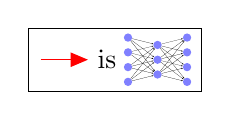
\begin{tikzpicture}
    \node at (0,0) (uses){is};
    \draw[->,red] ([xshift=-0.6cm]uses.west)  -- (uses.west);
    \node at ([xshift=0.4cm]uses.east) {\NeuralNetwork{0.15}};
    \draw[thin] (-1,-0.4) rectangle (1.2,0.4);
  \end{tikzpicture}
  }

\tikzstyle{vecArrow} = [thick, decoration={markings,mark=at position                                
   1 with {\arrow[semithick]{open triangle 60}}},                                                   
   double distance=1.4pt, shorten >= 5.5pt,                                                         
   preaction = {decorate},                                                                          
   postaction = {draw,line width=1.4pt, white,shorten >= 4.5pt}]                                    
\tikzstyle{innerWhite} = [semithick, white,line width=1.4pt, shorten >= 4.5pt]                      
         
\begin{document}





%% \section{Introduction: Expertise}

%% Human learners acquire expertise in a wide range of domains: some of
%% us become experts in calculus, or cooking, or biology, music, tennis,
%% or software engineering, to name just a few, and every child develops
%% expertise in natural language, intuitive physics~\cite{Pete?},
%% intuitive psychology (theory-of-mind), and motor control.  This
%% picture contrasts sharply with the current state of machine
%% intelligence, where a machine is built to be an expert in a single
%% domain, like boardgames~\cite{alphaGo}, medical
%% diagnosis~\cite{mycin,CNNsForDiseaseDetection}, theorem
%% proving~\cite{eurisko}, or visual object recognition~\cite{alexNet}.
%% Thus an outstanding challenge in the long-term program of building
%% more humanlike machines is to develop an algorithm that, like people,
%% autonomously acquires expertise across many different kinds of
%% domains.

%% We contribute a model of the development of expertise that combines
%% two key ingredients.  First, an expert needs a sufficiently expressive
%% knowledge representation.  Following a long tradition in cognitive
%% science and AI, we represent knowledge as programs, which prior work
%% has used to represent expertise in recognition and generation of
%% handwriting and speech~\cite{lake2015human}, intuitive theories (of
%% kinship, taxonomy, etc.)~\cite{Ullman2012}, and natural language
%% grammar and
%% semantics~\cite{DBLP:journals/cogsr/SchmidK11,piantadosi2011learning}.
%% Second, atop this program representation, experts possess two kinds of
%% domain expertise.  They have at their disposal a powerful, yet
%% specialized, repertoire of concepts and abstractions: e.g., in
%% architecture, these are concepts like `arch' or `foundation'; in
%% software engineering these are libraries of code and domain-specific
%% languages (DSLs).  Here our model represents knowledge as programs,
%% and so we identify this kind of expertise with a DSL.  Experts also
%% have knowledge of when and how to deploy these domain-specific
%% concepts efficiently when solving new problems: e.g., mathematicians
%% efficiently search the space of proofs, intuiting which lemmas are
%% appropriate when; expert chefs intuit which compositions of
%% ingredients are likely tasty, before they actually start cooking.  For
%% our model, this aspect of expertise corresponds to the ability to
%% quickly assemble new, useful programs out of its DSL.

%% We integrate these ideas into a model called DreamCoder which acquires
%% expertise through a novel kind of wake/sleep or `dream' learning. The
%% model iterates through wake cycles -- where it solves problems by
%% writing programs -- and a pair of sleep cycles: a sleep cycle that
%% grows its DSL by replaying experiences from waking and consolidating
%% them into new abstractions, and a sleep cycle that improves its
%% knowledge of how to write programs by training a neural network on
%% replayed experiences as well as `dreams', or samples, from its DSL.

%% DreamCoder builds on multiple generations of AI research, going back
%% to the 1960's~\cite{solomonoff1964formal} when program-learning was
%% proposed as a paradigm for general AI.  Broadly speaking recent work
%% has either developed neural approaches for learning to efficiently
%% deploy a fixed
%% DSL~\cite{devlin2017robustfill,balog2016deepcoder,NGDS,spiral}, or
%% developed symbolic approaches for representing and searching through
%% spaces of
%% programs~\cite{gulwani2011automating,solar2008program,DBLP:books/daglib/0070933}.
%% We were motivated by approaches that learn or grow the
%% DSL~\cite{Dechter:2013:BLV:2540128.2540316,DBLP:conf/icml/LiangJK10,solomonoff1989system,DBLP:journals/corr/abs-1110-5667,stolle2002learning}.
%% Our goal with DreamCoder is to show that the combination of
%% neurally-guided search and DSL learning is a uniquely powerful way of
%% building systems that, like human learners, autonomously acquire the
%% expertise needed to navigate a new domain of problems.





\section{Introduction}

What would it take to build a machine that can learn everything a
person does over their lifetime?
Although this goal will remain distant for the foreseeable future,
we know that a general learning system like this would need to be able to acquire many different kinds of expertise.
Virtually every child becomes an expert in natural language, motor control, and social interaction, while learning rich
intuitive theories of kinship, taxonomy and physics. Many of those
children will grow into adults with competence in cooking, calculus, tennis, drawing
pictures, or writing software.
Expertise -- the ability to quickly solve new problems in a domain -- is crucial.
Human learning goes far beyond just memorizing a large set of facts or routines,
but involves higher-order skills,
like learning to learn new concepts or
learning to solve new types of problems more quickly and effectively.
Despite great advances in machine learning,
we are still far from
an AI with these abilities.
The modern AI toolkit has given us machines that learn to play challenging games at superhuman levels,
but cannot quickly transfer to similar games like a person would;
or, which can learn to generate convincing English prose,
but which do not then learn to analyze many different languages,
like a field linguist would.
Here, we contribute a computational model that takes a small step toward the goal of building machines that
grow into domain experts,
looking at much simpler kinds of problems that humans can learn to solve and indeed become experts in.

Our model is structured
around the hypothesis that
domain expertise
consists primarily of two ingredients.
First, domain experts have 
explicit, declarative concepts that are powerful yet finely-tuned.
A visual artist has concepts like arcs, spirals, symmetries, and perspectives;
a physicist has concepts like dot products, vector fields, and conservation laws;
and an architect has concepts like arches, supports, and bridges.
Second, experts have implicit, procedural skill in deploying those concepts
to quickly solve new problems:
at a glance, human domain
experts can intuit which compositions of concepts are likely to solve
the task at hand, even before searching for a solution.
Studies of human expertise
find that,
compared to novices,
experts can quickly categorize and classify problems based on the ``deep structure''
of the problem's solution~\cite{chi1981expertise,chi2012seeing}.
In short, we take the stance that expertise means both
having the right explicit concepts, and being able to quickly see how those concepts can be composed into a solution.

Because solutions to many kinds of problems can often be described as
some kind of
program~\cite{lake2015human,Ullman2012,DBLP:journals/cogsr/SchmidK11},
our model approaches a specific problem by searching for a program solving
it. It gradually grows its explicit domain-specific knowledge for a
class of problems by assembling a library of code containing concepts
useful for the domain, and by training a neural network to quickly
infer, for a specific problem, what code in its library is likely to
solve it. We think of these two learned components as analogous to the
explicit concepts and implicit procedural skill that human experts
develop.  The model is an instance of what in the machine learning
community is called a wake-sleep algorithm, where for us, `waking'
corresponds to solving problems, while a pair of `sleep' cycles
correspond to improving the library of explicit concepts and training
the neural net to improve implicit procedural knowledge of how to
write code.


We will first investigate our model within classic program
synthesis domains for manipulating sequences of numbers and text, and
then consider visual and creative programs for drawing pictures and
building towers out of toy blocks, and finally consider programs for basic kinds of equation discovery and programming language design, altogether considering both
deterministic and probabilistic programs that act both generatively
(e.g., producing an artifact like an image or plan) and conditionally
(e.g., mapping inputs to outputs).

Our model iteratively creates new library routines that build on
concepts acquired earlier in its learning trajectory, growing a library with nested
hierarchies of code.  We think of this cumulative nesting of
abstractions as a variety of deep representation
learning~\cite{lecun2015deep}.  Figure~\ref{exampleDSL} diagrams a
subset of these learned networks (the library). For example, the model
learns to sort sequences of numbers by invoking a library component 4
layers deep, or draws the leftmost pairs of images in
Figure~\ref{exampleDSL} using a depth-3 component.  For this reason we
refer to our approach as an instance of `deep program learning'.

\begin{figure}
  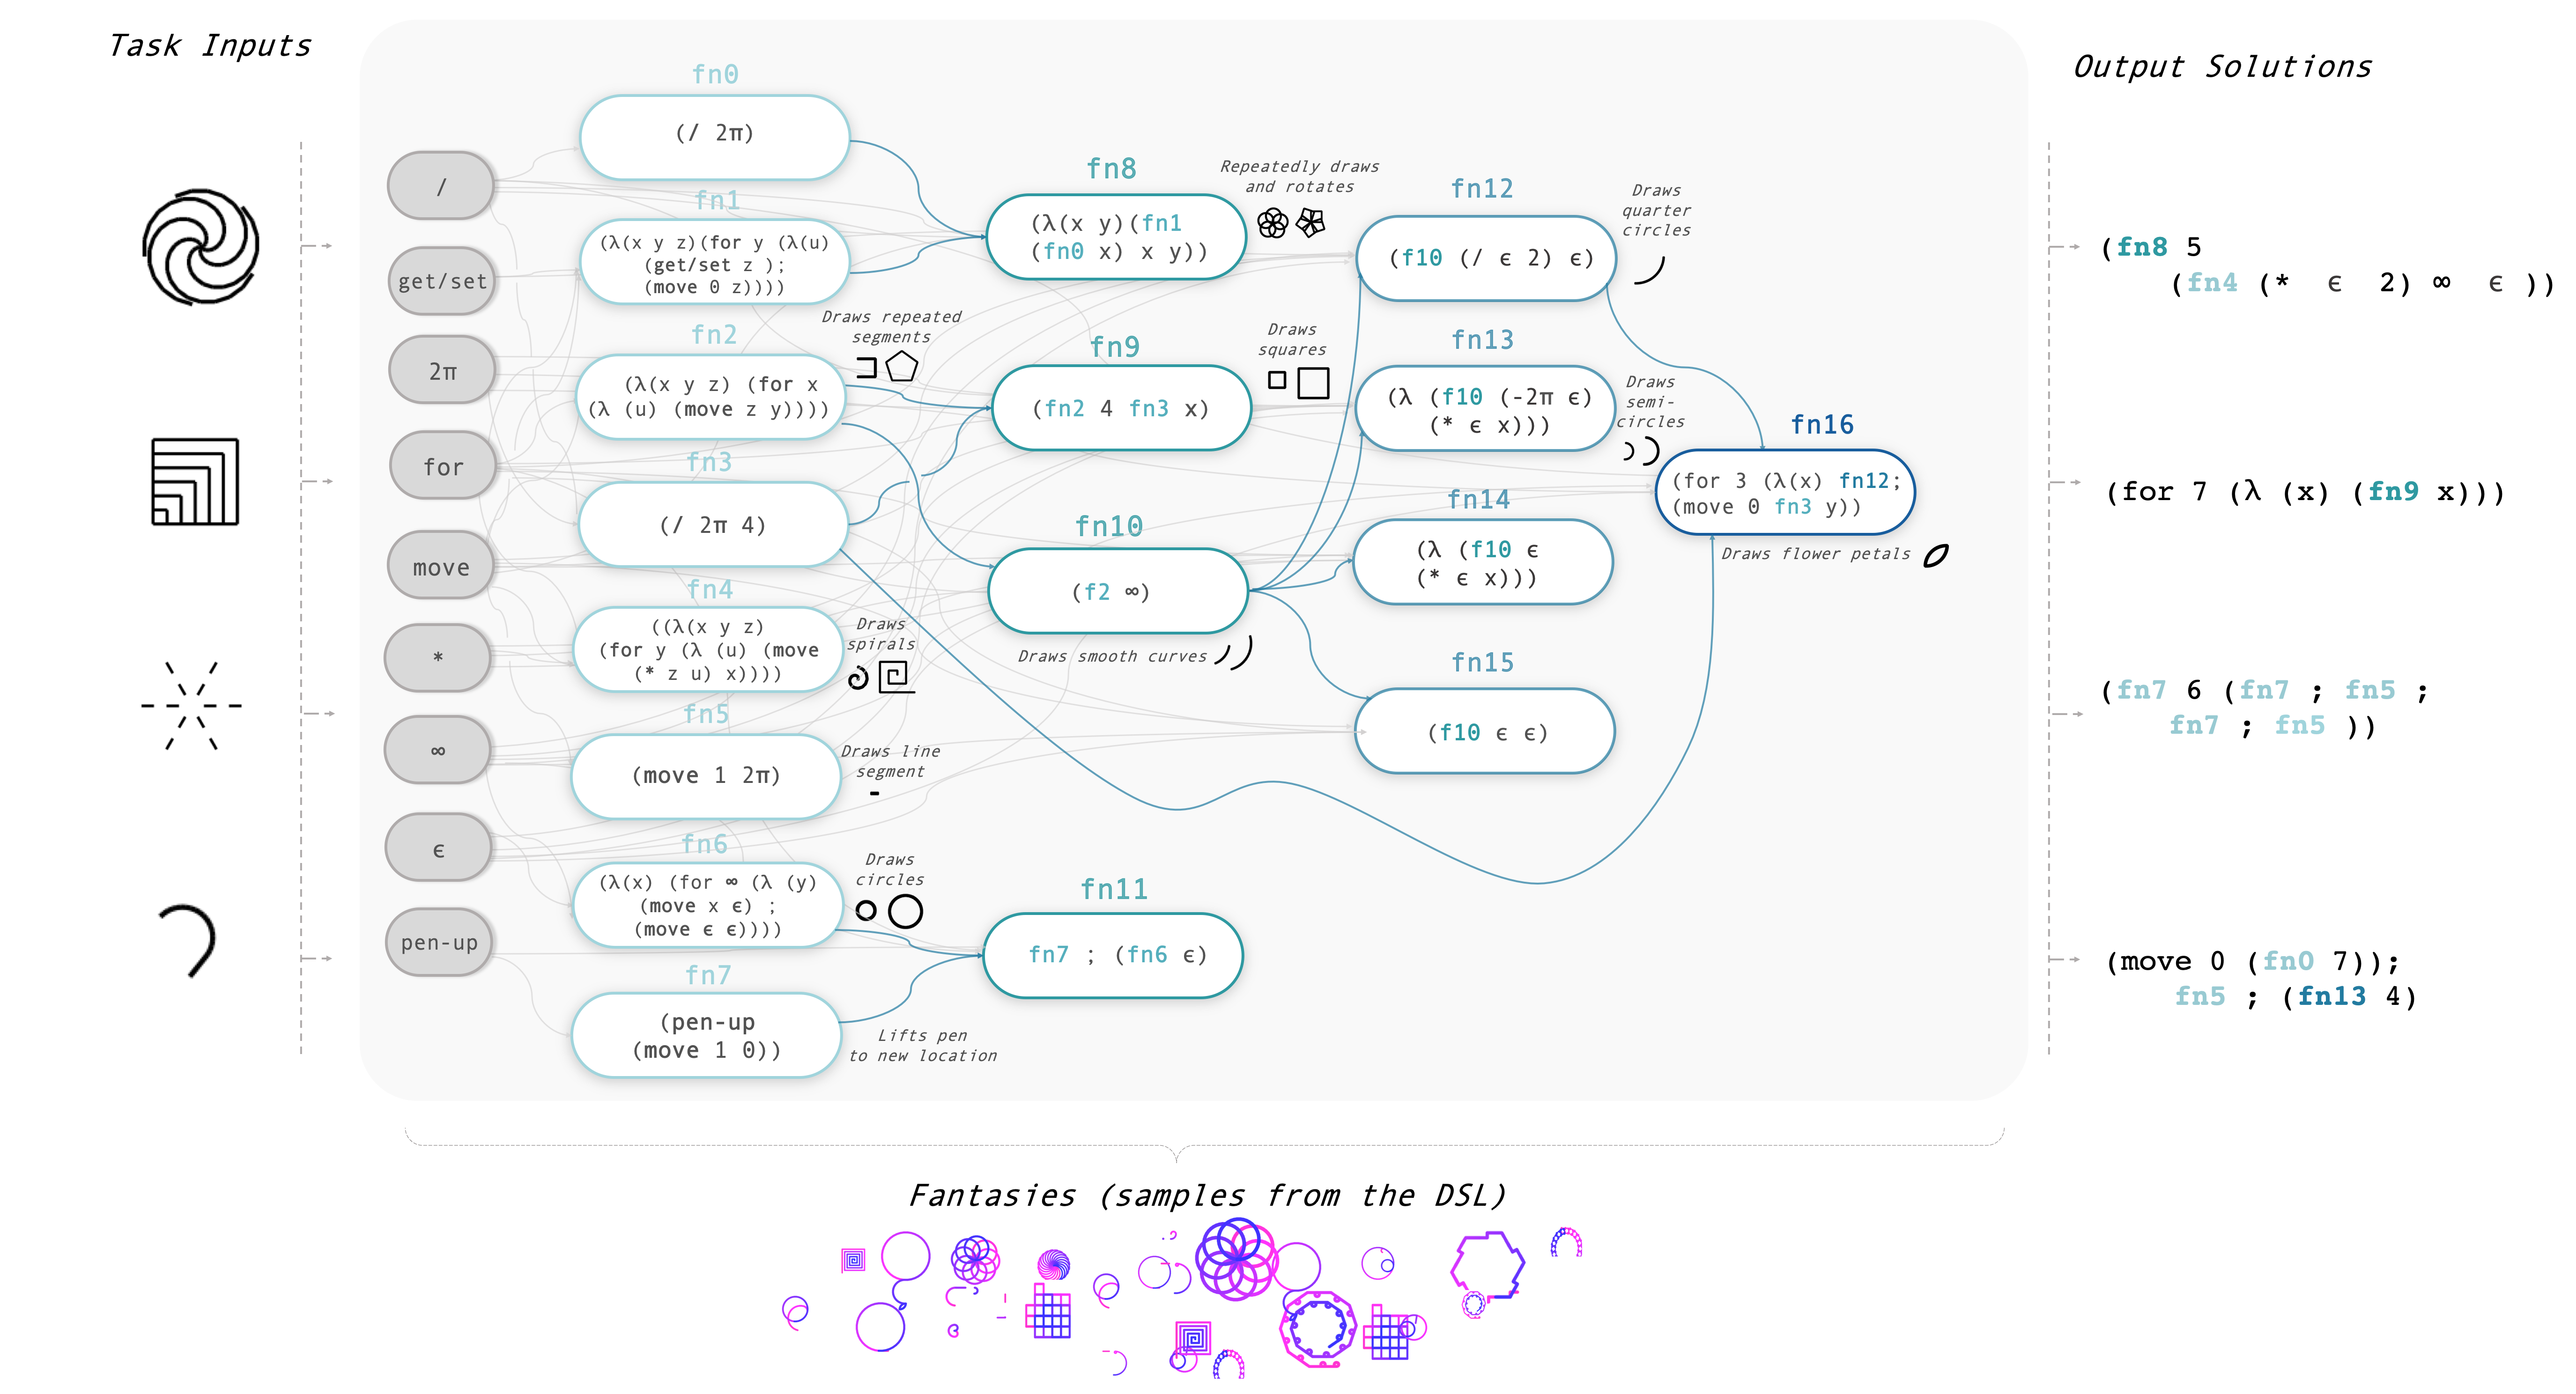
\includegraphics[width = \textwidth]{figures/DeepLogo_4_15}
  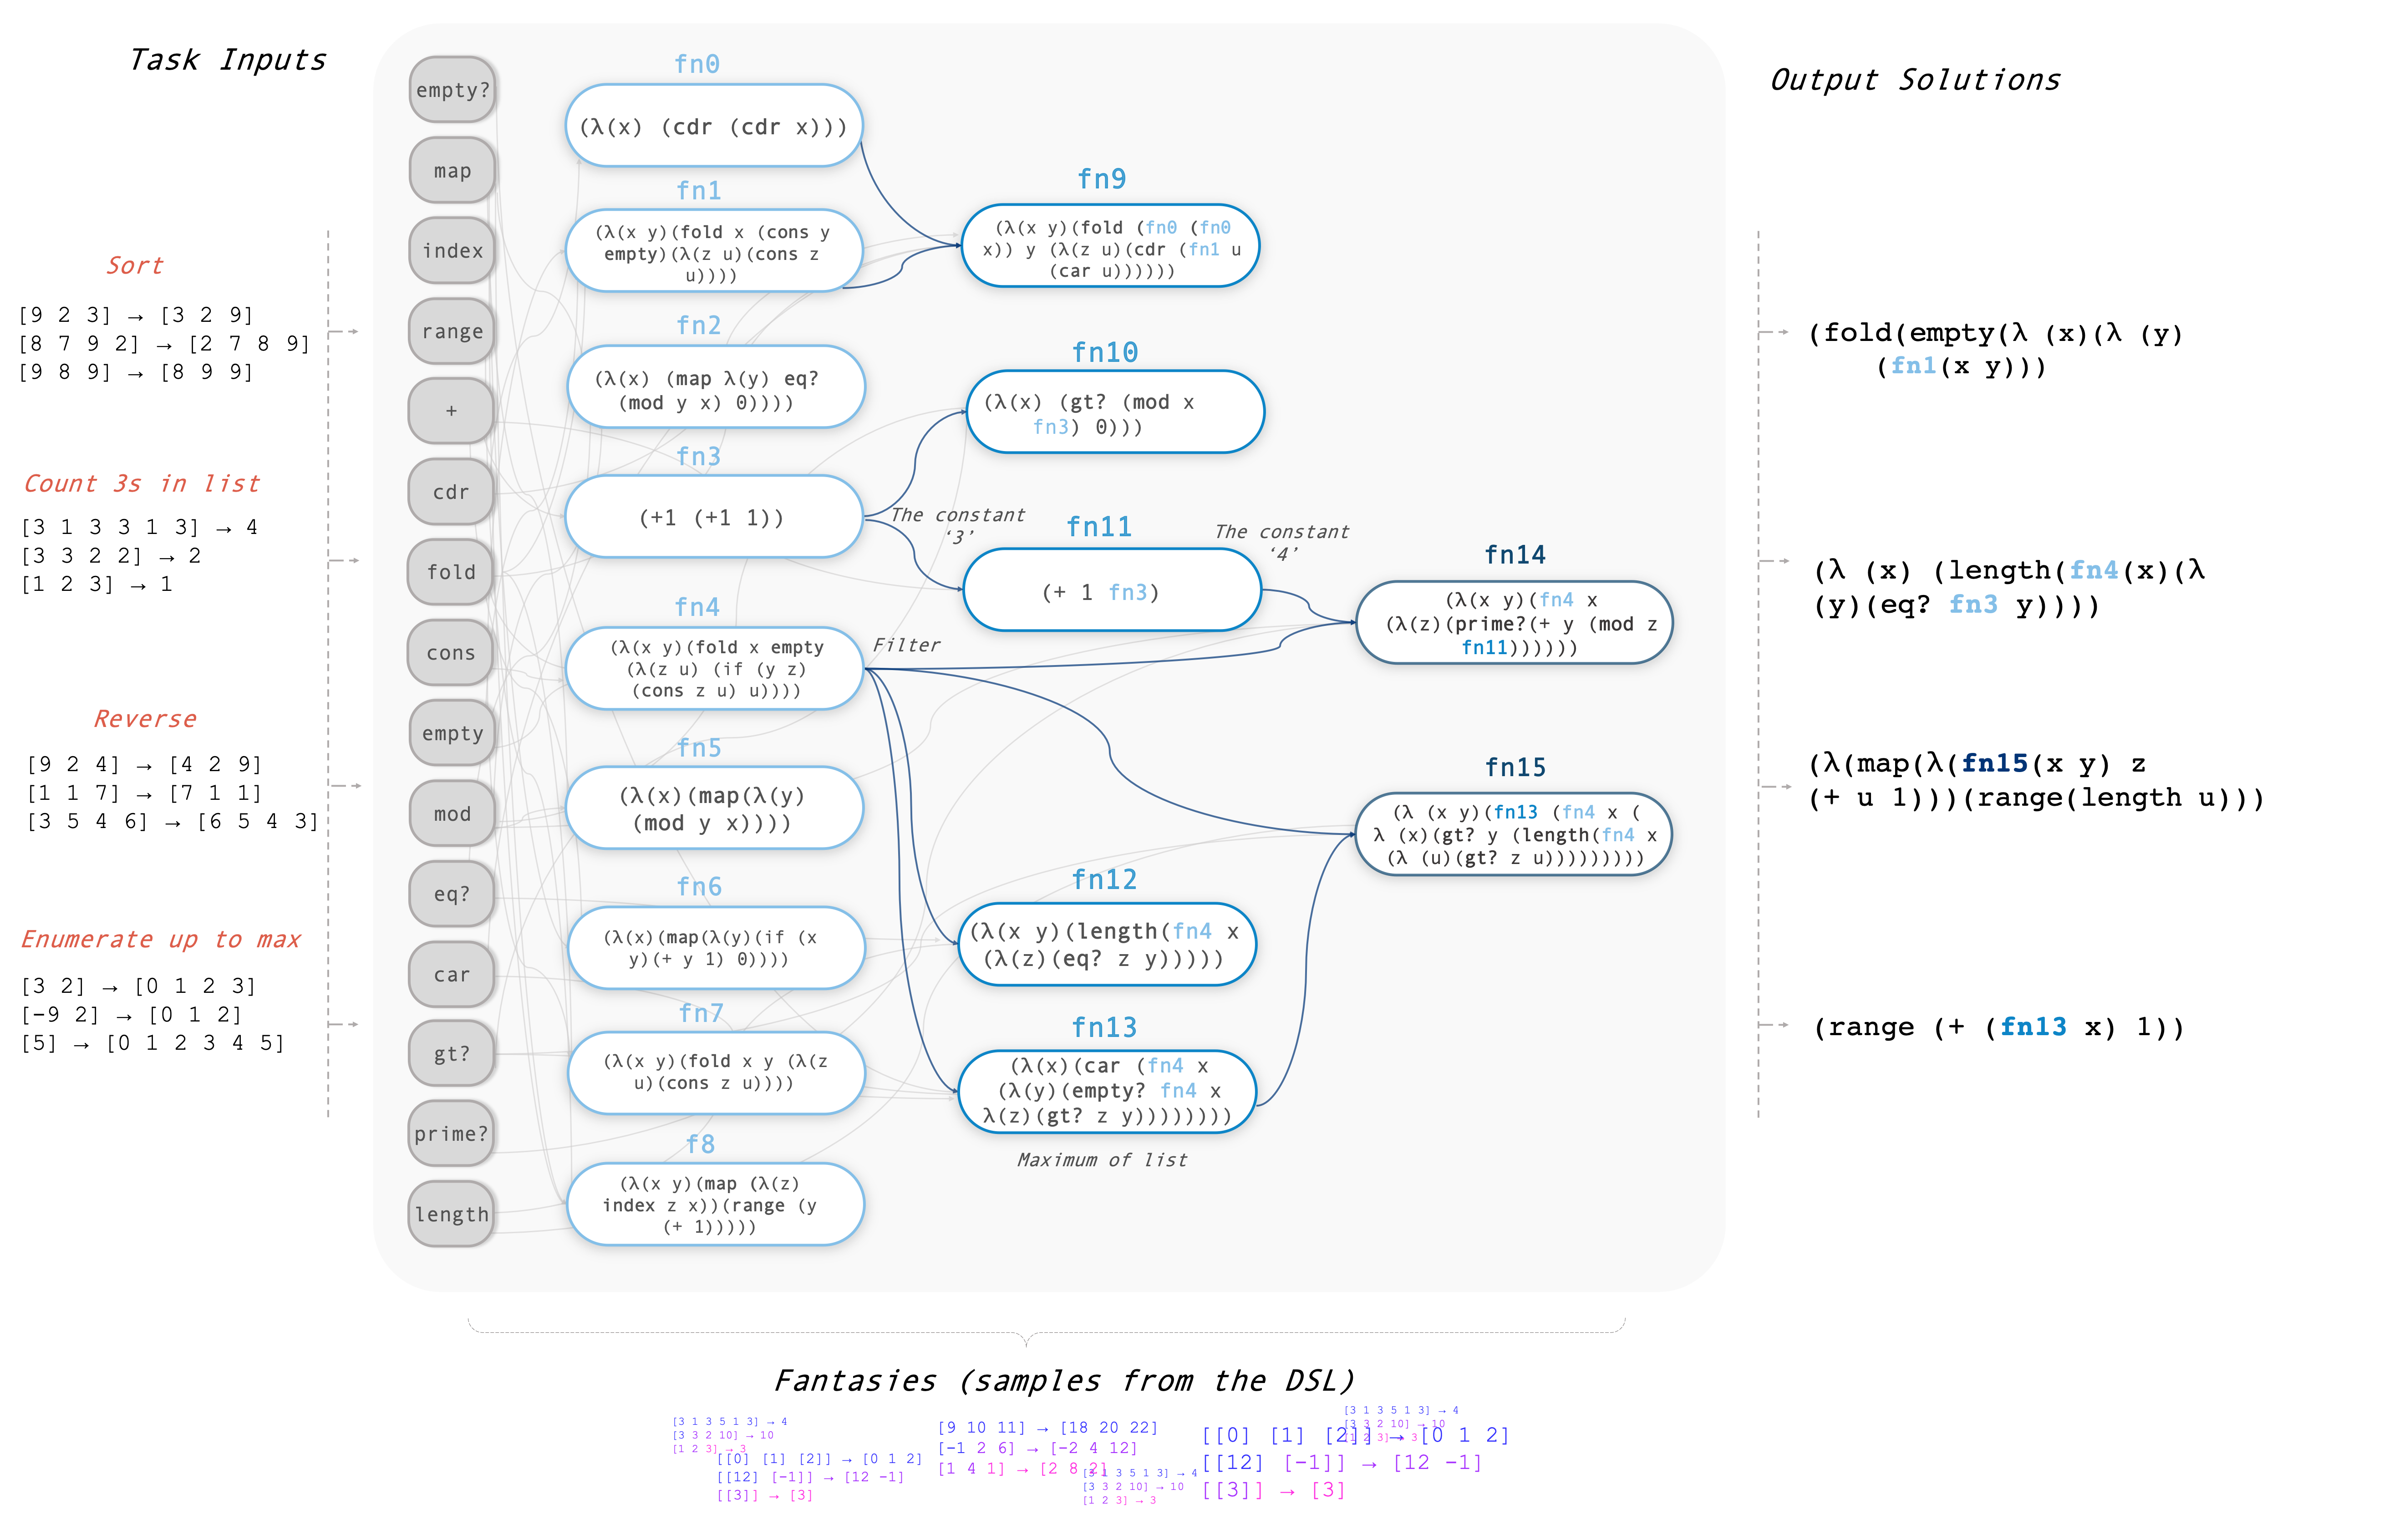
\includegraphics[width = \textwidth]{figures/DeepList_4_17}
  \caption{Model solves tasks (left; top, task is to draw an image. bottom, task is input/output mapping) by writing programs (right column) where these programs invoke explicit declarative knowledge in the form of library routines (middle) jointly learned w/ the solutions. Library code can call each other (arrows), forming a layered network of domain-specific concepts. Fantasies (below library) are tasks sampled by randomly combining code from library. Fantasies are used to train a neural net to help search for programs.}\label{exampleDSL}
\end{figure}






%% \section{Old introduction}

%% An old dream within AI is a machine that learns and reasons by writing
%% its own programs.  This vision stretches back to the
%% 1960's~\cite{solomonoff1964formal} and, if fully realized, could bring
%% us much closer to machines that learn and think like humans.
%% Computational models of cognition often explain the flexibility and
%% richness of human thinking in terms of program learning: from everyday
%% thinking and problem solving (motor program induction as an account of
%% recognition and generation of handwriting and
%% speech~\cite{lake2015human}; functional programs as a model of natural
%% language semantics~\cite{SOMETHING}) to learning problems that unfold
%% over longer developmental time scales: the child's acquisition of
%% intuitive theories (of kinship, taxonomy, etc.)~\cite{Ullman2012} and
%% natural language grammar~\cite{DBLP:journals/cogsr/SchmidK11}, to name
%% just a few.  An outstanding challenge, however, is to engineer
%% program-learners that display the same level of domain-generality as
%% the humans they are meant to model.

%% Recent program-learning systems developed within the AI and machine
%% learning community are impressive along many dimensions, authoring
%% programs for problem domains like drawing
%% pictures~\cite{spiral,ellis2017learning}, transforming
%% text~\cite{gulwani2011automating} and numerical
%% sequences~\cite{balog2016deepcoder}, robot motion
%% planning~\cite{devlin2017neural}, and reasoning over common sense
%% knowledge bases~\cite{muggleton2015meta}.  These systems work in
%% different ways, but typically hinge upon a carefully hand-engineered
%% Domain Specific Language (DSL).  The DSL restricts the space of
%% programs to contain the kinds of concepts needed for one specific
%% domain.  For example, a picture-drawing DSL could include concepts
%% like circles and spirals, and a DSL for numerical sequences could
%% include sorting and reversing lists of numbers.  Modern systems also
%% learn how to efficiently deploy the DSL on new
%% problems~\cite{devlin2017robustfill,balog2016deepcoder,NGDS}, but --
%% unlike human learners -- do not discover the underlying system of
%% concepts needed to navigate the domain.

%% We contribute a program-induction system that learns the
%% domain-specific concepts (DSL) while jointly learning how to use those
%% concepts.  This joint learning problem models two complementary
%% notions of domain expertise: domain experts have at their disposal
%% a powerful, yet specialized repertoire of concepts and abstractions
%% (analogous to the DSL) while also having accurate intuitions about
%% when and how to use those concepts to solve new problems.
%% Representative domains,
%% along with DSLs we learn for them,
%% are shown in Figure~\ref{exampleDSL}.

%% We call our system `DreamCoder' because it acquires these two kinds of
%% expertise through a novel kind of wake/sleep or `dream'
%% learning~\cite{hinton1995wake}, iterating through a wake cycle --
%% where it solves problems by writing programs -- and a pair of sleep
%% cycles, both of which are loosely biologically inspired by actual
%% sleep.  The first sleep cycle, which we refer to as
%% \textbf{consolidation}, grows the DSL by replying experiences from
%% waking and consolidating them into new code abstractions.  This cycle
%% is inspired by the formation of abstractions during sleep memory
%% consolidation~\cite{DUDAI201520}.  The second sleep cycle, which we
%% refer to as \textbf{dreaming}, improves the agents knowledge of how to
%% write code by training a neural network to help search for
%% programs. The neural net is trained on replayed experiences as well as
%% `fantasies', or samples, from the DSL.  These two kinds of dreams are
%% inspired by the distinct episodic replay and hallucination components
%% of dream sleep~\cite{fosse2003dreaming}.


%% This dream-learning architecture brings together two lines of prior work,
%% both of which have been separately influential within
%% artificial intelligence.
%% One line of work
%% considers the problem of learning new concepts, abstractions, or
%% `options' from
%% experience~\cite{Dechter:2013:BLV:2540128.2540316,DBLP:conf/icml/LiangJK10,solomonoff1989system,DBLP:journals/corr/abs-1110-5667,stolle2002learning},
%% while the other line of work considers the problem of learning how to
%% deploy those concepts
%% efficiently~\cite{devlin2017robustfill,balog2016deepcoder,NGDS}.  Our
%% goal with DreamCoder is to show that the combination of these ideas is
%% uniquely powerful, and pushes us toward program-writing systems that,
%% like human learners, autonomously acquire the expertise needed to
%% navigate a new domain of problems.


%% Each wake/sleep cycle creates new DSL components that build on
%% components learned in earlier sleep cycles, growing a DSL with nested 
%% hierarchies of code.  We identify this cumulative nesting of
%% abstractions as a variety of deep representation
%% learning~\cite{lecun2015deep}.  Figure~\ref{exampleDSL} diagrams a
%% subset of these learned networks (the DSL). For example, the system
%% learns to sort sequences of numbers by invoking a DSL component 4
%% layers deep, or draws the leftmost pairs of images in
%% Figure~\ref{exampleDSL} using a depth-3 component.  For this reason we
%% refer to \system as an instance of `deep program learning'.


%% Our goal with \system is to engineer a system that develops domain
%% expertise in humanlike ways. This involves learning both declarative and
%% procedural knowledge, like a DSL and a recognition model, but includes
%% other features of the development of expertise:
%% humans can become experts in many fields,
%% and so we evaluate our algorithm across six different problem domains;
%% a human expert doesn't become an expert overnight,
%% and needs more than a handful of example problems to learn from,
%% but doesn't need millions of examples;
%% similarly our algorithm's
%% learning trajectory unfolds over a series of wake/sleep cycles
%% requiring around a hundred problems per domain.


%\begin{figure}
  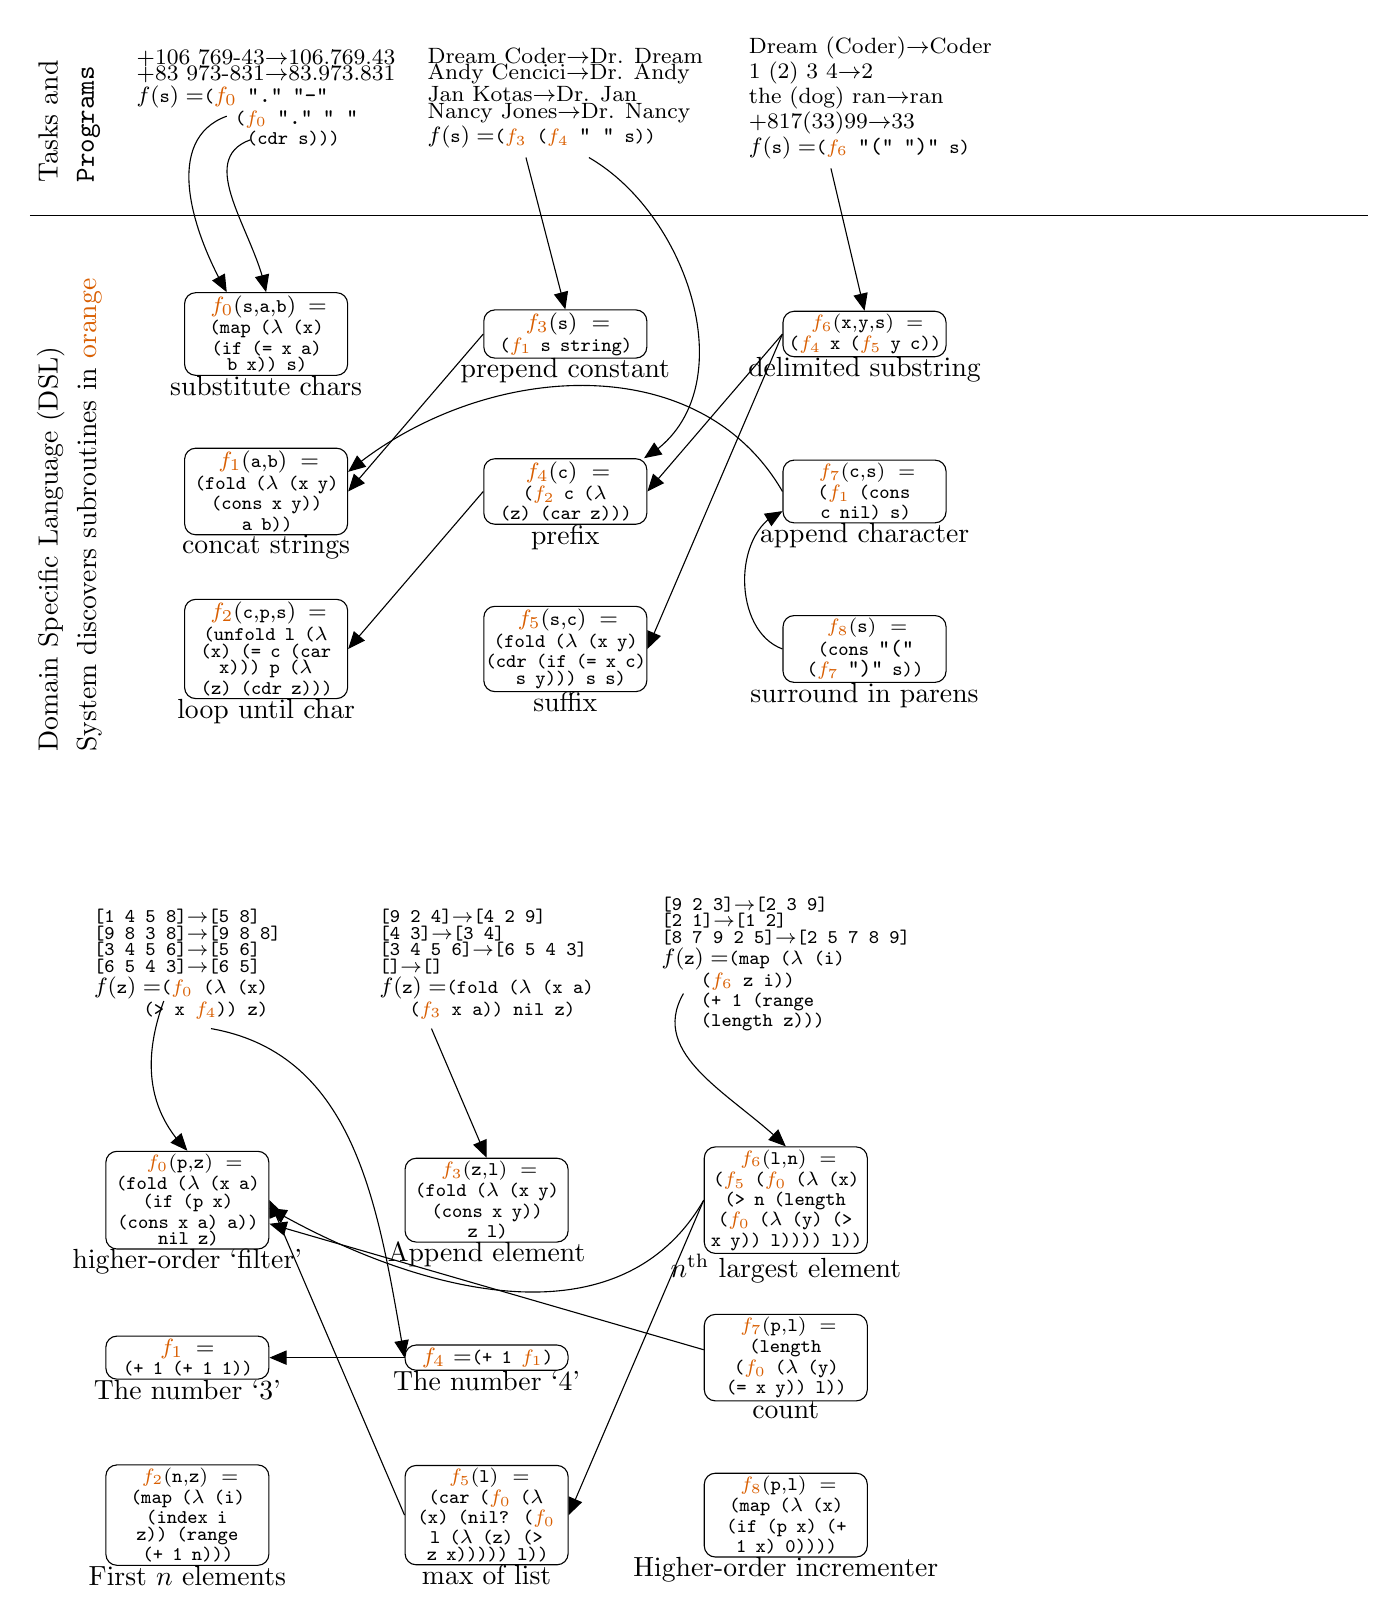
\begin{tikzpicture}
    \renewcommand{\baselinestretch}{0.5}
    \newcommand{\inventionColor}{orange}
    \newcommand{\name}[2]{
      \mcode{{\color{\inventionColor}$f_{#1}$}$($#2$)\,=\,$}
    }
    \newcommand{\noArguments}[1]{
      \mcode{{\color{\inventionColor}$f_{#1}\,=\,$}}
    }

    
    \newcommand{\horizontalSpacing}{3.8cm}
    \newcommand{\verticalSpacing}{2cm}

    
%    \draw (0,0) rectangle (10,5);
    \node(t1)[align=left] at (1,-1) {
      \footnotesize +106 769-43$\to $106.769.43\\
      \footnotesize +83 973-831$\to $83.973.831\\
      \footnotesize $f(\text{\mcode{s}}) = $\mcode{(}\subnode{f01}{${\color{\inventionColor}f_0}$}\mcode{  \codechar{.} \codechar{-}}\\
      \footnotesize \hspace{1.25cm}\mcode{(${\color{\inventionColor}f_0}$ \codechar{.} \codechar{ }}\\
      \footnotesize \hspace{1.4cm}\mcode{(cdr s)))}
    };
    \node(t2)[align=left,anchor=center] at ([xshift=\horizontalSpacing]t1.center) {
      \footnotesize Dream Coder$\to$Dr. Dream\\
      \footnotesize Andy Cencici$\to$Dr. Andy\\
      \footnotesize Jan Kotas$\to$Dr. Jan\\
      \footnotesize Nancy Jones$\to$Dr. Nancy\\
      \footnotesize $f(\text{\mcode{s}}) = $\mcode{(${\color{\inventionColor}f_3}$ (${\color{\inventionColor}f_4}$ \codechar{ } s))}
    };
    \node(t3)[align=left] at ([xshift=2cm]t2.east) {
      \footnotesize Dream (Coder)$\to$Coder\\
      \footnotesize 1 (2) 3 4$\to$2\\
      \footnotesize the (dog) ran$\to$ran\\
      \footnotesize +817(33)99$\to$33\\
      \footnotesize $f(\text{\mcode{s}}) = $\mcode{(${\color{\inventionColor}f_6}$ \codechar{(} \codechar{)} s)}
    };

    \draw (-2,-2.5) -- (15,-2.5);
    \node[align=left,rotate=90] at (-1.5,-1.3) {Tasks and\\\\\texttt{Programs}};

    \node[align=left,rotate=90] at (-1.5,-6.3) {Domain Specific Language (DSL)\\\\System discovers subroutines in {\color{\inventionColor}orange}};

    
    \newcommand{\invention}[4]{
      \node(#1)[inner sep=1,anchor=center,text width=2cm,draw,rounded corners,align=center] at (#2) {
        \footnotesize #3
      };
      \node[anchor=north] at ([yshift=3.5pt]#1.south) {#4};
    }
    \newcommand{\vinvention}[4]{
      \invention{#1}{[yshift=-\verticalSpacing]#2.center}{#3}{#4}
    }
    \newcommand{\hinvention}[4]{
      \invention{#1}{[xshift=\horizontalSpacing]#2.center}{#3}{#4}
    }


    \invention{substitution}{1,-4}{
      ${\color{\inventionColor}f_0}($\mcode{s}$,$\mcode{a}$,$\mcode{b}$) \,=\, $\\
       \mcode{(map ($\lambda$ (x) (if (= x a)\\ b x)) s)}
    }{substitute chars}
    \vinvention{cat}{substitution}{
      ${\color{\inventionColor}f_1}($\mcode{a}$,$\mcode{b}$) \,=\, $\\
      \mcode{(fold ($\lambda$ (x y)\\ (cons x y))\\ a b))}
    }{concat strings}
    \vinvention{looping}{cat}{
       ${\color{\inventionColor}f_2}($\mcode{c}$,$\mcode{p}$,$\mcode{s}$) \,=\, $\\
      \mcode{(unfold l ($\lambda$ (x) (= c (car x))) p ($\lambda$ (z) (cdr z)))}
    }{loop until char}

    \hinvention{constant}{substitution}{
      ${\color{\inventionColor}f_3}($\mcode{s}$) \,=\, $\\
      \mcode{(${\color{\inventionColor}f_1}$ s string)}
    }{prepend constant}
    \vinvention{drop}{constant}{
      ${\color{\inventionColor}f_4}($\mcode{c}$) \,=\, $\\
      \mcode{(${\color{\inventionColor}f_2}$ c ($\lambda$ }\\\mcode{(z) (car z)))}
    }{prefix}
    \vinvention{suffix}{drop}{
      ${\color{\inventionColor}f_5}($\mcode{s}$,$\mcode{c}$) \,=\, $\\
      \mcode{(fold ($\lambda$ (x y) }\\\mcode{(cdr (if (= x c)}\\\mcode{ s y))) s s)}
    }{suffix}

    \hinvention{delimited}{constant}{
      \mcode{${\color{\inventionColor}f_6}($x$,$y$,$s$)\,=\,$}\\
      \mcode{(${\color{\inventionColor}f_4}$ x (${\color{\inventionColor}f_5}$ y c))}
    }{delimited substring}
    \draw[->] (delimited.west) -- (drop.east);
    \draw[->] (delimited.west) -- (suffix.east);

    \vinvention{appendSingle}{delimited}{
      \mcode{${\color{\inventionColor}f_7}($c$,$s$)\,=\,$}\\
      \mcode{(${\color{\inventionColor}f_1}$ (cons c nil) s)}}{append character}
    
    \vinvention{surround}{appendSingle}{
      \mcode{${\color{\inventionColor}f_8}($s$)\,=\,$}\\
      \mcode{(cons \codechar{(} (${\color{\inventionColor}f_7}$ \codechar{)} s))}}{surround in parens}
    \draw[->] (surround.west) to[in=200,out=160] ([yshift=-0.25cm]appendSingle.west);
    \draw[->] (appendSingle.west) to[in=40,out=120] ([yshift=0.25cm]cat.east);
    
    \draw[->] (drop.west) -- (looping.east);
    \draw[->] (constant.west) -- (cat.east);

    \draw[->] ([xshift=-0.5cm]t2.south) -- (constant.north);
    \draw[->] ([xshift=0.3cm]t2.south) to[in=30,out=-30] ([xshift=1cm]drop.north);

    \draw[->] ([yshift=0.2cm,xshift=-0.2cm]t1.south) to[in=100,out=200] (substitution.north);
    \draw[->] ([yshift=0.5cm,xshift=-0.5cm]t1.south) to[in=120,out=200] ([xshift=-0.5cm]substitution.north);
    \draw[->] ([xshift=-0.5cm]t3.south) -- (delimited.north);
          
    \begin{scope}[shift={(0,-15)}]
      \invention{filter}{0,0}{
        \name{0}{p$,$z}\mcode{\\(fold ($\lambda$ (x a)\\ (if (p x) (cons x a) a))\\ nil z)} 
        }{higher-order `filter'}

      \vinvention{three}{filter}{\footnotesize ${\color{\inventionColor}f_1} = $\\\mcode{(+ 1 (+ 1 1))}}{The number `3'}
      \vinvention{prefix}{three}{\name{2}{n$,$z}\\\mcode{(map ($\lambda$ (i) (index i z)) (range (+ 1 n)))}}{First $n$ elements}
      \hinvention{single}{filter}{\name{3}{z$,$l}\\\mcode{(fold ($\lambda$ (x y)\\(cons x y))\\ z l)}}{Append element}
      \vinvention{for}{single}{\footnotesize ${\color{\inventionColor}f_4} = $\mcode{(+ 1 ${\color{\inventionColor}f_1}$)}}{The number `4'}
      \vinvention{Max}{for}{\name{5}{l}\\\mcode{%
          (car (${\color{\inventionColor}f_0}$ ($\lambda$ (x) (nil? (${\color{\inventionColor}f_0}$ l ($\lambda$ (z) (> z x))))) l))}}{max of list}
      \hinvention{largest}{single}{\name{6}{l$,$n}\\\mcode{(${\color{\inventionColor}f_5}$ (${\color{\inventionColor}f_0}$ ($\lambda$ (x) \\(> n (length (${\color{\inventionColor}f_0}$ ($\lambda$ (y) (> x y)) l)))) l))}}{$n^{\text{th}}$ largest element}
      \vinvention{count}{largest}{\name{7}{p$,$l}\\\mcode{(length\\ (${\color{\inventionColor}f_0}$ ($\lambda$ (y) (= x y)) l))}}{count}
      \vinvention{weird}{count}{\name{8}{p$,$l}\mcode{
          (map ($\lambda$ (x) (if (p x) (+ 1 x) 0))))}}
                 {Higher-order incrementer}

      \draw[->] (for.west) -- (three.east);
      \draw[->] ([yshift=-0.0cm]largest.west) -- (Max.east);
      \draw[->] ([yshift=-0.cm]largest.west) to[out=240,in=330] ([yshift=-0.1cm]filter.east);
      \draw[->] (Max.west) -- (filter.east);
      \draw[->] ([yshift=0.1cm]count.west) -- ([yshift=-0.3cm]filter.east);

      \node(t1)[align=left,anchor=center] at (0,3) {
        \mcode{[1 4 5 8]$\to$[5 8]}\\
        \mcode{[9 8 3 8]$\to$[9 8 8]}\\
        \mcode{[3 4 5 6]$\to$[5 6]}\\
        \mcode{[6 5 4 3]$\to$[6 5]}\\
        \footnotesize $f(\text{\mcode{z}}) = $\mcode{(${\color{\inventionColor}f_0}$ ($\lambda$ (x)}\\\hspace{0.5cm}\mcode{ (> x ${\color{\inventionColor}f_4}$)) z)}
      };
      \node(t2)[align=left] at ([xshift=\horizontalSpacing]t1.center) {
        \mcode{[9 2 4]$\to$[4 2 9]}\\
        \mcode{[4 3]$\to$[3 4]}\\
        \mcode{[3 4 5 6]$\to$[6 5 4 3]}\\
        \mcode{[]$\to$[]}\\
        \footnotesize $f(\text{\mcode{z}}) = $\mcode{(fold ($\lambda$ (x a)}\\\hspace{0.25cm}\mcode{ (${\color{\inventionColor}f_3}$ x a)) nil z)}
      };
      \node(t3)[align=left] at ([xshift=\horizontalSpacing]t2.center) {
        \mcode{[9 2 3]$\to$[2 3 9]}\\
        \mcode{[2 1]$\to$[1 2]}\\
        \mcode{[8 7 9 2 5]$\to$[2 5 7 8 9]}\\
        \footnotesize $f(\text{\mcode{z}}) = $\mcode{(map ($\lambda$ (i)}\\\hspace{0.5cm}\mcode{(${\color{\inventionColor}f_6}$ z i)) }\\\hspace{0.5cm}\mcode{(+ 1 (range }\\\hspace{0.5cm}\mcode{(length z)))}
      };

      \draw[->] ([yshift=0.35cm,xshift=-0.3cm]t1.south) to[out=250] (filter.north);
      \draw[->] ([yshift=0.0cm,xshift=0.3cm]t1.south) to[out=350,in=100] (for.west);
      \draw[->] ([xshift=-0.7cm]t2.south) -- (single.north);
      \draw[->] ([xshift=-1.3cm,yshift=0.6cm]t3.south) to[out=240] (largest.north);

    \end{scope}
    
    

    

    \end{tikzpicture}
\end{figure}

\begin{figure}\centering
  \begin{tikzpicture}
    \renewcommand{\baselinestretch}{0.5}
    \newcommand{\inventionColor}{orange}

    \newcommand{\name}[2]{
      \mcode{{\color{\inventionColor}$f_{#1}$}$($#2$)\,=\,$}
    }
    \newcommand{\noArguments}[1]{
      \mcode{{\color{\inventionColor}$f_{#1}$}$\,=\,$}
    }
    \newcommand{\use}[1]{{\color{\inventionColor}$f_{#1}$}}
    \newcommand{\horizontalSpacing}{4.2cm}
    \newcommand{\verticalSpacing}{2cm}
    
    \newcommand{\invention}[4]{
      \node(#1)[inner sep=1,anchor=south,text width=2.2cm,ellipse,draw,rounded corners,align=center] at (#2) {
        \footnotesize #3
      };
      \node[anchor=north,align=center] at ([yshift=3.5pt]#1.south) {#4};
    }
    \newcommand{\vinvention}[4]{
      \invention{#1}{[yshift=-\verticalSpacing]#2.south}{#3}{#4}
    }
    \newcommand{\hinvention}[4]{
      \invention{#1}{[xshift=\horizontalSpacing]#2.south}{#3}{#4}
    }
    \newcommand{\exampleFunction}[2]{
      \includegraphics[width = 0.5cm]{#1}, \includegraphics[width = 0.5cm]{#2}
    }
    \newcommand{\task}[4]{
      \node[align=left,anchor=center](t#1) at (#2) {#3};
      \node[align=left](p#1) at ([yshift=-0.75cm]t#1.south) {#4};
    }
    \newcommand{\nextTask}[4]{
      \task{#1}{[xshift=\horizontalSpacing]#2.center}{#3}{#4}
    }

    \begin{scope}[shift={(0,8)}]
      \task{1}{2,3}{
        \textsc{Reverse}\\
        \mcode{[9 2 4]$\to$[4 2 9]}\\
        \mcode{[4 3]$\to$[3 4]}\\
        \mcode{[3 4 5 6]$\to$[6 5 4 3]}\\
        \mcode{[]$\to$[]}
      }{\footnotesize $f(\text{\mcode{z}}) = $\mcode{(fold ($\lambda$ (x a)}\\\hspace{0.25cm}\mcode{ (${\color{\inventionColor}f_3}$ x a)) nil z)}}
      \nextTask{2}{t1}{
        \textsc{Take if $\geq 5$}\\
        \mcode{[1 4 5 8]$\to$[5 8]}\\
        \mcode{[9 8 3 8]$\to$[9 8 8]}\\
        \mcode{[3 4 5 6]$\to$[5 6]}\\
        \mcode{[6 5 4 3]$\to$[6 5]}
      }{\footnotesize $f(\text{\mcode{z}}) = $\mcode{(${\color{\inventionColor}f_0}$ ($\lambda$ (x)}\\\hspace{0.5cm}\mcode{ (> x ${\color{\inventionColor}f_4}$)) z)}}
      
      \nextTask{3}{t2}{
        \textsc{Sort}\\
        \mcode{[9 2 3]$\to$[2 3 9]}\\
        \mcode{[2 1]$\to$[1 2]}\\
        \mcode{[8 7 9 2 5]$\to$[2 5 7 8 9]}\\
        \mcode{[9 8 9]$\to$[8 9 9]}
      }{\footnotesize $f(\text{\mcode{z}}) = $\mcode{(map ($\lambda$ (i)}\\\hspace{0.5cm}\mcode{(${\color{\inventionColor}f_6}$ z i)) }\\\hspace{0.5cm}\mcode{(+ 1 (range }\\\hspace{0.5cm}\mcode{(length z)))}}

      %% \vinvention{filter}{p1}{
      %%   \name{0}{p$,$z}\mcode{\\(fold ($\lambda$ (x a)\\ (if (p x) (cons x a) a))\\ nil z)} 
      %% }{higher-order `filter'}
      \vinvention{single}{p1}{\name{3}{z$,$l}\\\mcode{(fold ($\lambda$ (x y)\\(cons x y))\\ z l)}}{Append element}

      \vinvention{three}{single}{\footnotesize \noArguments{1}\\\mcode{(+ 1 (+ 1 1))}}{The number `3'}
      \vinvention{prefix}{three}{\name{2}{n$,$z}\\\mcode{(map ($\lambda$ (i) (index i z)) (range (+ 1 n)))}}{First $n$ elements}
      \hinvention{filter}{single}{
        \name{0}{p$,$z}\mcode{\\(fold ($\lambda$ (x a)\\ (if (p x) (cons x a) a))\\ nil z)} 
      }{higher-order `filter'}
      \vinvention{for}{filter}{\noArguments{4}\\\mcode{(+ 1 ${\color{\inventionColor}f_1}$)}}{The number `4'}
      \vinvention{weird}{for}{\name{8}{p$,$l}\mcode{
          (map ($\lambda$ (x) (if (p x) (+ 1 x) 0)))}}{Higher-order incrementer}                 
      \hinvention{largest}{filter}{\name{6}{l$,$n}\\\mcode{(${\color{\inventionColor}f_5}$ (${\color{\inventionColor}f_0}$ ($\lambda$ (x) \\(> n (length (${\color{\inventionColor}f_0}$ ($\lambda$ (y) (> x y)) l)))) l))}}{$n^{\text{th}}$ largest element}
      \vinvention{Max}{largest}{\name{5}{l}\\\mcode{%
          (car (${\color{\inventionColor}f_0}$ ($\lambda$ (x) (nil? (${\color{\inventionColor}f_0}$ l ($\lambda$ (z) (> z x))))) l))}}{max of list}
      \vinvention{count}{Max}{\name{7}{p$,$l}\\\mcode{(length\\ (${\color{\inventionColor}f_0}$ ($\lambda$ (y) (= x y)) l))}}{count}

      \node[rotate=90,align=center] at ([xshift=-2cm]t1.center) {\textbf{\textsc{Tasks}}\\};
      \node(programLabel)[rotate=90,align=center] at ([xshift=-2cm]p1.center) {\texttt{\textbf{Progs.}}\\};
      \node[rotate=90,align=center] at ([xshift=-2cm]three.center) {\textbf{\textsc{Domain Specific Language}}\\
        \small Learned routines in {\color{orange}orange}};
      \node at ([yshift=0.5cm]t2.north) {\textbf{\Large \textsc{Domain: List Processing}}};

      \draw [dashed] ([xshift=0.5cm,yshift=-0.25\verticalSpacing]programLabel.east) -- ([xshift=15cm,yshift=-0.25\verticalSpacing]programLabel.east);
    \node[align=left,anchor=center] at ([xshift=14cm,yshift=-0.3\verticalSpacing]programLabel.east) {\large $\uparrow$\;system inputs\\\\\\\large $\downarrow$\;system outputs};


      \draw[->] (for.west) -- (three.east);
      \draw[->] (largest.east) to[out=0,in=0] (Max.east);
      \draw[->] ([yshift=-0.cm]largest.west) -- ([yshift=0.2cm]filter.east);
      \draw[->] (Max.west) -- (filter.east);
      \draw[->] ([yshift=0.1cm]count.west) -- ([yshift=-0.3cm]filter.east);


      \draw[->] ([yshift=0.35cm,xshift=-0.3cm]p2.south) to[out=250] (filter.north);
      \draw[->] ([yshift=0.0cm,xshift=0.3cm]p2.south) to[out=350,in=0] (for.east);
      \draw[->] ([xshift=-0.7cm]p1.south) -- (single.north);
      \draw[->] ([xshift=-1.3cm,yshift=0.6cm]p3.south) to[out=240] (largest.north);

      
    \end{scope}
    
    \renewcommand{\task}[4]{
      \node(t#1) at (#2) {\includegraphics[width = 2cm]{#3}};
      \node(p#1) at ([yshift=-0.75cm]t#1.south) {#4};
    }
    \newcommand{\nextTask}[4]{
      \task{#1}{[xshift=\horizontalSpacing]#2.center}{#3}{#4}
    }
    
    
    \task{1}{2,0}{figures/logoTasks/logo144.png}{\mcode{(for (i 4) (\use{3} i))}}
    \nextTask{2}{t1}{figures/logoTasks/logo121.png}{\mcode{(\use{7} 6 (\use{1}; (\use{0} 1)))}}
    \nextTask{3}{t2}{figures/logoTasks/logo133.png}{\mcode{(\use{7} 7 (\use{8}; \use{6}))}}
    
    \vinvention{circle}{p1}{
      \name{0}{r}\mcode{(for (i $\infty$) (move r $\epsilon$) (move $\epsilon$ $\epsilon$))}
    }{circle\\\exampleFunction{figures/logoTasks/logo51}{figures/logoTasks/logo63_dilated}}
    \vinvention{pu}{circle}{
      \noArguments{1}\mcode{(pen-up (move 1 0))}
    }{pick up pen\\and move}
    \vinvention{repeated}{pu}{
      \name{2}{n$,$d$,$a}\mcode{(for (i n) (move d a))}
    }{repeated segment\\\exampleFunction{figures/logoTasks/logoDemo1_dilated}{figures/logoTasks/logoDemo0_dilated.png}}
    \hinvention{square}{circle}{
      \name{3}{d}\mcode{(\use{2} 4 d (/ $2\pi$ 4))}
    }{square\\\exampleFunction{figures/logoTasks/logo139_dilated}{figures/logoTasks/logo142_dilated}}
    \vinvention{smooth}{square}{
      \name{4}{d$,$a}\mcode{(\use{2} $\infty$ d a)}
    }{Smooth curve\\\exampleFunction{figures/logoTasks/logoDemo2_dilated}{figures/logoTasks/logoDemo3_dilated}}
    \vinvention{angle}{smooth}{
      \name{5}{n}\mcode{(/ $2\pi$ n)}
    }{$\frac{2\pi}{n}$}
    \hinvention{semi}{square}{
      \noArguments{6}\mcode{(\use{4} $\epsilon$ $\epsilon$)}
    }{semicircle\\\exampleFunction{figures/logoTasks/logo55_dilated}{figures/logoTasks/logo62_dilated}}
    \vinvention{snow}{semi}{
      \name{7}{n$,$f}\mcode{(for (i n) \\(move 0 (\use{5} n))\\ (get/set f))}
    }{rotational symmetry\\\exampleFunction{figures/logoTasks/logo119_dilated}{figures/logoTasks/logo68_dilated}}
    \vinvention{line}{snow}{
      \noArguments{8}\mcode{(move 1 0)}
    }{line segment}

    \draw[->] (p1.south) -- (square.north);
    \draw[->] (p2.south) -- (circle.north);
    \draw[->] (p3.south) -- (semi.north);
    \draw[->] (p2.south) -- (snow.west);
    \draw[->] (p2.south) -- (pu.east);
    \draw[->] (p3.south) to[out=190,in=120] (line.west);
    \draw[->] (p3.south) to[out=200,in=120] (snow.west);

    \draw[->,orange] (snow.west) -- (angle.east);
    \draw[->,orange] (smooth.west) -- (repeated.east);
    \draw[->,orange] (semi.west) -- (smooth.east);
    \draw[->,orange] (square.west) -- (repeated.east);

    \node[align=center,rotate=90] at ([xshift=-2cm]t1.center) {\textbf{\textsc{Tasks}}\\};
    \node(programLabel)[align=center,rotate=90] at ([xshift=-2cm]p1.center) {\texttt{\textbf{Progs.}}\\};
    \node[rotate=90,align=center] at ([xshift=-2cm]pu.center) {\textbf{\textsc{Domain Specific Language}}\\
      \small Learned routines in {\color{orange}orange}};
          \node at ([yshift=0.5cm]t2.north) {\textbf{\Large \textsc{Domain: Graphics Programming}}};

    \draw [dashed] ([xshift=0.5cm,yshift=-0.25\verticalSpacing]programLabel.east) -- ([xshift=15cm,yshift=-0.25\verticalSpacing]programLabel.east);
    \node[align=left,anchor=center] at ([xshift=14cm,yshift=-0.3\verticalSpacing]programLabel.east) {\large $\uparrow$\;system inputs\\\\\\\large $\downarrow$\;system outputs};

    \node(d1) at ([xshift=3.5cm,yshift=-0.5cm]semi.east) {\includegraphics[width = 1.5cm]{figures/finalDreams/63smooth_pretty}};
    \node(d2) at ([yshift=-1cm]d1.center) {\includegraphics[width = 1.5cm]{figures/finalDreams/400smooth_pretty}};
    \node(d3) at ([yshift=-1cm]d2.center) {\includegraphics[width = 1.5cm]{figures/finalDreams/399smooth_pretty}};
    
    \node(d4) at ([yshift=-1cm]d3.center) {\includegraphics[width = 1.5cm]{figures/finalDreams/425smooth_pretty}};
    \node(dreamPanel)[draw,fit = (d1) (d2) (d3) (d4)] {};
    \node[anchor=south,align=center] at (dreamPanel.north) {\textbf{\textsc{Dreams}}\\(\footnotesize Samples from DSL)};

    \node(curly)[align=center,rotate=90] at ([xshift=1cm]snow.east) {$\underbrace{\hspace{6cm}}_{}$};
    \draw[squiggle,->] ($(0,-3.3) + (curly.east)$) -- node[along, sloped, above]{sample}(dreamPanel.west);
    

    
    
  \end{tikzpicture}
  \caption{Two of the six domains we apply our system to. Agent observes tasks (top rows) which it solves by writing programs (middle rows) while jointly growing a library (DSL; bottom rows). Learned DSLs rediscover multiple higher-order functions (\code{filter} for list functions and rotational symmetry for generative graphics). Learned DSL components call each other (arrows).}  \label{exampleDSL}
\end{figure}
 % old latex deep programming figures

\section{A Wake/Sleep Algorithm for Program Induction}\label{overviewSection}

Our model, called \systemEnding, works through a novel kind
of wake/sleep or `dream' learning~\cite{hinton1995wake}, iterating
through a wake cycle -- where it solves \textbf{tasks} by writing programs (Figure~\ref{threeCycles} top)
-- and a pair of sleep cycles, both of which are loosely biologically
inspired by the different memory consolidation processes that occur during sleep~\cite{rasch2013sleep}. The first sleep cycle, which we refer to as
\textbf{abstraction}, grows the library of code by replying
experiences from waking and consolidating them into new code
abstractions (Figure~\ref{threeCycles} left).  This cycle is loosely inspired by the formation of declarative abstractions
during slow-wave sleep memory consolidation~\cite{DUDAI201520}.  The second
sleep cycle, which we refer to as \textbf{dreaming}, improves the
agents procedural knowledge of how to write code by training a neural network to
help quickly search for programs. The neural net is trained on replayed
experiences as well as `fantasies', or sampled programs, built from the learned
library (Figure~\ref{threeCycles} right).  These two kinds of dreams are inspired by the distinct
episodic replay and hallucination components of dream
sleep~\cite{fosse2003dreaming}.

Viewed as a probabilistic inference problem, \system observes a set of
tasks, written $X$, and infers both a program solving each task, as
well as a prior distribution over programs likely to solve tasks in
the domain (Figure~\ref{threeCycles} middle). This prior is encoded by
a library, written $\mathcal{D}$, which combined with a
learned weight vector $\theta$
defines a generative model over programs
(Appendix~\ref{sampleProgram}).  The neural network learns to invert
this generative model by predicting, conditioned on a task, a
``posterior'' distribution over programs likely to solve that specific
task,
thus functioning as a \textbf{recognition model} and trained jointly with the generative model, in the spirit of the Helmholtz machine~\cite{hinton1995wake}.
Writing $Q(p|x)$ for the approximate
posterior predicted by the recognition model, wake/sleep cycles correspond to iteratively (and
approximately) solving for

\begin{array}{lr}
  \begin{array}{l}  p_x = \argmax_p \probability[x|p]\probability[p|\mathcal{D}^*,\theta^*]\text{, for each task $x\in X$}\end{array}
    &\text{\emph{Wake}}\\\\
\begin{array}{rl}  
\mathcal{D}^* = \argmax_\mathcal{D}&\int\probability\left[\mathcal{D},\phantom{^*}\theta \right]\prod_{x\in X}\sum_{\substack{p\text{ found during waking}}} \probability[x|p]\probability[p|\mathcal{D},\phantom{^*}\theta]\;\text{d}\theta\\
\theta^* = \argmax_\theta&\phantom{\int}\probability\left[\mathcal{D}^*,\theta \right]\prod_{x\in X}\sum_{p\text{ found during waking}} \probability[x|p]\probability[p|\mathcal{D}^*,\theta]
 \end{array}
&\text{\emph{Abstraction (sleep)}}\\\\
\begin{array}{l} Q(p|x)\approx \probability[p|x,\mathcal{D}^*,\theta^*]\end{array}
  &\text{\emph{Dreaming (sleep)}}
\end{array}

\noindent which serves to maximize a lower bound on the posterior over $(\mathcal{D},\theta)$ given $X$ (Appendix~\ref{probabilisticAppendix}).



%% The model inputs a collection of programming \textbf{tasks}, and then
%% alternatingly finds programs that solve tasks (Wake --
%% Figure~\ref{threeCycles} top); improves its library by analyzing programs
%% found during waking (Consolidation -- Figure~\ref{threeCycles} left);
%% and trains a neural network that efficiently guides search for
%% programs written using the library (Dreaming -- Figure~\ref{threeCycles} right).  The
%% learned library acts as a a prior on programs likely to solve tasks in the
%% domain, while the neural net looks at a specific task and produces a
%% ``posterior'' for programs likely to solve that specific task
%% (Figure~\ref{threeCycles} middle).  The neural network thus functions
%% as a \textbf{recognition model} supporting a form of approximate
%% Bayesian program induction, jointly trained with a \textbf{generative
%%   model} for programs encoded in the DSL, in the spirit of the
%% Helmholtz machine~\cite{hinton1995wake}. The recognition model ensures
%% that searching for programs remains tractable even as the library (and
%% hence the search space for programs) expands.  The generative model,
%% or library, distills out common abstractions across programs discovered
%% during waking, growing a network of increasingly deep and specialized
%% domain-specific concepts (Figure~\ref{exampleDSL}, bottom rows).

%% Formally, $EC^2$ takes as input a collection of problems, written $X$, which can be solved by programs, and infers a domain specific language -- written $\mathcal{D}$ -- which functions as a generative model over programs likely to solve problems in the domain, and which we identify as an expert's a priori beliefs about what good solutions look like. Alongside this generative model it trains a neural recognition model, in the spirit of the Helmholtz machine or wake-sleep algorithm~\cite{dayan1995helmholtz}. The recognition model takes as input a specific problem and quickly predicts an approximate posterior over programs likely to solve that problem. Writing $p_x$ for the program solving problem $x\in X$ and $Q(p|x)$ for the distribution predicted by the recognition model, $EC^2$ iteratively (and approximately) solves for
%% \begin{align}
%% p_x& = \argmax_p \probability[x|p]\probability[p|\mathcal{D}]\label{wakingObjective}\\
%% \mathcal{D}& = \argmax_\mathcal{D}\probability\left[\mathcal{D} \right]\prod_{x\in X}\sum_{\substack{p:\\p\text{ found during Explore}}} \probability[p|\mathcal{D}]\label{sleepg}\\
%% Q(p|x)&\approx \probability[p|x,\mathcal{D}]\label{dreamingObjective}
%% \end{align}




This 3-phase inference procedure works through two distinct kinds of
bootstrapping.  During each sleep cycle the next library bootstraps
off the concepts learned during earlier cycles, growing an
increasingly deep learned program representation.  In tandem the
generative and recognition models bootstrap each other: a more finely
tuned library of concepts yields richer dreams for the recognition
model to learn from, while a more accurate recognition model solves
more tasks during waking which then feed into the next library.

Waking consists of searching for task-specific programs with high
posterior probability, or programs which are a priori likely and which
solve a task. During a Wake cycle we sample a minibatch of tasks and find programs solving specific task by enumerating
programs in decreasing order of their probability under
the recognition model,  then checking if a program $p$ assigns
positive probability to a task ($\probability[x|p] > 0$). We represent
programs as polymorphicly typed $\lambda$-calculus expressions, an
expressive formalism including conditionals, variables, higher-order
recursive functions, and the ability to define new functions.




\begin{figure}
  \begin{tikzpicture}[line width=0.4mm]
    \draw[fill=teal!5!white] (-1.25,1.25) -- (13.25,1.25) -- (13.25,-4) -- (-1.25,-4) -- (-1.25,1.25);
    \node at (5.5,1.5) {\textsc{\textbf{Wake}}};

    
    \begin{scope}[shift={(0.5,0.5)}]
      \node[align=center] at (0,-0.5) (d){
        \begin{tabular}{l}
          \multicolumn{1}{c}{\textbf{Library}}\\
        \small\code{$f_1($x$)=$(+ x 1)}\\
        \small\code{$f_2($z$)=$(fold cons}\\
        \small\phantom{\code{$f_2($z$)$}}\code{(cons z nil))}\\
\small $\cdots\cdots\cdots$
                \end{tabular}};
      \node[align=center] at ([yshift = -2cm]d) (t){\textbf{Task}\\
        \footnotesize            \code{[7\, 2\, 3]}$\to$\code{[4 3 8]}         \\
        \footnotesize    \code{[3\, 8]}$\to$\code{[9 4]}\\
        \footnotesize    \code{[4\, 3\, 2]}$\to$\code{[3 4 5]} };

      \node at ([xshift = 1.25cm]t.east) (nn){\NeuralNetwork{0.25}};
      \node[align = center, text width = 1cm] at ([yshift = 0.7cm,xshift=0cm]nn.north) {\baselineskip=0pt \small Recog. model\par};
      \draw [red,-{>[scale=0.2]}] (t.east) -- ([xshift = -0.5cm]nn.west);

      \node[draw,rounded corners, align=center, inner sep = 10] at ([xshift = 4.2cm,yshift = 1cm]t.east) (s){Neurally-Guided\\ Enumerative Search};

      \draw [red,->] ([xshift = 0.5cm]nn.east) -- ([yshift = -0.25cm]s.west);
      \draw [->,rounded corners,] (d.east) -- ([yshift = 2cm]nn.center) -- ([yshift = 0.25cm]s.west);

      \node[align=left] at ([xshift=3cm]s.east) (f) {\textbf{Programs:}\\
        \small    \code{(map $f_1$ (fold $f_2$ nil x))}\\
        \small $\cdots\cdots\cdots$};
      \draw [->  ] (s.east) -- (f.west);

      \draw [->  ,rounded corners] (t.south) -- ([yshift = -0.5cm]t.south) -- ([yshift = -0.5cm] s.south |- t.south) -- (s.south);
    \end{scope}
    
    \begin{scope}[shift={(9.4,-3.5)},scale=0.6,line width=0.05mm]
      \node[obs,scale=0.7] at (3.5,3) (dx){Library};
      \node[latent,scale=0.7] at ([yshift=-1.7cm,xshift=0cm]dx) (zp){prog};
      \node[obs,scale=0.7] at ([yshift=-1.45cm]zp) (xp) {task};
      \node[latent,scale=0.7] at ([xshift=1.5cm]zp) (zp1){prog};
      \node[obs,scale=0.7] at ([xshift=1.5cm]xp) (xp1) {task};
      \draw [->] (zp1.south) -- (xp1.north);
      \draw [->] (dx.south) -- (zp1.north);
      \draw [->,red] (xp1.east) to[out = 30,in = -30] node(nn){} (zp1.east);
      \node[latent,scale=0.7] at ([xshift=-1.5cm]zp) (zp1){prog};
      \node[obs,scale=0.7] at ([xshift=-1.5cm]xp) (xp1) {task};
      \draw [->] (zp1.south) -- (xp1.north);
      \draw [->] (dx.south) -- (zp1.north);
      \draw [->] (dx.south) -- (zp.north);
      \draw [->] (zp.south) -- (xp.north);
      \draw [->,red] (xp1.east) to[out = 30,in = -30] node(nn){} (zp1.east);
      \draw [->,red] (xp.east) to[out = 30,in = -30] node(nn){} (zp.east);
    \end{scope}


    \node at (0,-4.75) {\textbf{\textsc{Sleep: Abstraction}}};
    \draw[fill=teal!5!white] (-3,-5) -- (3,-5) -- (3,-10) -- (5.5,-10) -- (5.5,-13) -- (-3,-13) -- (-3,-5);
    \node at (12,-4.75) {\textbf{\textsc{Sleep: Dreaming}}};
    \draw[fill=teal!5!white] (15,-5) -- (9,-5) -- (9,-10) -- (6.5,-10) -- (6.5,-13) -- (15,-13) -- (15,-5);

    \begin{scope}[shift={(9.5,-4.5)}]
      \node(dreaming) at (1,-1) {\underline{Fantasies}};
      \node[anchor=center] at ([yshift=-0.5cm]dreaming.south) (d){\textbf{Library}};
      \node at ([yshift=-1.75cm]d.south) (p1){program};
      \draw[squiggle,-> ] (d.south) -- node[sloped,above]{\small sample} (p1.north);

      \node(replay) at ([xshift=2cm]dreaming.east) {\underline{Replays}};
      \node[anchor=center,align=center] at ([yshift=-0.5cm]replay.south) (d){\textbf{progs. for task}};
      \node at ([yshift=-1.75cm]d.south) (p1){program};
      \draw[squiggle,-> ] (d.south) -- node[sloped,above]{\small sample} (p1.north);

      \node(p1) at (1.5,-6) {program};      
      \node at ([xshift = 2.0cm]p1.east) (t1){ task};
      \draw [-> ] (p1.east) -- node[above]{\small run} (t1.west);
      \node(n) at ([yshift=-1.2cm,xshift=1.25cm]p1.south) {
        \NeuralNetwork{0.17}};
      \draw [->,red] (t1.south) to[out = -90,in = 0]  ([xshift=0.4cm]n.east);
      \draw [dashed] (p1.south) to[out=-120,in=180] node[above,fill=white]{\color{black}Loss} ([xshift=-0.4cm]n.west);


      \node at ($(-0.25,0.5) + (p1.north)!0.5!(t1.north)$) {\underline{Train recognition model}};

      %% \node at ([xshift = 1.5cm]p1.east) (t1){ task};
      %% \draw [-> ] (p1.east) -- node[above]{\small run} (t1.west);
      %% \node(n) at ([yshift=-1.2cm,xshift=0.4cm]p1.south) {
      %%   \NeuralNetwork{0.17}};
      %% \draw [->,red] (t1.south) to[out = -90,in = 0]  ([xshift=0.4cm]n.east);
      %% \draw [dashed] (p1.south) to[out=-120,in=180] node[above,fill=white]{\color{black}Loss} ([xshift=-0.4cm]n.west);

      \begin{scope}[shift={(-3.8,-8)},scale=0.6,line width=0.05mm]
        \node[obs,scale=0.7] at (3.5,3) (dx){Library};
        \node[obs,scale=0.7] at ([yshift=-1.7cm,xshift=0cm]dx) (zp){prog};
        \node[obs,scale=0.7] at ([yshift=-1.45cm]zp) (xp) {task};
        \node[obs,scale=0.7] at ([xshift=1.5cm]zp) (zp1){prog};
        \node[obs,scale=0.7] at ([xshift=1.5cm]xp) (xp1) {task};
        \draw [->] (zp1.south) -- (xp1.north);
        \draw [->] (dx.south) -- (zp1.north);
        \draw [->,red] (xp1.east) to[out = 30,in = -30] node(nn){} (zp1.east);
        \node[obs,scale=0.7] at ([xshift=-1.5cm]zp) (zp1){prog};
        \node[obs,scale=0.7] at ([xshift=-1.5cm]xp) (xp1) {task};
        \draw [->] (zp1.south) -- (xp1.north);
        \draw [->] (dx.south) -- (zp1.north);
        \draw [->] (dx.south) -- (zp.north);
        \draw [->] (zp.south) -- (xp.north);
        \draw [->,red] (xp1.east) to[out = 30,in = -30] node(nn){} (zp1.east);
        \draw [->,red] (xp.east) to[out = 30,in = -30] node(nn){} (zp.east);
      \end{scope}


      \end{scope}

    % memory consolidation
    \begin{scope}[shift={(-2,-4.5)}]

      %% defined routines for creating fragmented syntax trees
      \newcommand{\syntaxOne}[1]{
        \begin{tikzpicture}[scale=#1,line width=0.35mm]          
          \node(l1) at (0,0) {};
          \node[color=pop3](p1) at (-1,-1) {\texttt{+}};
          \node[color=pop3](n1) at (0.7,-0.9) {\texttt{1}};
          \node(x1) at (0,-1) {\texttt{1}};
          \draw[color=pop3] (l1.south) -- (p1.north);
          \draw[color=pop3] (l1.south) -- (n1.north);
          \draw[color=pop3] (-0.5,-0.45) -- (x1.north);

          \node(t) at (-0.5,0.5) {};
          \draw (l1.south) -- (t.south);
          \node(c) at (-1.5,-0.2) {\texttt{cons}};
          \draw (t.south) -- (c.north);
        \end{tikzpicture}
      }
      \renewcommand{\syntaxTo}[1]{
        \begin{tikzpicture}[scale=#1,line width=0.35mm]          
            \node(l1) at (0,0) {};
            \node[color=pop3](p1) at (-1,-1) {\texttt{+}};
            \node[color=pop3](n1) at (0.7,-0.9) {\texttt{1}};
            \draw[color=pop3] (l1.south) -- (p1.north);
            \draw[color=pop3] (l1.south) -- (n1.north);
            \draw[color=pop3] (-0.5,-0.45) -- (0,-1);
            \node(c) at (-0.5,-1.5) {\texttt{car}};
            \node(z) at (0.5,-1.5) {\texttt{z}};
            \draw (0,-1) -- (c.north);
            \draw (0,-1) -- (z.north);
        \end{tikzpicture}
      }

      \node[align=center,anchor=center] at (0.4,-1.2) (f1){\textbf{Progs. for Task 1}:\\\code{(+ (car z) 1)}};
      \node[align=center] at ([xshift = 1.75cm]f1.east) (f2){\textbf{Progs. for Task 2}:\\\code{(cons (+ 1 1))}};
      \node(s1) at ([yshift=-0.5cm]f1.south) {\syntaxOne{0.8}};
      \node(s2) at ([yshift=-0.5cm]f2.south) {\syntaxTo{0.8}};
      \node(c)[align=center,rectangle, rounded corners, draw, minimum width = 4cm, minimum height = 1.5cm, anchor = north] at ($(s1.south)!0.5!(s2.south) + (0,-1)$) {Refactoring Algorithm};
      \draw [-> ] (s1.south) -- (s1.south|-c.north);
      \draw [-> ] (s2.south) -- (s2.south|-c.north);

      
      \node(d) at ([yshift = -1.8cm]c.south) {
        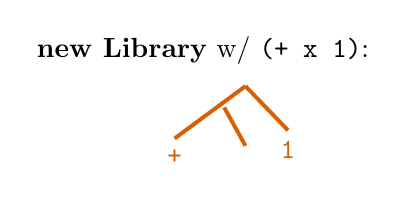
\begin{tikzpicture}[scale=0.9,line width=0.5mm]
          \node[align=center] at (0,0) {\textbf{new Library} w/ \texttt{(+ x 1)}:};
          \begin{scope}[shift={(0.6,-0.5)}]
            \node[pop3](p1) at (-1,-1) {\texttt{+}};
            \node[pop3](n1) at (0.6,-0.9) {\texttt{1}};
            \node[pop3](a) at (0,-1) {\texttt{ }};
            \draw[pop3] (0,0) -- (p1.north);
            \draw[pop3] (0,0) -- (n1.north);
            \draw[pop3] (-0.3,-0.3) -- (a.north);
          \end{scope}
      \end{tikzpicture}};
      \draw [-> ] (c.south) -- (d.north);



      \begin{scope}[shift={(4,-8)},scale=0.6,line width=0.05mm]
        \node[latent,scale=0.7] at (3.5,3) (dx){Library};
        \node[obs,scale=0.7] at ([yshift=-1.7cm,xshift=0cm]dx) (zp){prog};
        \node[obs,scale=0.7] at ([yshift=-1.45cm]zp) (xp) {task};
        \node[obs,scale=0.7] at ([xshift=1.5cm]zp) (zp1){prog};
        \node[obs,scale=0.7] at ([xshift=1.5cm]xp) (xp1) {task};
        \draw [->] (zp1.south) -- (xp1.north);
        \draw [->] (dx.south) -- (zp1.north);
        \node[obs,scale=0.7] at ([xshift=-1.5cm]zp) (zp1){prog};
        \node[obs,scale=0.7] at ([xshift=-1.5cm]xp) (xp1) {task};
        \draw [->] (zp1.south) -- (xp1.north);
        \draw [->] (dx.south) -- (zp1.north);
        \draw [->] (dx.south) -- (zp.north);
        \draw [->] (zp.south) -- (xp.north);
      \end{scope}


      \end{scope}


    
    %% center spiral
    \begin{scope}[shift={(3.25,-7.9)},scale=0.8]    
      \spiral{(3.5,1)}{3.5}
      \node[latent,scale=1] at (3.5,3) (dx){Library};
      \node[latent,scale=1] at ([yshift=-2cm,xshift=0cm]dx) (zp){prog};
      \node[obs,scale=1] at ([yshift=-1.45cm]zp) (xp) {task};
      \node[latent,scale=1] at ([xshift=2cm]zp) (zp1){prog};
      \node[obs,scale=1] at ([xshift=2cm]xp) (xp1) {task};
      \draw [->] (zp1.south) -- (xp1.north);
      \draw [->] (dx.south) -- (zp1.north);
      \draw [->,red] (xp1.east) to[out = 30,in = -30] node(nn){} (zp1.east);
      
      \node[latent,scale=1] at ([xshift=-2cm]zp) (zp1){prog};
      \node[obs,scale=1] at ([xshift=-2cm]xp) (xp1) {task};
      \draw [->] (zp1.south) -- (xp1.north);
      \draw [->] (dx.south) -- (zp1.north);
      \draw [->,red] (xp1.east) to[out = 30,in = -30] node(nn){} (zp1.east);


      \draw [->,red] (xp.east) to[out = 30,in = -30] node(nn){} (zp.east);
      \draw [->] (dx.south) -- (zp.north);
      \draw [->] (zp.south) -- (xp.north);

      \node at ([yshift=-0.6cm]xp.south) {\legend};

    \end{scope}
    
  \end{tikzpicture}
  \caption{\textbf{Middle:} \system as a graphical model. Agent observes programming tasks (e.g., input/outputs for list processing or images for graphics programs), which it explains with latent programs, while jointly inferring a latent library capturing cross-program regularities. A neural network, called the \emph{recognition model} (red arrows) is trained to quickly infer programs with high posterior probability. \textbf{Top}: Wake phase infers programs while holding the library and recognition model fixed. \textbf{Left}: Sleep (Abstraction) phase updates library while holding the programs fixed by refactoring programs found during waking and abstracting out common components (highlighted in orange). \textbf{Right}: Sleep (Dreaming) phase trains recognition model to predict approximate posterior over programs conditioned on task. Trained on `Fantasies' (programs sampled from library) \& `Replays' (programs found during waking).}\label{threeCycles}
\end{figure}



%% Our programs are all
%% strongly typed.  We use the Hindley-Milner polymorphic typing
%% system~\cite{pierce} which is used in functional programming languages
%% like OCaml and Haskell.  We now define DSLs:
%% \begin{definition}
%% A DSL $\mathcal{D}$ is a set of typed $\lambda$-calculus expressions.
%% A weight vector $\theta$ for a DSL $\mathcal{D}$ is a vector of $|\mathcal{D}| + 1$ real numbers:
%% one number for each DSL element $e\in \mathcal{D}$, written $\theta_e$ and controlling the probability of  $e$ occurring in a program,
%% and a weight controlling the probability of a variable occurring in a program, $\theta_{\text{var}}$.
%% \end{definition}
%% \noindent Together with its weight vector, a DSL defines a distribution over
%% programs, $\probability[p|\mathcal{D},\theta]$.  We define this
%% distribution by specifying a procedure for drawing samples from
%% $\probability[p|\mathcal{D},\theta]$ (Appendix~\ref{generativeAppendix}).
%% Care must be taken to ensure that variable scoping rules are obeyed
%% and that programs are well-typed.  We ensure well-typed programs by
%% performing Hindley-Milner type inference~\cite{pierce} during
%% sampling, and assume that each task is annotated with the type of the
%% program that will solve it.
%% Appendix~\ref{enumerationAppendix}
%% explains how we enumerate,
%% rather than sample,
%% programs generated by Algorithm~\ref{sampleProgram}.

%% \begin{comment}

%%   \subsection{Wake: Solving tasks}\label{explorationSection}

%% During waking we enumerate programs from the DSL in decreasing order
%% of their probability according to the recognition model, and then
%% check if a program $p$ assigns positive probability to a task
%% ($\probability[x|p] > 0$); if so, we incorporate $p$ into the beam
%% $\mathcal{B}_x$. We represent programs as polymorphicly-typed
%% $\lambda$-calculus expressions, a representation closely resembling
%% Lisp and functional languages like Haskell and OCaml, including
%% variables, conditionals, higher-order recursive functions, and the
%% ability to create new functions.  We `batch' the tasks by randomly
%% shuffling the training set and playing small minibatches of tasks to
%% the agent during each wake cycle.


%% Why enumerate, when the program synthesis community has invented many
%% sophisticated algorithms that search for programs?~\cite{solar2008program,schkufza2013stochastic,feser2015synthesizing,osera2015type,polozov2015flashmeta}.
%% We have two reasons:
%% (1) A key point of our work is that learning the DSL, along with a neural recognition model, can make program induction tractable, even if the search algorithm is very simple.
%% (2) Enumeration is a general approach that can be applied to any program induction problem. Many of these more sophisticated approaches require special conditions on
%% the space of  programs.
%% \end{comment}
%% \begin{comment}
%%   \begin{figure}
%%     \begin{tikzpicture}[every node/.style={rounded corners,thick}]
%%       \node(x)[draw,align=center] at (0,0) {Task $x$\\e.g., input/outputs};
%%       \node(e)[draw, align=center] at ([xshift=3cm]x.east) {Domain-specific encoder\\
%%         e.g., RNN or CNN};
%%       %    \node(m)[draw,align = center] at ([xshift=1.1cm]e.east) {MLP};%\\Output: $(|\mathcal{D}| + 2)\times(|\mathcal{D}| + 1)\times A$};
%%       \node[draw,align = center](s) at ([xshift=2cm]e.east) {Enumerate\\(Algorithm~\ref{recognitionSample})};
%%       \node(f)[draw,align = center] at ([xshift=2cm]s.east) {Beam\\$\mathcal{B}_x$};

%%       \draw[->] (x.east) -- (e.west);
%%       \draw[->] (e.east) -- (s.west);
%%       %    \draw[->] (m.east) -- node(p)[fill=white,align=center,midway,inner sep=0,outer sep=0,rotate=90]{\small $Q_{ijk}(x)$}(s.west);
%%       \draw[->] (s.east) -- (f.west);
%%       \draw[->] (x.north) -- ([yshift=15]x.north) -- node[above = 0pt,midway]{\small likelihood $\probability[x|p]$}([yshift=15,xshift=40]s.north) -- ($(s.east)!0.5!(f.west)$);
%%       \node[align=center] at ($(0,-1) + (e.center)$) {$\underbrace{\hspace{4cm}}_{\normalsize\text{\normalsize Recognition model $Q(p|x)$}}$};
%%       \node[align=center] at ($(s.west)!0.5!(f.east) + (0,-1)$) {$\underbrace{\hspace{5cm}}_{\text{\normalsize Search}}$};
%%     \end{tikzpicture}
%%     \caption{Neurally-guided program inference pipeline. Recognition model outputs distribution over program $Q(p|x)$. Program output by enumerative search incorporated into beam if likelihood $\probability[x|p] > 0$}
%%     \label{neuralPipeline}
%%   \end{figure}
%% \end{comment}

%%   However, a drawback of   enumerative search  is that we have no
%% efficient means of solving for arbitrary constants that might occur in a
%% program. In Sec.~\ref{regressionSection},
%% we will show how to find programs with real-valued constants
%% by automatically differentiating through the program and setting the constants using gradient descent.
%% In Sec.~\ref{textSection}
%% we will show that the bottom-up neural recognition model can learn
%% which discrete constants should be included in a program.




\subsection{Abstraction Sleep: Growing a Library of Concepts}\label{consolidationSection}

The library offers a set of abstractions that allow an agent to concisely
express solutions to the tasks at hand. We automatically discover
these new abstractions by combining two ideas. First, we build on
techniques from the programming languages community to develop a new
algorithm for automatically refractoring programs, where this
refactoring exposes common reused subexpressions across the
programs found during waking.  Second, we use this automatic refactoring
process to search for libraries that maximally compress these programs by
incorporating reused subexpressions into the library.

Mathematically this compression takes the form of
finding the library maximizing $\int \probability[\mathcal{D},\theta]\probability[X|\mathcal{D},\theta]\;\mathrm{d}\theta$ (Sec.~\ref{overviewSection}).
We replace this marginal with an AIC approximation~\cite{akaike1998information}
and marginalize over refactorings of programs found during waking, minimizing the following expression,
which can be interpreted as a kind of compression:
\begin{equation}
\underbrace{-\log \probability[\mathcal{D}] + \min_{\substack{\theta\\\\\\\\}}\Bigg(-\log
\probability[\theta|\mathcal{D}] + \|\theta\|_0}_{\text{Description length of }(\mathcal{D},\theta)} +\sum_{x\in
  X}\underbrace{-\log \sum_{\substack{p \text{ a refactoring of } p'\\ p'\text{ found during waking}}}\probability[x|p]\probability[p|\mathcal{D},\theta]}_{\text{Description length of programs for task }x}\Bigg)
\label{AIC}
\end{equation}
But a program has infinitely many possible refactorings, rendering
Eq.~\ref{AIC} intractable.  Rather than consider every refactoring we
bound the number of $\lambda$-calculus evaluation steps separating a
program from its refactoring.  Now the number of refactorings is
finite but astronomically large: Figure~\ref{mapFactor}A diagrams a
problem where the agent rediscovers the higher-order function
\code{map} starting from the basics of Lisp and the Y-combinator, but
where there are approximately $10^{14}$ possible refactorings -- a quantity
that grows exponentially both as a function of program size and a
function of the bound on evaluation steps. How can we tame this
combinatorial explosion?

To resolve this exponential growth we introduce a new data structure
combining ideas from version space
algebras~\cite{lau2001programming,mitchell1977version,polozov2015flashmeta}
and equivalence graphs~\cite{tate2009equality}. A version space is a
tree-shaped data structure that compactly represents a large set of
programs and supports efficient set operations like union,
intersection, and membership checking, while equivalence graphs are
data structures that track semantic equivalences between program
subexpressions.  In Appendix~\ref{appendixVersion}, we give a dynamic
program that takes as input a program and then outputs a version space
containing its refactorings while tracking semantically equivalent
subexpressions. Figure~\ref{mapFactor}B diagrams a subtree of a
version space containing refactorings of a small program. Our
technique is substantially more efficient than explicitly representing
the space of possible refactorings: for the example in
Figure~\ref{mapFactor}A, we represent the space of refactorings using
a version space with $10^6$ nodes, which encodes $10^{14}$
refactorings. Appendix~\ref{appendixCompression} specifies how we
combine this probabilistic and symbolic machinery to update the library.
At a high level, our approach is to search locally through the space
of libraries, proposing small changes until Eq.~\ref{AIC} fails to
decrease.




%% However, there is a snag with this simple approach:
%% whenever we add a new expression $e$ to the DSL,
%% the programs found during waking
%% are not written in terms of $e$ ---
%% and so we must \emph{refactor}
%% the programs in terms of the new DSL component.
%% Concretely, imagine we wanted to discover a new DSL procedure for doubling numbers,
%% after having found the programs
%% \code{(cons (+ 9 9) nil)} and \code{($\lambda$ (x) (+ (car x) (car x)))}.
%% As human programmers,
%% we can look at these pieces of code and recognize that,
%% if we define a new procedure called \code{double},
%% defined as \code{($\lambda$ (x) (+ x x))},
%% then we can rewrite the original programs as
%% \code{(cons (double 9) nil)} and \code{($\lambda$ (x) (double (car x)))}.
%% This process is a kind of refactoring
%% where a new subroutine is defined (\code{double})
%% and the old programs rewritten
%% in terms of the new subroutine.
%% Figure~\ref{mapFactor}A diagrams a refactoring process where the agent
%% must rediscover the higher-order function \code{map} starting from the
%% basics of Lisp and the Y-combinator.

%% We refine our objective to compress
%% \emph{refactorings} of the programs found during waking, minimizing
%% \begin{equation}
%%         -\log \probability[\mathcal{D}] + 
%% \min_{\theta}\Bigg(-\log \probability[\theta|\mathcal{D}] + \|\theta\|_0 +\sum_{x\in X} - \log \underbrace{\sum_{\substack{p:\\\exists p'\in \mathcal{B}_x: p\manyReduce p'}}}_{\text{Refactors }\mathcal{B}_x}\probability[x|p]\probability[p|\mathcal{D},\theta]\Bigg)
%% \label{factorObjective}
%% \end{equation}
%% where $p\manyReduce p'$ is the standard notation for ``expression $p$
%% evaluates to $p'$ by the rules of $\lambda$-calculus''~\cite{pierce}.
%% Equation~\ref{factorObjective} captures the idea that we want to add
%% new components to the DSL while jointly refactoring our old programs
%% in terms of these new components.  But this joint optimization is
%% intractable, because there are infinitely many ways of refactoring a
%% program.  To make refactoring tractable we first limit the degree to
%% which a piece of code can be refactored: rather than consider every
%% refactoring, we bound the number of $\lambda$-calculus evaluation
%% steps separating a refactoring from its original program.  Now the
%% number of refactoring this is finite but astronomically large: for the
%% example in Figure~\ref{mapFactor} there are approximately $10^{14}$
%% possible refactorings -- a quantity that grows exponentially both as a
%% function of program size and a function of the bound on evaluation
%% steps. How can we tame this combinatorial explosion?











%% \textbf{Idea 1:} Limit the degree to which
%% a piece of code can be refactored.
%% Instead of considering every refactoring,
%% bound the number of $\lambda$-calculus evaluation steps
%% separating a refactoring from its original program.
%% Formally,
%% we define the set of $n$-step refactorings as:
%% \begin{equation}
%%   R_n(p) = \left\{p'\;:\;p'\underbrace{\reduce p''\reduce\cdots\reduce}_{\text{$\leq n$ times}} p \right\}
%% \end{equation}
%% where $p_1\reduce p_2$ is the standard notation for ``$p_1$ rewrites to $p_2$
%% in one step according to the rules of $\lambda$-calculus''~\cite{pierce}.
%% For example,
%% \begin{align*}
%%   \code{((lambda (x) (x x)) (lambda (y) y))}\reduce&\\
%%   \code{((lambda (y) y) (lambda (y) y))}\reduce&\\
%%   \code{(lambda (y) y)}&
%% \end{align*}
%% Returning to Equation~\ref{factorObjective},
%% this approximation gives the following objective:
%% \begin{equation}
%%         \log \probability[\mathcal{D}] + \argmax_{\theta}\Bigg(\log \probability[\theta|\mathcal{D}] - \|\theta\|_0 +\sum_{x\in X}\log \sum_{p\in \mathcal{B}_x}\probability[x|p]\max_{p'\in R_n(p)}\probability[p'|\mathcal{D},\theta]\Bigg)
%% \label{limitedObjective}
%%   \end{equation}
%% In practice, setting the number of refactoring steps $n$ to 3 suffices
%% to give a competent DSL learning algorithm.  Although the number of
%% refactorings is now finite, it is still prohibitively large, and in
%% fact grows exponentially quickly both as a function of $n$ and as a
%% function of the size of the program being refactored.  For example,
%% for the programs in Figure~\ref{mapFactor}, there are approximately
%% $10^{14}$ possible refactorings.  Next, we show how to tame this
%% exponential explosion.



%% In Appendix~\ref{appendixVersion}, we describe a dynamic program for
%% efficiently constructing a version space containing every $n$-step
%% refactoring.
%% This dynamic program, which we call $I\beta_n(p)$,
%% satisfies $\denotation{I\beta_n(p)} =  R_n(p)$.
%% In other words,
%% this dynamic program
%% builds a data structure
%% that represents the entire set of
%% refactorings -- but without having to explicitly enumerate all of the refactorings.




\begin{figure*}
  \centering\begin{tikzpicture}[every node/.style={inner sep=1,outer sep=0,rounded corners,thick}]
  \node(p1)[draw,rounded corners,thick] at (-1,0) {
    \begin{tabular}{l}
      \texttt{(Y ($\lambda$ (r l) (if (nil? l) nil}\\
      \texttt{ (cons (+ (car l) (car l))}\\
      \phantom{\texttt{(cons }}\texttt{ (r (cdr l))))))}
    \end{tabular}
  };
  \node(r1)[draw,inner sep=0,outer sep=0] at ([yshift=-2.5cm]p1.south) {
    \begin{tabular}{l}
      \texttt{(}\orange{\texttt{($\lambda$ (f) (Y ($\lambda$ (r l) (if (nil? l)}}\\
      \phantom{(($\lambda$ (f) (Y ($\lambda$ (r l)}\orange{\texttt{nil}}\\
      \phantom{(($\lambda$ (f) (Y ($\lambda$ (r l)}\orange{\texttt{(cons (f (car l))}}\\
      \phantom{(($\lambda$ (f) (Y ($\lambda$ (r l)}\orange{\texttt{ (r (cdr l)))))))}}\\
      \texttt{ ($\lambda$ (z) (+ z z)))}
    \end{tabular}
  };

  \node(p2)[draw] at ([xshift=4.5cm]p1.east) {
    \begin{tabular}{l}
      \texttt{(Y ($\lambda$ (r l) (if (nil? l) nil}\\
      \texttt{ (cons (- (car l) 1)}\\
      \phantom{\texttt{(cons }}\texttt{ (r (cdr l))))))}
    \end{tabular}
    
  };
  \node(r2)[draw] at ([yshift=-2.5cm]p2.south) {
    \begin{tabular}{l}
      \texttt{(}\orange{\texttt{($\lambda$ (f) (Y ($\lambda$ (r l) (if (nil? l)}}\\
      \phantom{(($\lambda$ (f) (Y ($\lambda$ (r l)}\orange{\texttt{nil}}\\
      \phantom{(($\lambda$ (f) (Y ($\lambda$ (r l)}\orange{\texttt{(cons (f (car l))}}\\
      \phantom{(($\lambda$ (f) (Y ($\lambda$ (r l)}\orange{\texttt{ (r (cdr l)))))))}}\\
      \texttt{ ($\lambda$ (z) (- z 1)))}
    \end{tabular}

  };

  \draw [->] (p1.south)  --(r1.north) node[fill=white,midway,align=center] {refactor\\($\approx 10^{14}$ refactorings)};
  \draw [->] (p2.south)  --(r2.north) node[fill=white,midway,align=center] {refactor\\($\approx 10^{14}$ refactorings)};

  \node[draw](m) at (3,-6.5) {
    \begin{tabular}{l}
      \fbox{\textsc{map}} = \orange{\texttt{($\lambda$ (f) (Y ($\lambda$ (r l) (if (nil? l) nil}}\\
      \phantom{\texttt{\emph{map}} = \texttt{($\lambda$ (f) (Y ($\lambda$ (r l) (if }}\orange{\texttt{(cons (f (car l))}}\\
      \phantom{\texttt{\emph{map}} = \texttt{($\lambda$ (f) (Y ($\lambda$ (r l) (if }}\orange{\texttt{(r (cdr l))))))}}\\
      \code{(}\fbox{\textsc{map}}\code{ ($\lambda$ (z) (+ z z)))}\quad(program rewritten w/ new \fbox{\textsc{map}} primitive)\\
      \code{(}\fbox{\textsc{map}}\code{ ($\lambda$ (z) (- z 1)))}\quad(program rewritten w/ new \fbox{\textsc{map}} primitive)\\
    \end{tabular}      
  };
  \draw [->](r1.south)--(m.north);
  \draw [->](r2.south)--(m.north);
  \node[fill=white] at ([yshift=0.5cm]m.north) {\textbf{Compress (MDL/Bayes objective)}};

  \node(t1)[draw] at ([yshift=1.5cm]p1.north) {\begin{tabular}{ll}
      \textbf{Task}:&\texttt{(1 2 3)$\to$(2 4 6)}\\
      &\texttt{(4 3 4)$\to$(8 6 8)}
  \end{tabular}};
  \draw [->] (t1.south)  --(p1.north) node[fill=white,midway] {Wake: program search};
  \node(t2)[draw] at ([yshift=1.5cm]p2.north) {\begin{tabular}{ll}
      \textbf{Task}:&\texttt{(1 2 3)$\to$(0 1 2)}\\
      &\texttt{(4 3 4)$\to$(3 2 3)}
  \end{tabular}};
  \draw [->] (t2.south)  --(p2.north) node[fill=white,midway] {Wake: program search};

  \node(panelA)[ultra thick, rounded corners=0, inner sep=10,outer sep=10, draw, fit=(t1) (t2) (m) (r1) (r2)] {}; \node at ($(0.5,0) + (panelA.west |- panelA.north)$) {\textbf{A}};

  \footnotesize
  \begin{scope}[shift={(-1,-12)}]  
    \node[draw, rounded corners](u1) at (0,0) {union};
    \node[draw, rounded corners](u2) at ($(0,-1) + (u1.south)$) {\code{(}union\code{ 1)}}; \draw (u1.south) -- (u2.north);
    \node[draw, rounded corners](u21) at ($(-1.3,-1) + (u2.south)$) {\code{(($\lambda$ (x) (x 1)) +)}}; \draw ([xshift=-0.2cm]u2.south) -- (u21.north);
    \node[draw, rounded corners](u22) at ($(2.3,-1) + (u2.south)$) {\code{(($\lambda$ (x) (+ x)) 1)}};  \draw ([xshift=-0.2cm]u2.south) -- (u22.north);

    \node[draw, rounded corners](u11) at ($(-1.75,-1) + (u1.south)$) {\code{(+ 1 1)}}; \draw (u1.south) -- (u11.north);
    \node[draw, rounded corners](u12) at ($(2.75,-1) + (u1.south)$) {\code{(($\lambda$ (x) (x 1 1)) +)}}; \draw (u1.south) -- (u12.north);

    \node(vs) at ($(u21.west)!0.5!(u12.east) + (0,-1.25)$) {$\underbrace{\hspace{8cm}}_{\text{\normalsize Subset of version space}}$};

    \node[anchor=north](p) at ($(0,2.5) + (u1)$) {\normalsize Program: \texttt{(+ 1 1)}};
    \draw[ultra thick,->] ($(0,-0.1) + (p.south)$) --node[sloped, above, inner sep=5]{Refactors} ($(0,0.1) + (u1.north)$);
    \node(g)[anchor=left] at ($(7,0) + (u12.east)$) {\includegraphics[width = 6cm]{figures/vs.eps}};
    \node(panelB)[ultra thick, rounded corners=0, inner sep=10,outer sep=10, draw, fit=(p) (u1) (vs) (g)] {}; \node at ($(0.5,0) + (panelB.west |- panelB.north)$) {\normalsize\textbf{B}}; 


    %% \node(panelC)[ultra thick, rounded corners=0, inner sep=8,outer sep=8, draw, fit=(g)] {}; \node at ($(0.5,0) + (panelC.west |- panelC.north)$) {\normalsize\textbf{C}}; 
  \end{scope}
  
  \end{tikzpicture}
  \caption{Library learning as code refactoring. \textbf{Panel A:} During waking we discover programs for each task, then refactor the code from those programs to expose common subprograms (highlighted in \orange{orange}). Common subprograms are incorporated into the library when they increase a Bayesian objective. Intuitively, these new components best compress the programs found during waking. \textbf{Panel B:} \# of possible refactorings grows exponentially with program size, so we represent refactorings using version spaces, which augment syntax trees with a \emph{union} operator whose children are themselves version spaces. Right graph: version spaces are exponentially more efficient than explicitly constructing set of refactorings. In this graph, refactored programs are of the form $1+1+\cdots  + 1$.}\label{mapFactor}
\end{figure*}


\subsection{Dream Sleep: Training a Neural Recognition Model}\label{recognitionSection}

During ``dreaming'' the system learns a recognition model that guides
program search.  It learns from (program, task) pairs drawn from two
sources of self-supervised data: \emph{replays} of programs discovered
during waking, and \emph{fantasies}, or programs drawn from $(\mathcal{D},\theta)$.
Replays ensure that the recognition model is trained on the actual
tasks it needs to solve, and does not forget how to solve them.
Fantasies ensure that the recognition model has a large and highly
varied corpus of (program, task) pairs to learn from.

Formally, the recognition model $Q(p|x)$ should approximate the posterior
$\probability[p|\mathcal{D},\theta,x]$.
We can either train $Q$ to perform full posterior inference by minimizing the expected KL-divergence, $  \expect\left[\text{KL}\left(\probability[p|x,\mathcal{D},\theta]\|Q(p|x) \right) \right]$,
or we can train $Q$ to perform MAP inference
by maximizing $\expect\left[\max_{p\text{ maxing }\probability[\cdot |x,\mathcal{D},\theta]} \log Q(p|x) \right]$,
where in both cases the expectation is taken over tasks. Taking this expectation over the empirical distribution of tasks trains $Q$ on replays; taking it over samples from the generative model trains $Q$ on fantasies.
We define a pair of alternative objectives for the recognition model,
$\mathcal{L}^{\text{posterior}}$ and $\mathcal{L}^{\text{MAP}}$,
which either train $Q$ to perform full posterior inference or MAP inference, respectively.
These objectives combine replays and fantasies:
\begin{align*}
  \mathcal{L}^{\text{posterior}} &= \mathcal{L}_{\text{Replay}}^{\text{posterior}} + \mathcal{L}_{\text{Fantasy}}^{\text{posterior}}&
  \mathcal{L}^{\text{MAP}} &= \mathcal{L}_{\text{Replay}}^{\text{MAP}} + \mathcal{L}_{\text{Fantasy}}^{\text{MAP}}\\
  \mathcal{L}_{\text{Replay}}^{\text{posterior}}& = \expect_{x\sim X}\left[\sum_{p\in \mathcal{B}_x}
    \frac{\probability\left[x,p|\mathcal{D},\theta \right]\log Q(p|x)}{\sum_{p'\in \mathcal{B}_x}\probability\left[x,p'|\mathcal{D},\theta \right]}\right] &
  \mathcal{L}_{\text{Replay}}^{\text{MAP}}& = \expect_{x\sim X}\left[\max_{\substack{p\in \mathcal{B}_x\\p\text{ maxing }\probability[\cdot |x,\mathcal{D},\theta]}} \log Q(p|x) \right]  \\
  \mathcal{L}_{\text{Fantasy}}^{\text{posterior}} &= \expect_{(p,x)\sim(\mathcal{D},\theta) }\left[\log Q(p|x)\right]&
  \mathcal{L}_{\text{Fantasy}}^{\text{MAP}} &= \expect_{x\sim(\mathcal{D},\theta) }\left[\max_{\substack{p\\p\text{ maxing }\probability[\cdot |x,\mathcal{D},\theta]}}\log Q(p)\right]
\end{align*}
We maximize $\mathcal{L}^{\text{MAP}}$ rather than
$\mathcal{L}^{\text{posterior}}$ for two reasons:
$\mathcal{L}^{\text{MAP}}$ prioritizes the shortest program solving a
task, thus more strongly accelerating enumerative search during waking;
and, combined with our parameterization of $Q$, described next, we
will show that $\mathcal{L}^{\text{MAP}}$ forces the recognition model
to break symmetries in the space of programs.

\noindent\textbf{Parameterizing $Q$.} The recognition model predicts a
fixed-dimensional tensor encoding a distribution over routines in
the library, conditioned on the local context in the syntax tree of the
program. This local context consists of the parent node in the syntax
tree, as well as which argument is being generated, functioning as a
kind of `bigram' model over trees. Figure~\ref{symmetry} (left)
diagrams this generative process.  This parameterization confers three
main advantages: (1) it supports fast enumeration and sampling of
programs, because the recognition model only runs once per
task, like in~\cite{balog2016deepcoder,ecc,menon2013machine} -- thus
we can fall back on fast enumeration if the target program is unlike
the training programs; (2) the recognition model provides fine-grained
information about the structure of the target program, similar
to~\cite{devlin2017robustfill,zavershynskyi2018naps}; and (3) in
conjunction with $\mathcal{L}^{\text{MAP}}$ the recognition model
learns to break symmetries in the space of programs.

\noindent\textbf{Symmetry breaking.} Effective domain-specific representations not only exposes high-level building blocks, but also
carefully restrict the ways in which those building blocks are
allowed to compose.  For example,
%% a DSL for list manipulation should
%% contain both the empty list and a routine for appending lists, but
%% should not allow appending the empty list.  Similarly 
when searching over arithmetic expressions, one could disallow adding zero, and force
right-associative addition. A bigram parameterization of the recognition
model, combined with the $\mathcal{L}^{\text{MAP}}$ training
objective, interact in a way that breaks symmetries like these, allowing the agent to more efficiently explore the space of
programs.  This interaction occurs because the bigram parameterization
can disallow library routines depending on their local syntactic
context, while the $\mathcal{L}^{\text{MAP}}$ objective forces all
probability mass onto a single member of a set of syntactically
distinct but semantically equivalent expressions
(Appendix~\ref{recognitionAppendix}).
We experimentally confirm this symmetry-breaking
behavior by training recognition models that minimize either
$\mathcal{L}^{\text{MAP}}$/$\mathcal{L}^\text{posterior}$ and which
use either a bigram parameterization/unigram\footnote{In the unigram variant $Q$ predicts a $|\mathcal{D}| + 1$-dimensional vector: $Q(p|x) = \probability[p|\mathcal{D},\theta_i = Q_i(x)]$,
  and was used in our prior work~\cite{ecc}} parameterization.
Figure~\ref{symmetry} (right) shows the result of training $Q$ in these four regimes
and then sampling programs.
On this particular run,
the combination of
bigrams and $\mathcal{L}^{\text{MAP}}$ learns to
avoid adding zero and associate addition to the right ---
different random initializations
lead to either right or left association.




%% \subsubsection{Parameterizing $Q$}\label{recognitionParameterization}

%% Broadly the literature contains two different approaches to
%% parameterizing conditional distributions over programs.  The first
%% approach~\cite{devlin2017robustfill,zavershynskyi2018naps} is to use a
%% recurrent network to predict the entire program token-by-token, which
%% has the advantage that, if the network is sufficiently powerful, it
%% can completely solve the synthesis problem.  The disadvantage is that
%% these models can perform poorly at out-of-sample
%% generalization~\cite{}, which is critical for our setting, as the
%% agent may need to solve new tasks that are qualitatively different
%% from the tasks it has solved so far.

%% %% Second, a powerful deep
%% %% recurrent network may be costly to sample or enumerate from --- so if
%% %% the network cannot easily solve a task, we cannot compensate with
%% %% rapid sampling or enumeration.  In contrast, state-of-the-art
%% %% enumerative program synthesizers evaluate millions of programs per
%% %% second~\cite{feser2015synthesizing}.

%% The second approach is to have $Q$ predict a fixed-dimensional weight
%% vector, which then biases a fast enumerator~\cite{balog2016deepcoder,ecc}
%% or sampler~\cite{menon2013machine}.  This approach can enjoy strong
%% out-of-sample generalization, because it can fall back on enumeration
%% or sampling when the target program is unlike the training programs.
%% A main drawback is that the neural net is deliberately handicapped,
%% and can only send so much information about the target program.

%% We adopt a middle ground between these two extremes.  Our recognition
%% model predicts a distribution over primitives in the DSL,
%% conditioned on the local context in the syntax tree of the
%% program. When predicting the next node to add to the syntax tree of a program,
%% the recognition model
%% conditions on the parent node, as well as
%% which argument is being generated.
%% This is a kind of `bigram' model over trees,
%% where the bigrams
%% take the form of (parent, child, argument index).
%% Figure~\ref{symmetry} (left) diagrams this generative process and Algorithm~\ref{recognitionSample}
%% specifies a sampling procedure for $Q(\cdot |x)$.
%% This parameterization
%% confers three main advantages:
%% (1) it supports fast enumeration
%% and sampling of programs,
%% because the
%% recognition model
%% only needs to run once for each task;
%% (2) it allows the recognition model to provide fine-grained
%% information about the structure of the target program;
%% and (3)
%% training this recognition model
%% causes it to learn to break symmetries in the space of programs,
%% described next.

%% \subsubsection{Learning to break symmetries in program space}\label{symmetricSection}

%% A good DSL not only exposes high-level building blocks, but also
%% carefully restricts the ways in which those building blocks are
%% allowed to compose.  For example,
%% %% a DSL for list manipulation should
%% %% contain both the empty list and a routine for appending lists, but
%% %% should not allow appending the empty list.  Similarly 
%% a DSL for arithmetic should contain both addition and the number zero
%% but disallow adding zero.  These restrictions break symmetries in the
%% space of programs.  A bigram parameterization of the recognition
%% model, combined with the $\mathcal{L}^{\text{MAP}}$ training
%% objective, interact in a way that breaks symmetries in the program
%% space, allowing the agent to more efficiently explore the space of
%% programs.  This interaction occurs because the bigram parameterization
%% can disallow DSL primitives depending on their local syntactic
%% context, while the $\mathcal{L}^{\text{MAP}}$ objective forces all
%% probability mass onto a single member of a set of syntactically
%% distinct but semantically equivalent expressions
%% (Appendix~\ref{recognitionAppendix}).




%% We experimentally confirm this symmetry-breaking
%% behavior by training recognition models that minimize either
%% $\mathcal{L}^{\text{MAP}}$/$\mathcal{L}^\text{posterior}$ and which
%% use either a bigram parameterization/unigram\footnote{In the unigram variant $Q$ predicts a $|\mathcal{D}| + 1$-dimensional vector: $Q(p|x) = \probability[p|\mathcal{D},\theta_i = Q_i(x)]$,
%%   and was used in our prior work~\cite{ecc}} parameterization.
%% Figure~\ref{symmetry} shows the result of training $Q$ in these four regimes for a DSL containing \code{+}, \code{0}, and \code{1}
%% and then sampling programs.
%% On this particular run,
%% the combination of
%% bigrams and $\mathcal{L}^{\text{MAP}}$ learns to
%% avoid adding zero and associate addition to the right ---
%% different random initializations
%% lead to either right or left association.

\begin{figure}
  \begin{minipage}[c]{0.3\textwidth}
    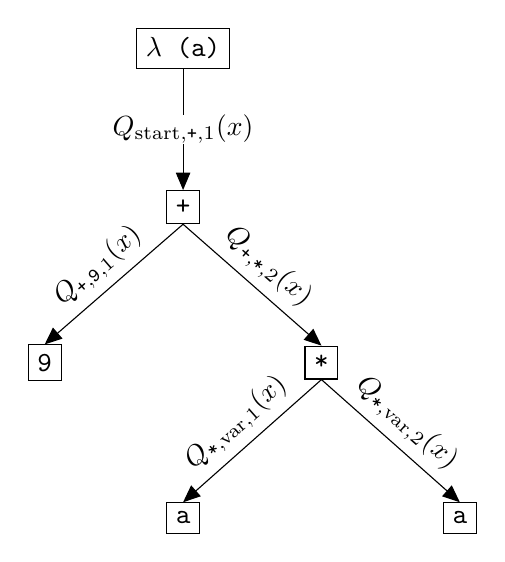
\begin{tikzpicture}[scale=1]%[every node/.style={inner sep=0,outer sep=0}]
    \node(l)[draw] at (0,0) {\texttt{$\lambda$ (a)}};
    \node(k)[draw] at ([yshift=-50]l.south) {\texttt{+}};
    \node(o)[draw] at ([xshift=-50,yshift=-50]k.south) {\texttt{9}};
    \node(m)[draw] at ([xshift=50,yshift=-50]k.south) {\texttt{*}};
    \node(x1)[draw] at ([xshift=50,yshift=-50]m.south) {\texttt{a}};
    \node(x2)[draw] at ([xshift=-50,yshift=-50]m.south) {\texttt{a}};

    \draw[->] (l.south)-- node[fill=white,align=center,midway,inner sep=0,outer sep=0]{$Q_{\text{start},\texttt{+},1}(x)$}(k.north);
    \draw[->] (k.south)--node[sloped, above]{$Q_{\texttt{+},\texttt{9},1}(x)$}(o.north);
    \draw[->] (k.south)--node[sloped, above]{$Q_{\texttt{+},\texttt{*},2}(x)$}(m.north);
    \draw[->] (m.south)--node[sloped, above]{$Q_{\texttt{*},\text{var},2}(x)$}(x1.north);
    \draw[->] (m.south)--node[sloped, above]{$Q_{\texttt{*},\text{var},1}(x)$}(x2.north);
\end{tikzpicture}
    \end{minipage}\hfill%
  \begin{tabular}{cll}
     \toprule
&     \multicolumn{1}{c}{Unigram}&\multicolumn{1}{c}{Bigram} \\\midrule
     \rotatebox[origin=c]{90}{$\mathcal{L}^{\text{posterior}}$}&
     \begin{tabular}{l}
       \emph{Three samples:}\\
       \code{(+ 1 0)}\\
\code{(+ (+ 0 0)}\\\code{\phantom{(+ }(+ 1 0))}\\
\code{(+ 1 1)}
\\
63.0\% right-associative\\37.4\% \code{+0}'s
       \end{tabular}
     &
     \begin{tabular}{l}
       \emph{Three samples:}\\
       \code{0}\\
\code{(+ (+ (+ 0 0)}\\\code{\phantom{(+ (+} (+ 0 1)) 1)}\\
\code{1}\\
55.8\% right-associative\\31.9\% \code{+0}'s
       \end{tabular}
     \\\\
     \rotatebox[origin=c]{90}{$\mathcal{L}^{\text{MAP}}$}&
     \begin{tabular}{l}
       \emph{Three samples:}\\
       \code{1}\\
       \code{(+ 1 (+ 1 (+ (+ 1 }\\\code{\phantom{(+ }(+ 1 1)) 1)))}\\
       \code{(+ (+ 1 1) 1)}
\\48.6\% right-associative\\
       0.5\% \code{+0}'s       
       \end{tabular}
     &
     \begin{tabular}{l}
       \emph{Three Samples:}\\
\code{(+ 1 (+ 1 (+ 1}\\\code{\phantom{(+ 1} (+ 1 (+ 1 1)))))}\\
\code{0}\\
\code{(+ 1 (+ 1 (+ 1 1)))}
       \\
       \textbf{97.9\% right-associative}\\
       2.5\% \code{+0}'s       
       \end{tabular}
\\    \bottomrule 
  \end{tabular}
  \caption{\textbf{Left:} Bigram parameterization of distribution over programs predicted by recognition model.
  Here the program (syntax tree shown above) is \texttt{($\lambda$ (a) (+ 9 (* a a )))}.
Each conditional distribution predicted by the recognition model is written $Q_{\text{parent},\text{child},\text{argument index}}(x)$, where $x$ is a task. \textbf{Right:} Agent learns to break symmetries in program space only when using both bigram parameterization and $\mathcal{L}^{\text{MAP}}$ objective, associating addition to the right and avoiding adding zero. \% right-associative calculated by drawing 500 samples from $Q$. $\mathcal{L}^{\text{MAP}}$/Unigram agent incorrectly learns to never generate programs with \code{0}'s, while $\mathcal{L}^{\text{MAP}}$/Bigram agent correctly learns that \code{0} should only be disallowed as an argument of addition. Tasked with building programs from \code{+}, \code{1}, and \code{0}. }\label{symmetry}
\end{figure}

%% \begin{figure}
%% \centering  \begin{tabular}{cll}
%%      \toprule
%% &     \multicolumn{1}{c}{Unigram}&\multicolumn{1}{c}{Bigram} \\\midrule
%%      $\mathcal{L}^{\text{posterior}}$&
%%      \begin{tabular}{l}
%%        \emph{Three samples:}\\
%%        \code{(+ 1 0)}\\
%% \code{(+ (+ 0 0) (+ 1 0))}\\
%% \code{(+ 1 1)}
%% \\
%% 63.0\% right-associative; 37.4\% \code{+0}'s
%%        \end{tabular}
%%      &
%%      \begin{tabular}{l}
%%        \emph{Three samples:}\\
%%        \code{0}\\
%% \code{(+ (+ (+ 0 0) (+ 0 1)) 1)}\\
%% \code{1}\\
%% 55.8\% right-associative; 31.9\% \code{+0}'s
%%        \end{tabular}
%%      \\\\
%%      $\mathcal{L}^{\text{MAP}}$&
%%      \begin{tabular}{l}
%%        \emph{Three samples:}\\
%%        \code{1}\\
%%        \code{(+ 1 (+ 1 (+ (+ 1 (+ 1 1)) 1)))}\\
%%        \code{(+ (+ 1 1) 1)}
%% \\48.6\% right-associative;
%%        0.5\% \code{+0}'s       
%%        \end{tabular}
%%      &
%%      \begin{tabular}{l}
%%        \emph{Three Samples:}\\
%% \code{(+ 1 (+ 1 (+ 1 (+ 1 (+ 1 1)))))}\\
%% \code{0}\\
%% \code{(+ 1 (+ 1 (+ 1 1)))}
%%        \\
%%        \textbf{97.9\% right-associative};
%%        2.5\% \code{+0}'s       
%%        \end{tabular}
%% \\    \bottomrule 
%%   \end{tabular}
%%   \caption{Agent learns to break symmetries in program space only when using both bigram parameterization and $\mathcal{L}^{\text{MAP}}$ objective, associating addition to the right and avoiding adding zero. \% right-associative calculated by drawing 500 samples from $Q$. $\mathcal{L}^{\text{MAP}}$/Unigram agent incorrectly learns to never generate programs with \code{0}'s, while $\mathcal{L}^{\text{MAP}}$/Bigram agent correctly learns that \code{0} should only be disallowed as an argument of addition. Tasked with building programs from \code{+}, \code{1}, and \code{0}. }\label{symmetry}
%%   \end{figure}



\section{Experiments}

\subsection{Conditional programs that manipulate sequences}\label{sequences}
We first apply \system to two classic benchmark domains: list
processing and text editing. In both cases we solve tasks specified by
a conditional mapping (i.e., input/output examples), starting with a
generic functional programming basis, including routines like
\code{map}, \code{fold}, \code{cons}, \code{car}, \code{cdr}, etc.
%% : \code{foldr}, \code{unfold}, \code{if}, \code{map},
%% \code{length}, \code{index}, \code{=}, \code{+}, \code{-}, \code{0},
%% \code{1}, \code{cons}, \code{car}, \code{cdr}, \code{nil}, and
%% \code{is-nil}.

\subsubsection{List Processing}\label{listSection}
We took 218 list manipulation tasks from our previous work~\cite{ecc},
each with 15 input/output examples.  In solving these tasks, the
system typically composes around 20 new library routines, and discovered multiple
higher-order functions. Each round of abstraction built on
concepts discovered in earlier sleep cycles --- for example the
agent first learns the higher-order function \code{filter}, uses
\code{filter} to learn to take the maximum element of a list, then
uses that routine to learn a new component for extracting the
$n^{\text{th}}$ largest element of a list, which it finally uses to
solve a task involving sorting a list of numbers (Figure~\ref{exampleDSL}).
This incremental, modular learning of deep hierarchies of library
components occurs because of the alternation between code writing
(during waking) and code refactoring (during the abstraction phase
of sleep).

\subsubsection{Text Editing}\label{textSection}
Synthesizing programs that edit text is a classic problem in the
programming languages and AI literatures~\cite{lau2001programming},
and algorithms that synthesize text editing programs ship in Microsoft
Excel~\cite{gulwani2011automatin}.  This prior work uses
hand-engineered libraries of primitives and hand-engineered search strategies.  Here, we
will show that we can jointly learn both these ingredients and surpass
the state-of-the-art domain-general program synthesizers on a standard
text editing benchmark.

%% Because our enumerative search procedure cannot generate string %
%% constants, we instead enumerate programs with string-valued
%% parameters.  For example, to learn a program that prepends ``Dr.'', we
%% enumerate $\text{\code{(}}f_3\code{ string s)}$ -- where $f_3$ is the
%% learned appending primitive (Fig.~\ref{initialExampleDSL}) --- and then
%% define $\probability[x|p]$ by approximately marginalizing out the
%% string parameters via a simple dynamic program.
%% In Sec.~\ref{regressionSection}, we will use a similar trick to
%% synthesize programs containing real numbers, but using gradient
%% descent instead of dynamic programming.

We trained our system on 128 automatically-generated text editing tasks, with 4 input/output examples each.
We tested, but did not train, on the 108 text editing problems from the SyGuS~\cite{alur2016sygus} program synthesis competition. Before any learning,
\system solves 3.7\% of the problems within 10 minutes with an average search time of 235 seconds.
After learning,
it solves 79.6\%, and does so much faster,
solving them in an average of 40 seconds.
As of the 2017 SyGuS competition,
the best-performing synthesizer (CVC4) solves 82.4\% of the problems ---
but here, the competition conditions are 1 hour \& 8 CPUs per problem,
and with this more generous compute budget we
surpass
this previous
result and solve
84.3\% of the problems.
SyGuS additionally comes with a
different hand-engineered libraries of primitives \emph{for each text editing problem}. %\footnote{SyGuS text editing problems also prespecify the set of allowed string constants for each task. For these experiments, our system did not use this assistance.}
Here  we learned a single library of text-editing concepts
that applied generically to
all of the tasks,
and perform comparably to the best
prior work.


\subsection{Generative \& Procedural Programs}
%% We consider three domains where the agent must infer a program from an
%% image (Figure~\ref{visualSpecs}).
%% First we consider programs that make plans and take actions:  drawing pictures and building towers out of blocks (Sec.~\ref{logoSection}-\ref{towerSection}).

\subsubsection{Programs for Smooth Trajectories}\label{regressionSection}
Many procedures that people learn, like as motor routines, can be
thought of as some kind of smooth trajectory. Modeling these
procedures as programs entails jointly inferring their combinatorial
structure and their continuous parameters.  We consider simple
programs generating trajectories described by polynomials (up to
degree 4) and rational functions, and equip our learner with a
primitive for introducing a continuous parameter into the discrete
structure of its programs, which an inner loop optimizes via gradient
descent. We penalize the use of real-valued parameters using a
BIC~\cite{Bishop:2006:PRM:1162264} likelihood model.  We use a convolutional neural
network as a `visual' recognition model, which observes a graph of the
trajectory over time, allowing the agent to `eyeball' the trajectory
prior to writing code that describes it
(Figure~\ref{symbolicRegressionExamples}).  In solving 100 such tasks,
the model learns to find programs minimizing the number of continuous
parameters --- this phenomenon arises from our Bayesian framing: both
the generative model's bias toward shorter programs, and the likelihood
model's BIC penalty.
\begin{figure}[b]
    \includegraphics[width = \textwidth]{figures/sr16_horizontal.png}
  \caption{Sixteen smooth-trajectory tasks. Agent writes a program containing continuous real numbers that fits the points along the curve. Recognition model is a CNN that takes as input a graph of the trajectory over time (shown above). Task is `solved' if program matches points on curve.}\label{symbolicRegressionExamples}
  \end{figure}
\subsubsection{Programs that generate images}\label{logoSection}

Procedural or generative visual concepts 
--- from Bongard problems~\cite{Moscow}, to handwritten characters~\cite{lake2015human,hofstadter1993letter}, to Raven's progressive
matrices~\cite{raven2003raven} --- are studied across AI and cognitive science.  Here we take
inspiration from LOGO Turtle graphics~\cite{turtle}, tasking our agent
with drawing a corpus of 160 images (Figure~\ref{logoMaster}, top) while equipping it with control
over a `pen', along with arithmetic operations on angles and
distances.

Inside its learned library we find interpretable parametric drawing
routines corresponding to the families of visual objects in its
training data, like polygons, circles, and spirals
(Figure~\ref{logoMaster}, middle) -- without supervision the agent
has learned the basic types of objects in its visual world. It
additionally learns more abstract visual relationships, like
radial symmetry, which it models by abstracting out a new higher-order
function into its library.

What does \system dream of?  Prior to learning random programs written using the library
are simple and largely unstructured (Figure~\ref{logoMaster}, bottom left).
After training the samples become richly structured
(Figure~\ref{logoMaster}, bottom right), compositionally recombining latent
building blocks and motifs acquired from the training data. This
offers a visual window into how the generative model bootstraps recognition
model training: as the library grows more finely tuned to the domain, the
neural net gets richer and more highly varied training data.
\begin{figure}
  \centering
  \begin{tabular}{cc}
\toprule     \multicolumn{2}{c}{    Subset of 160 tasks}\\\midrule
    \multicolumn{2}{c}{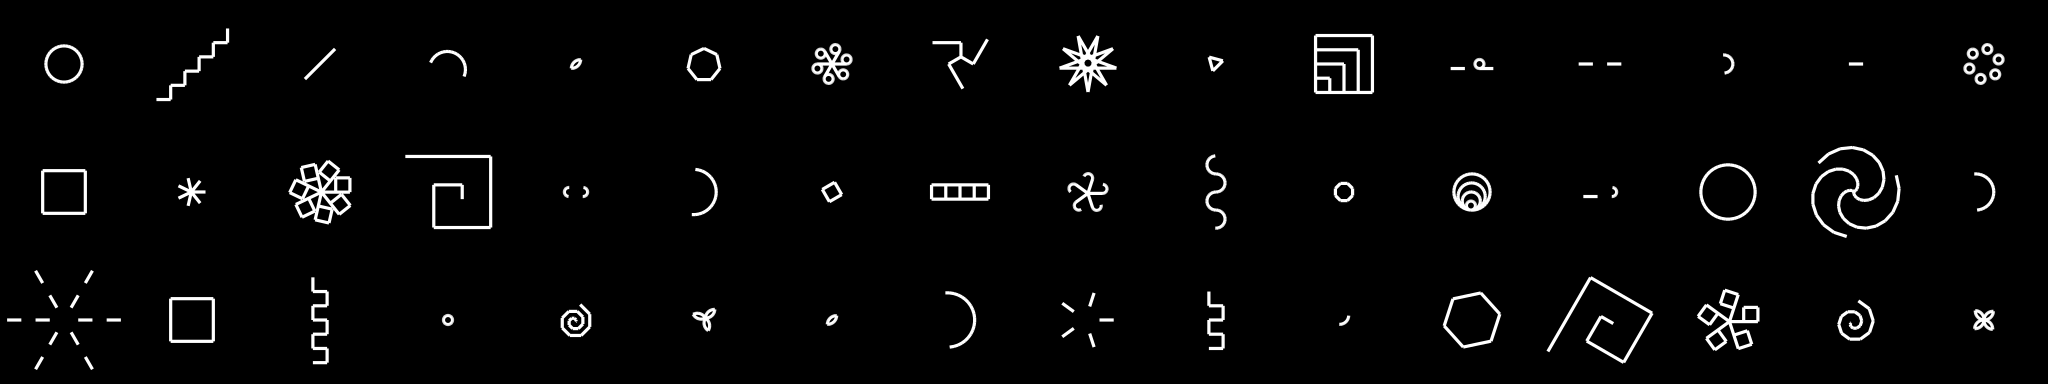
\includegraphics[width = \textwidth]{figures/horizontalLogoTasks.png}}\\\\ 
    

    \midrule  Parametric drawing routines in library&Higher-order drawing routine in library\\\midrule
    \begin{tabular}{rl}
      Semicircle:& \raisebox{-.5\height}{\includegraphics[width = 0.3\textwidth]{figures/logo_primitives/logo_primitive_24.png}}\\
      Circles:
      &\raisebox{-.5\height}{\includegraphics[width = 0.3\textwidth]{figures/logo_primitives/logo_primitive_23.png}}\\
      Spiral:&\raisebox{-.5\height}{\includegraphics[width = 0.3\textwidth]{figures/logo_primitives/logo_primitive_25.png}}\\
      Greek Spiral:&\raisebox{-.5\height}{
\includegraphics[width = 0.3\textwidth]{figures/logo_primitives/logo_primitive_10.png}}\\
      S-Curves:&\raisebox{-.5\height}{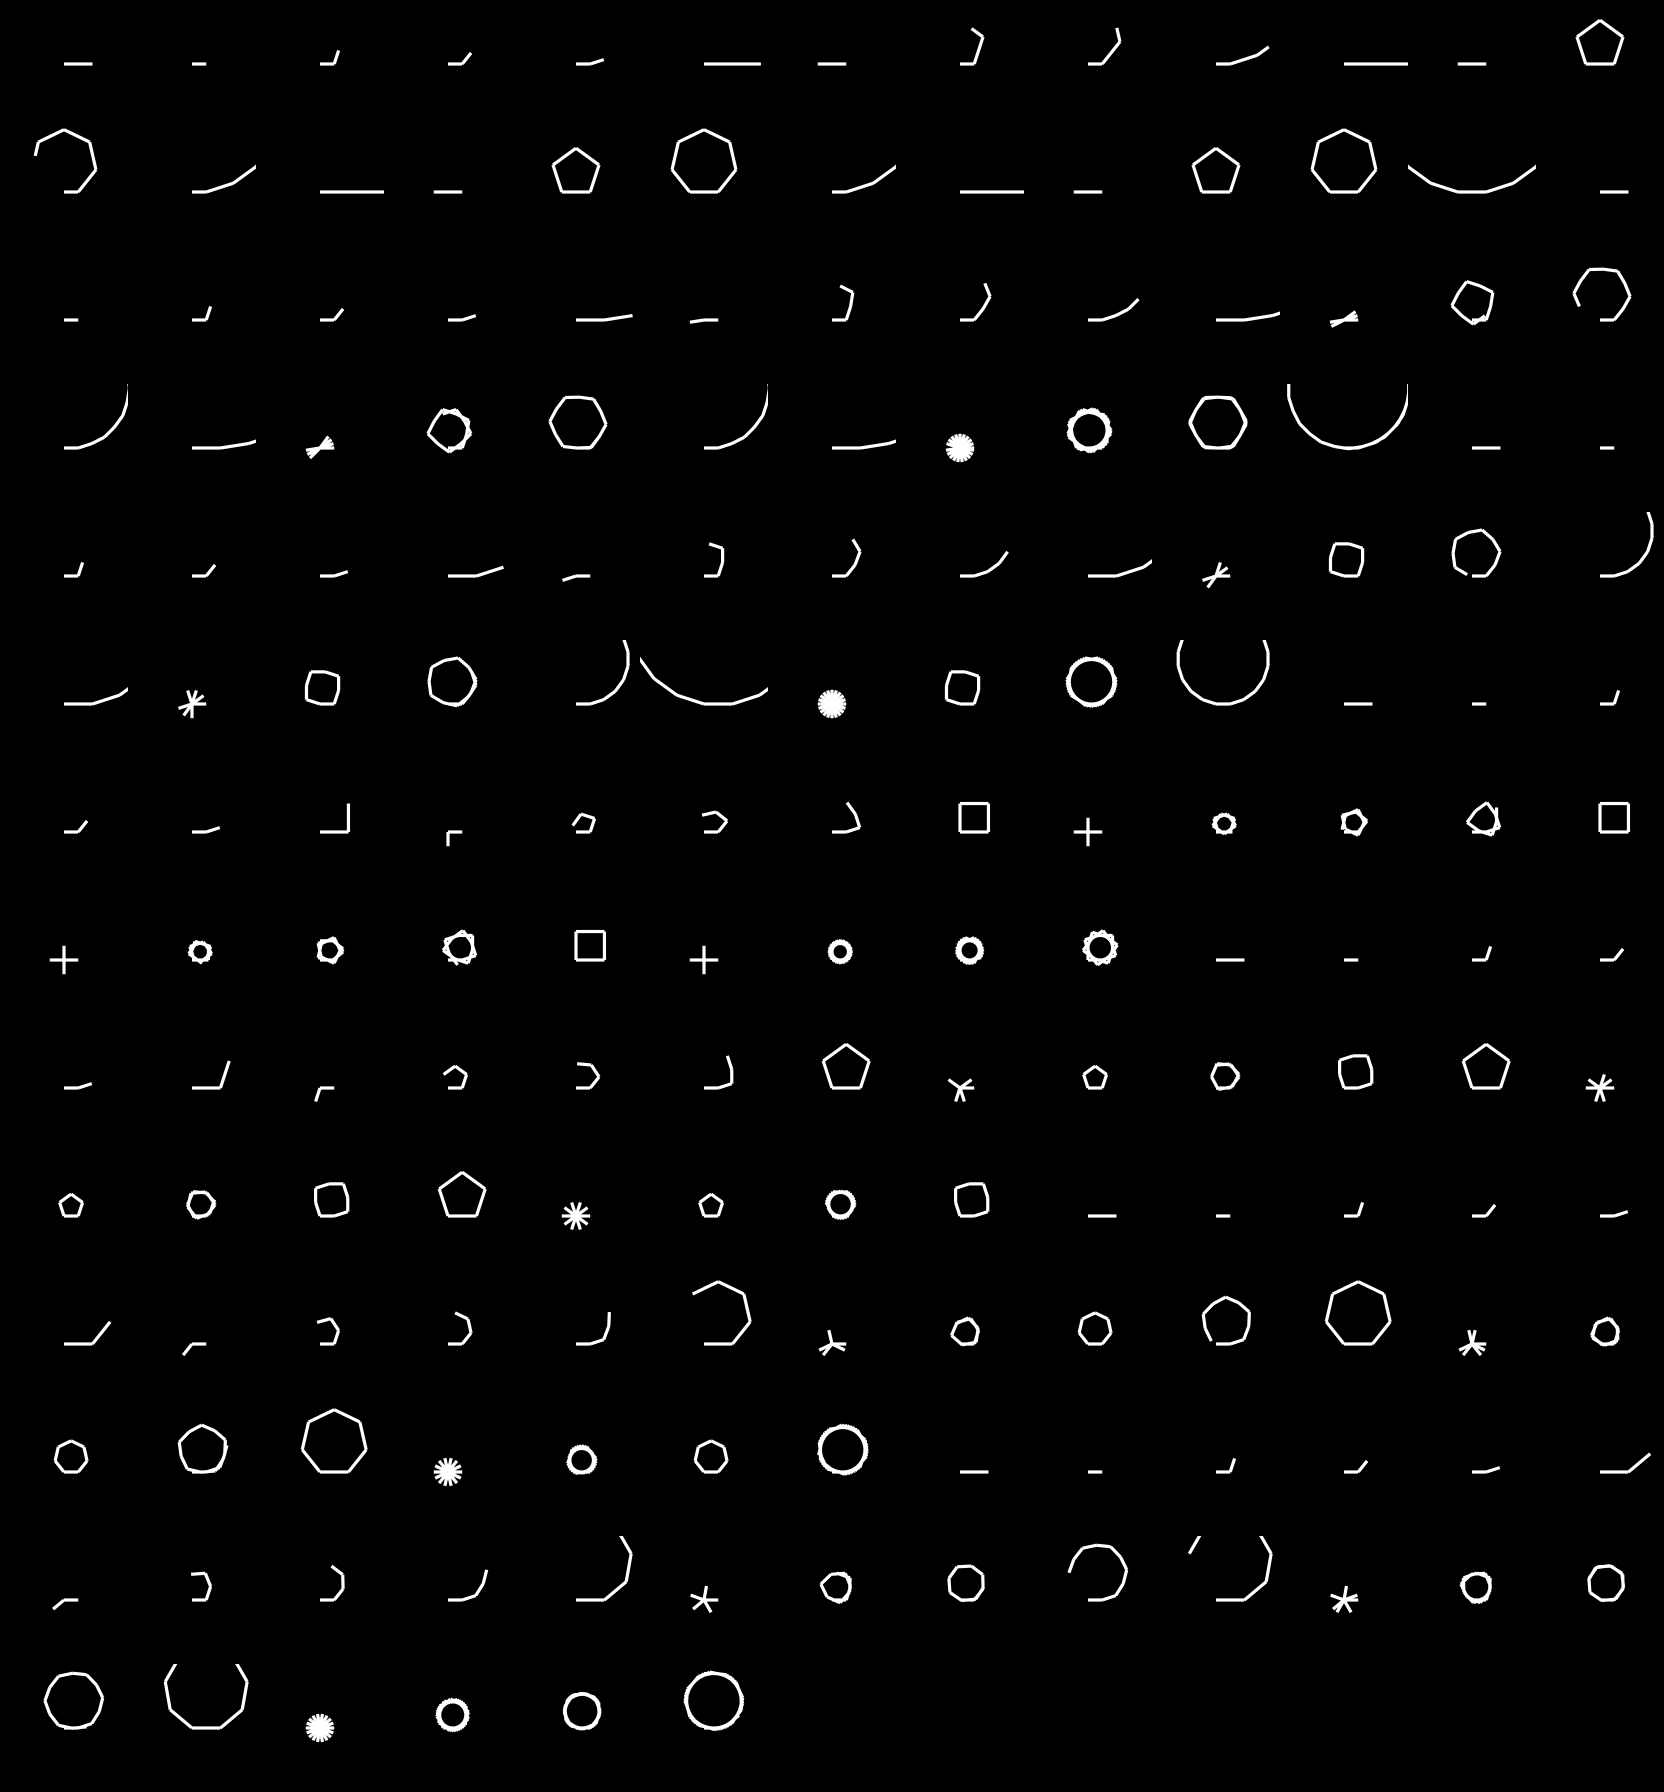
\includegraphics[width = 0.3\textwidth]{figures/logo_primitives/logo_primitive_11.png}}        \\
        Polygons \& Stars:
&\raisebox{-.5\height}{
\includegraphics[width = 0.3\textwidth]{figures/logo_primitives/logo_primitive_12.png}}
    \end{tabular}
    &
    \begin{tabular}{c}
      Radial Symmetry:\\
          \includegraphics[width = 0.35\textwidth]{figures/rotationalmontage.png}
      \end{tabular}
    
    \\\bottomrule \\\\
    \multicolumn{2}{c}{
      \begin{tabular}{ccc}
        Dreams before learning&Dreams after learning&\\
        \begin{tabular}{c}
          \includegraphics[width = 0.4\textwidth]{figures/initialDreams/montage.png}
        \end{tabular}&
        \begin{tabular}{c}
          \includegraphics[width = 0.4\textwidth]{figures/finalDreams/cherry_random_montage.png}
        \end{tabular}&
        \rotatebox[origin=c]{90}{Cherry picked\hspace{2.5cm}Random}
      \end{tabular}
    }
  \end{tabular}
  \caption{\textbf{Top}: 48 (out of 160) LOGO graphics tasks. Agent writes a program controlling a `pen' that draws the target picture. \textbf{Middle}: Example learned library routines. Agent learns parametric routines for drawing families of curves (left) as well as subroutines that take entire programs as input (right). Each row of images on the left is the same code executed with different parameters. Each image on the right is the same code executed with different parameters and with a different subprogram provided as input. \textbf{Bottom}: Sixteen dreams, or sampled programs, from library before (left) and after (right) learning. Blue: where the agent started drawing. Pink: where the agent ended drawing.}\label{logoMaster}
  \end{figure}

\subsubsection{Building towers out of `Lego' blocks}\label{towerSection}

Inspired by the classic AI `copy demo' --- where an agent must look at
an image of a tower made of toy blocks and re-create the
tower~\cite{towerCopy} --- we give \system 112 tower `copy tasks'
(Figure~\ref{tower}, top).  Here the agent observes both an image of a
tower and the locations of each of its blocks, and must write a
program that plans how a simulated hand would build the tower.
These towers are built from Lego-style blocks
that snap together on a discrete grid.
The system starts with the same control flow primitives as with
LOGO graphics,
and inside its learned library we find parametric `options' for building blocks towers (Figure~\ref{tower}, bottom left),
including latent concepts like arches, staircases, bridges and brick walls.
\begin{figure}
  \centering  \begin{tabular}{cc}
    \toprule
    \multicolumn{2}{c}{Subset of 112 Tasks}\\\midrule
    \multicolumn{2}{c}{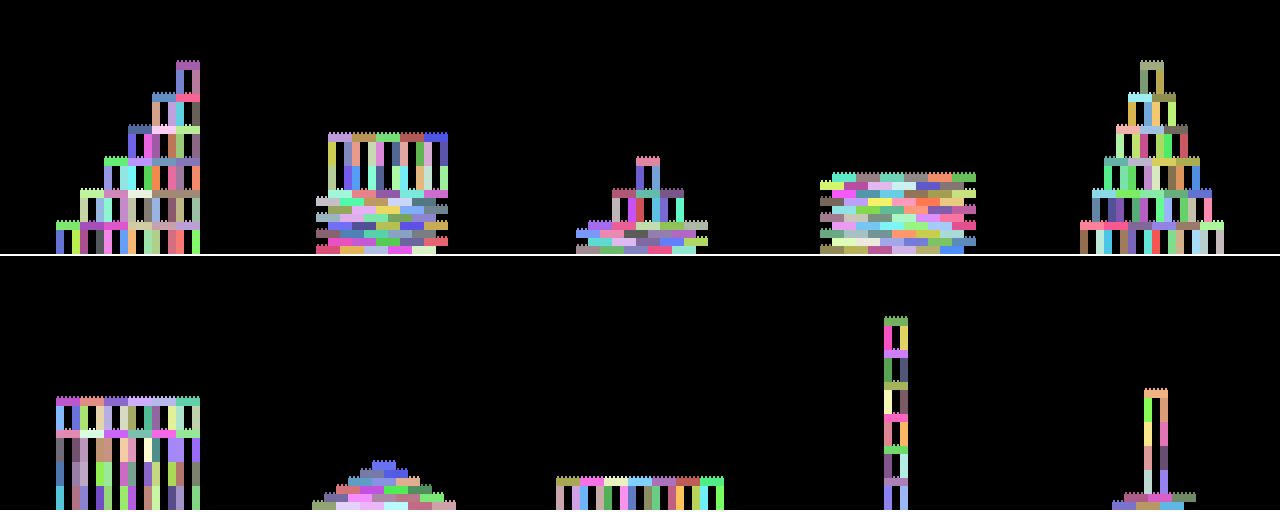
\includegraphics[width = \textwidth]{figures/tower_montage_10.png}}\\\midrule \\
    \toprule Example learned Library components&Samples written using final library\\\midrule
    \begin{tabular}{rl}
      Brickwall&\begin{tabular}{l}
        \includegraphics[width = 6cm]{figures/tower/tower_dsl_bricks.png}
      \end{tabular}\\
      Bridge&\begin{tabular}{l}
        \includegraphics[width = 6cm]{figures/tower/tower_dsl_bridge.png}
      \end{tabular}\\
      Staircase&\begin{tabular}{l}
        \includegraphics[width = 6cm]{figures/tower/tower_dsl_staircase.png}
        \end{tabular}
    \end{tabular}&
    \begin{tabular}{l}
      \includegraphics[width = 6cm]{figures/tower/dreams.png}
      \end{tabular}
    \\\bottomrule 
    \end{tabular}
  \caption{\textbf{Top}: Ten (out of 112) tower building tasks. Agent writes a program controlling a `hand' that builds the target tower. \textbf{Bottom left}: Three learned library routines. These components act like parametric options~\cite{stolle2002learning},
    giving higher-level building blocks that the agent can use to plan. \textbf{Bottom Right}: 16 random samples, or `dreams', built from learned library.}\label{tower}
\end{figure}




\subsubsection{Probabilistic Generative Modeling of Text}
Few-shot learning of simple generative concepts comes naturally to
humans, from learning new rules in natural language~\cite{marcus1999rule},
to learning routines for symbols and signs
\cite{lake2015human},
to learning new motor routines for producing words.
We investigate few-shot generative modeling by tasking our
agent with inferring a probabilistic regular expression from a small
number of strings, where these strings are drawn from CSV columns crawled from the web~\cite{mws}. Across wake/sleep cycles, our agent learns to learn
regular expressions that describe the structure of a typically occurring text concepts,
like numbers or dates.
Figure~\ref{qualitativeRegex} shows example model outputs on held out generative modeling tasks,
contrasting the full model with ablations that lesion either the library learning or recognition model training.
\begin{figure}
  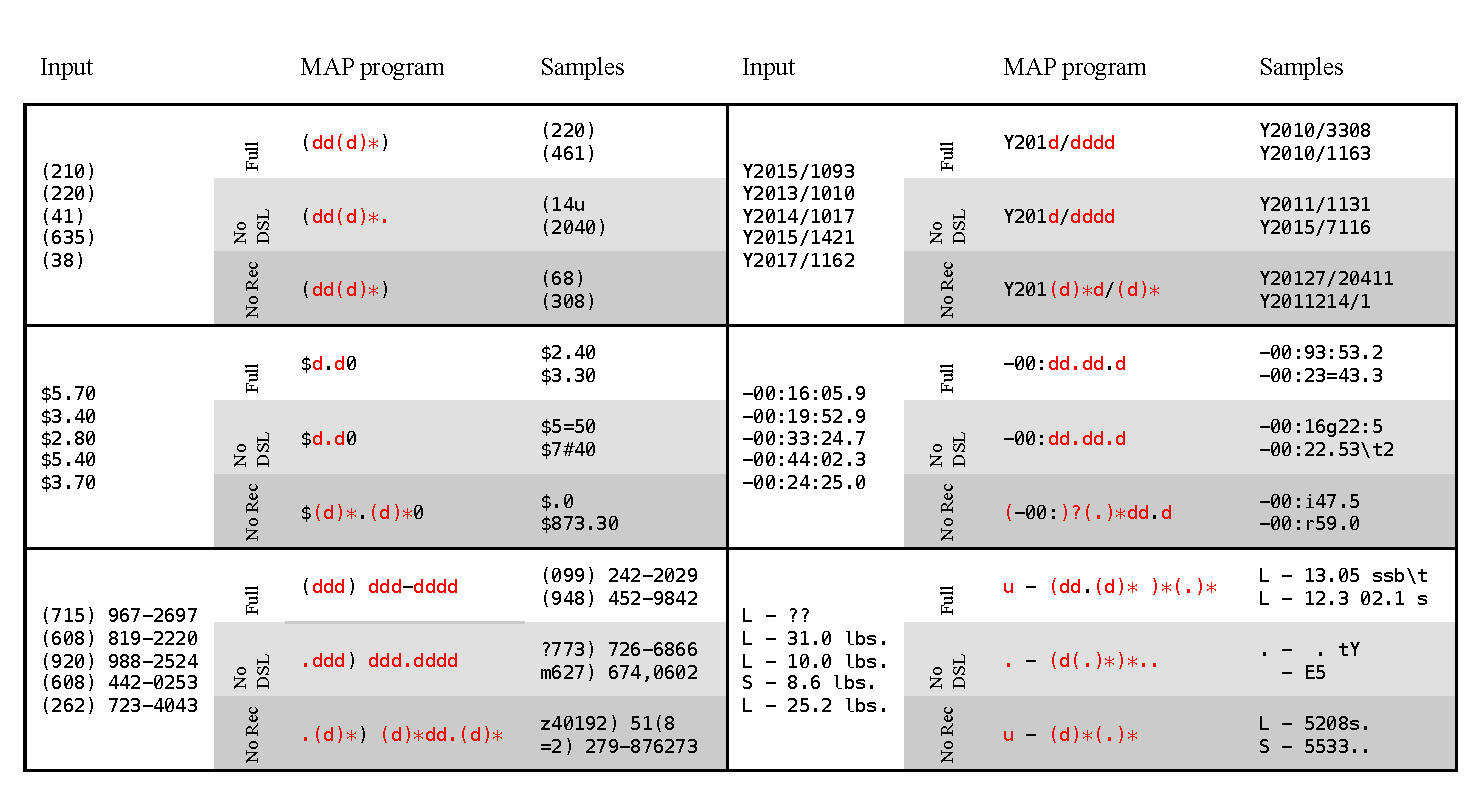
\includegraphics[width = \textwidth]{figures/regexQualitative.pdf}
  \caption{Qualitative results on probabilistic generative text modeling. Agent observes 5 strings (`Input' column) and infers a probabilistic regex (MAP program--regex primitives highlighted in red), from which it can imagine more examples of the latent text concept. No Library: Dreaming only (ablates library learning). No Rec: Consolidation only (ablates recognition model)}\label{qualitativeRegex}
\end{figure}

\subsection{From libraries to languages}

Rather than start with a domain-specific basis and then enrich it over successive wake/sleep cycles -- as these prior experiments have done --
could we instead start with a highly generic basis,
and then learn a library encoding something closer to the basic domain language?
We first consider learning a basic language for physical laws,
starting with generic sequence-manipulation primitives,
and then investigate how these fundamental sequence-manipulating routines could themselves be learned.

We first task \system with inferring 60 equations describing physical laws,
like closed forms for ballistic motion, inverse square laws,
expressions for calculating centers of mass, etc.,
which we took from AP and MCAT physics `cheat sheets'
along with equation guides from machine learning textbooks.
These relationships are easy to express
given concepts like vectors or forces.
Rather than `bake in' abstractions like these we
initialize the system with Lisp-style sequence manipulation primitives like
\code{map} and \code{fold}.
We automatically convert each task into a
regression problem by randomly generating real or vector valued input/outputs,
and encode vectors as lists of reals.

In solving these tasks, \system first discovers the building blocks of vector algebra,
like inner products, vector sums, and norms.
It then uses this vocabulary to infer library routines for common
physical relationships like the vector form inverse square laws
and integrating second derivatives over time,
effectively undergoing a `change of basis' from the initial Lisp-style primitives into a
physics-style basis. Figure~\ref{librariesToLanguages}~(left) illustrates a subset
of the provided tasks and learned library for this domain. 

\begin{figure}
  \centering
  \setlength{\tabcolsep}{2pt} % default is 6pt
  \begin{tabular}{lll}\toprule
    &\multicolumn{1}{c}{Physical Laws}&\multicolumn{1}{c}{Recursive Functions}\\\midrule
    \normalsize \rotatebox[origin=c]{90}{\pop{Programs} \& Tasks}&
    % physical laws programs and tasks
    \begin{tabular}{l}
      \begin{tabular}{l}
        Kinetic energy:\\
        $m$, $\vec{v}\mapsto \frac{1}{2}m|\vec{v}|^2$\\
        \code{1, [0 2 -1]$\to$2.5}\\
        \code{2, [2 1 3]$\to$14}\\
        %#(lambda (lambda (*. (/. $0 (+. $1 $1))))) 1. $1 (#(lambda (fold $0 0. (lambda (lambda (+. $0 (*. $1 $1)))))) $0))))
        \blueCode{$f(m$, $\vec{v}) = $($f_5$ 1 $m$ ($f_0$ $\vec{v}$))}
        
        %% Center-of-mass:\\
        %% $m_1$, $\vec{r}_1$, $m_2$, $\vec{r}_2\mapsto \frac{m_1}{m_1 + m_2}\vec{r}_1 + \frac{m_2}{m_1 + m_2}\vec{r}_2$\\
        %% \code{2, [3 0 1], 4, [0 6 0]}$\to$\code{[1 4 0.333]}\\
        %% \code{5, [7 1 6], 5, [9 2 2]}$\to$\code{[8 0.5 4]}        
      \end{tabular}\\\\
      \begin{tabular}{l}
        Coulomb's law:\\
        $q_1$, $\vec{r}_1$, $q_2$, $\vec{r}_2\mapsto \frac{q_1q_2}{|\vec{r}_1 - \vec{r}_2|_2^2} \times \frac{\vec{r}_1 - \vec{r}_2}{|\vec{r}_1 - \vec{r}_2|}$\\
        \code{4, [1 5 2], 2, [2 5 2]$\to$[-8 0 0]}\\
        \code{-1, [0 1 1], -1, [0 0 0]$\to$[0 0.5 0.5]}        \\
        \blueCode{$f(q_1$, $\vec{r}_1$, $q_2$, $\vec{r}_2) = $}\\
        \hspace{0.2cm}\blueCode{($f_{10}$ $q_1$ $q_2$ (zip $\vec{r}_1$ $\vec{r}_2$ ($\lambda$ (x y) (- x y))))}
      \end{tabular}\\\\
      \begin{tabular}{l}
        %% Integrating angle over time:\\
        %% $\theta_0$, $\omega_0$, $\alpha$, $t\mapsto \frac{1}{2}\alpha t^2 + \omega_0t + \theta_0$\\
        %% \code{1, 3, 0, 2$\to$7}\\
        %% \code{-5, 0, 10, 1$\to$0}\\
        %% \blueCode{$f(\theta_0$, $\omega_0$, $\alpha$, t$) = $($f_5$ $\omega_0$ $\theta_0$ $\alpha$ t)}
        Newton's Second Law:\\
        $m$, $\{\vec{F}_i \}\mapsto \frac{1}{m}\sum_i\vec{F}_i = a$\\
        \code{2, [[2 4 1]]$\to$[1 2 0.5]}\\
        \code{3, [[0 0 2] [3 0 1]]$\to$[1 0 0.333]}\\
        \blueCode{$f(m$, forces$) = $($f_4$ ($f_7$ m) ($f_3$ forces))}
        \end{tabular}
      \end{tabular}
    &
    % recursive functions programs and tasks
    \begin{tabular}{l}
      \begin{tabular}{l}
        Duplicate each list element:\\
        \code{[9 2]$\to $[9 9 2 2]}\\
        \code{[5 0 3]$\to $[5 5 0 0 3 3]}\\
        \code{[1 2 3 4]$\to $[1 1 2 2 3 3 4 4]}\\
        \blueCode{$f(l) = $($f_0$ ($\lambda$ (x a) (cons x (cons x a))) l nil)}        
      \end{tabular}\\\\

      \begin{tabular}{l}
        Lengths of list-of-lists:\\
        \code{[[2 1] [1 2 9]\, []]}$\to $\code{[2 3 0]}\\
        \code{[[5 2 9 3 7 5 2]]}$\to $\code{[7]}\\
        \code{[[] [] [9 8 9 9]]$\to$[0 0 4]}\\
        \blueCode{$f(\ell) = $($f_2$ ($\lambda$ (z) ($f_4$ z)) $\ell$)}
      \end{tabular}\\\\
      \begin{tabular}{l}
        1-index into list:\\
        \code{1, [9 2 3]$\to $9}\\
        \code{2, [1 5 8]$\to $5}\\
        \code{4, [0 2 8 1 5 6]$\to $1}\\
        \blueCode{$f($n$,$l$) = $($f_8$ l (+ 1 n))}
      \end{tabular}\\\\
      
      
      \end{tabular}
    \\\midrule
    \rotatebox[origin=c]{90}{\popp{Library}}&
    % physical laws library
    \begin{tabular}{l}
      \begin{tabular}{l}
        \greenCode{$f_0($v$)\,=\,$(fold 0 ($\lambda$ (x y) (+ (* x x) y)) v)}\\
        \hspace{\helpSize}($f_0$: \emph{L-2 norm}) % still here
      \end{tabular}\\
      \begin{tabular}{l}
        \greenCode{$f_1($v$)\,=\,$(fold 0 ($\lambda$ (x y) (+ x y)) v)}\\
        \hspace{\helpSize}($f_1$: \emph{Sum vector components}) % still here
      \end{tabular}\\
      \begin{tabular}{l}
        \greenCode{$f_2($v,u$)\,=\,$($f_1$ (zip v u ($\lambda$ (x y) (* x y))))}\\
        \hspace{\helpSize}($f_2$: \emph{Dot product}) % still here
      \end{tabular}\\ 
      \begin{tabular}{l}
        \greenCode{$f_3($vs$)\,=\,$(fold vs (map ($\lambda$ (x) (* x 0))}\\
        \phantom{\greenCode{$f_3($vs$)\,=\,$(fold vs (}}\greenCode{(car vs))}\\
        \phantom{\greenCode{$f_3($vs$)\,=\,$(}}\greenCode{($\lambda$ (v u) (zip v u ($\lambda$ (x y) (+ x y)))))}\\
        \hspace{\helpSize}($f_3$: \emph{Sum (list of) vectors}) % still here
      \end{tabular}\\
      \begin{tabular}{l}
        \greenCode{$f_4($x,v$)\,=\,$(map ($\lambda$ (y) (* x y)) v)}\\
        \hspace{\helpSize}($f_4$: \emph{Multiply vector by scalar})
        \end{tabular}\\
      \begin{tabular}{l}
        \greenCode{$f_5($x,y,z$)\,=\,$(* (/ y (+ x x)) z)}
      \end{tabular}\\
      \begin{tabular}{l}
        \greenCode{$f_6($x,y$)\,=\,$(* ($f_5$ 1 x y) x)}\hspace{1cm}\greenCode{$f_7($x$)\,=\,$(/ 1 x)}
      \end{tabular}\\
      %      %#(lambda (lambda (lambda (lambda (+. $2 (*. $0 (+. (*. (#(lambda (/. $0 (+. 1. 1.))) $0) $1) $3))))))) $2 $3 $1 $0)))))
      %% \begin{tabular}{l}
      %%   \greenCode{$f_5($v,x,a,t$)\,=\,$(+ x (* t (+ (* ($f_4$ t) a) v)))}\\
      %%   \hspace{\helpSize}($f_5$: \emph{Integrate given first and second derivatives})
      %% \end{tabular}\\
      \begin{tabular}{l}
        \greenCode{$f_8($v$)\,=\,$(power ($f_0$ v) ($f_6$ 1 1))}\\
        \hspace{\helpSize}($f_8$: \emph{vector length})
      \end{tabular}\\
      %(lambda (lambda (lambda (map (lambda (*. (/. (*. (/. $0 (#(lambda (fold $0 0. (lambda (lambda (+. (*. $1 $1) $0))))) $1)) $3) (#(lambda (power (#(lambda (fold $0 0. (lambda (lambda (+. (*. $1 $1) $0))))) $0) (#(lambda (/. $0 (+. 1. 1.))) 1.))) $1)) $2)) $0)
      %(lambda (lambda (lambda (map ($\lambda$ (x) (* (/ (* (/ x ($f_0$ v)) a) ($f_6$ v)) b)) v)
      \begin{tabular}{l}
        \greenCode{$f_9($x,y,z$)\,=\,$(* (/ x ($f_0$ z)) y)}\\
        \hspace{\helpSize}($f_9$: \emph{scalar form of inverse square law})
      \end{tabular}\\
      \begin{tabular}{l}
        \greenCode{$f_{10}($x,y,v$)\,=\,$($f_4$ ($f_9$ y (/ x ($f_7$ v)) v) v)}\\
        \hspace{\helpSize}($f_{10}$: \emph{vector form of inverse square law})
        \end{tabular}
    \end{tabular}
    
    &
    % recursive functions programs and tasks
    \begin{tabular}{l}
      \begin{tabular}{l}
        \popp{\code{$f_0($f$,$l$,$x$)\,=\,$(if (empty? l) x}}\\
        \phantom{\code{$f_0($f$,$l$,$x$)\,=\,$(if }}}\popp{\code{(f (car l) ($f_0$ (cdr l))))}}\\
          \hspace{\helpSize}($f_0$: \emph{fold})
      \end{tabular}\\
      \begin{tabular}{l}
        \popp{\code{$f_1($p$,$f$,$n$,$x$)\,=\,$(if (p x) nil}}\\
        \phantom{\code{$f_1($f$,$l$,$x$)\,=\,$(if }}}\popp{\code{(cons (f x) ($f_1$ (n x))))}}\\
          \hspace{\helpSize}($f_1$: \emph{unfold})
      \end{tabular}\\
      \begin{tabular}{l}
        \greenCode{$f_2($f$,$l$)\,=\,$($f_0$ nil l ($\lambda$ (x a) (cons (f x) a)))}\\
        \hspace{\helpSize}($f_2$: \emph{map})
      \end{tabular}\\
      \begin{tabular}{l}
        \greenCode{$f_3($f$,$p$,$n$)\,=\,$($f_1$ p f (+ 1) n)}\\
        \hspace{\helpSize}($f_3$: \emph{count upward until predicate holds})
      \end{tabular}\\
      \begin{tabular}{l}
        \greenCode{$f_4($l$)\,=\,$($f_0$ ($\lambda$ (a x) (+ 1 a)) l 0)}\\
        \hspace{\helpSize}($f_4$: \emph{length})
      \end{tabular}\\
      \begin{tabular}{l}
        \greenCode{$f_5($p$)\,=\,$($f_3$ ($\lambda$ (x) x) p 0)}\\
        \hspace{\helpSize}($f_5$: \emph{count upward from 0 until predicate holds})
      \end{tabular}\\
      \begin{tabular}{l}
        \greenCode{$f_6($n$)\,=\,$($f_5$ (eq? n))}\\
        \hspace{\helpSize}($f_6$: \emph{range})
      \end{tabular}\\
      \begin{tabular}{l}
        \greenCode{$f_7($f$,$l$)\,=\,$($f_0$ nil l ($\lambda$ (x a) (if (f x) a (cons x a))))}\\
          \hspace{\helpSize}($f_7$: \emph{filter})
      \end{tabular}\\
      \begin{tabular}{l}
        \greenCode{$f_8($l$,$n$)\,=\,$(car ($f_0$ ($\lambda$ (a x) (cdr a)) ($f_6$ n) l))}\\
        \hspace{\helpSize}($f_8$: \emph{index})
      \end{tabular}
      
      
      
      
    \end{tabular}

    \\\bottomrule 
    
  \end{tabular}
  \setlength{\tabcolsep}{6pt} % default is 6pt
  \caption{\textbf{Left:} Learning a language for physical laws starting with recursive list routines like \code{map} and \code{fold}. Agent observes input/outputs of latent functions encoding physical laws (top left, 20 input/outputs per task). Vectors are represented as lists of real numbers. Physical constants expressed in Planck units. \textbf{Right:} Learning a language for recursive list routines starting with only recursion and primitives found in 1959 Lisp. Agent rediscovers \code{map}, \code{fold}, \code{unfold}, etc. For full tasks and learned libraries see Appendix~\ref{appendixMcCarthy}}\label{librariesToLanguages}
  \end{figure}

Could we also learn the basics of programming, including these recursive sequence manipulation primitives?
This goal is relevant to a long-standing dream within the program induction community to ``learn from scratch'': starting with a \emph{minimal} Turing-complete programming language,
and then learning to solve a wide swath of
induction problems~\cite{solomonoff1964formal,schmidhuber2004optimal,hutter2004universal,solomonoff1989system}.
All existing systems,
including ours,
fall far short of this dream,
and it is unclear (and we believe unlikely)
that this dream could ever be fully realized.
How far can we push in this direction?
``Learning from scratch'' is subjective, but a reasonable
starting point is the set of primitives provided in 1959
Lisp~\cite{mccarthy1960recursive}: these include
conditionals, recursion, arithmetic, and the 
list operators \code{cons}, \code{car}, \code{cdr}, and \code{nil}.
A  basic first goal is to start with
these primitives,
and then recover a representation that
more closely resembles modern functional languages like Haskell and OCaml.

We ran the following experiment: \system was given a subset of the
1959 Lisp primitives, and tasked with solving 18 programming
exercises. A key difference between this setup and our previous
experiments is that, for this experiment, the system is given
primitive recursion, whereas previously we had sequestered recursion
within higher-order functions like \code{map}, \code{fold}, and
\code{unfold}.  In solving these 18 exercises, the algorithm assembles
a library containing a modern repertoire of functional programming idioms
and subroutines, including \code{map}, \code{fold}, \code{unfold},
\code{index}, \code{length}, and arithmetic operations like building
lists of natural numbers between an interval (see
Figure~\ref{librariesToLanguages}, right).

We believe that program learners should \emph{not}
start from scratch,
but instead should start from
a rich, domain-agnostic
basis like those embodied in the standard libraries of modern  languages.
What these experiments reveal is that \system doesn't \emph{need} to start from a rich basis,
and can in principle recover many of the amenities of modern programming systems,
provided it is given enough computational power and a suitable
spectrum of tasks.



\subsection{Analyzing \system across domains}\label{quantitative}
To evaluate the relative importance of library learning and recognition
model training, we evaluate on held-out testing tasks for each of our
domains, measuring both how many tasks are solved and how long it
takes to solve them across successive wake/sleep iterations
(Fig.~\ref{learningCurves}).  We always solve more held-out tasks --
and generally solve them in less time -- with both components
combined, suggesting a synergy between these forms of declarative and procedural knowledge.
Examining the libraries learned with and without
recognition models reveals a difference in the typical \emph{depth}
of learned subroutines, and this average depth correlates
with the number of solved testing tasks ($r=0.71$, $p < 10^{-8}$).
In contrast, the correlation between the \emph{number} of learned subroutines and number of solved tasks is weaker and not statistically significant ($r=0.20$, $p > 0.05$),
suggesting that the recognition model bootstraps
``better'' libraries, where ``better'' is at least partly explained by the depth
of the learned representation. Figure~\ref{depthMontage} shows typical `deep' libraries learned by
\system and contrasts this depth with \% solved tasks, both with and without the recognition model.
\begin{figure}
  \begin{tabular}{ccc}
    \begin{tabular}{c}
      \includegraphics[width = 5cm]{figures/learningCurves/text_hits.png}\\
      \includegraphics[width = 5cm]{figures/learningCurves/text_time.png}
    \end{tabular}&

    \begin{tabular}{c}
      \includegraphics[width = 5cm]{figures/learningCurves/logo_hits.png}\\
      \includegraphics[width = 5cm]{figures/learningCurves/logo_time.png}
    \end{tabular}&
    
    \begin{tabular}{c}
      \includegraphics[width = 5cm]{figures/learningCurves/rational_hits.png}\\
      \includegraphics[width = 5cm]{figures/learningCurves/rational_time.png}
    \end{tabular}\\\\\\

    \begin{tabular}{c}
      \includegraphics[width = 5cm]{figures/learningCurves/list_hard_hits.png}\\
      \includegraphics[width = 5cm]{figures/learningCurves/list_hard_time.png}
    \end{tabular}&

    \begin{tabular}{c}
      \includegraphics[width = 5cm]{figures/learningCurves/tower_hits.png}\\
      \includegraphics[width = 5cm]{figures/learningCurves/tower_time.png}
    \end{tabular}&

    \begin{tabular}{c}
      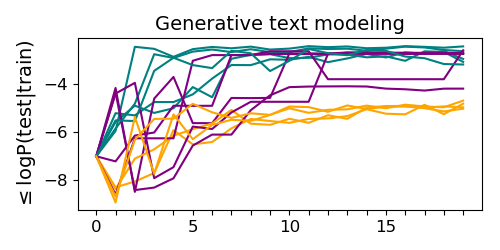
\includegraphics[width = 5cm]{figures/learningCurves/regex_marginal_test_unigram_gen.png}\\
      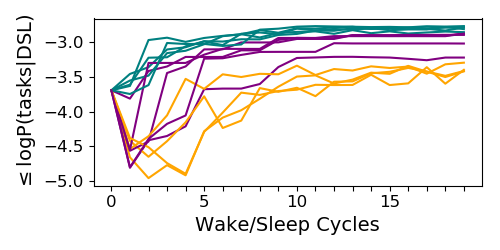
\includegraphics[width = 5cm]{figures/learningCurves/regex_task_train_unigram_gen.png}
      \end{tabular}
  \end{tabular}
  \caption{Test set performance across wake/sleep iterations. Each curve is a run with a different random seed. Teal: Full model. Orange: Dreaming only (no library learning). Purple: Consolidation only (no recognition model). Search time plots show solid lines (time averaged over all tasks) and dotted lines (time averaged over solved tasks). Generative text modeling plots show (top) posterior predictive likelihood of held-out strings on held out tasks and (bottom) lower bound on marginal likelihood of held out tasks, both of which are averaged per character.}\label{learningCurves}      
\end{figure}

\begin{figure}
  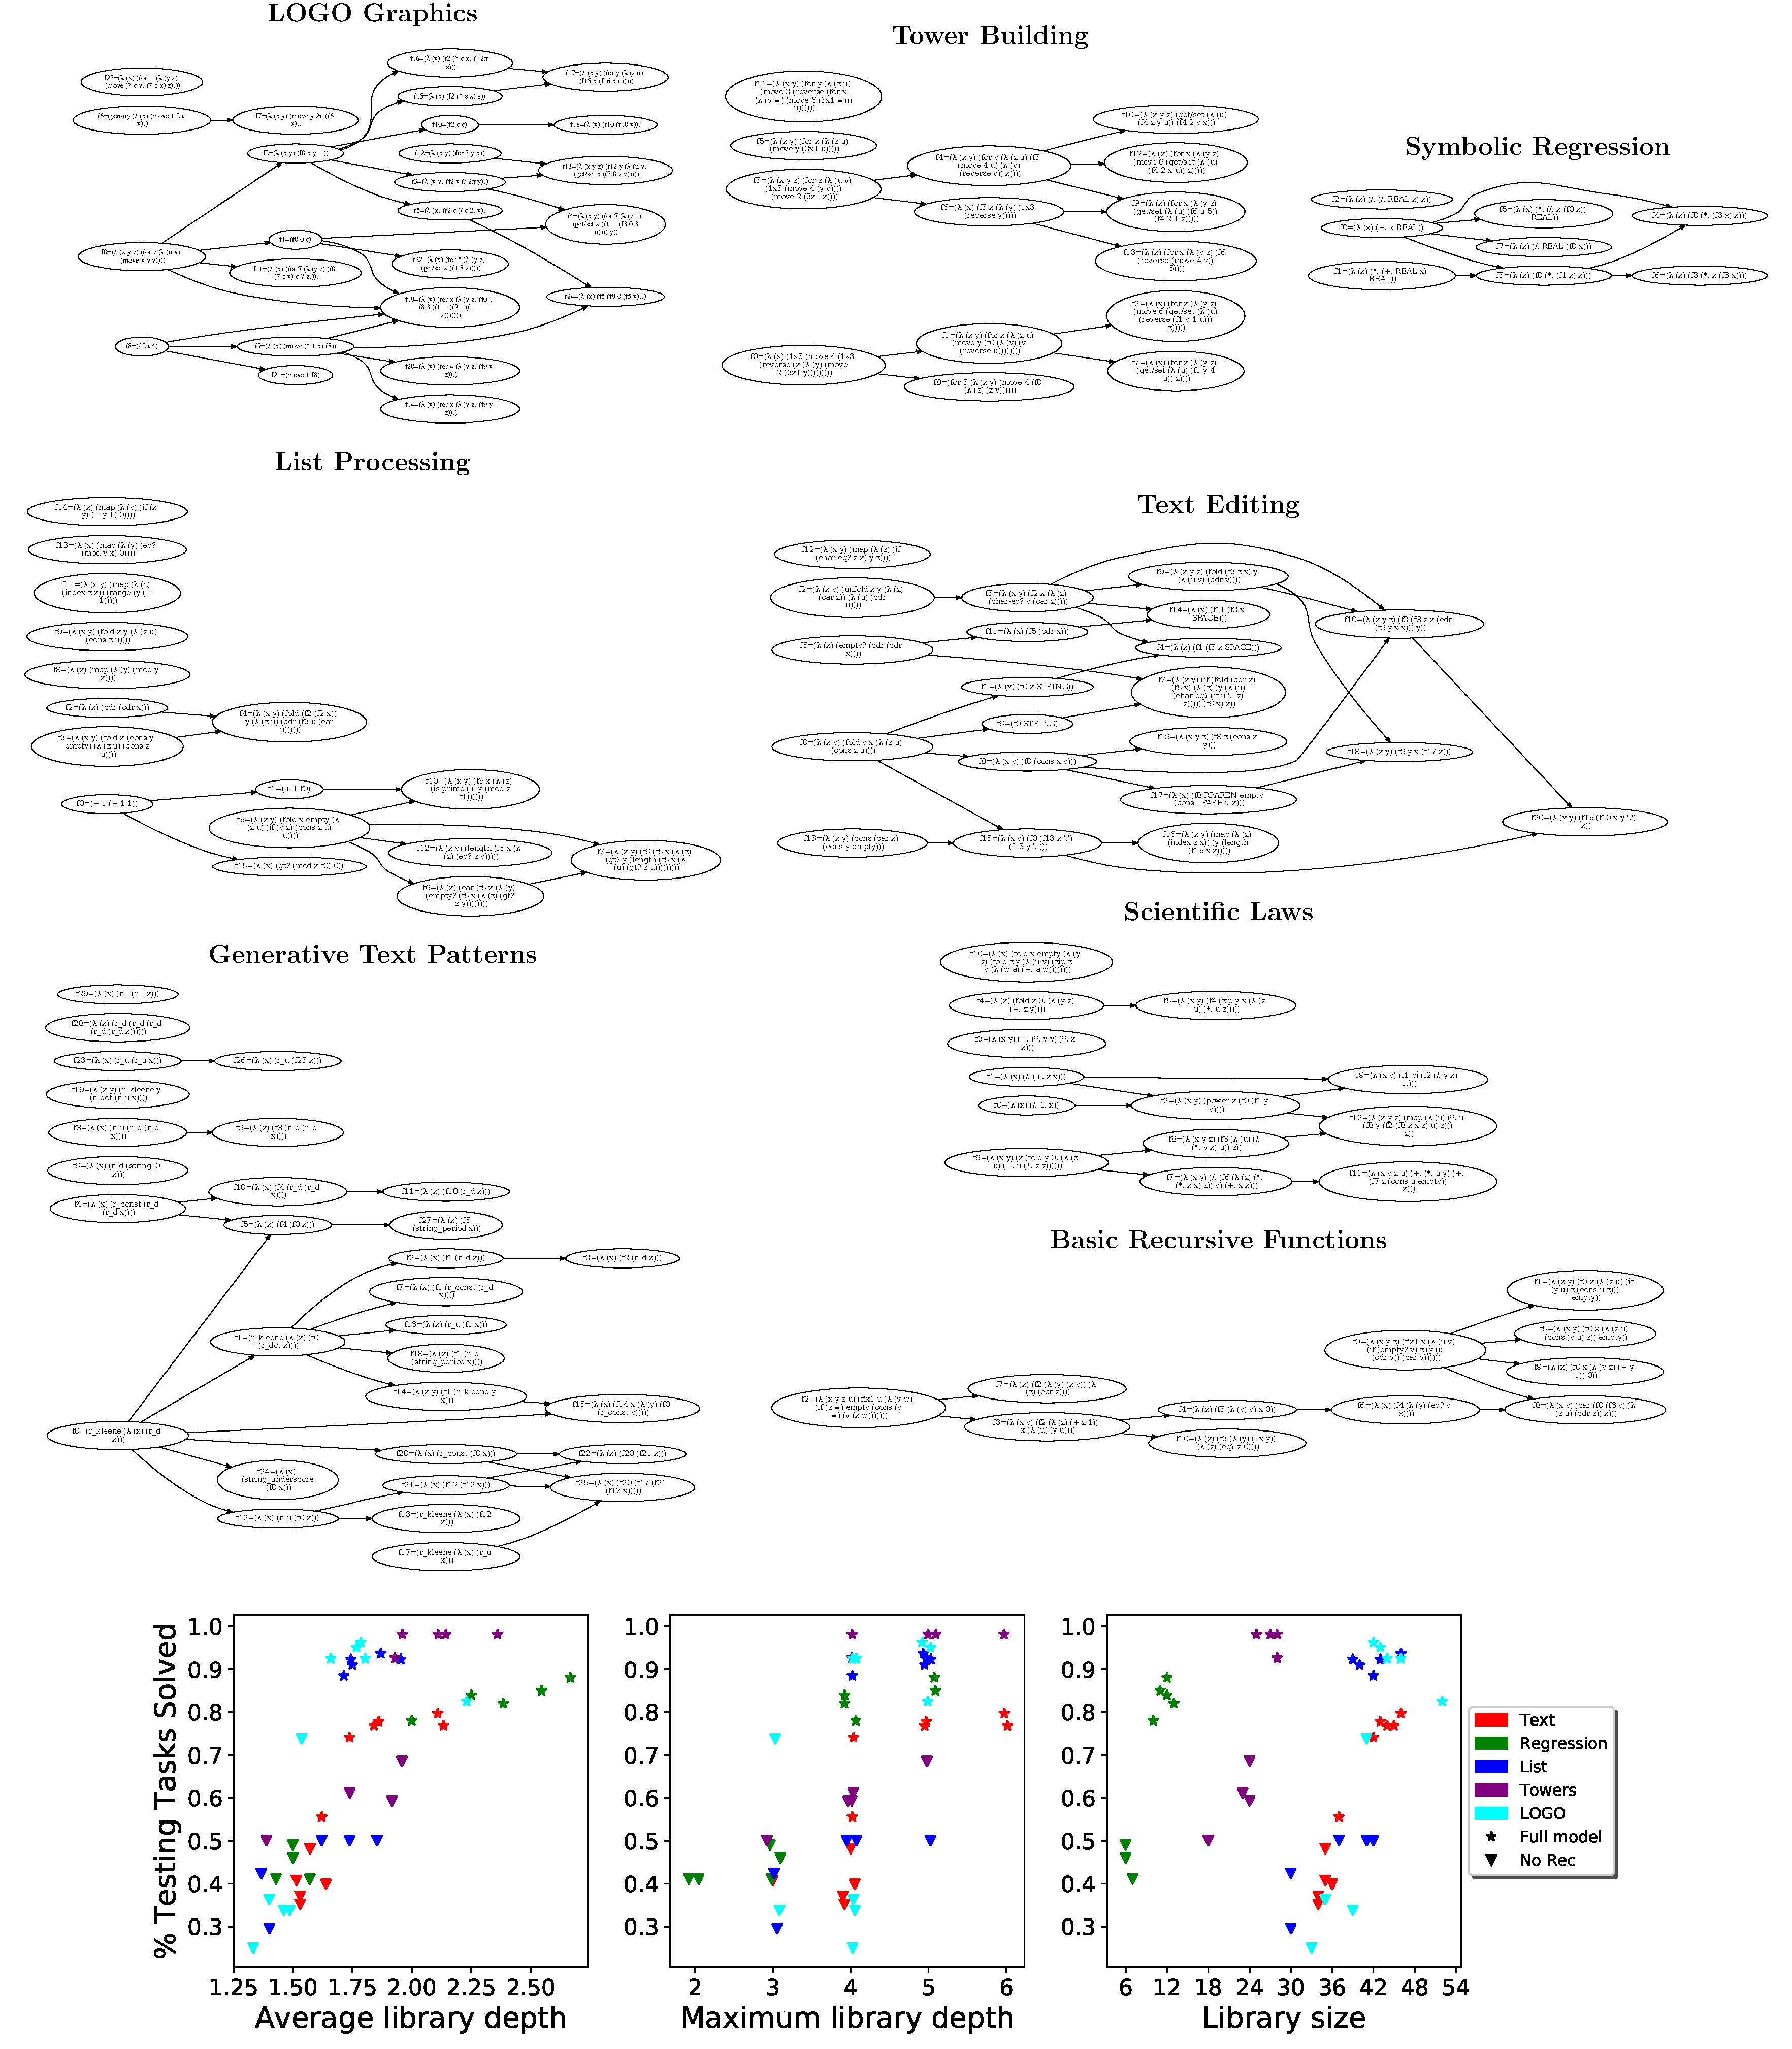
\includegraphics[width = \textwidth]{deepMontage.pdf}
  \caption{Top: Learned libraries diagrammed as networks. Arrows point from a learned concept to all other concepts that use it. Bottom: Deeper networks solve more testing tasks, both as measured by average depth (left) and maximum depth (middle), while total library size is more weakly associated with solving tasks (right). Full model (stars on scatterplots) learns deeper libraries than no-recognition-model ablation (triangles on scatterplots). Each scatter plot point run with a different random seed.}\label{depthMontage}
\end{figure}

How do \systemEnding's representations of these tasks themselves change, as the model acquires expertise? Within cognitive science, a rich body of evidence suggests that human experts learn to `see' problems differently in their domains -- even before solving a problem, human novices and experts seem to construct fundamentally different initial representations \cite{chi1981categorization}. Novices notice a problem’s `surface features', the literal objects and details made obvious by the task description. Experts, on the other hand, somehow see past these details to pick out each problem’s `deep structures', the underlying principles and concepts that govern its ultimate solution \cite{chi2012seeing,chi2006two}.


\systemEnding's neural recognition model can be seen as forming analogous `initial' problem representations, implicitly encoded within the activations of the neural network. Intuitively, these initial neural representations map problem features to a `gist' over the model’s current domain-specific concepts -- they guide and constrain how the model searches for problem solutions, but are not symbolically structured solutions themselves. To probe how these representations change as the model gains a richer conceptual vocabulary within each domain, we compare how they cluster problems within that domain over the course of \systemEnding's learning trajectory. Figure \ref{textExpertiseCluster} depicts TSNE visualizations of these neural problem representations at the first and last iteration of the algorithm. We color-code each problem using semantic, human-interpretable categories determined apriori by the task designers, but critically, the model itself never has access to these categories. Rather, as \system acquires domain expertise, the neural network adapts how it transforms each task's surface features, restructuring its initial problem representation space to draw together problems that share deeper, more abstract conceptual similarities.

\begin{figure}
  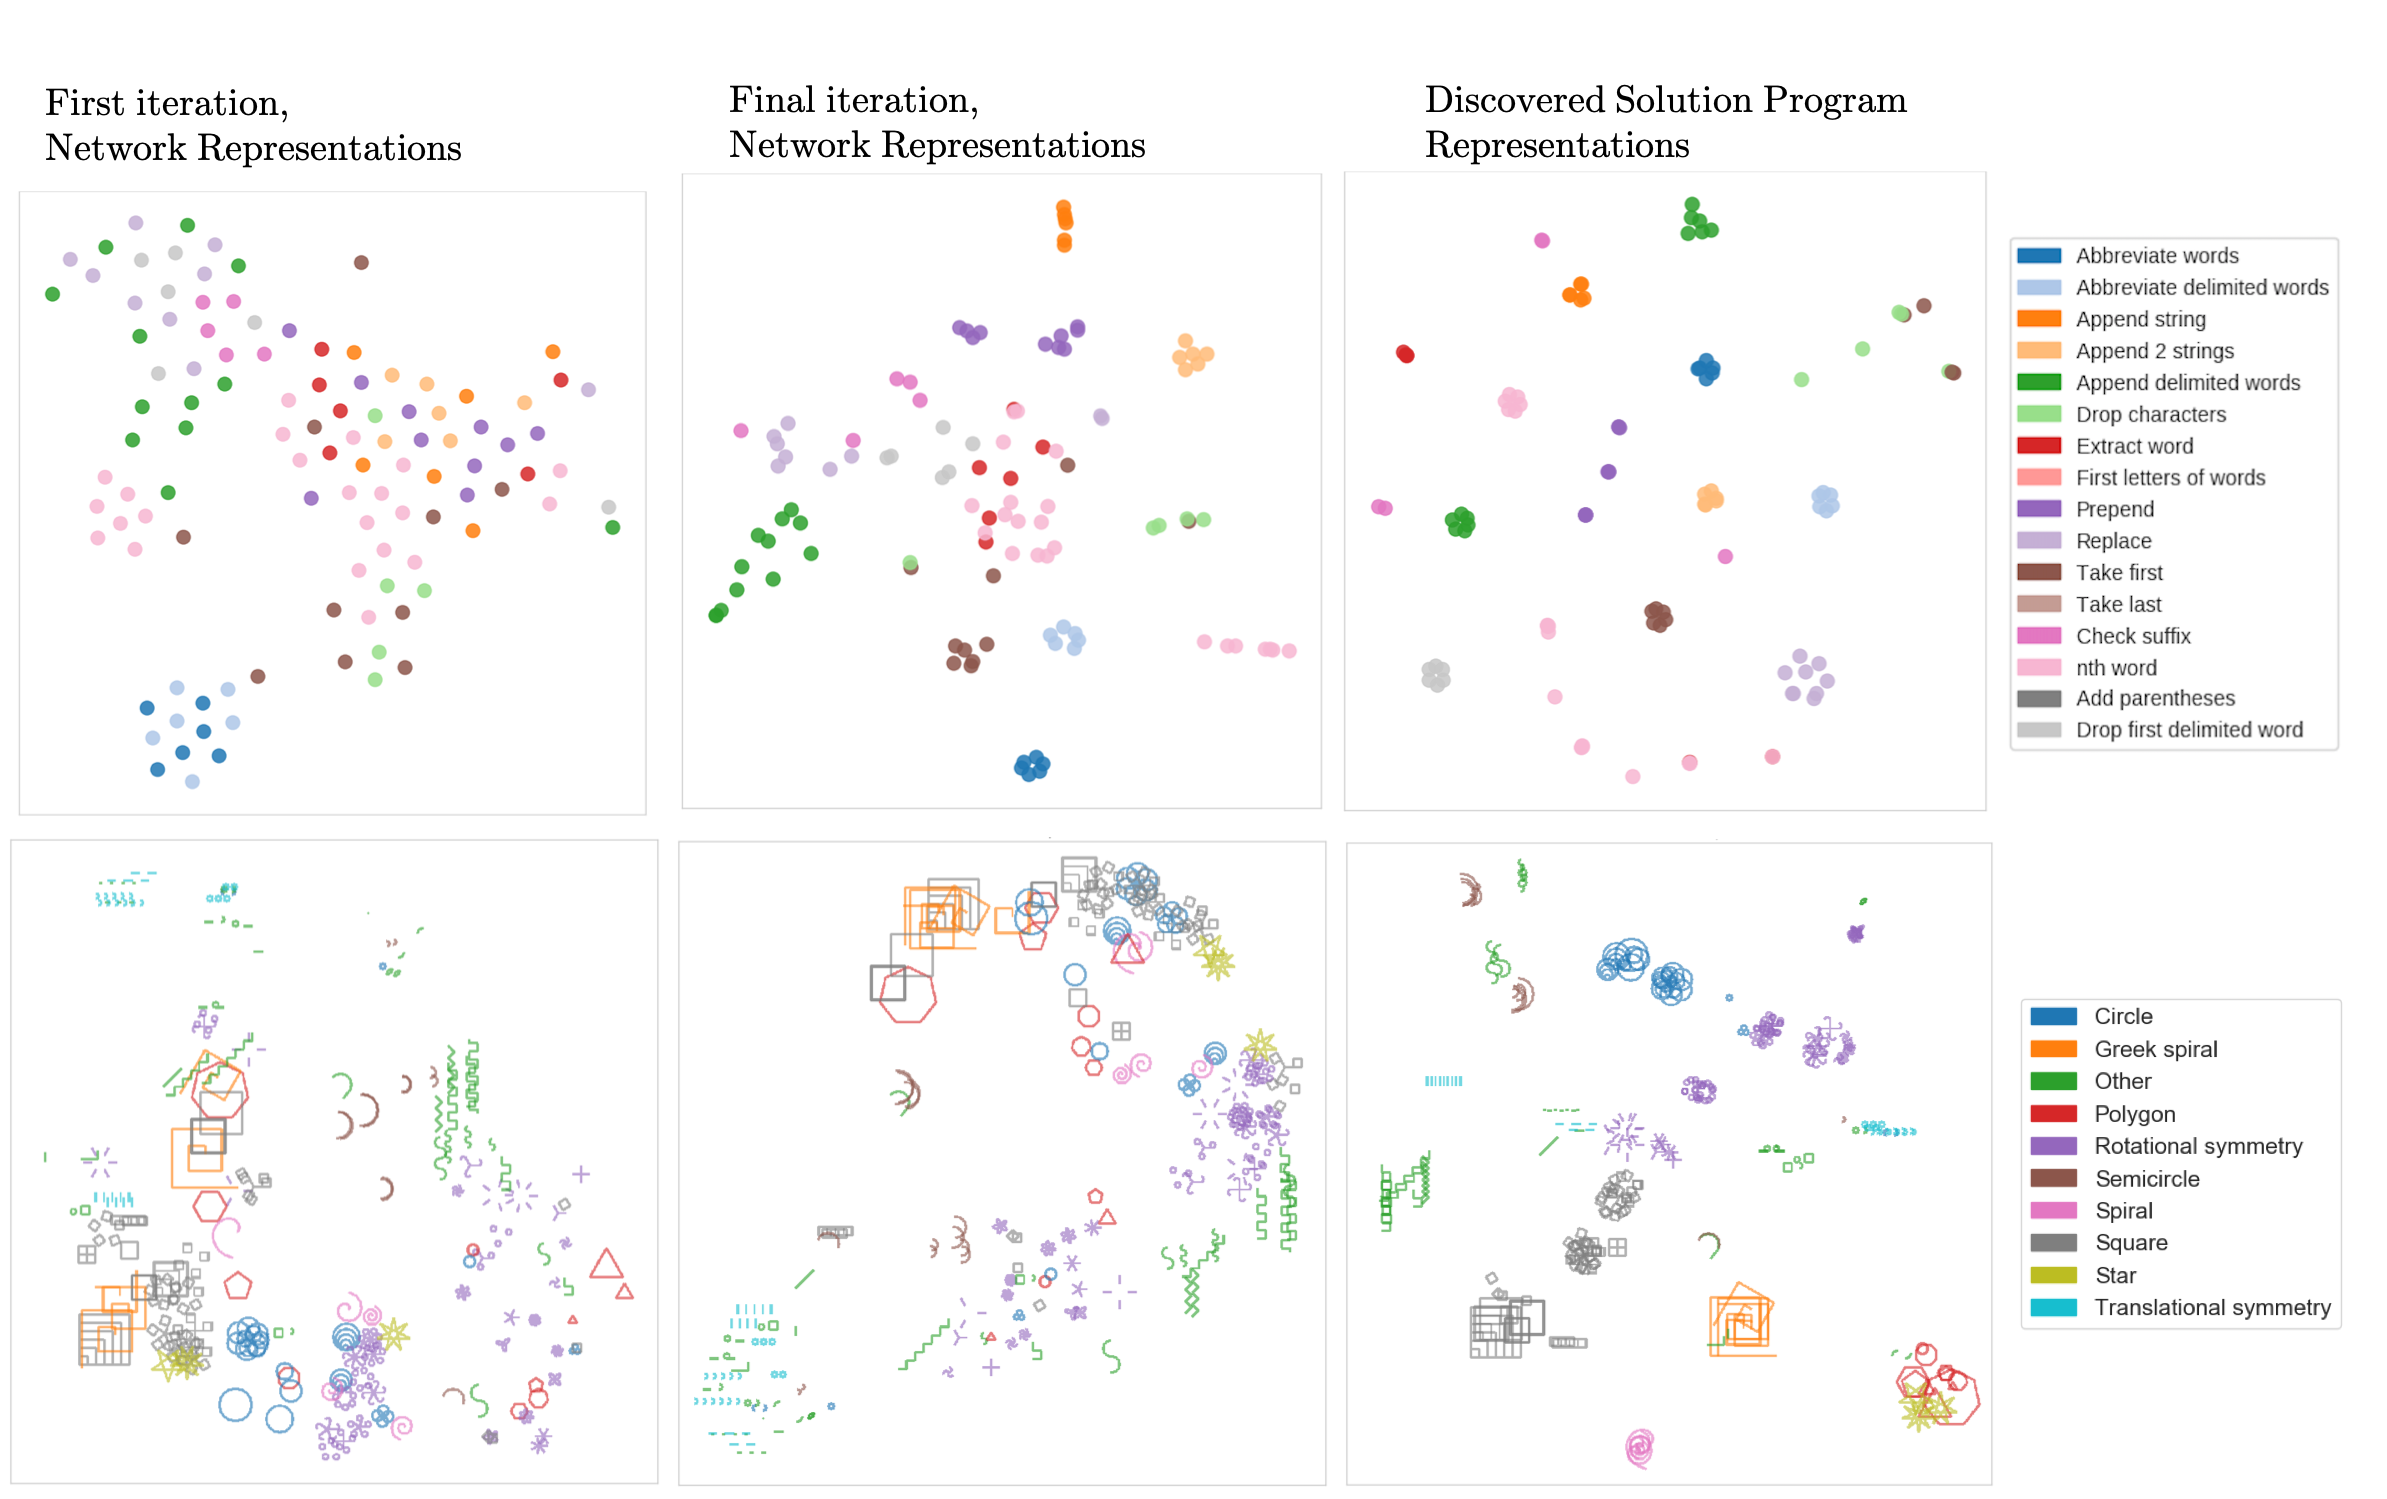
\includegraphics[width = \textwidth]{figures/textLogo_tsne.png}
  \caption{Left: TSNE embedding of model's `at-a-glance' (before searching for solution) organization of tasks (neural net activations), after first wake/sleep cycle. Middle: at-a-glance organization after last wake/sleep cycle. Right: TSNE visualization of programs actually used to solve tasks; intuitively, how model organizes tasks after searching for a solution. We convert each program into a feature vector by counting the \# times each library routine is used, and then embed those feature vectors. More examples in Fig.~\ref{allTSNE}}\label{textExpertiseCluster}
\end{figure}



\section{Discussion}

Our goal was to build a model capturing
humanlike aspects of learning to be an expert in a new domain of
problems. Our model works through a wake/sleep algorithm that grows an increasingly deep
representation of a domain's conceptual structure,
while learning to quickly combine these concepts into programs
solving specific problems within the domain.
Two main findings of our work are that, first, a single
program-induction system can learn to solve large sets of problems
from many qualitatively different domains; and second, that fully
acquiring expertise in these domains hinges both upon explicit
declarative knowledge, and implicit procedural skill.  We have
deliberately placed the interplay of declarative and procedural
knowledge at the center of our model, and believe that both these
kinds of learning are crucial for building agents that, like humans,
autonomously learn to navigate a new domain of problems.

\system builds on several generations of research in AI, program synthesis,
and cognitive science, with program induction being one of the oldest
theoretical frameworks for concept learning within artificial
intelligence~\cite{solomonoff1964formal}, and the conceptually allied
`Language of Thought Hypothesis' being almost as
old~\cite{fodor1975language}. Recent neural program synthesis systems
pair a fixed domain-specific programming language (a `DSL') to a
learned neural network that guides program
search~\cite{DBLP:journals/corr/abs-1804-01118,balog2016deepcoder,devlin2017neural}, while recent
symbolic AI research has developed frameworks for learning the DSL by
inferring reusable pieces of
code~\cite{ecc,Dechter:2013:BLV:2540128.2540316,DBLP:conf/icml/LiangJK10,DBLP:conf/ecai/LinDETM14}.
A main goal of this work is to combine and refine these techniques
with the intention of building agents that, like humans, develop
domain expertise for new classes of problems.  Work in cognitive
modeling has often exploited program-like representations for both
concept~\cite{piantadosi2011learning,lake2015human,GoodmanEtAl2015-Chapter} and intuitive theory
learning~\cite{logical,Ullman2012},
and we view these models of concept learning as
a kind of program induction,
and see theory learning as similar to inducing a DSL or library.


Our model draws on ideas first elucidated by the
Exploration-Compression family of algorithms~\cite{Dechter:2013:BLV:2540128.2540316,ecc,lazaro2019beyond,DBLP:conf/icml/LiangJK10,solomonoff1989system,schmidhuber2004optimal,ozkural2011teraflop},
which alternate
between searching, or `exploring', a space of solutions, and then
updating their search procedure by compressing solutions found during
exploration.  Both of our sleep phases can be interpreted as a kind of
compression: abstraction aims to compactly refactor code, while the
recognition model aims to encode a program in as few bits as possible,
conditioned on a task. What \system contributes here is the joint capture of
declarative aspects of domain knowledge -- considered in prior EC works -- and
the equally crucial procedural knowledge,
both of which human experts seem to need.


%% Our model alternatingly searches for solutions to tasks and then improves its search strategy;
%% within program induction, these principles were first elucidated by the Exploration-Compression (EC) algorithm~\cite{Dechter:2013:BLV:2540128.2540316}.

%% Our work  sits within the Exploration-Compression (EC) family of
%% algorithms.%%  Our previous work, EC$^2$~\cite{ecc}, introduced
%% %% neurally-guided search into the EC framework and served as the
%% %% starting point for \systemEnding.  Our work here extends EC$^2$ by (1)
%% %% introducing a new refactoring compression algorithm, (2) enriching the
%% %% neural network with a new bigram-over-trees parameterization and loss
%% %% function that together learn to break symmetries, accelerating program
%% %% search during waking, and (3) demonstrating how this family of
%% %% approaches can be applied to planning and generative modeling
%% %% problems. 
%% Other offshoots of EC include our prior work, EC$^2$~\cite{ecc}, the neurosymbolic framework
%% in~\cite{lazaro2019beyond} and the hierarchical Bayesian program
%% learner in~\cite{DBLP:conf/icml/LiangJK10}. Closely aligned ideas go
%% even further back~\cite{solomonoff1989system,schmidhuber2004optimal}.




Our model's domain knowledge grows over a series of wake/sleep cycles,
with the solutions to easier problems bootstrapping
solving of harder tasks.
This dynamic is related to, but distinct from, curriculum learning. In curriculum learning approaches an agent solves a stream of pedagogically selected, increasingly difficult tasks; here we consider the case with the agent lacks a `teacher' and instead self-paces its way through an implicit curriculum.
But humans select their tasks in much richer ways,
and can even generate their own tasks to solve,
either as stepping stones toward hard, unsolved problems or motivated by considerations like curiosity and aesthetics.
Building agents that generate their own problems in these humanlike ways is a necessary next step
if we want machines that push against boundary of human domain knowledge or which even discover whole new domains of problems,
both of which go far beyond the relatively small-scale demonstrations in this work.

%% Over a lifetime humans develop expertise in many domains --
%% unlike our model,
%% which learned to solve many classes of problems,
%% but only class one at a time.
%% Scaling approaches like ours to this multidomain, lifelong setting
%% could be enabled by a hierarchical Bayesian model of DSLs for many domains,
%% capturing  shared conceptual structure between similar domains  (e.g., Parcheesi and chess)
%% and separating knowledge between dissimilar domains (e.g., Parcheesi and cheese making).


A basic representational challenge is to
learn concepts fundamentally inexpressible in terms of the starting basis. \system invents procedures for
adding vectors, taking dot products, and calculating forces,
but can not make the jump needed to define new terms like `acceleration' and `coordinate system,'
concepts inexpressible as a library of procedures.
We believe approaches based either on term rewriting systems or defining new generalized algebraic datatypes could give traction to fundamental problems like these,
and we note that these strategies are similar in spirit to conceptual role models of semantics.
Indeed, humans often open up whole new fields of inquiry by introducing concepts not
definable in terms of prior abstractions,
like the meaning of `allele' in genetics
or `force' in physics.

Programs, as a knowledge representation,
hold promise because of their universal expressiveness and
compositional systemacity.
We are optimistic that programs can become a more standard part of the AI toolkit,
and that a key enabling insight will be combination of
explicit declarative concepts and implicit procedural skill, both jointly learned.
Looking forward we anticipate that making machines which can \emph{simultaneously}
develop expertise for many different classes of problems, as humans do,
could be enabled by metalearning a library, DSL, or `language-of-thought':
learning a single generic programmatic substrate,
which can then differentiate itself into domain-specific
representations for many different classes of problems.



%% \subsection{Prospects for program Induction as part of the generic AI toolkit}

%% Our aim with \system is to chart a path by which program induction can
%% become more broadly useful for AI.  This means viewing the AI
%% landscape through the lens of program learning, including the terrain
%% considered here --- simple kinds of generative modeling, inverse
%% graphics, planning, and programming by example --- but also many
%% others like reinforcement learning, commonsense reasoning, natural
%% language understanding, and causal inference. Can program induction
%% rise to the challenge?  We believe it can, provided we push jointly
%% along  many different axes of AI research; and provided we continue
%% to integrate learning algorithms -- both symbolic and neural, both
%% top-down and bottom-up -- into our artificial agents.

%% Our system, with its learned DSL and neural recognition model, is one
%% embodiment of this hybrid symbolic/neural approach, and enjoys some
%% success across small-scale problems in the different domains considered
%% here. Scaling to larger problems,
%% such as inferring 3-D object models (vs LOGO/Turtle),
%% learning natural image grammars (vs ),


\bibliography{main}
\bibliographystyle{plain}

\appendix

\section{Appendix}



\subsection{Probabilistic Formulation of \system}\label{probabilisticAppendix}
Our objective is to infer the maximum a posteriori DSL $\mathcal{D}$ and
parameters $\theta$. Writing $J$ for the joint probability of $(\mathcal{D},\theta)$,
this corresponds to solving
\begin{align}\label{intractableObjectives}
\nonumber  J(\mathcal{D},\theta)\triangleq \probability[\mathcal{D},\theta]&\prod_{x\in X} \sum_p \probability[x|p]\probability[p|\mathcal{D},\theta]\\
  \mathcal{D}^* = \argmax_{\mathcal{D}}\int J(\mathcal{D},\theta)\;\mathrm{d}\theta& \qquad
  \theta^* =\argmax_\theta J(\mathcal{D}^*,\theta)
\end{align}
where $\probability[x|p]$ scores the likelihood of a task
$x\in X$ given a program $p$.\footnote{For example, for list
  processing, the likelihood is 1 if the program predicts the observed
  outputs on the observed inputs, and 0 otherwise; when learning a
  generative model or probabilistic program, the likelihood is the
  probability of the program sampling the observation.}

Evaluating Eq.~\ref{intractableObjectives}
entails marginalizing over the infinite set of all programs -- which is impossible.
We make a particle-based approximation to Eq.~\ref{intractableObjectives}
and instead marginalize over a finite \textbf{beam} of programs,
with one beam per task, collectively written $\left\{\mathcal{B}_x \right\}_{x\in X}$.
This particle-based approximation is written $\lowerBound (\mathcal{D},\theta,\left\{\mathcal{B}_x \right\})$
and acts as a lower bound on the joint density:
\begin{align}
 J(\mathcal{D},\theta)\geq \lowerBound  (\mathcal{D},\theta,\left\{\mathcal{B}_x \right\})\triangleq\probability[\mathcal{D},\theta]\prod_{x\in X} \sum_{p\in \mathcal{B}_x} \probability[x|p]\probability[p|\mathcal{D},\theta]\text{, where $|\mathcal{B}_x|$ is small}
\end{align}
In all of our experiments we set the maximum beam size $|\mathcal{B}_x|$ to 5.

Wake and sleep cycles correspond to alternate maximization of $\lowerBound$ w.r.t. $\left\{\mathcal{B}_x \right\}_{x\in X}$  (\textbf{Wake})
and $(\mathcal{D},\theta)$ (\textbf{Consolidation}):
\\\noindent \textbf{Wake: Maxing $\lowerBound$ w.r.t.\ the beams.} Here $(\mathcal{D},\theta)$ is fixed and we
want to find new programs to add to  the beams so that $\lowerBound$ increases the most.
$\lowerBound$ most increases by finding programs where $\probability[x|p]\probability[p|\mathcal{D},\theta]\propto\probability[p|x,\mathcal{D},\theta]$ 
is large, i.e., programs with high posterior probability,
which is the search objective during waking.

%% or programs which are a priori likely and which solve the task.
%% We find programs solving a task by
%% enumerating programs
%% from the DSL in decreasing order of their probability
%% under the recognition model,
%% and then check if a program $p$ assigns positive probability to a task
%% ($\probability[x|p] > 0$); if so, we incorporate $p$ into the beam
%% $\mathcal{B}_x$. We represent programs as polymorphicly typed $\lambda$-calculus expressions,
%% an expressive formalism
%% including conditionals,
%% variables,
%% higher-order recursive functions,
%% and the ability to define new functions.
\\\noindent \textbf{Sleep (Consolidation): Maxing $ \lowerBound$ w.r.t.\ the DSL.} Here $\left\{\mathcal{B}_x \right\}_{x\in X}$ is held fixed and the problem is to search the discrete space of DSLs and find one maximizing $\int \lowerBound \;\mathrm{d}\theta$,
and then update $\theta$ to $\argmax_\theta \lowerBound(\mathcal{D},\theta,\left\{\mathcal{B}_x \right\})$.

Finding programs solving tasks is difficult because of the infinitely
large, combinatorial search landscape. We ease this difficulty by
training a neural recognition model, $Q(p |x )$, during the
\textbf{Dreaming} phase: $Q$ is trained to approximate the posterior
over programs, $Q(p|x)\approx
\probability[p|x,\mathcal{D}]\propto\probability[x|p]\probability[p|\mathcal{D}]$.
Thus training the neural network amortizes the cost of finding
programs with high posterior probability.

\noindent\textbf{Sleep (Dreaming): tractably maxing $\lowerBound$ w.r.t. the
  beams.}  Here we train %% a neural network, $q$, to predict a
%% distribution over programs conditioned on a task. The objective of $q$
%% is
$Q(p|x)$ to assign high probability to programs $p$ where
$\probability[x|p]\probability[p|\mathcal{D},\theta]$ is large, because incorporating those programs
into the beams will most increase $\lowerBound$.


\subsection{\system pseudocode}\label{systemPseudocode}

Algorithm~\ref{theWholeThing} specifies how we integrate wake and
sleep cycles.
\begin{algorithm}
  \caption{Full \system algorithm}\label{theWholeThing}
  \begin{algorithmic}[1]
    \State \textbf{function} \systemEnding$(\mathcal{D}, X)$:
    \State {\bfseries Input:} Initial DSL $\mathcal{D}$, tasks $X$
    \State \textbf{Output:} Infinite stream of DSLs, recognition models, and beams
    \State \textbf{Hyperparameters:} Batch size $B$, enumeration timeout $T$, maximum beam size $F$
    \State $\theta\gets $uniform distribution
    \State $\mathcal{F}_x\gets\varnothing $, $\forall x\in X$\Comment{Initialize beams to be empty}
    \While{true}\Comment{Loop over epochs}
    \State shuffle $\gets$ random permutation of $X$\Comment{Randomize minibatches}
    \While{shuffle is not empty}\Comment{Loop over minibatches}
    \State batch $\gets$ first $B$ elements of shuffle\Comment{Next minibatch of tasks}
    \State shuffle $\gets$ shuffle with first $B$ elements removed
    \State $\forall x\in \text{batch}$: $\mathcal{F}_x\gets\mathcal{F}_x\cup \left\{p\;|\;p\in \text{enumerate}(\probability[\cdot |\mathcal{D},\theta],T)\text{ if }\probability[x|p] > 0 \right\}$\Comment{Wake}
    \State Train $Q(\cdot |\cdot )$ to minimize $\mathcal{L}^{\text{MAP}}$ across all $\left\{\mathcal{F}_x \right\}_{x\in X}$\Comment{Dream Sleep}
    \State $\forall x\in \text{batch}$: $\mathcal{F}_x\gets\mathcal{F}_x\cup \left\{p\;|\;p\in \text{enumerate}(Q(\cdot |x),T)\text{ if }\probability[x|p] > 0 \right\}$\Comment{Wake}
    \State $\forall x\in \text{batch}$: $\mathcal{F}_x\gets\text{ top }F\text{ elements of }\mathcal{F}_x\text{ as measured by }\probability[\cdot |x,\mathcal{D},\theta]$\Comment{Keep top $F$ programs}
    \State $\mathcal{D},\theta,\left\{\mathcal{F}_x \right\}_{x\in X}\gets $\textsc{Consolidate}$(\mathcal{D},\theta,\left\{\mathcal{F}_x \right\}_{x\in X})$\Comment{Consolidation Sleep}
    \State \textbf{yield} $(\mathcal{D},\theta)$, $Q$, $\left\{\mathcal{F}_x \right\}_{x\in X}$ \Comment{Yield the updated DSL, recognition model, and solutions found to tasks}
    \EndWhile
    \EndWhile

  \end{algorithmic}
\end{algorithm}

\subsection{Generative model over programs}\label{generativeAppendix}
Algorithm~\ref{sampleProgram} gives a stochastic procedure for drawing samples from $\probability[\cdot |\mathcal{D},\theta]$.
It takes as input the desired type of the unknown program,
and performs type inference during
sampling to ensure that
the program has the desired type.
It also maintains a \emph{environment}
mapping variables to types,
which ensures
that lexical scoping rules are obeyed.
\begin{algorithm}
  \caption{Generative model over programs}
  \label{sampleProgram}
  \begin{algorithmic}[1]
    \State \textbf{function} sample$(\mathcal{D}, \theta, \tau)$:
    \State {\bfseries Input:} DSL $(\mathcal{D},\theta)$, type $\tau$
    \State \textbf{Output:} a program whose type unifies with $\tau$
    \State  \textbf{return }sample$'(\mathcal{D}, \theta, \varnothing, \tau)$

    \Statex
    \State \textbf{function} sample$'(\mathcal{D}, \theta, \mathcal{E}, \tau)$:
    \State {\bfseries Input:} DSL $(\mathcal{D},\theta)$, environment $\mathcal{E}$, type $\tau$\Comment{Environment $\mathcal{E}$ starts out as $\varnothing$}
    \State \textbf{Output:} a program whose type unifies with $\tau$
    \If{$\tau = \alpha\to\beta$}\Comment{Function type --- start with a lambda}
    \State var $\gets$ an unused variable name
    \State body $\sim$ sample$'(\mathcal{D},\theta,\{\text{var}:\alpha\}\cup\mathcal{E},\beta)$\Comment{Recursively sample function body}
    \State \textbf{return} \code{(lambda (}var\code{) }body\code{)}
    %\Endif
    \Else\Comment{Build an application to give something w/ type $\tau$}
    \State $\text{primitives} \gets \{p | p: \tau' \in \mathcal{D}\cup\mathcal{E}$
    $\text{if }\tau\text{ can unify with yield}(\tau') \}$\Comment{Everything in scope w/ type $\tau$}
    \State $\text{variables}\gets\left\{p\;|\;p\in \text{primitives}\text{ and }p\text{ a variable} \right\}$
    \State Draw $e\sim \text{primitives}$, w.p. $\propto\begin{cases}
    \theta_e&\text{ if }e\in \mathcal{D}\\
    \theta_{var}/|\text{variables}|&\text{ if }e\in \mathcal{E}
    \end{cases}$
    \State Unify $\tau$ with yield$(\tau')$.\Comment{Ensure well-typed program}
    \State $\left\{\alpha_k \right\}_{k = 1}^K\gets\text{args}(\tau')$ 
    %   \State unify$(\tau,\beta)$
    \For{$k=1$ {\bfseries to} $K$}\Comment{Recursively sample arguments}
    \State $a_k\sim\text{sample}'(\mathcal{D},\theta,\mathcal{E},\alpha_k)$
    \EndFor
    \State \textbf{return} \code{(}$e\;a_1\; a_2\; \cdots\; a_K$\code{)}
    \EndIf
    \Statex
    \Statex\textbf{where:}
    \State yield$(\tau) = \begin{cases}
      \text{yield}(\beta)   &\text{ if }\tau = \alpha\to \beta\\
      \tau   &\text{ otherwise.}
    \end{cases}$ \Comment{Final return type of $\tau$}
    \State  args$(\tau) = \begin{cases}
      [\alpha] + \text{args}(\beta)   &\text{ if }\tau = \alpha\to \beta\\
      []   &\text{ otherwise.}
    \end{cases}$\Comment{Types of arguments needed to get something w/ type $\tau$}
  \end{algorithmic}
\end{algorithm}

\subsection{Enumerative program search}\label{enumerationAppendix}

Our current implementation of \system takes the simple and generic strategy of enumerating programs in
descending order of their probability under either $(\mathcal{D},\theta)$ or $Q(p|x)$.
Algorithm~\ref{sampleProgram} and~\ref{recognitionSample}
specify procedures for sampling
from these distributions,
but not for enumerating from them.
We combine two different enumeration strategies,
which allowed us to build a massively parallel program enumerator:
\begin{itemize}
\item \textbf{Best-first search:} Best-first search maintains a heap of
  partial programs ordered by their
  probability --- here a partial program means a program whose syntax tree
  may contain unspecified `holes'. Best-first search
  is guaranteed to enumerate programs in decreasing order of their probability,
  and has memory requirements that in general grow exponentially as a function of the description length of programs in the heap (thus linearly as a function of run time).
\item \textbf{Depth-first search:} Depth first search
  recursively explores the space of
  execution traces through Algorithm~\ref{sampleProgram} and~\ref{recognitionSample},
  equivalently maintaining a stack of partial programs.  
  In general it does not enumerate programs
  in decreasing order of probability,
  but has memory requirements that grow linearly as a function of the description length of the programs in the stack (thus logarithmically as a function of run time).
\end{itemize}

Our parallel enumeration algorithm (Algorithm~\ref{enumerationAlgorithm})
first performs a best-first search
until the best-first heap
is much larger than the number of CPUs.
At this point,
it switches to performing many depth-first searches in parallel,
initializing a depth first search
with one of the
entries in the best-first heap.
Because depth-first search does not
produce programs in decreasing order of their probability,
we wrap this entire procedure up into an outer loop
that first enumerates programs whose description length is between
$0$ to $\Delta$,
then programs with description length between $\Delta$ and $2\Delta$,
then $2\Delta$ to $3\Delta$, etc.,
until a timeout is reached.
This is similar in spirit to iterative deepening depth first search~\cite{Russell:2003:AIM:773294}.
 \begin{algorithm}
   \caption{Parallel enumerative program search algorithm }
   \label{enumerationAlgorithm}
   \begin{algorithmic}[1]
     \State \textbf{function} enumerate$(\mu, T, \text{CPUs})$:
     \State {\bfseries Input:} Distribution over programs $\mu$, timeout $T$, CPU count
     \State \textbf{Output:} stream of programs in approximately descending order of probability under $\mu$
     \State \textbf{Hyperparameter:} nat increase rate $\Delta$\Comment{We set $\Delta = 1.5$}
     \State lowerBound$\gets 0$
     \While{total elapsed time $ < T$}
     \State heap$\gets$newMaxHeap()\Comment{Heap for best-first search}
     \State heap.insert$(\text{priority} = 0,\text{value} = \text{empty syntax tree})$\Comment{Initialize heap with start state of search space}
     \While{$0 < |\text{heap}|\leq 10\times \text{CPUs}$}\Comment{Each CPU will get approximately 10 jobs (a partial program)}
     \State priority, partialProgram $\gets$ heap.popMaximum()
     \If{partialProgram is finished}\Comment{Nothing more to fill in in the syntax tree}
     \If{$\text{lowerBound}\leq -\text{priority} < \text{lowerBound} + \Delta$}
     \State \textbf{yield }partialProgram
     \EndIf
     \Else
     \For{child$\in $children(partialProgram)}\Comment{children$(\cdot )$ fills in next random choice in syntax tree.}
     \If{$-\log \mu(\text{child}) < \text{lowerBound} + \Delta$}\Comment{Child's description length small enough}
     \State heap.insert$(\text{priority} = \log \mu(\text{child}),\text{value} = \text{child})$
     \EndIf
     \EndFor
     \EndIf
     \EndWhile
     \State \textbf{yield from }ParallelMap$_\text{CPUs}(\text{depthFirst}(\mu,T - \text{elapsed time}, \text{lowerBound}, \cdot ), \text{heap.values()})$%\Comment{Launch parallel workers}
     \State $\text{lowerBound}\gets\text{lowerBound} + \Delta$\Comment{Push up lower bound on MDL by $\Delta$}
     \EndWhile
     \Statex
     \State \textbf{function} depthFirst$(\mu,T,\text{lowerBound},\text{partialProgram})$: \Comment{Each worker does a depth first search. Enumerates completions of partialProgram whose MDL is between lowerBound and $\text{lowerBound} + \Delta$}
     \State stack$\gets$[partialProgram]
     \While{$\text{total elapsed time} < T$ and $\text{stack}$ is not empty}
     \State partialProgram$\gets$stack.pop()
     \If{partialProgram is finished}
     \If{$\text{lowerBound}\leq-\log \mu(\text{partialProgram}) < \text{lowerBound} + \Delta$}
     \State \textbf{yield }partialProgram
     \EndIf
     \Else
     \For{$\text{child}\in \text{children}(\text{partialProgram})$}
     \If{$-\log \mu(\text{child}) < \text{lowerBound} + \Delta$}\Comment{Child's description length small enough}
     \State stack.push$(\text{child})$
     \EndIf
     \EndFor
     \EndIf

     \EndWhile
   \end{algorithmic}
 \end{algorithm}

 \subsection{Details of DSL learning}\label{appendixCompression}

 Algorithm~\ref{grammarInductionAlgorithm} specifies our DSL learning procedure.
 This integrates two toolkits:
 the machinery of version spaces and equivalence graphs (Appendix~\ref{appendixVersion})
 along with a probabilistic objective favoring compressive DSLs.
 The functions $I\beta(\cdot )$ and \textsc{refactor} construct
a version space from a program and extract the shortest program from a version space, respectively (Algorithm~\ref{grammarInductionAlgorithm}, lines 5-6, 14; Appendix~\ref{appendixVersion}).
To define the prior distribution over $(\mathcal{D},\theta})$ (Algorithm~\ref{grammarInductionAlgorithm}, lines 7-8), we penalize the syntactic complexity of the $\lambda$-calculus expressions in the DSL, defining $    \probability[\mathcal{D}]\propto\exp(-\lambda\sum_{p\in \mathcal{D}}\text{size}(p) )$ where $\text{size}(p)$  measures the size of the syntax tree of program $p$,
  and $\lambda$ controls how strongly we regularize the size of the DSL.
  We place a symmetric Dirichlet prior over the weight vector $\theta$.

To appropriately score each proposed $\mathcal{D}$ we must reestimate
 the weight vector $\theta$ (Algorithm~\ref{grammarInductionAlgorithm}, line 7).
Although this  may seem 
very similar to estimating the parameters of a probabilistic context free grammar,
for which we have effective approaches like the Inside/Outside algorithm~\cite{international2000derivation},
our DSLs are context-sensitive due to the presence of variables
in the programs and also due to the polymorphic typing system.
Appendix~\ref{mapAppendix} derives a tractable MAP estimator for $\theta$.



\begin{algorithm}%[H]
  %\setcounter{algorithm}{2} % there are two algorithms in the main paper.
  \caption{DSL Induction Algorithm}
  \label{grammarInductionAlgorithm}
  \begin{algorithmic}[1]
    \State {\bfseries Input:} Set of beams $\{\mathcal{B}_x\}$
    %         \STATE \textbf{Hyperparameters:} Pseudocounts $\alpha$, regularization parameter $\lambda$
    \State \textbf{Output:} DSL $\mathcal{D}$, weight vector $\theta$
    \State $\mathcal{D}\gets$ every primitive in $\{\mathcal{B}_x\}$
    \While{true}         
    \State $\forall p\in \bigcup_{x}\mathcal{B}_x: $ $v_p\gets I\beta(p)$ \Comment{Construct a version space for each program}
    \State Define $L(\mathcal{D}',\theta) =  \prod_x \sum_{p\in \mathcal{B}_x} \probability[x|p]\probability[\text{\textsc{refactor}}(v_p|\mathcal{D}')|\mathcal{D}',\theta]$ \Comment{Likelihood if $(\mathcal{D}',\theta)$ were the DSL}
    \State Define $\theta^*(\mathcal{D}') = \argmax_\theta \probability[\theta|\mathcal{D}'] L(\mathcal{D}',\theta)$ \Comment{MAP estimate of $\theta$}
    \State Define $\text{score}(\mathcal{D}') = \log \probability[\mathcal{D}'] + L(\mathcal{D}',\theta^*(\mathcal{D})) - \|\theta^*(\mathcal{D})\|_0$ \Comment{objective function}
    \State components $\gets$ $\left\{\textsc{refactor}(v|\mathcal{D})\;:\;\forall x, \forall p\in \mathcal{B}_x, \forall v\in \text{children}(v_p) \right\}$ \Comment{Propose many new DSL components}
    \State proposals $\gets$ $\left\{\mathcal{D}\cup\left\{c \right\}\;:\;\forall c\in \text{components} \right\}$ \Comment{Propose many new DSLs}
    \State $\mathcal{D}'\gets \argmax_{\mathcal{D}'\in \text{proposals}}\text{score}(\mathcal{D}') $\Comment{Get highest scoring new DSL}
    \State \textbf{if }$\text{score}(\mathcal{D}') < \text{score}(\mathcal{D})$\textbf{ return }$\mathcal{D},\theta^*(\mathcal{D})$\Comment{No changes to DSL led to a better score}
    \State $\mathcal{D}\gets\mathcal{D}'$ \Comment{Found better DSL. Update DSL.}
    \State $\forall x\;:\;\mathcal{B}_x\gets\left\{\text{\textsc{refactor}}(v_p|\mathcal{D})\;:\; p\in \mathcal{B}_x\right\}$\Comment{Refactor beams in terms of new DSL}
    \EndWhile
  \end{algorithmic}
\end{algorithm}

 \subsubsection{Refactoring code with version spaces}\label{appendixVersion}
 Formally, a version space is either:
\begin{itemize}
\item A deBuijn\footnote{deBuijn indices are an alternative way of naming variables in $\lambda$-calculus. When using deBuijn indices, $\lambda$-abstractions are written \emph{without} a variable name, and variables are written as the count of the number of $\lambda$-abstractions up in the syntax tree the variable is bound to. For example, $\lambda x.\lambda y. (x\;y)$ is written $\lambda\lambda (\$1\;\$0)$ using deBuijn indices. See~\cite{pierce} for more details.} index: written $\$i$, where $i$ is a natural number
\item An abstraction: written $\lambda v$, where $v$ is a version space
\item An  application: written $(f \;x)$, where both  $f$ and $x$ are version spaces
\item A  union: $\uplus V$, where $V$ is a set of version spaces
\item The empty set, $\varnothing$
\item The set of all $\lambda$-calculus expressions, $\Lambda$
\end{itemize}
The purpose of a version space to compactly represent a set of programs.
We refer to this set as the \textbf{extension} of the version space:
\begin{definition}
  The \textbf{extension} of a version space $v$ is written $\denotation{v}$
  and is defined recursively as:
  \begin{align*}
    \denotation{\$i}& = \left\{\$i \right\}&
    \denotation{\lambda v}& = \left\{\lambda e : e\in \denotation{v} \right\}&
    \denotation{(v_1\; v_2)}& = \left\{(e_1\;e_2) : e_1\in \denotation{v_1},\;e_2\in \denotation{v_2} \right\}\\
    \denotation{\uplus V}& = \left\{e : v\in V,\;e\in \denotation{v} \right\}&
    \denotation{\varnothing}& = \varnothing&
    \denotation{\Lambda}& = \Lambda
    \end{align*}
\end{definition}
Version spaces also support efficient membership checking, which we
write as  $e\in \denotation{v}$.
Important for our purposes, it is also efficient to refactor the
members of a version space's extension in terms of a new DSL.
We define $\textsc{refactor}(v|\mathcal{D})$ inductively as:
\begin{align*}
  \textsc{refactor}(v|\mathcal{D}) &= \begin{cases}
    e\text{, if $e\in \mathcal{D}$ and $e\in \denotation{v}$. Exploits the fact that $\denotation{e}\in v$ can be efficiently computed.}\\
    \textsc{refactor}'(v|\mathcal{D})\text{, otherwise.}
  \end{cases}
\end{align*}\vspace{-\baselineskip}%
\begin{align*}
  \textsc{refactor}'(e|\mathcal{D})& = e\text{, if $e$ is a leaf}&%\\\nonumber
  \textsc{refactor}'(\lambda b|\mathcal{D}) &= \lambda \textsc{refactor}(b|\mathcal{D})\\\nonumber
  \textsc{refactor}'(f\;x|\mathcal{D}) &= \textsc{refactor}(f|\mathcal{D})\;\textsc{refactor}(x|\mathcal{D})&%\\\nonumber
  \textsc{refactor}'(\uplus V|\mathcal{D}) &= \argmin_{e\in \left\{\textsc{refactor}(v|\mathcal{D})\;:\;v\in V \right\}}\text{size}(e|\mathcal{D})\nonumber
  \end{align*}
where $\text{size}(e|\mathcal{D})$ for program $e$ and DSL $\mathcal{D}$
is the size of the syntax tree of $e$,
when members of $\mathcal{D}$ are counted as having size 1.
Concretely, $  \textsc{refactor}(v|\mathcal{D})$ calculates $\argmin_{p\in \denotation{v}}\text{size}(p|\mathcal{D})$.


Recall that our goal is to define an operator over version spaces, $I\beta_n$,
which calculates the set of $n$-step refactorings of a program $p$,
e.g.,
the set of all programs $p'$ where
$p'\underbrace{\reduce q\reduce\cdots\reduce}_{\text{$\leq n$ times}} p$,
where $a \reduce b$
is the standard notation
for $a$ rewriting to $b$ according to the standard rewrite rules of $\lambda$-calculus~\cite{pierce}.

We define this operator in terms of another operator, $I\beta'$, which performs a single step of refactoring:
\begin{align*}
  I\beta_n(v)& = \uplus \left\{ \underbrace{I\beta'(I\beta'(I\beta'(\cdots}_{i \text{ times}} v))) \;:\; 0\leq i \leq n \right\}
\end{align*}
where
  \begin{align*}
    I\beta'(u)& = \uplus \left\{(\lambda b)v\;:\;v\mapsto b\in S_0(u)%\text{, when }v\not=\Lambda
    \right\}\cup
  \begin{cases}
    \text{if $u$ is a primitive or index or $\varnothing $:}&\varnothing\\
    \text{if $u$ is $\Lambda$:}&\left\{\Lambda \right\}\\
    \text{if $u = \lambda b$:}&\left\{\lambda I\beta'(b) \right\}\\
    \text{if $u = (f\;x)$:}&\left\{(I\beta'(f)\;x),\;(f\;I\beta'(x)) \right\}\\
    \text{if $u = \uplus V$:}&\left\{I\beta'(u')\;|\;u'\in V \right\}
  \end{cases}  
  \end{align*}
  where we have defined $I\beta'$
  in terms of another operator, $S_k:\text{VS}\to 2^{\text{VS}\times\text{VS}}$,
  whose purpose is to construct the set of
  substitutions that are refactorings of a program in a version space.
We define $S$ as:
  \begin{align*}
  S_k(v)& = \left\{\downshift{k}_0v\mapsto \$k \right\}\cup
  \begin{cases}
    \text{if $v$ is primitive:}&\left\{\Lambda\mapsto v \right\}\\    
    \text{if $v = \$i$ and $i < k$:}&\left\{\Lambda\mapsto \$i \right\}\\
    \text{if $v = \$i$ and $i\geq k$:}&\left\{\Lambda\mapsto \$(i + 1) \right\}\\
    \text{if $v = \lambda b$:}&\left\{v'\mapsto \lambda b' \;:\; v'\mapsto b'\in S_{k + 1}(b)  \right\}\\
    \text{if $v = (f\;x)$:}&\left\{v_1\cap v_2\mapsto (f'\;x') \;:\; v_1\mapsto f'\in S_k(f),\; v_2\mapsto x'\in S_k(x) \right\}\\
    \text{if $v = \uplus V$:}&\bigcup_{v'\in V}S_n(v')\\
    \text{if $v$ is $\varnothing$:}&\varnothing\\
    \text{if $v$ is $\Lambda$:}&\left\{\Lambda\mapsto\Lambda \right\}
  \end{cases}\\
  \downshift{k}_c \$i& = \$i\text{, when $i < c$}\\
  \downshift{k}_c \$i& = \$(i - k)\text{, when $i\geq c + k$}\\
  \downshift{k}_c \$i& = \varnothing \text{, when $c\leq i <  c + k$}\\
  \downshift{k}_c \lambda b &= \lambda\downshift{k}_{c + 1}b\\
  \downshift{k}_c (f\;x)& = (\downshift{k}_cf\;\downshift{k}_cx)\\
  \downshift{k}_c \uplus V& = \uplus \left\{\downshift{k}_c v \;|\;v\in V \right\}\\
  \downshift{k}_c v& = v\text{, when }v\text{ is a primitive or }\varnothing \text{ or }\Lambda
\end{align*}
where $\shift{k}$ is the shifting operator~\cite{pierce},
which adds $k$ to all of the free variables in a $\lambda$-expression or version space,
and we have defined a new operator, $\downshift{}$, whose purpose is to
undo the action of $\shift{}$.
We have written definitions recursively,
but implement them using a dynamic program:
we hash cons each version space,
and only calculate the operators $I\beta_n$,
$I\beta'$, and $S_k$ once per each version space.
%Refactoring is similarly done more quickly with dynamic programming (see Equation~\ref{FACTORING} for the recursive definition of \textsc{refactor}).

We now formally prove that $I\beta$ exhaustively enumerates the space of possible refactorings.
Our approach is to first prove that $S_k$ exhaustively enumerates
the space of possible substitutions that
could give rise to a program.
The following pair of technical lemmas are useful; both are easily proven by structural induction.
\begin{lemma}
  Let $e$ be a program or version space and $n$, $c$ be natural numbers. \\Then $\shift{-1}_{n + c}\shift{n + 1}_ce = \shift{n}_c e$,
  and in particular $\shift{-1}_{n}\shift{n + 1}e = \shift{n} e$.
\label{neutralizeShift}\end{lemma}
\begin{lemma}
  Let $e$ be a program or version space and $n$, $c$ be natural numbers. \\Then $\downshift{n}_{c}\shift{n}_ce =  e$,
  and in particular $\downshift{n}\shift{n}e =  e$.
  \label{neutralizeDown}
\end{lemma}


\begin{theorem}
  \textbf{Consistency of $S_n$}. \\If $(v\mapsto b)\in S_n(u)$ then
  for every $v'\in v$ and $b'\in b$ we have $\shift{-1}_n[\$n\mapsto \shift{1 + n}v']b'\in u$.
\end{theorem}
\begin{proof}
  Suppose $b = \$n$ and therefore, by the definition of $S_n$, also $v = \downshift{n}_0 u$.
  Invoking Lemmas~\ref{neutralizeShift} and~\ref{neutralizeDown}
  we know that $u = \shift{-1}_n\shift{n + 1}v$
  and so for every $v'\in v$ we have $\shift{-1}_n\shift{n + 1}v'\in u$.
  Because $b = \$n = b'$ we can rewrite this to $\shift{-1}_n[\$n\mapsto \shift{n + 1}v']b'\in u$.
  

  
  Otherwise assume $b\not= \$n$ and proceed by structural induction on $u$:

  \begin{itemize}
  \item If $u = \$i < n$ then we have to consider the case that $v = \Lambda$ and $b = u = \$i = b'$.
    Pick $v'\in \Lambda$ arbitrarily. Then $\shift{-1}_n[\$n\mapsto \shift{1 + n}v']b' = \shift{-1}_n\$i = \$i\in u$.
  \item If $u = \$i\geq n$ then we have consider the case that $v = \Lambda$ and $b = \$(i + 1) = b'$.
    Pick $v'\in \Lambda$ arbitrarily. Then $\shift{-1}_n[\$n\mapsto \shift{1 + n}v']b' = \shift{-1}_n\$(i + 1) = \$i\in u$.
  \item If $u$ is primitive then we have to consider the case that $v = \Lambda$ and $b = u = b'$.
    Pick $v'\in \Lambda$ arbitrarily. Then $\shift{-1}_n[\$n\mapsto \shift{1 + n}v']b' = \shift{-1}_nu = u\in u$.
  \item If $u$ is of the form $\lambda a$,
    then $S_n(u)\subset\left\{v\mapsto \lambda b\;|\; (v\mapsto b)\in S_{n + 1}(a) \right\}$.
    Let $v\mapsto \lambda b\in S_n(u)$.
    By induction for every $v'\in v$ and $b'\in b$ we have $\shift{-1}_{n + 1}[\$n\mapsto \shift{2 + n}v']b'\in a$,
    which we can rewrite to $\shift{-1}_{n}[\$n\mapsto \shift{1 + n}v']\lambda b'\in \lambda a = u$.
  \item If $u$ is of the form $(f\;x)$ then
    then $S_n(u)\subset\left\{v_f\cap v_x\mapsto (b_f\;b_x)\;|\; (v_f\mapsto b_f)\in S_{n}(f),\;(v_x\mapsto b_x)\in S_{n}(x) \right\}$.
    Pick $v'\in v_f\cap v_x$ arbitrarily.
    By induction for every $v_f'\in v_f$, $v_x'\in v_x$, $b_f'\in b_f$, $b_x'\in b_x$
    we have $\shift{-1}_{n}[\$n\mapsto \shift{1 + n}v_f'] b_f' \in f$ and $\shift{-1}_{n}[\$n\mapsto \shift{1 + n}v_x'] b_x' \in x$.
    Combining these facts gives
    $\shift{-1}_{n}[\$n\mapsto \shift{1 + n}v'] (b_f'\;b_x') \in (f\;x) = u$.
  \item If $u$ is of the form $\uplus U$ then
    pick $(v\mapsto b)\in S_n(u)$ arbitrarily.
    By the definition of $S_n$ there is a $z$ such that $(v\mapsto b)\in S_n(z)$,
    and the theorem holds immediately by induction.
  \item If $u$  is $\varnothing $ or $\Lambda$ then the theorem holds vacuously.
    \end{itemize}
\end{proof}
\begin{theorem}
  \textbf{Completeness of $S_n$}.\\
  If there exists programs $v'$  and $b'$, and a version space $u$, such that $\shift{-1}_n[\$n\mapsto \shift{1 + n}v']b'\in u$,
  then there also exists $(v\mapsto b)\in S_n(u)$ such that $v'\in v$ and $b'\in b$.
\end{theorem}
\begin{proof}
  As before we first consider the case that $b' = \$n$.
  If so then
  $\shift{-1}_n\shift{1 + n}v'\in u$ or (invoking Lemma~\ref{neutralizeShift}) that $\shift{n}v'\in u$
  and (invoking Lemma~\ref{neutralizeDown}) that $v'\in \downshift{n}u$.
  From the definition of $S_n$ we know that $(\downshift{n}u\mapsto \$n)\in S_n(u)$ which is what was to be shown.

  Otherwise assume that $b'\not=\$n$. Proceeding by structural induction on $u$:
  \begin{itemize}
  \item If $u = \$i$ then,
    because $b'$ is not $\$n$,
    we have $\shift{-1}_nb' = \$i$.
    Let $b' = \$j$,
    and so
    $$
    i =
    \begin{cases}
      j&\text{ if }j < n\\
      j - 1&\text{ if }j > n
    \end{cases}
    $$
    where $j = n$ is impossible because by assumption $b'\not=\$n$.
    
    If $j < n$ then
    $i = j$ and so $u = b'$.
    By the definition of $S_n$ we have
    $(\Lambda\mapsto \$i)\in S_n(u)$,
    completing this inductive step because $v'\in \Lambda$ and $b'\in \$i$.
    Otherwise assume $j > n$
    and so $\$i = \$(j - 1) = u$.
    By the definition of $S_n$ we have
    $(\Lambda\mapsto \$(i + 1))\in S_n(u)$,
    completing this inductive step because $v'\in \Lambda$
    and $b' = \$j = \$(i + 1)$.
  \item If $u$ is a primitive then,
    because $b'$ is not $\$n$,
    we have $\shift{-1}_nb' = u$,
    and so $b' = u$.
    By the definition of $S_n$ we have $(\Lambda\mapsto u)\in S_n(u)$
    completing this inductive step because $v'\in \Lambda$ and $b' = u$.
  \item If $u$ is of the form $\lambda a$ then,
    because of the assumption that $b'\not=\$n$,
    we know that $b'$ is of the form $\lambda c'$ 
    and that $\lambda \shift{-1}_{n + 1}[\$(n + 1)\mapsto \shift{2 + n}v']c'\in \lambda a$.
    By induction this means that there is a $(v\mapsto c)\in S_{n + 1}(a)$
    satisfying $v'\in v$ and $c'\in c$.
    By the definition of $S_n$ we also know that
    $(v\mapsto  \lambda c)\in S_n(u)$,
    completing this inductive step because $b' = \lambda c'\in \lambda c$.
  \item If $u$ is of the form $(f\;x)$
    then,
    because of the assumption that $b'\not=\$n$,
    we know that $b'$ is of the form $(b_f'\;b_x')$
    and that both
    $\shift{-1}_n[\$n\mapsto \shift{1 + n}v']b_f'\in f$ and $\shift{-1}_n[\$n\mapsto \shift{1 + n}v']b_x'\in x$.
    Invoking the inductive hypothesis twice
    gives a
    $(v_f\mapsto b_f)\in S_n(f)$ satisfying $v'\in v_f$, $b_f'\in b_f$
    and a
    $(v_x\mapsto b_x)\in S_n(x)$ satisfying $v'\in v_x$, $b_x'\in b_x$.
    By the definition of $S_n$
    we know that $(v_f\cap v_x\mapsto b_f\;b_x)\in S_n(u)$
    completing the inductive step because $v'$ is guaranteed to be
    in both $v_f$ and $v_x$ and we know that
    $b' = (b_f'\;b_x')\in (b_f\;b_x)$.

  \item If $u$ is of the form $\uplus U$
    then there must be a $z\in U$ such that $\shift{-1}_n[\$n\mapsto \shift{1 + n}v']b'\in z$.
    By induction there is a $(v\mapsto b)\in S_n(z)$ such that $v'\in v$ and $b'\in v$.
    By the definition of $S_n$ we know that $(v\mapsto b)$ is also in $S_n(u)$ completing the inductive step.
  \item If $u$  is $\varnothing $ or $\Lambda$ then the theorem holds vacuously.    
    \end{itemize}
\end{proof}

From these results the consistency and completeness of $I\beta$ follows:
\begin{theorem}
  \textbf{Consistency of $I\beta'$.}\\
  If $p\in \denotation{I\beta'(u)}$ then there exists $p'\in \denotation{u}$ such that $p\reduce p'$.
\end{theorem}
\begin{proof}
  Proceed by structural induction on $u$. If $p\in \denotation{I\beta'(u)}$ then, from the definition of $I\beta'$ and $\denotation{\cdot }$, at least one of the following holds:
  \begin{itemize}
  \item Case $p = (\lambda b')v'$ where $v'\in v$, $b'\in b$, and $v\mapsto b\in S_0(u)$:
    From the definition of $\beta$-reduction we know that $p\reduce \shift{-1}[\$0\mapsto \shift{1}v']b'$.
    From the consistency of $S_n$ we know that $\shift{-1}[\$0\mapsto \shift{1}v']b'\in u$.
    Identify $p' = \shift{-1}[\$0\mapsto \shift{1}v']b'$.
  \item Case $u = \lambda b$ and $p = \lambda b'$
    where $b'\in \denotation{I\beta'(b)}$:
    By induction there exists $b''\in \denotation{b}$ such that $b'\reduce b''$.
    So $p \reduce \lambda b''$.
    But $\lambda b''\in \denotation{\lambda b} = \denotation{u}$,
    so identify $p' = \lambda b''$.
  \item Case $u = (f\; x)$ and $p = (f'\; x')$ where $f'\in \denotation{I\beta'(f)}$ and $x'\in \denotation{x}$:
    By induction there exists $f''\in \denotation{f}$
    such that $f'\reduce f''$.
    So $(f'\;x')\reduce (f''\;x')$.
    But $(f''\;x')\in \denotation{(f\;x)} = \denotation{u}$,
    so identify $p' = (f''\;x')$.
  \item  Case $u = (f\; x)$ and $p = (f'\; x')$ where $x'\in \denotation{I\beta'(x)}$ and $f'\in \denotation{f}$: Symmetric to the previous case.
  \item Case $u = \uplus U$ and $p \in \denotation{I\beta'(u')}$ where $u'\in U$:
    By induction there is a $p'\in \denotation{u'}$ satisfying $p'\reduce p$.
    But $\denotation{u'}\subseteq \denotation{u}$, so also $p'\in \denotation{u}$.
  \item Case $u$ is an index, primitive, $\varnothing$, or $\Lambda$: The theorem holds vacuously.    
    \end{itemize}  
\end{proof}
\begin{theorem}
  \textbf{Completeness of $I\beta'$.}\\
  Let $p\reduce p'$ and $p'\in \denotation{u}$.
  Then $p\in \denotation{I\beta'(u)}$.
\end{theorem}
\begin{proof}
  Structural induction on $u$.
  If $u = \uplus V$
  then there is a $v\in V$
      such that $p' \in \denotation{v}$;
      by induction on $v$ combined with the definition of $I\beta'$ we have $p\in \denotation{I\beta'(v)}\subseteq \denotation{I\beta'(u)}$,
      which is what we were to show.
      Otherwise assume that $u\not=\uplus V$.
  
  From the definition of $p\reduce p'$
  at least one of these cases must hold:
  \begin{itemize}
  \item Case $p = (\lambda b')v'$ and $p' = \shift{-1}[\$0\mapsto \shift{1}v']b'$:
    Using the fact that $\shift{-1}[\$0\mapsto \shift{1}v']b'\in \denotation{u}$, we can invoke the completeness of $S_n$ to construct a $(v\mapsto  b)\in S_0(u)$
    such that $v'\in \denotation{v}$
    and $b'\in \denotation{b}$.
    Combine these facts with the definition of $I\beta'$
    to get
    $p = (\lambda b')v'\in \denotation{(\lambda b)v}\subseteq I\beta'(u)$.
  \item Case $p = \lambda b$ and $p' = \lambda b'$ where
    $b\reduce b'$:
    Because $p' = \lambda b'\in \denotation{u}$
    and by assumption $u\not=\uplus V$,
    we know that $u = \lambda v$ and $b'\in \denotation{v}$. By
    induction $b\in \denotation{I\beta'(v)}$.
    Combine with the definition of $I\beta'$ to get $p = \lambda b \in \denotation{\lambda I\beta'(v)}\subseteq \denotation{I\beta'(u)}$.
  \item Case $p = (f\;x)$ and $p' = (f'\;x)$ where $f\reduce f'$:
    Because $p' = (f'\;x)\in \denotation{u}$
    and by assumption $u\not=\uplus V$
    we know that $u = (a\;b)$
    where $f'\in \denotation{a}$
    and $x\in \denotation{b}$.
    By induction on $a$
    we know
    $f\in \denotation{I\beta'(a)}$.
    Therefore
    $p = (f\;x)\in \denotation{(I\beta'(a)\; b)}\subseteq\denotation{I\beta'((a\;b))}\subseteq\denotation{I\beta'(u)}$.
  \item Case $p = (f\;x)$ and $p' = (f\;x')$ where $x\reduce x'$: Symmetric to the previous case.    
  \end{itemize}
\end{proof}
Finally we have our main result:
\begin{theorem}
  \textbf{Consistency and completeness of $I\beta_n$.}
  Let $p$ and $p'$
  be programs.
  Then $p\underbrace{\reduce q\reduce\cdots\reduce}_{\text{$\leq n$ times}} p'$  if and only
  if $p\in \denotation{I\beta_n(p')}$.
\end{theorem}
\begin{proof}
  Induction on $n$.

  If $n = 0$
  then $\denotation{I\beta_n(p')} = \left\{p \right\}$
  and $p = p'$;
  the theorem holds immediately. Assume $n > 0$.
  
  If $p\underbrace{\reduce q\reduce\cdots\reduce}_{\text{$\leq n$ times}} p'$
  then $q\underbrace{\reduce\cdots\reduce}_{\text{$\leq n - 1$ times}} p'$;
  induction on $n$
  gives $q\in \denotation{I\beta_{n - 1}(p')}$.
  Combined with $p\reduce q$ we can invoke the completeness of $I\beta'$
  to get $p\in \denotation{I\beta'(I\beta_{n - 1}(p'))}\subset\denotation{I\beta_n(p')}$.
  
  If $p\in \denotation{I\beta_n(p')}$
  then
  there exists a $i\leq n$
  such that $p\in \denotation{\underbrace{I\beta'(I\beta'(I\beta'(\cdots}_{i \text{ times}} p')))}$.
  If $i = 0$
  then $p = p'$ and $p$ reduces to $p'$ in $0\leq n$ steps.
  Otherwise $i > 0$
  and $p\in \denotation{I\beta'(\underbrace{I\beta'(I\beta'(\cdots}_{i - 1 \text{ times}} p'))}$.
  Invoking the
  consistency of $I\beta'$
  we know that $p\reduce q$
  for a program $q\in \denotation{\underbrace{I\beta'(I\beta'(\cdots}_{i - 1 \text{ times}} p'))}\subseteq\denotation{I\beta_{i - 1}(p')}$.
  By induction $q\underbrace{\reduce\cdots\reduce}_{\text{$\leq i - 1$ times}} p'$,
  which combined with $p\reduce q$
  gives  $p\underbrace{\reduce q\reduce\cdots\reduce}_{\text{$\leq i\leq n$ times}} p'$.  
\end{proof}

\subsubsection{Tracking equivalences}

%% First observe that
%% we do not \emph{enumerate} every refactoring,
%% but only those for which every expression of the form $(\lambda x.b)v$ has
%% $x$ free in $b$.
%% For example, we do not refactor $\code{+}$ into $(\lambda x. \code{+})v$ where $v$ is arbitrary,
%% because there are infinitely many such refactorings.
%% Define the following relation,
%% which captures this restricted kind of
%% refactoring:
%% \begin{gather*}
%%   \frac{f\reduce^\sim f'}{f\;x \reduce^\sim f'\;x}\qquad
%%   \frac{x\reduce^\sim x'}{f\;x \reduce^\sim f\;x'}\qquad
%%   \frac{b\reduce^\sim b'}{\lambda b \reduce^\sim \lambda b'}\qquad
%%   \frac{\$0 \text{ occurs free in }b}{(\lambda b)v\reduce^\sim \shift{-1}[\$0\mapsto \shift{1}v]b}
%%   \end{gather*}
%% \begin{theorem}
%%   \textbf{Completeness of $I\beta'$.}
%%   Let $v$ be a version space and let $p\in v$.
%%   If $p'\reduce^\sim p$
%%   then $p'\in I\beta'(v)$.
%% \end{theorem}
%% \begin{proof}
%%   We know (from the definition of $\reduce^\sim$) that $p'$ and $p$ differ only
%%   in that there exists a single subexpression in
%%   $p'$ of the form $(\lambda b)v$
%%   where that subexpression occurs in
%%   $p$ as $\shift{-1}[\$0\mapsto \shift{1}v]b$.
%%   From Theorem~\ref{}
%% \end{proof}


\subsubsection{Computational complexity of DSL learning}

How long does each update to the DSL in
Algorithm~\ref{grammarInductionAlgorithm} take?  Constructing the
version spaces takes time linear in the number of programs (written
$P$) in the beams (Algorithm~\ref{grammarInductionAlgorithm}, line
5), and, in the worst case, exponential time as a function of the
number of refactoring steps $n$ --- but we bound the number of steps
to be a small number (typically $n = 3$).  Writing $V$ for the number
of version spaces, this means that $V$ is $O(P2^n)$.  The number of
proposals (line 10) is linear in the number of distinct version
spaces, so is $O(V)$.  For each proposal we have to refactor every
program (line 6), so this means we spend $O(V^2) = O(P^22^n)$ per DSL
update.  In practice this quadratic dependence on $P$ (the number of
programs) is prohibitively slow.  We now describe a linear time
approximation to the refactor step in
Algorithm~\ref{grammarInductionAlgorithm} based on beam search.

For each version space $v$ we calculate a \emph{beam}, which is a
function from a DSL $\mathcal{D}$ to a shortest program in
$\denotation{v}$ using primitives in $\mathcal{D}$.  Our strategy will
be to only maintain the top $B$ shortest programs in the beam;
throughout all of the experiments in this paper, we set $B = 10^6$,
and in the limit $B\to\infty$ we recover the exact behavior of \textsc{refactor}.
The following recursive equations
define how we calculate these beams;
the set `proposals' is defined in line 10 of Algorithm~\ref{grammarInductionAlgorithm},
and $\mathcal{D}$ is the current DSL:
\begin{align*}
  \text{beam}_v(\mathcal{D}')& = \begin{cases}
    \text{if }\mathcal{D}'\in \text{dom}(b_v)\text{: }&b_v(\mathcal{D}')\\
    \text{if }\mathcal{D}'\not\in \text{dom}(b_v)\text{: }&\textsc{refactor}(v,\mathcal{D})
  \end{cases}\\
  b_v& = \text{the $B$ pairs $(\mathcal{D}'\mapsto p)$ in $b_v'$ where the syntax tree of $p$ is smallest}\\
  b_v'(\mathcal{D}')& = \begin{cases}
    \text{if $\mathcal{D}'\in \text{proposals}$ and $e\in \mathcal{D}'$ and  $e\in v$: }e\\
    \text{otherwise if $v$ is a primitive or index:} v
    \text{otherwise if $v = \lambda b$: } \lambda \text{beam}_b(\mathcal{D}')\\
    \text{otherwise if $v = (f\;x)$: } (\text{beam}_f(\mathcal{D}')\;\text{beam}_x\mathcal{D}'))\\
    \text{otherwise if $v = \uplus V$: } \argmin_{e\in \left\{b'_{v'}(\mathcal{D}')\;:\;v'\in V \right\}}\text{size}(e|\mathcal{D}')
    \end{cases}
  \end{align*}
We calculate $\text{beam}_v(\cdot )$ for each version space using
dynamic programming.  Using a minheap to represent
$\text{beam}_v(\cdot )$, this takes time $O(VB\log B)$, replacing the
quadratic dependence on $V$ (and therefore the number of programs,
$P$) with a $B\log B$ term, where the parameter $B$ can be chosen
freely, but at the cost of a less accurate beam search.

After performing this beam search,
we take only the top $I$ proposals as measured by $-\sum_x\min_{p\in \mathcal{F}_x}\text{beam}_{v_p}(\mathcal{D}')$.
We set $I = 300$ in all of our experiments,
so $I \ll B$.
The reason why we
only take the top $I$ proposals (rather than take the top $B$) is because
parameter estimation (estimating $\theta$ for each proposal) is much more expensive than
performing the beam search ---
so we perform a very wide beam search and then at the very end
tim the beam down to
only $I = 300$ proposals.
Next,
we describe our MAP estimator for the continuous parameters ($\theta$) of the DSL.



\subsubsection{Estimating the continuous parameters $\theta$ of a DSL}\label{mapAppendix}
We use an EM algorithm to estimate the continuous parameters of the DSL, i.e. $\theta$.
Suppressing dependencies on $\mathcal{D}$, the EM updates are
\begin{align}
\label{maximizeStep}  \theta& = \argmax_\theta \log P(\theta) + \sum_x \expect_{q_x}\left[\log \probability\left[p|\theta \right] \right]\\
  q_x(p)&\propto \probability[x|p]\probability[p|\theta]\indicator\left[p\in \mathcal{F}_x \right]
\end{align}
In the M step of EM we will update $\theta$ by instead maximizing a lower bound on $\log \probability[p|\theta]$,
making our approach an instance of Generalized EM.

We write $c(e,p)$ to mean the number of times that primitive $e$ was used in program $p$; $c(p)= \sum_{e\in \mathcal{D}}c(e,p)$ to mean the total number of primitives used in program $p$; $c(\tau,p)$ to mean the number of times that type $\tau$ was the input to sample in Algorithm~\ref{sampleProgram} while sampling program $p$. Jensen's inequality gives a lower bound on the likelihood:
\begin{align*}
  &\sum_x\expect_{q_x}\left[  \log \probability[p|\theta] \right] =\\
  &\sum_{e\in \mathcal{D}} \log \theta_e \sum_x\expect_{q_x}\left[c(e,p_x) \right] -
  \sum_\tau\expect_{q_x}\left[\sum_x c(\tau,p_x)  \right]\log \sum_{\substack{e:\tau'\in \mathcal{D}\\\text{unify}(\tau,\tau')}}\theta_e  \\
 =   &\sum_e C(e)\log \theta_e  - \beta\sum_\tau\frac{\expect_{q_x}\left[\sum_x c(\tau,p_x)  \right]}{\beta}\log \sum_{\substack{e:\tau'\in \mathcal{D}\\\text{unify}(\tau,\tau')}}\theta_e  \\
 \geq    &\sum_e C(e)\log \theta_e  - \beta\log \sum_\tau\frac{\expect_{q_x}\left[\sum_x c(\tau,p_x)  \right]}{\beta}\sum_{\substack{e:\tau'\in \mathcal{D}\\\text{unify}(\tau,\tau')}}\theta_e  \\
     =     &\sum_e C(e)\log \theta_e  - \beta\log \sum_\tau\frac{R(\tau)}{\beta}\sum_{\substack{e:\tau'\in \mathcal{D}\\\text{unify}(\tau,\tau')}}\theta_e  
  %% &\geq\sum_{e\in \mathcal{D}} c(e,p)\log \theta_e - c(p)\log \frac{1}{c(p)}\sum_{\tau\in R(p)} \sum_{\substack{e:\tau'\in \mathcal{D}\\\text{unify}(\tau,\tau')}}\theta_e\\
  %% & = \sum_{e\in \mathcal{D}} c(e,p)\log \theta_e - c(p)\log\frac{1}{c(p)} \sum_{e\in \mathcal{D}} r(e,p)\theta_e
\end{align*}
where we have defined
\begin{align*}
  C(e)&\triangleq  \sum_x\expect_{q_x}\left[c(e,p_x) \right]\\
  R(\tau)&\triangleq \expect_{q_x}\left[\sum_x c(\tau,p_x)  \right]\\
  \beta&\triangleq\sum_\tau \expect_{q_x}\left[\sum_x c(\tau,p_x)  \right]
\end{align*}
Crucially it was defining $\beta$ that let us use Jensen's inequality. 
Recalling from the main paper that $P(\theta)\triangleq\text{Dir}(\alpha)$,
we have the following lower bound on M-step objective:
\begin{align}
\sum_e (C(e) + \alpha)\log \theta_e  - \beta\log \sum_\tau\frac{R(\tau)}{\beta}\sum_{\substack{e:\tau'\in \mathcal{D}\\\text{unify}(\tau,\tau')}}\theta_e    
\end{align}
Differentiate with respect to $\theta_e$, where $e:\tau$, and set to zero to obtain:
\begin{align}
  &  \frac{C(e) + \alpha}{\theta_e}\propto\sum_{\tau'}\indicator\left[\text{unify}(\tau,\tau') \right] R(\tau')\\
&  \theta_e\propto\frac{C(e) + \alpha}{\sum_{\tau'}\indicator\left[\text{unify}(\tau,\tau') \right] R(\tau')}
\end{align}
The above is our estimator for $\theta_e$.
The above estimator has an intuitive interpretation.
The quantity $C(e)$ is the expected number of times that we used $e$.
The quantity $\sum_{\tau'}\indicator\left[\text{unify}(\tau,\tau') \right] R(\tau')$
is the expected number of times that we \emph{could have} used $e$.
The hyperparameter $\alpha$ acts as pseudocounts that are
added to the number of times that we used each primitive,
and are not added to the number of times that we could have used each primitive.


We are only maximizing a lower bound on the log posterior; when is this lower bound tight?
This lower bound is tight whenever all
of the types of the expressions in the DSL are not polymorphic, in which case our DSL is equivalent to a PCFG
and this estimator is equivalent to the inside/outside algorithm.
Polymorphism introduces context-sensitivity to the DSL,
and exactly maximizing the likelihood with respect to $\theta$
becomes intractable,
so for domains with polymorphic types we use this estimator.

\subsection{Recognition model training}\label{recognitionAppendix}

Recall that our goal is to maximize either $\mathcal{L}^{posterior}$ or $\mathcal{L}^{MAP}$, defined as:
\begin{align*}
  \mathcal{L}^{\text{posterior}} &= \mathcal{L}_{\text{Replay}}^{\text{posterior}} + \mathcal{L}_{\text{Fantasy}}^{\text{posterior}}&
  \mathcal{L}^{\text{MAP}} &= \mathcal{L}_{\text{Replay}}^{\text{MAP}} + \mathcal{L}_{\text{Fantasy}}^{\text{MAP}}\\
  \mathcal{L}_{\text{Replay}}^{\text{posterior}}& = \expect_{x\sim X}\left[\sum_{p\in \mathcal{F}_x}
    \frac{\probability\left[x,p|\mathcal{D},\theta \right]\log Q(p|x)}{\sum_{p'\in \mathcal{F}_x}\probability\left[x,p'|\mathcal{D},\theta \right]}\right] &
\mathcal{L}_{\text{Replay}}^{\text{MAP}}& = \expect_{x\sim X}\left[\max_{\substack{p\in \mathcal{F}_x\\p\text{ maxing }\probability[\cdot |x,\mathcal{D},\theta]}} \log Q(p|x) \right]  \\
  \mathcal{L}_{\text{Fantasy}}^{\text{posterior}} &= \expect_{(p,x)\sim(\mathcal{D},\theta) }\left[\log Q(p|x)\right]&
    \mathcal{L}_{\text{Fantasy}}^{\text{MAP}} &= \expect_{x\sim(\mathcal{D},\theta) }\left[\max_{\substack{p\\p\text{ maxing }\probability[\cdot |x,\mathcal{D},\theta]}}\log Q(p)\right]
\end{align*}
The fantasy objectives are essential for data efficiency:
all of our experiments train \system on only a few hundred tasks, which is too little for
a high-capacity neural network.
Once we bootstrap a $(\mathcal{D},\theta)$,
we can draw unlimited samples from $(\mathcal{D},\theta)$
and train $Q$ on those samples.
But, evaluating $\mathcal{L}_{\text{Fantasy}}$ involves drawing programs from
the current DSL, running them to get their outputs,
and then training $Q$ to regress from the input/outputs to the program.
Since these programs map inputs to outputs,
we need to sample the inputs as well.
Our solution is to sample the inputs
from the empirical observed distribution of inputs in $X$.

The $\mathcal{L}_{\text{Fantasy}}^{\text{MAP}}$ objective involves
finding the MAP program solving a task drawn from the DSL.  To make
this tractable, rather than \emph{sample} programs as training data
for $\mathcal{L}_{\text{Fantasy}}^{\text{MAP}}$, we \emph{enumerate}
programs in decreasing order of their prior probability, tracking, for
each dreamed task $x$, the set of enumerated programs maximizing
$\probability[x,p|\mathcal{D},\theta]$.

We parameterize $Q$ using a bigram model over syntax trees.
Formally,
$Q$ predicts a $(|\mathcal{D}|+2)\times (|\mathcal{D}|+1)\times A$-dimensional tensor,
where $A$ is the maximum arity\footnote{The arity of a function is the number of arguments that it takes as input.} of any primitive in the DSL.
Slightly abusing notation, we write this tensor as $Q_{ijk}(x)$,
where $x$ is a task,
$i\in \mathcal{D}\cup\left\{\text{start},\text{var}\right\}$,
$j\in \mathcal{D}\cup\left\{\text{var} \right\}$,
and $k\in \left\{1,2,\cdots,A \right\}$.
The output $Q_{ijk}(x)$
controls the probability of
sampling primitive $j$ given that
$i$ is the parent node in the syntax tree
and we are sampling the $k^{\text{th}}$ argument.
Algorithm~\ref{recognitionSample}
specifies a procedure for drawing samples from $Q(\cdot |X)$.
 \begin{algorithm}
   \caption{Drawing from distribution over programs predicted by recognition model. Compare w/ Algorithm~\ref{sampleProgram}}
   \label{recognitionSample}
   \begin{algorithmic}[1]
     \State \textbf{function} recognitionSample$(Q, x, \mathcal{D}, \tau)$:
     \State {\bfseries Input:} recognition model $Q$, task $x$, DSL $\mathcal{D}$, type $\tau$
     \State \textbf{Output:} a program whose type unifies with $\tau$
     \State \textbf{return } $\text{recognitionSample}'(Q,x,\text{start},1,\mathcal{D},\varnothing,\tau)$
     \Statex

     \State \textbf{function} recognitionSample$'(Q, x, \text{parent}, \text{argumentIndex}, \mathcal{D}, \mathcal{E}, \tau)$:
     \State {\bfseries Input:} recognition model $Q$, task $x$, DSL $\mathcal{D}$, parent $\in \mathcal{D}\cup\left\{\text{start},\text{var} \right\}$, argumentIndex $\in \mathbb{N}$, environment $\mathcal{E}$, type $\tau$
     \State \textbf{Output:} a program whose type unifies with $\tau$
     \If{$\tau = \alpha\to\beta$}\Comment{Function type --- start with a lambda}
     \State var $\gets$ an unused variable name
     \State body $\sim$ recognitionSample$'(Q,x,\text{parent},\text{argumentIndex},\mathcal{D},\{\text{var}:\alpha\}\cup\mathcal{E},\beta)$%\Comment{Recursively sample function body}
     \State \textbf{return} \code{(lambda (}var\code{) }body\code{)}
     %\Endif
     \Else\Comment{Build an application to give something w/ type $\tau$}
     \State $\text{primitives} \gets \{p | p: \tau' \in \mathcal{D}\cup\mathcal{E}$
     $\text{if }\tau\text{ can unify with yield}(\tau') \}$\Comment{Everything in scope w/ type $\tau$}
     \State $\text{variables}\gets\left\{p\;|\;p\in \text{primitives}\text{ and }p\text{ a variable} \right\}$
     \State Draw $e\sim \text{primitives}$, w.p. $\propto\begin{cases}
       Q_{\text{parent},e,\text{argumentIndex}}(x)&\text{ if }e\in \mathcal{D}\\
Q_{\text{parent},\text{var},\text{argumentIndex}}(x)/|\text{variables}|&\text{ if }e\in \mathcal{E}
       \end{cases}$
     \State Unify $\tau$ with yield$(\tau')$.\Comment{Ensure well-typed program}
     \State newParent$\gets\begin{cases}
     e &\text{ if }e\in \mathcal{D}\\
     \text{var}&\text{ if }e\in \mathcal{E}\end{cases}$
     \State $\left\{\alpha_k \right\}_{k = 1}^K\gets\text{args}(\tau')$ 
     %   \State unify$(\tau,\beta)$
     \For{$k=1$ {\bfseries to} $K$}\Comment{Recursively sample arguments}
     \State $a_k\sim\text{recognitionSample}'(Q,x,\text{newParent},k,\mathcal{D},\mathcal{E},\alpha_k)$
     \EndFor
     \State \textbf{return} \code{(}$e\;a_1\; a_2\; \cdots\; a_K$\code{)}
     \EndIf
   \end{algorithmic}
 \end{algorithm}

 \noindent \textbf{Symmetry breaking.}  Why does the combination of
 $\mathcal{L}^{\text{MAP}}$ and the bigram parameterization lead to
 symmetry breaking?  The reason is twofold: (1) the objective
 $\mathcal{L}^{\text{MAP}}$ prefers symmetry breaking recognition
 models; and (2) the bigram parameterization permits certain kinds of
 symmetry breaking.
 To sharpen these intuitions,
 we prove (Theorem~\ref{symmetricproof})
 that any global optimizer of $\mathcal{L}^{\text{MAP}}$
 breaks symmetries,
 and then give a concrete worked out example
 contrasting the behavior of $\mathcal{L}^{\text{MAP}}$ and $\mathcal{L}^{\text{posterior}}$.
 

 \pagebreak\begin{theorem}\label{symmetricproof}
   Let $\mu(\cdot )$ be a distribution over tasks and let $Q^*(\cdot |\cdot )$ be a task-conditional distribution over programs satisfying
   $$
   Q^* = \argmax_Q\;\expect_\mu\left[\max_{\substack{p\\p\text{ maxing }\probability[\cdot |x,\mathcal{D},\theta]}}\log  Q(p|x) \right]
   $$
   where $(\mathcal{D},\theta)$ is a generative model over programs. Pick a task $x$ where $\mu(x) > 0$.
Partition $\Lambda$ into expressions that are observationally equivalent under $x$:
   $$
\Lambda = \bigcup_i \mathcal{E}^x_i\text{ where for any }p_1\in \mathcal{E}^x_i\text{ and }p_2\in \mathcal{E}^x_j\text{: }\probability[x|p_1] = \probability[x|p_2] \iff i = j
$$
Then there exists an equivalence class $\mathcal{E}^x_i$
that gets all the probability mass of $Q^*$ -- e.g.,
$Q^*(p|x) = 0$ whenever $p\not\in \mathcal{E}^x_i$ --
and there exists a program in that equivalence class
which gets all of the probability mass assigned by $Q^*(\cdot |x)$ -- e.g.,  there is a $p\in \mathcal{E}^x_i$
such that $Q^*(p|x) = 1$ -- and that program maximizes $\probability[\cdot |x,\mathcal{D},\theta ]$.
 \end{theorem}
 \begin{proof}
   We proceed by defining the set of ``best programs'' -- programs maximizing the posterior $\probability[\cdot |x,\mathcal{D},\theta]$ -- and then showing that a best program satisfies $Q^*(p|x) = 1$.
   Define the set of best programs $\mathcal{B}_x$ for the task $x$ by
   $$
\mathcal{B}_x = \left\{p\;|\;\probability[p|x,\mathcal{D},\theta] = \max_{p'\in \Lambda}\probability[p'|x,\mathcal{D},\theta] \right\}
$$
For convenience define
$$
f(Q) = \expect_\mu\left[\max_{p\in \mathcal{B}_x}\log Q(p|x) \right]
$$
and observe that $Q^* = \argmax_Q f(Q)$.


Suppose by way of contradiction that there is a $q\not\in \mathcal{B}_x $
where $Q^*(q|x) = \epsilon > 0$.
Let $p^*= \argmax_{p\in \mathcal{B}_x}\log Q^*(p|x)$.
Define
$$
Q'(p|x) = \begin{cases}
  0&\text{ if }p = q\\
  Q^*(p|x) + \epsilon&\text{ if }p = p^*\\
  Q^*(p|x)&\text{ otherwise.}
\end{cases}
$$
Then
\begin{align*}
  f(Q') - f(Q^*) &= \mu(x) \left(\max_{\substack{p\in \mathcal{B}_x}}\log  Q'(p|x) - \max_{\substack{p\in \mathcal{B}_x}}\log  Q^*(p|x) \right) = \mu(x)\left(\log \left(Q^*(p^*|x) + \epsilon \right) - \log Q^*(p^*|x) \right) > 0
\end{align*}
which contradicts the assumption that $Q^*$ maximizes $f(\cdot )$.
Therefore
for any $p\not\in \mathcal{B}_x$ we have
$Q^*(p|x) = 0$.

Suppose by way of contradiction that there are two distinct programs, $q$ and $r$,
both members of $\mathcal{B}_x$,
where $Q^*(q|x) = \alpha > 0$
and $Q^*(r|x) = \beta > 0$.
Let $p^*= \argmax_{p\in \mathcal{B}_x}\log Q^*(p|x)$.
If $p^*\not\in \left\{q,r \right\}$ then define
$$
Q'(p|x) = \begin{cases}
  0&\text{ if }p\in \left\{q,r \right\}\\
  Q^*(p|x) + \alpha + \beta&\text{ if }p = p^*\\
  Q^*(p|x)&\text{ otherwise.}
\end{cases}
$$
Then
\begin{align*}
  f(Q') - f(Q^*) &= \mu(x) \left(\max_{\substack{p\in \mathcal{B}_x}}\log  Q'(p|x) - \max_{\substack{p\in \mathcal{B}_x}}\log  Q^*(p|x) \right)\\ &= \mu(x)\left(\log \left(Q^*(p^*|x) + \alpha + \beta \right) - \log Q^*(p^*|x) \right) > 0  \end{align*}
which contradicts the assumption that $Q^*$ maximizes $f(\cdot )$.
Otherwise assume $p^*\in \left\{q,r \right\}$.
Without loss of generality let $p^* = q$.
Define
$$
Q'(p|x) = \begin{cases}
  0&\text{ if }p = r\\
  Q^*(p|x) + \beta&\text{ if }p = p^*\\
  Q^*(p|x)&\text{ otherwise.}
\end{cases}
$$
Then
\begin{align*}
  f(Q') - f(Q^*) &= \mu(x) \left(\max_{\substack{p\in \mathcal{B}_x}}\log  Q'(p|x) - \max_{\substack{p\in \mathcal{B}_x}}\log  Q^*(p|x) \right) = \mu(x)\left(\log \left(Q^*(p^*|x) + \beta \right) - \log Q^*(p^*|x) \right) > 0  \end{align*}
 which contradicts the assumption that $Q^*$ maximizes $f(\cdot )$.
 Therefore $Q^*(p|x) > 0$ for at most one $p\in \mathcal{B}_x$.
 But we already know that $Q^*(p|x) = 0$ for any $p\not\in \mathcal{B}_x$,
 so it must be the case that $Q^*(\cdot |x)$
 places all of its probability mass on exactly one $p\in \mathcal{B}_x$.
 Call that program $p^*$.

 Because the equivalence classes $\left\{\mathcal{E}_i^x \right\}$
 form a partition of $\Lambda$
 we know that $p^*$ is a member of exactly one equivalence class; call it $\mathcal{E}_i^x$.
 Let $q\in \mathcal{E}_j^x\not=\mathcal{E}_i^x$.
 Then because the equivalence classes form a partition we know that
 $q\not= p^*$
 and so $Q^*(q|x) = 0$,
 which was our first goal:
 \emph{any}
 program not in $\mathcal{E}_i^x$
 gets no probability mass.

 Our second goal --- that there is a member of $\mathcal{E}_i^x$ which gets all the probability mass assigned by $Q^*(\cdot |x)$ --- is immediate from $Q^*(p^*|x) = 1$.

 Our final goal --- that $p^*$ maximizes $\probability[\cdot |x,\mathcal{D},\theta]$
 --- follows from the fact that $p^*\in \mathcal{B}_x$.
 \end{proof}

 Notice that Theorem~\ref{symmetricproof} makes no guarantees as to the
 cross-task systematicity of the symmetry breaking; for example, an
 optimal recognition model could associate addition to the right for
 one task and associate addition to the left on another task. \emph{Systematic} breaking of symmetries
 must arise only as a consequence as
 the network architecture (i.e., it is more parsimonious to break symmetries the same way for every task than it is to break them differently for each task).
 
As a concrete example of symmetry breaking, consider an agent tasked with writing programs built from addition and the constants zero and one.
A bigram parameterization of $Q$ allows
it to represent the fact that it should never add zero ($Q_{\code{+},\code{0},0} = Q_{\code{+},\code{0},1} = 0$)
%or never multiply by  1 ($Q_{\code{*},\code{1},0} = Q_{\code{*},\code{1},1} = 0$), or
or that addition should always associate to the right
($Q_{\code{+},\code{+},0} = 0$).
The $\mathcal{L}^{\text{MAP}}$ training objective encourages
learning these canonical forms.
Consider two recognition models, $Q_1$ and $Q_2$,
and two programs in frontier $\mathcal{F}_x$,
$p_1=\code{(+ (+ 1 1) 1)}$ and $p_2=\code{(+ 1 (+ 1 1))}$,
where
\begin{align*}
  Q_1(p_1|x) = \frac{\epsilon}{2}&\qquad Q_1(p_2|x) = \frac{\epsilon}{2}\\
  Q_2(p_1|x) = 0&\qquad  Q_2(p_2|x) = \epsilon
\end{align*}
i.e., $Q_2$ breaks a symmetry by forcing right associative addition,
but $Q_1$ does not, instead splitting its probability mass equally between $p_1$ and $p_2$.
Now because $\probability[p_1|\mathcal{D},\theta] = \probability[p_2|\mathcal{D},\theta]$
(Algorithm~\ref{sampleProgram}),
we have
\begin{align*}
  \mathcal{L}^{\text{posterior}}_{\text{real}}(Q_1)& = \frac{\probability[p_1|\mathcal{D},\theta]\log \frac{\epsilon}{2} + \probability[p_2|\mathcal{D},\theta]\log \frac{\epsilon}{2}}{\probability[p_1|\mathcal{D},\theta] + \probability[p_2|\mathcal{D},\theta]} = \log \frac{\epsilon}{2}\\
  \mathcal{L}^{\text{posterior}}_{\text{real}}(Q_2)& = \frac{\probability[p_1|\mathcal{D},\theta]\log 0 + \probability[p_2|\mathcal{D},\theta]\log \epsilon}{\probability[p_1|\mathcal{D},\theta] + \probability[p_2|\mathcal{D},\theta]} = +\infty\\
  \mathcal{L}^{\text{MAP}}_{\text{real}}(Q_1)& = \log Q_1(p_1)           = \log Q_1(p_2)   = \log \frac{\epsilon}{2}\\
  \mathcal{L}^{\text{MAP}}_{\text{real}}(Q_2)& = \log Q_2(p_2) \phantom{ = \log Q_1(p_2) } = \log \epsilon\\
\end{align*}
So $\mathcal{L}^{\text{MAP}}$ prefers $Q_2$ (the symmetry breaking
recognition model), while $\mathcal{L}^{\text{posterior}}$ reverses
this preference.

How would this example work out if we did not have a bigram
parameterization of $Q$?  With a unigram parameterization, $Q_2$ would
be impossible to express, because it depends on local context within
the syntax tree of a program. So even though the objective function would prefer symmetry breaking,
a simple unigram model lacks the expressive power to
encode it.

To be clear,
our recognition model does not learn to break \emph{every} possible symmetry in every possible DSL.
But in practice we found that a bigrams combined with $\mathcal{L}^{\text{MAP}}$
works well,
and we use with this combination throughout the paper.

\subsection{Neural Problem Representations}

\begin{figure}
  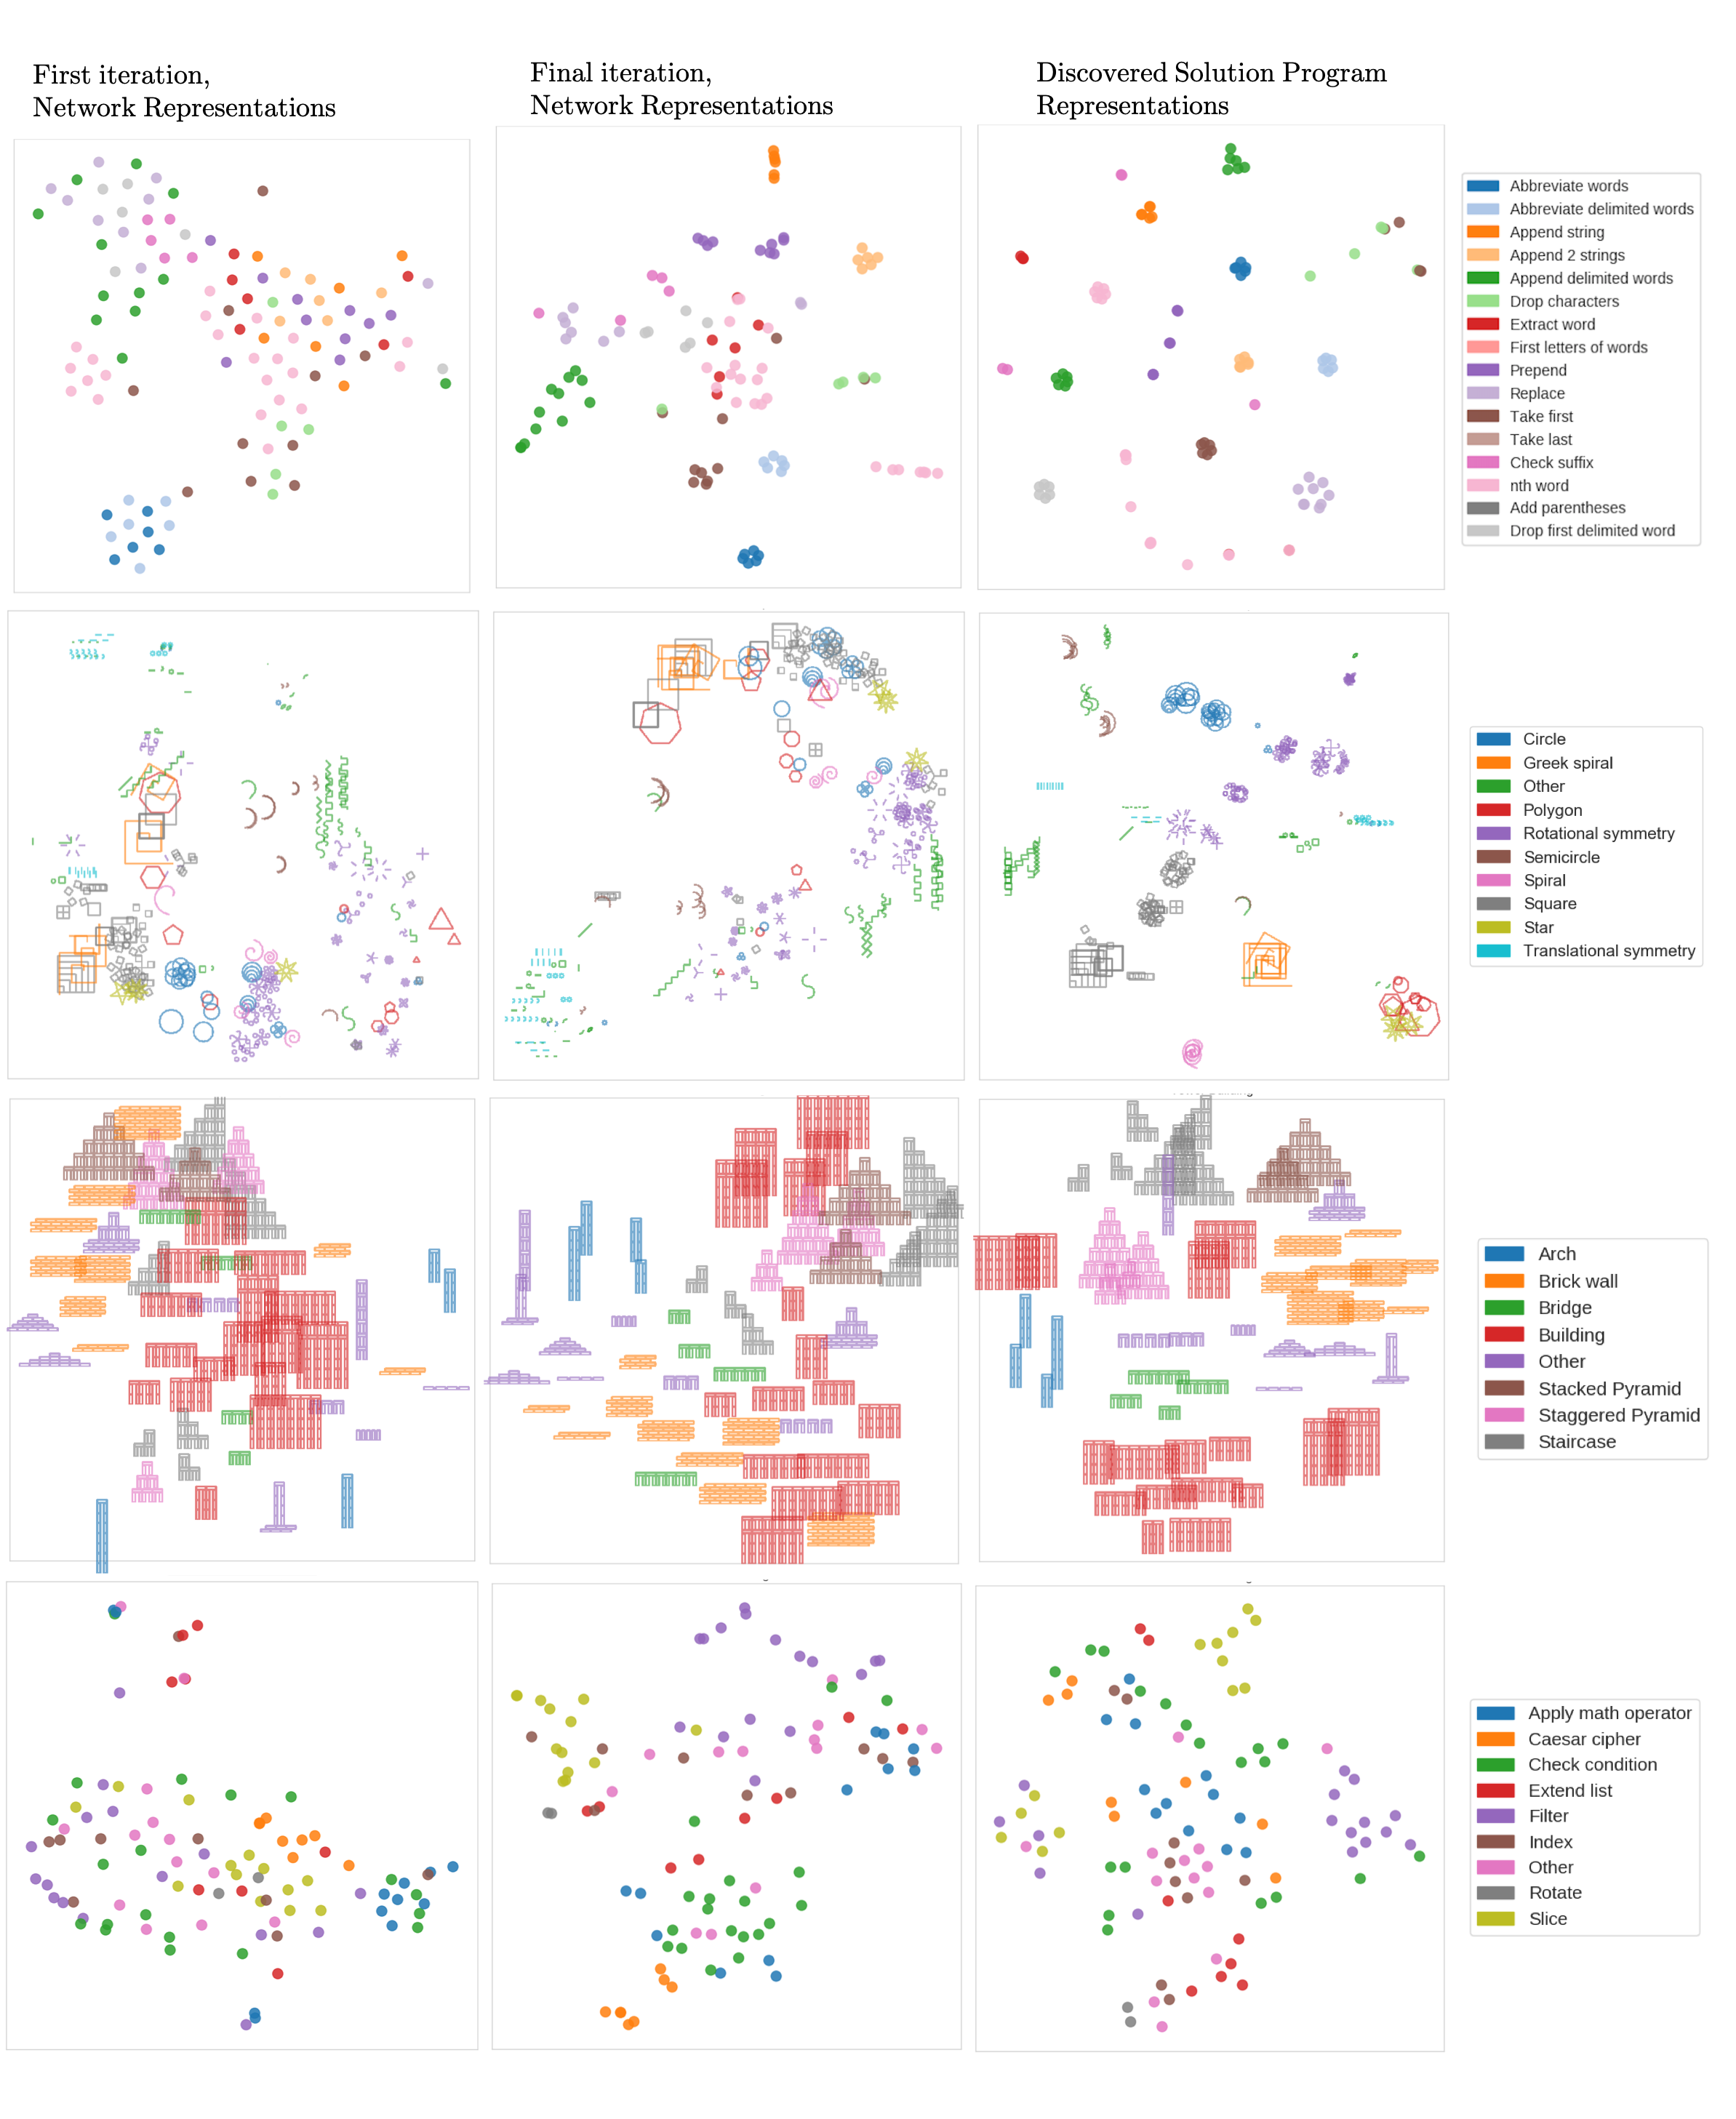
\includegraphics[width = \textwidth]{figures/all_tsne.png}
  \caption{}\label{allTSNE}
\end{figure}

\subsection{LOGO Graphics Experiment}

We apply our system to 160 LOGO graphics tasks, split 50/50 test/train (Figure~\ref{everyLogoTask}).
For each task of the agent must write a program that moves a simulated pen across the canvas,
with the goal of drawing the target image, as measured by pixel level similarity.

We initially provide our agent with two control flow primitives: \code{for} (a `for` loop), and \code{get/set}, which gets and saves the current state of the agent's pen, executes a block of code, and then restores the state to its previous value. We provide two different drawing primitives: \code{move}, which takes as input both a distance and angle, and moves the pen forward by that distance and rotates by that angle, and \code{pen-up}, which lifts up the pen and then executes a block of code \emph{without} placing down ink on the canvas.

These programs are imperative (produce a sequence of actions) rather than purely functional (calculate a stateless mapping).
The \system infrastructure only supports purely functional $\lambda$-calculus programs.
To embed imperative routines within this framework,
we model imperative routines using a state monad~\cite{wadler1990comprehending} and encode each imperative action in a continuation passing style where each imperative primitive takes as input the actions to execute afterwards (i.e., the continuation),
and the program as a whole takes as input a final no-op continuation.
This continuation passing set up allows the program synthesizer to not need the monadic `bind' operator to sequence chains of commands.
To be concrete, our imperative primitives have the following types:

\begin{tabular}{l}
  \code{move} : \code{distance}$\to$\code{angle}$\to$\code{State ()}$\to$\code{State ()}\\
  \code{pen-up} : \code{(State ()$\to$State ())}$\to$\code{State ()}$\to$\code{State ()}\\
  \code{for} : \code{int$\to$(State ()$\to$State ())}$\to$\code{State ()}$\to$\code{State ()}\\
  \code{get/set} : \code{(State ()$\to$State ())}$\to$\code{State ()}$\to$\code{State ()}
\end{tabular}

and each synthesized program has type \code{State ()}$\to$\code{State ()}. We additionally provide the agent with natural numbers (1 through 9), arithmetic operations (addition/subtraction/multiplication/division), unit distances and angles (1 meter and $2\pi$ radians), and special values $\infty$ (approximated as $20$) and $\epsilon$ (approximated as $1/20$). We distinguish distances and angles in the type system, only allowing a distance/angle to be added/subtracted with another object that is also a distance/angle, and only allowing multiplication/division by unitless scalars. This trick requires no modification of the underlying \system software, and is a standard way of embedding units and dimensions within a type system~\cite{fsunits}.


\begin{figure}
  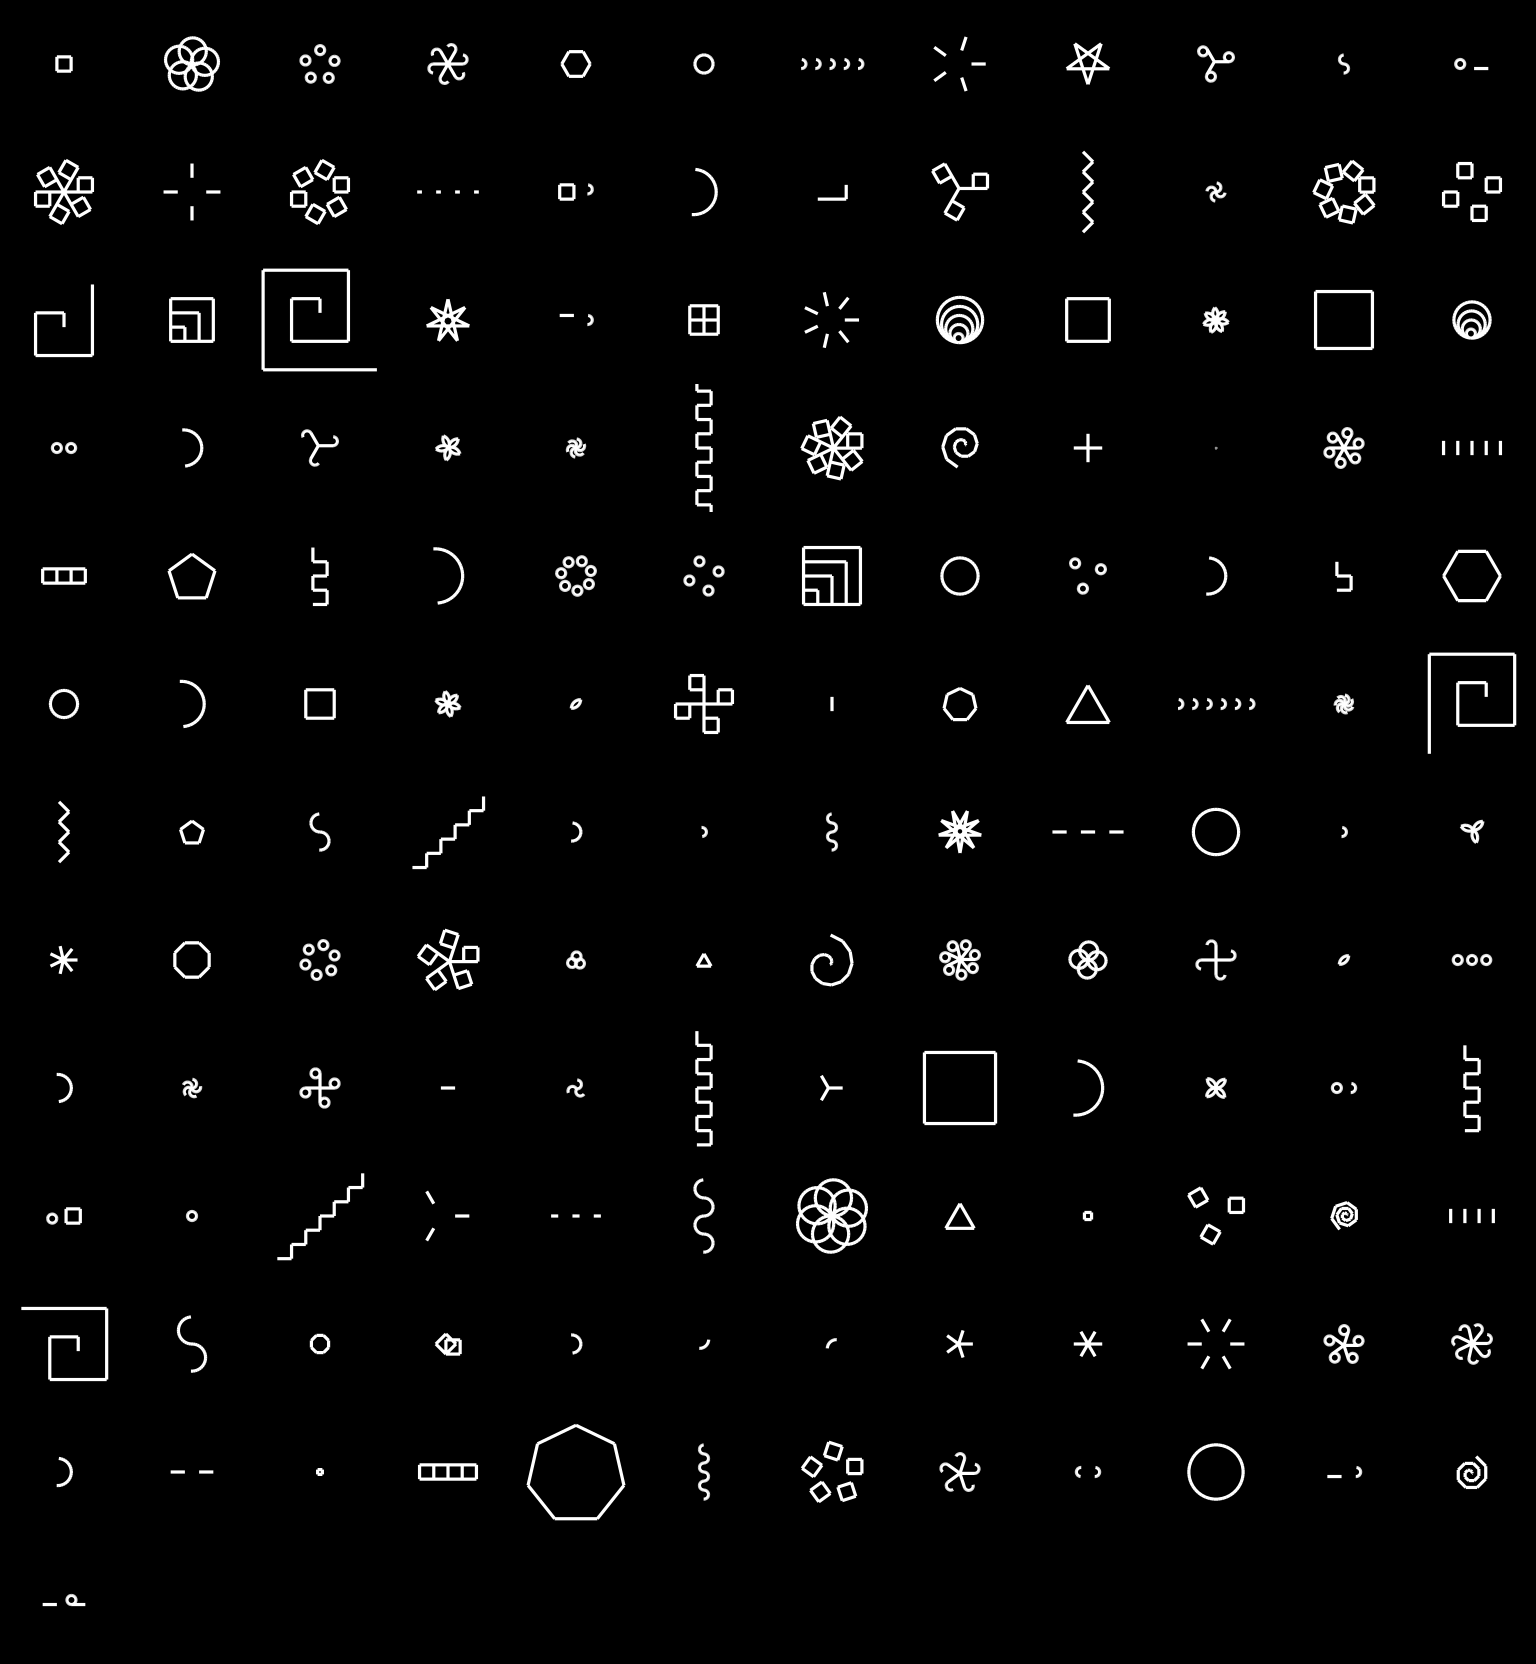
\includegraphics[width = \textwidth]{figures/fullLogo.png}
  \caption{Full set of LOGO graphics tasks that we apply our system to}\label{everyLogoTask}
\end{figure}

\subsection{Tower Building Experiment}
We apply our system to 112 tower building tasks (Figure~\ref{everyTowerTask}), split 50/50 test/train.
We use the same monadic, continuation-passing encoding of imperative programs as we used for LOGO graphics,
and include the exact same control flow primitives.
Rather than moving a pen over a canvas, the agent here moves a simulated hand left/right over a 2D tower building stage, and has at its disposal an unlimited supply of horizontal and vertical blocks.
All coordinates are discretized.
Horizontal blocks have size 6x2 and vertical blocks have size 2x6.
The state of the simulated hand maintains both its position (a single discrete scalar) and its orientation (a single boolean, either facing left are facing right).
We include two domain specific primitives for adjusting the position of the hand: \code{move}, which takes as input a scalar $d$ and moves the hand forward  by distance $d$,
and \code{reverse},
which flips the orientation of the hand.
The agent has two additional domain specific primitives for dropping a horizontal/vertical block at the current position of the hand.


\begin{figure}
  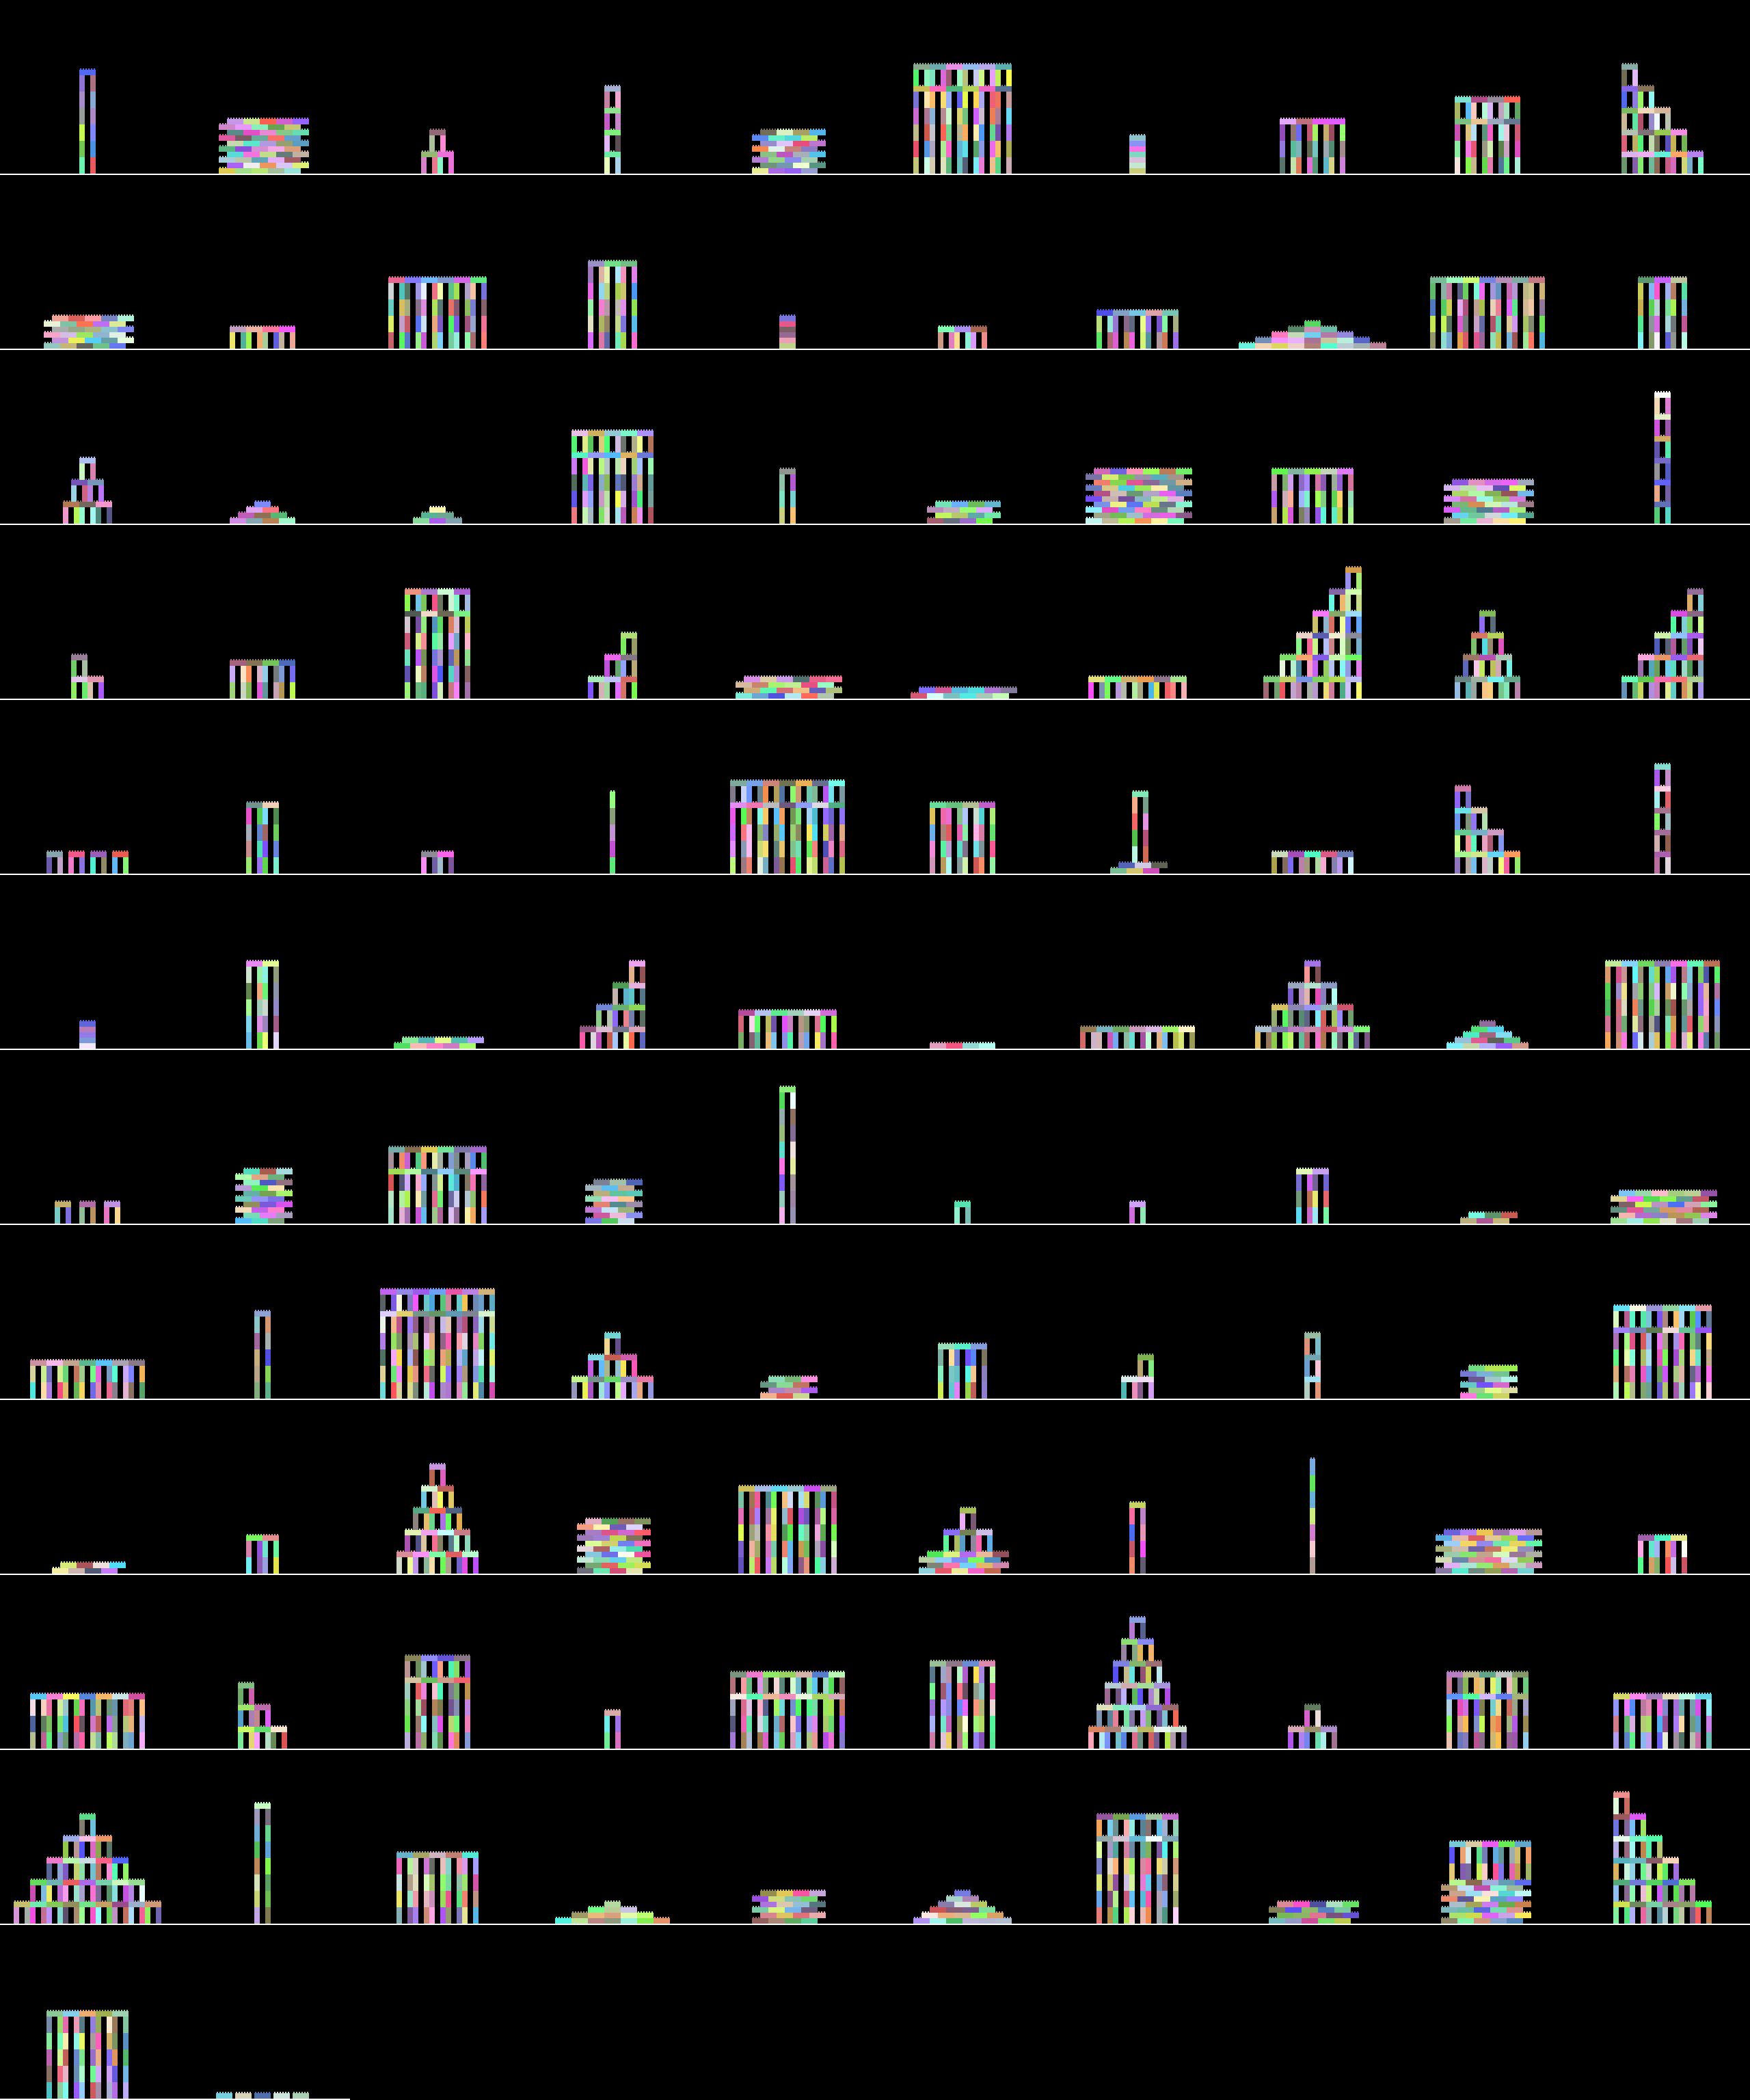
\includegraphics[width = \textwidth]{figures/fullTower.png}
  \caption{Full set of tower building tasks that we apply our system to}\label{everyTowerTask}
\end{figure}

\subsection{Learning from Scratch: Tasks and Library}\label{appendixMcCarthy}

We gave our system the following primitives: \code{if}, \code{=},
\code{>}, \code{+}, \code{-}, \code{0}, \code{1}, \code{cons},
\code{car}, \code{cdr}, \code{nil}, and \code{is-nil}, all of which
are present in some form in McCarthy's 1959
Lisp~\cite{mccarthy1960recursive}.\footnote{McCarthy's first version
  of Lisp used \code{cond} instead of \code{if}. Because we are using
  a typed language, we instead used \code{if}, because Lisp-style
  \code{cond} is unwieldy to express as a function in typed
  languages.}  We furthermore allowed functions to call themselves,
which we modeled using the Y combinator.  We did not use the
recognition model for this experiment: a bottom-up pattern recognizer
is of little use for acquiring this abstract knowledge from less than
two dozen problems.

Figure~\ref{learningFromScratch} shows the full set of tasks and the learned library.
\begin{figure}  \newcommand{\helpSize}{0.25cm}
  \begin{tabular}{ll}\toprule
    \normalsize \rotatebox[origin=c]{90}{\pop{Programs} \& Tasks}&%&\normalsize \popp{DSL}\\\midrule

    \begin{tabular}{ll}      
      \begin{tabular}{l}
        \code{[1\, 9]}$\to $\code{2}\\
        \code{[5\, 3\, 8]$\to$3}\\
        \blueCode{$f(\ell) = $($f_5$ $\ell$)}
      \end{tabular}&
      \begin{tabular}{l}
        \code{[[2 1]\, []]}$\to $\code{[2 0]}\\
        \code{[[] [] [9 8 9 9]]$\to$[0 0 4]}\\
        \blueCode{$f(\ell) = $($f_2$ $f_5$ $\ell$)}
      \end{tabular}\\\\

      \begin{tabular}{l}
        \code{[0 1 1 0 0]$\to$[1 1]}\\
        \code{[9 0 8]$\to$[9\, 8]}\\
        \blueCode{$f(\ell) = $($f_3$ (eq? 0) $\ell$)}        
      \end{tabular}&
      \begin{tabular}{l}
        \code{[1 -1 0 2]$\to$[1 2]}\\
        \code{[9 -5 5 0 8]$\to$[9 5 8]}\\
        \blueCode{$f(\ell) = $($f_3$ (gt? 1) $\ell$)}        
      \end{tabular}\\\\

      \begin{tabular}{l}
        \code{[2\, 1\, 4]$\to$[2\, 1\, 4\, 0]}\\
        \code{[9\, 8]$\to$[9\, 8\, 0]}\\
        \blueCode{$f(\ell) = $($f_0$ cons $\ell$ (cons 0 nil))}
      \end{tabular}&


      \begin{tabular}{l}
        \code{[2\, 1\, 4]$\to$[2\, 1]}\\
        \code{[9\, 8]$\to$[9]}\\
        \blueCode{$f(\ell) = $($f_6$ cdr ($\lambda$ (z) (empty? (cdr z))) $\ell$)}
      \end{tabular}\\\\

      \begin{tabular}{l}
        \code{[2\, 5\, 6\, 0\, 6]$\to$19}\\
        \code{[9\, 2\, 7\, 6\, 3]$\to$27}\\
        \blueCode{$f(\ell) = $($f_0$ + $\ell$ 0)}
      \end{tabular}&

      \begin{tabular}{l}
        \code{[4\, 2\, 6\, 4]$\to$[8\, 4\, 12\, 8]}\\
        \code{[2\, 3\, 0\, 7]$\to$[4\, 6\, 0\, 14]}\\
        \blueCode{$f(\ell) = $($f_2$ ($\lambda$ (x) (+ x x)) $\ell$)}
      \end{tabular}\\\\

      \begin{tabular}{l}
        \code{[4\, 2\, 6\, 4]$\to$[-4\, -2\, -6\, -4]}\\
        \code{[2\, 3\, 0\, 7]$\to$[-2\, -3\, -0\, -7]}\\
        \blueCode{$f(\ell) = $($f_2$ (- 0) $\ell$)}
      \end{tabular}&
      \begin{tabular}{l}
        \code{[4\, 2\, 6\, 4]$\to$[5\, 3\, 7\, 5]}\\
        \code{[2\, 3\, 0\, 7]$\to$[3\, 4\, 1\, 8]}\\
        \blueCode{$f(\ell) = $($f_2$ (+ 1) $\ell$)}
      \end{tabular}\\\\

      \begin{tabular}{l}
        \code{[1\, 5\, 2\, 9]}$\to$\code{[1\, 2]}\\
        \code{[3\, 8\, 1\, 3\, 1\, 2]}$\to$\code{[3\, 1\, 1]}\\
        \blueCode{$f(\ell) = $($f_6$ ($\lambda$ (l) (cdr (cdr l))) empty? $\ell$}
      \end{tabular}&
      
      \begin{tabular}{l}
        \code{3$\to $[0\, 1\, 2]}\\
        \code{2$\to $[0\, 1]}\\
        \blueCode{$f(n) = $($f_9$ $n$)}
      \end{tabular}\\\\

      
      \begin{tabular}{l}
        \code{3$\to $[0\, 1\, 2\, 3]}\\
        \code{2$\to $[0\, 1\, 2]}\\
        \blueCode{$f(n) = $($f_9$ (+ 1 $n$))}
      \end{tabular}&
      \begin{tabular}{l}
        \code{[9 2]$\to $[9 9 2 2]}\\
        \code{[1 2 3 4]$\to $[1 1 2 2 3 3 4 4]}\\
        \blueCode{$f(l) = $($f_0$ ($\lambda$ (a x) (cons x (cons x a))) l nil)}
      \end{tabular}\\\\


      \begin{tabular}{l}
        \code{0, [9 2 3]$\to $9}\\
        \code{3, [0 2 8 4 5 6]$\to $4}\\
        \blueCode{$f($n$,$l$) = $($f_{10}$ l n)}
      \end{tabular}&
      \begin{tabular}{l}
        \code{1, [9 2 3]$\to $9}\\
        \code{4, [0 2 8 1 5 6]$\to $1}\\
        \blueCode{$f($n$,$l$) = $($f_{10}$ l (+ 1 n))}
      \end{tabular}\\\\
      \begin{tabular}{l}
        \code{3$\to $[-3 -2 -1]}\\
        \code{4$\to $[-4 -3 -2 -1]}\\
        \blueCode{$f($n$) = $($f_{8}$ 0 n)}
      \end{tabular}&
      \begin{tabular}{l}
        \code{2$\to $[2 1]}\\
        \code{4$\to $[4 3 2 1]}\\
        \blueCode{$f($n$) = $($f_{8}$ 0 (- 0 n))}
      \end{tabular}      
    \end{tabular}
    \\\midrule 
    \rotatebox[origin=c]{90}{\normalsize \popp{Library}}&
    \begin{tabular}{ll}
      \begin{tabular}{l}
        \popp{\code{$f_0($f$,$l$,$x$)\,=\,$(if (empty? l) x}}\\
        \phantom{\code{$f_0($f$,$l$,$x$)\,=\,$(if }}}\popp{\code{(f (car l) ($f_0$ (cdr l))))}}\\
          \hspace{\helpSize}($f_0$: \emph{fold})
      \end{tabular}&
      \begin{tabular}{l}
        \popp{\code{$f_1($p$,$f$,$n$,$x$)\,=\,$(if (p x) nil}}\\
        \phantom{\code{$f_1($f$,$l$,$x$)\,=\,$(if }}}\popp{\code{(cons (f x) ($f_1$ (n x))))}}\\
          \hspace{\helpSize}($f_1$: \emph{unfold})
      \end{tabular}\\
      \begin{tabular}{l}
        \greenCode{$f_2($f$,$l$)\,=\,$($f_0$ nil l ($\lambda$ (x a) (cons (f x) a)))}\\
        \hspace{\helpSize}($f_2$: \emph{map})
      \end{tabular}&
      \begin{tabular}{l}
                  \greenCode{$f_3($f$,$l$)\,=\,$($f_0$ nil l ($\lambda$ (x a) (if (f x) a (cons x a))))}\\
          \hspace{\helpSize}($f_3$: \emph{filter})
      \end{tabular}\\
      \begin{tabular}{l}
        \greenCode{$f_4($f$,$p$,$n$)\,=\,$($f_1$ p f (+ 1) n)}\\
        \hspace{\helpSize}($f_4$: \emph{count upward until predicate holds})
      \end{tabular}&
      \begin{tabular}{l}
        \greenCode{$f_5($l$)\,=\,$($f_0$ ($\lambda$ (a x) (+ 1 a)) l 0)}\\
        \hspace{\helpSize}($f_5$: \emph{length})
      \end{tabular}\\
      \begin{tabular}{l}
        \greenCode{$f_6($n$,$p$,$l$)\,=\,$($f_1$ p n car l)}\\
        \hspace{\helpSize}($f_6$: \emph{specialization of unfold})
      \end{tabular}&
      \begin{tabular}{l}
        \greenCode{$f_7($p$)\,=\,$($f_4$ ($\lambda$ (x) x) p 0)}\\
        \hspace{\helpSize}($f_7$: \emph{count upward from 0 until predicate holds})
      \end{tabular}\\
      \begin{tabular}{l}
        \greenCode{$f_8($n$,$m$)\,=\,$($f_4$ ($\lambda$ (x) (- n x)) (eq? 0) m)}\\
        \hspace{\helpSize}($f_7$: \emph{count downwards})
      \end{tabular}&
      \begin{tabular}{l}
        \greenCode{$f_9($n$)\,=\,$($f_7$ (eq? n))}\\
        \hspace{\helpSize}($f_9$: \emph{range})
      \end{tabular}\\
      \begin{tabular}{l}
        \greenCode{$f_{10}($l$,$n$)\,=\,$(car ($f_0$ ($\lambda$ (a x) (cdr a)) ($f_9$ n) l))}\\
        \hspace{\helpSize}($f_{10}$: \emph{index})
      \end{tabular}&
      
      
      
    \end{tabular}
%%     \begin{tabular}{l}
%%         \popp{\code{$f_1($i$,$l$)\,=\,$(if (= i 0) (car l)}}\\
%%       \phantom{\code{$f_1($f$,$l$,$x$)\,=\,$(if}}}\popp{\code{($f_1$ (- i 1) (cdr l))))}}\\
%%         \hspace{\helpSize}($f_1$: \emph{index})\\

%%         \greenCode{$f_4(\ell)$\,=\,(if (empty? $\ell$) 0 (+ 1 ($f_4$ (cdr $\ell$)))))}\\
%%         \hspace{\helpSize}($f_4$: \emph{length})\\
%%         \greenCode{$f_5(\code{f},\code{m},\code{n})$\,=\,($f_0$ (= m) f (+ 1) n)}\\
%%         \hspace{\helpSize}($f_5$: \emph{generalization of range})

%% %        -0.222777	int -> int -> list(int)	#(lambda (lambda (fix1 $0 (lambda (lambda (#(lambda (lambda (lambda (if $0 empty (cons $1 $2))))) (map (lambda (#(+ 1) $0)) ($1 (#(lambda (- $0 1)) $0))) 0 (eq? $0 $3)))))))

%%       \end{tabular}
    %% : (lambda (#(#(lambda (lambda (lambda (lambda (fix1 $0 (lambda (lambda (if (empty? $0) $3 ($4 ($5 $0) ($1 (cdr $0))))))))))) (lambda (car $0))) (lambda (lambda (+ $0 $1))) 0 $0))
    %% (lambda (lambda (lambda (lambda (fix1 $0 (lambda (lambda (#(lambda (lambda (lambda (if $0 empty (cons $1 $2))))) ($1 ($3 $0)) ($4 $0) ($5 $0)))))))))
    %% (lambda (lambda (fix1 $0 (lambda (lambda (#(lambda (lambda (lambda (if $0 empty (cons $1 $2))))) (#(lambda (lambda (fix1 $0 (lambda (lambda (if (empty? $0) empty (cons ($3 (car $0)) ($1 (cdr $0))))))))) (lambda (#(+ 1) $0)) ($1 (#(lambda (- $0 1)) $0))) 0 (eq? $0 $3)))))))
    \\\bottomrule 
    \end{tabular}
  \caption{Bootstrapping a standard library of functional programming routines, starting from recursion along with primitive operations found in 1959 Lisp. Complete set of tasks and learned DSL shown. Learned DSL components are numbered in the order that they are learned, \emph{i.e.}, the agent first learns fold, then unfold, then uses fold to define map, etc.}\label{learningFromScratch}
  \end{figure}


%% \begin{figure}
%%   \begin{tikzpicture}
%%     \node at (0,0) (d){DSL};
%%     \node at ([yshift = -2cm]d) (t){$\text{Task}$};

%%     \node at ([xshift = 2cm]t) (nn){
%%       \begin{tikzpicture}[x=2.5cm,y=1.25cm,transform canvas={scale=0.2,shift={+(-1,2.5)}}]
%%         \tikzstyle{neuron}=[circle,fill=blue!50,minimum size=20pt]
%%         \fill[fill=white] (-0.25,-0.5) rectangle (2.25,-4.5);
%%         \node[rectangle] at (1,1) {};
%%         \foreach \name / \y in {1,...,4}
%%             \node[neuron] (I-\name) at (0,-\y) {};
%%         \foreach \name / \y in {1,...,3}
%%             \node[neuron] (H-\name) at (1,-\y-0.5) {};
%%         \foreach \name / \y in {1,...,4}
%%             \node[neuron] (O-\name) at (2,-\y) {};
%%         \foreach \source in {1,...,4}
%%             \foreach \dest in {1,...,3}
%%                 \draw [-latex] (I-\source) -- (H-\dest);
%%         \foreach \source in {1,...,3}
%%             \foreach \dest in {1,...,4}
%%                 \draw [-latex] (H-\source) -- (O-\dest);
%%       \end{tikzpicture}
%%     };
%%     \node[align = center, text width = 1cm] at ([yshift = 0.6cm]nn.north) {\baselineskip=0pt \small Recognition model\par};
%%     \draw [->] (t.east) -- ([xshift = -0.5cm]nn.west);

%%     \node[draw,rounded corners, inner sep = 10] at ([xshift = 4.2cm,yshift = -1cm]) (s){Search};
%%     \node at ([xshift=-7pt,yshift=5pt]s.north west) {$\mathcal{D}$};

%%     \draw [->] ([xshift = 0.5cm]nn.east) -- ([yshift = -0.25cm]s.west);
%%     \draw [->,rounded corners] (d.east) -- ([yshift = 2cm]nn.center) -- ([yshift = 0.25cm]s.west);

%%     \node[align=left] at (7,-1) (f) {Frontier\\{\small (set of programs)}};
%%     \draw [->  ] (s.east) -- (f.west);

%%     \draw [->  ,rounded corners] (t.south) -- ([yshift = -0.5cm]t.south) -- ([yshift = -0.5cm] s.south |- t.south) -- (s.south);
%%     \node at ([xshift = 0.5cm,yshift = -0.75cm]s.south) {Spec};

%%     \node at (4,-3.5) {\textbf{\textsc{Wake: Problem Solving}}};
    
    
%%   \end{tikzpicture}

%%   \vspace{1cm}
  
  

%%   \begin{tikzpicture}
%%     \node at (0,0) (f1){Frontier$_1$};
%%     \node at ([yshift = -1cm]f1.south) (f2){Frontier$_2$};
%%     \node at ([yshift = -1cm]f2.south) (f3){Frontier$_3$};

%%     \node at ([xshift = 2cm]f1.east) (p1){program$_1$};
%%     \node at ([xshift = 2cm]f2.east) (p2){program$_2$};
%%     \node at ([xshift = 2cm]f3.east) (p3){program$_3$};


%%     \draw [->,squiggle ] (f1.east) -- node[above]{\small sample} (p1.west);
%%     \draw [->,squiggle ] (f2.east) -- node[above]{\small sample} (p2.west);
%%     \draw [->,squiggle ] (f3.east) -- node[above]{\small sample} (p3.west);
    
%%     \node at ([xshift = 1.5cm]p1.east) (t1){task$_1$};
%%     \node at ([xshift = 1.5cm]p2.east) (t2){task$_2$};
%%     \node at ([xshift = 1.5cm]p3.east) (t3){task$_3$};

%%     \node at ([yshift = -0.5cm]p3.south) {\textsc{\textbf{Sleep-R: Experience Replay}}};
%%   \end{tikzpicture}

%%   \begin{tikzpicture}
%%     \node[align=center] at (0,0) (d){DSL\\$(\mathcal{D},\theta)$};
%%     \node at ([xshift = 3cm]d.east) (p2){program};
%%     \node at ([yshift = 1.5cm]p2) (p1){program};
%%     \node at ([yshift = -1.5cm]p2) (p3){program};


%%     \draw[squiggle,-> ] (d.east) -- node[above]{\small sample} (p2.west);
%%     \draw[squiggle,-> ] (d.east) -- (p1.west);
%%     \draw[squiggle,-> ] (d.east) -- (p3.west);

%%     \node at ([xshift = 2cm]p1.east) (t1){task};
%%     \node at ([xshift = 2cm]p2.east) (t2){task};
%%     \node at ([xshift = 2cm]p3.east) (t3){task};
%%     \draw [-> ] (p1.east) -- node[above]{\small execute} (t1.west);
%%     \draw [-> ] (p3.east) -- node[above]{\small execute} (t3.west);
%%     \draw [-> ] (p2.east) -- node[above]{\small execute} (t2.west);

%%     \node at ([yshift = -0.5cm]p3.south) {\textsc{\textbf{Sleep-R: Dreaming}}};
%%   \end{tikzpicture}
  
%%   \vspace{2cm}
  
%%   \begin{tikzpicture}
%%     \node at (0,0) (f1){Frontier$_1$};
%%     \node at ([yshift = -1cm]f1.south) (f2){Frontier$_2$};
%%     \node at ([yshift = -0.7cm]f2.south) (ff){\textbf{$\vdots$}};
%%     \node at ([yshift = -1.2cm]f2.south) (ff){\textbf{$\vdots$}};
%%     \node at ([yshift = -1cm]ff.south) (f3){Frontier$_N$};

%%     \node(c)[rectangle, rounded corners, draw, minimum width = 3cm, minimum height = 6cm, anchor = north west] at (2,1) {};
%%     \node[anchor=north] at (c.north) {Compression};

%%     \draw [-> ] (f1.east) -- (c.west|-f1.east);
%%     \draw [-> ] (f2.east) -- (c.west|-f2.east);
%%     \draw [-> ] (f3.east) -- (c.west|-f3.east);

%%     \node[right](d) at ([xshift = 1.2cm,yshift = 0.7cm]c.east) {DSL $\mathcal{D}$};
%%     \node[right](t) at ([xshift = 1.2cm,yshift = -0.7cm]c.east) {Weights $\theta$};
%%     \draw [-> ] (c.east) -- (d.west);
%%     \draw [-> ] (c.east) -- (t.west);

%%     \node at (c.center) {
%% \begin{tikzpicture}[scale=0.7]
%%     %% \node[rotate=30] at (-2,0) {\begin{tabular}{c}
%%     %%     \footnotesize Program:\\
%%     %%     \code{($\lambda$ (x) (+ (- x) 1))}
%%     %% \end{tabular}};
%%     %\node at (,0.5) {\code{cons}};
%% %    \node [rotate=90] at (-2.3,-0.5) {\small program};
    
%%           \node(l1) at (0,0) {};
%%   \node[color=pop3](p1) at (-1,-1) {\code{+}};
%%   \node[color=pop3](n1) at (0.7,-0.9) {\code{1}};
%%   \node(x1) at (0,-1) {\code{1}};
%%   \draw[color=pop3] (l1.south) -- (p1.north);
%%   \draw[color=pop3] (l1.south) -- (n1.north);
%%   \draw[color=pop3] (-0.5,-0.45) -- (x1.north);

%%   \node(t) at (-0.5,0.5) {};
%%   \draw (l1.south) -- (t.south);
%%   \node(c) at (-1.5,-0.2) {\code{cons}};
%%   \draw (t.south) -- (c.north);
  
%% %    \draw  (l1.south) -- (-0.5,0.5);

%%   %% \node(c) at (-0.5,-1.5) {\code{-}};
%%   %% \node(z) at (0.5,-1.5) {\code{x}};

%%   %% \draw (0,-1) -- (c.north);
%%   %% \draw (0,-1) -- (z.north);
  
%%   \begin{scope}[shift={(-1,-2.5)}]
%%       \node(l1) at (0,0) {};
%%   \node[color=pop3](p1) at (-1,-1) {\code{+}};
%%   \node[color=pop3](n1) at (0.7,-0.9) {\code{1}};
%%   %\node(x1) at (0,-1) {};
%%   \draw[color=pop3] (l1.south) -- (p1.north);
%%   \draw[color=pop3] (l1.south) -- (n1.north);
%%   \draw[color=pop3] (-0.5,-0.45) -- (0,-1);


%%   \node(c) at (-0.5,-1.5) {\code{car}};
%%   \node(z) at (0.5,-1.5) {\code{z}};

%%   \draw (0,-1) -- (c.north);
%%   \draw (0,-1) -- (z.north);

%% %  \node [rotate=90] at (-2.3,-0.7) {\small program};
  
%%   \end{scope}

%% \begin{scope}[shift={(0,-5)}]
%%   \node[pop3](p1) at (-1,-1) {\code{+}};
%%   \node[pop3](n1) at (0.8,-0.7) {\code{1}};
%%   \node[pop3](a) at (0,-1) {\code{ }};
%%   %\node(x1) at (0,-1) {};
%%   \draw[pop3] (0,0) -- (p1.north);
%%   \draw[pop3] (0,0) -- (n1.north);
%%   \draw[pop3] (-0.55,-0.4) -- (a.north);
%% %  \node [rotate=90] at (-2.3,-0.7) {\small fragment};

%%   \end{scope}

%% \end{tikzpicture}
%%     };

%%     \node at ([yshift=-2.5cm,xshift = 4cm]c.south) {\textsc{\textbf{Sleep-G: Memory Consolidation}}};

%%     \end{tikzpicture}
%% \end{figure}

%% \begin{table*}%[t!]
%%   \makebox[\textwidth][c]{
%%     \scriptsize
%%   \tabcolsep=4pt
%%   \renewcommand\code\texttt
%%   \renewcommand\codechar[1]{\texttt{"#1"}}
%%   \newcommand{\helpSize}{0.25cm}
%%   \begin{tabular}{cccc}
%%     \toprule
%%     &{\normalsize Symbolic regression}&{\normalsize Laws of motion}&\\\midrule
%%     \rotatebox[origin=c]{90}{\normalsize \pop{Programs} \& Tasks}&{\tabcolsep=7pt
%%     \begin{tabular}{cc}
%%       
\includegraphics[width = 3em]{figures/functions/4.png}&
%%       
\includegraphics[width = 3em]{figures/functions/146}\\
%%       \pop{\code{$f($x$) = $($f_1$ x)}}&    \pop{\code{$f($x$) = $($f_6$ x)}}\\
%%       ~\\
%%       
\includegraphics[width = 3em]{figures/functions/112.png}&
%%         
\includegraphics[width = 3em]{figures/functions/92.png}
%%       \\
%%       \pop{\code{$f($x$) = $($f_4$ x)}}&    \pop{\code{$f($x$) = $($f_3$ x)}}\\

%%     \end{tabular}
%%     }
%%     &
%%     \begin{tabular}{cc}
%%       \includegraphics[width = 15em]{figures/massOnSpring.png} &
%%             \includegraphics[width = 15em]{figures/planets.png}
%%       \\
%%       \begin{tabular}{l}
%%               \blueCode{$f($o,$\Delta) = $($f_3$ o $\Delta$}\\
%%       \hspace{1cm}\blueCode{(- (* $k$ (pos o))}\\
%%       \hspace{1cm}\phantom{\code{(- }}\blueCode{(* $-9.8$ $\hat{x}$)))}\\
%%       \end{tabular}&
%%       \begin{tabular}{l}
%%               \blueCode{$f($a,b,$\Delta) = $($f_3$ a $\Delta$}\\
%%       \hspace{1cm}\blueCode{(/ (* $G$ (mass a) (mass b))}\\
%%       \hspace{1cm}\phantom{\code{(- }}\blueCode{(square (- (pos a) (pos b)))))}\\
%%         \end{tabular}
%%       \end{tabular}
%%     &

%%     ~\\
%%     \midrule
%%     \rotatebox[origin=c]{90}{\normalsize \popp{DSL}}&
%%       \begin{tabular}{l}
%%     \popp{$f_0($\code{x}$)\,=\,$\code{(+ x real)}}\\
%%     \popp{$f_1($\code{x}$)\,=\,$\code{($f_0$ (* real x))} }\\
%%     \popp{$f_2($\code{x}$)\,=\,$\code{($f_1$ (* x (}$f_0$\code{ x)))}}\\
%%     \popp{$f_3($\code{x}$)\,=\,$\code{($f_0$ (* x (}$f_2$\code{ x)))}}\\
%%     \popp{$f_4($\code{x}$)\,=\,$\code{($f_0$ (* x (}$f_3$\code{ x)))}}\\
%%     \hspace{\helpSize}\emph{($f_4$: 4th order polynomial)}\\
%%     \popp{$f_5($\code{x}$)\,=\,$\code{(/ real x)}}\\
%%     \popp{$f_6($\code{x}$)\,=\,$\code{($f_5$ ($f_0$ x))}}\\
%%     \hspace{\helpSize}\emph{($f_6$: rational function)}\\

%%   \end{tabular}
%%       &
%%       \begin{tabular}{l}
%%         \greenCode{$f_0($\code{o},$\Delta)\, = \,$(set-pos o (+ (pos o) (* $\Delta$ (vel o))))}\\
%%         \hspace{\helpSize}\emph{($f_0$: integrates position)}\\
%%         \greenCode{$f_1($\code{o},\code{a},$\Delta)\, = \,$(set-vel o (+ (vel o) (* $\Delta$ a)))}\\
%%         \hspace{\helpSize}\emph{($f_1$: integrates velocity)}\\
%%         \greenCode{$f_2($\code{o},\code{F}$)\, = \,$(/ F (mass o))}\\
%%         \hspace{\helpSize}\emph{($f_2$: Newton's second law)}\\
%%         \greenCode{$f_3($\code{o},$\Delta$,\code{F}$)\, = \,$($f_0$ o $\Delta$ ($f_1$ o ($f_2$ o F) $\Delta$))}\\
%%         \hspace{\helpSize}\emph{($f_3$: applies Newton's second law and integrates)}
        
%%         \end{tabular}


%% &


%%   \\\bottomrule\\
%% \end{tabular}}\vspace{-0.5cm} 
%% \caption{Top: Tasks from three domains we apply our algorithm to, each followed by the programs \system discovers for them. Bottom: Several examples from learned DSL. Notice that learned DSL primitives can call each other, and that \system rediscovers higher-order functions like \code{filter} ($f_1$ under List Functions)}\label{initialExampleDSL}%\vspace{-0.5cm}
%% \end{table*}

\subsection{Learned DSLs}
Here we present representative DSLs learned by our model. DSL primitives
discovered by the algorithm are prefixed with \lstinline!#!.
Variables are prefixed with \lstinline!$!, and we adopt De Bruijn indices to
model bound variables~\cite{pierce}.


\lstset{
  basicstyle=\footnotesize,
  escapechar=@,
  breaklines=true,
  breakatwhitespace=true,
  postbreak=\mbox{\textcolor{red}{$\hookrightarrow$}\space}
}


\subsubsection{List processing}
\begin{lstlisting}
#(@$\lambda$@ (@$\lambda$@ (map (@$\lambda$@ (index $0 $2)) (range ($0 (+ 1))))))
#(@$\lambda$@ (@$\lambda$@ (fold $1 empty (@$\lambda$@ (@$\lambda$@ (if ($2 $1) (cons $1 $0) $0))))))
#(+ 1 (+ 1 1))
#(@$\lambda$@ (@$\lambda$@ (fold $1 (cons $0 empty) (@$\lambda$@ (@$\lambda$@ (cons $1 $0))))))
#(+ 1 #(+ 1 (+ 1 1)))
#(@$\lambda$@ (map (@$\lambda$@ (if ($1 $0) (+ $0 1) 0))))
#(@$\lambda$@ (cdr (cdr $0)))
#(@$\lambda$@ (@$\lambda$@ (fold (#(@$\lambda$@ (cdr (cdr $0))) (#(@$\lambda$@ (cdr (cdr $0))) $1)) $0 (@$\lambda$@ (@$\lambda$@ (cdr (#(@$\lambda$@ (@$\lambda$@ (fold $1 (cons $0 empty) (@$\lambda$@ (@$\lambda$@ (cons $1 $0)))))) $0 (car $0))))))))
#(@$\lambda$@ (car (#(@$\lambda$@ (@$\lambda$@ (fold $1 empty (@$\lambda$@ (@$\lambda$@ (if ($2 $1) (cons $1 $0) $0)))))) $0 (@$\lambda$@ (empty? (#(@$\lambda$@ (@$\lambda$@ (fold $1 empty (@$\lambda$@ (@$\lambda$@ (if ($2 $1) (cons $1 $0) $0)))))) $1 (@$\lambda$@ (gt? $0 $1))))))))
#(@$\lambda$@ (@$\lambda$@ (length (#(@$\lambda$@ (@$\lambda$@ (fold $1 empty (@$\lambda$@ (@$\lambda$@ (if ($2 $1) (cons $1 $0) $0)))))) $1 (@$\lambda$@ (eq? $0 $1))))))
#(@$\lambda$@ (@$\lambda$@ (#(@$\lambda$@ (@$\lambda$@ (fold $1 empty (@$\lambda$@ (@$\lambda$@ (if ($2 $1) (cons $1 $0) $0)))))) $1 (@$\lambda$@ (is-prime (+ $1 (mod $0 #(+ 1 #(+ 1 (+ 1 1))))))))))
#(@$\lambda$@ (@$\lambda$@ (fold $1 $0 (@$\lambda$@ (@$\lambda$@ (cons $1 $0))))))
#(@$\lambda$@ (map (@$\lambda$@ (mod $0 $1))))
#(@$\lambda$@ (map (@$\lambda$@ (eq? (mod $0 $1) 0))))
#(@$\lambda$@ (gt? (mod $0 #(+ 1 (+ 1 1))) 0))
#(@$\lambda$@ (@$\lambda$@ (#(@$\lambda$@ (car (#(@$\lambda$@ (@$\lambda$@ (fold $1 empty (@$\lambda$@ (@$\lambda$@ (if ($2 $1) (cons $1 $0) $0)))))) $0 (@$\lambda$@ (empty? (#(@$\lambda$@ (@$\lambda$@ (fold $1 empty (@$\lambda$@ (@$\lambda$@ (if ($2 $1) (cons $1 $0) $0)))))) $1 (@$\lambda$@ (gt? $0 $1)))))))) (#(@$\lambda$@ (@$\lambda$@ (fold $1 empty (@$\lambda$@ (@$\lambda$@ (if ($2 $1) (cons $1 $0) $0)))))) $1 (@$\lambda$@ (gt? $1 (length (#(@$\lambda$@ (@$\lambda$@ (fold $1 empty (@$\lambda$@ (@$\lambda$@ (if ($2 $1) (cons $1 $0) $0)))))) $2 (@$\lambda$@ (gt? $1 $0))))))))))
\end{lstlisting}

\subsubsection{Text editing}
\begin{lstlisting}
#(@$\lambda$@ (@$\lambda$@ (fold $1 $0 (@$\lambda$@ (@$\lambda$@ (cons $1 $0))))))
#(@$\lambda$@ (@$\lambda$@ (cons '.' (cons $0 $1))))
#(@$\lambda$@ (@$\lambda$@ (map (@$\lambda$@ (index $0 $2)) (range $0))))
#(+ 1)
#(@$\lambda$@ (@$\lambda$@ (#(@$\lambda$@ (@$\lambda$@ (map (@$\lambda$@ (index $0 $2)) (range $0)))) $1 (fold (cdr $1) 0 (@$\lambda$@ (@$\lambda$@ (#(+ 1) (if (char-eq? $2 $1) 0 $0))))))))
#(@$\lambda$@ (@$\lambda$@ (cons (car $0) (#(@$\lambda$@ (@$\lambda$@ (cons '.' (cons $0 $1)))) (cons '.' empty) (car $1)))))
#(@$\lambda$@ (@$\lambda$@ (map (@$\lambda$@ (if (char-eq? $2 $0) $1 $0)))))
#(@$\lambda$@ (#(@$\lambda$@ (@$\lambda$@ (fold $1 $0 (@$\lambda$@ (@$\lambda$@ (cons $1 $0)))))) (cons LPAREN $0) (cons RPAREN empty)))
#(@$\lambda$@ (@$\lambda$@ (#(@$\lambda$@ (@$\lambda$@ (map (@$\lambda$@ (index $0 $2)) (range $0)))) $0 (length (cdr (cdr $1))))))
#(@$\lambda$@ (@$\lambda$@ (cdr (fold (#(@$\lambda$@ (@$\lambda$@ (#(@$\lambda$@ (@$\lambda$@ (map (@$\lambda$@ (index $0 $2)) (range $0)))) $1 (fold (cdr $1) 0 (@$\lambda$@ (@$\lambda$@ (#(+ 1) (if (char-eq? $2 $1) 0 $0)))))))) $1 $0) $1 (@$\lambda$@ (@$\lambda$@ (cdr $0)))))))
#(@$\lambda$@ (#(@$\lambda$@ (@$\lambda$@ (#(@$\lambda$@ (@$\lambda$@ (map (@$\lambda$@ (index $0 $2)) (range $0)))) $0 (length (cdr (cdr $1)))))) (cdr (cdr $0))))
#(#(+ 1) 1)
#(@$\lambda$@ (@$\lambda$@ (cons (car $1) (cons $0 empty))))
#(@$\lambda$@ (@$\lambda$@ (#(@$\lambda$@ (@$\lambda$@ (#(@$\lambda$@ (@$\lambda$@ (map (@$\lambda$@ (index $0 $2)) (range $0)))) $1 (fold (cdr $1) 0 (@$\lambda$@ (@$\lambda$@ (#(+ 1) (if (char-eq? $2 $1) 0 $0)))))))) (#(@$\lambda$@ (@$\lambda$@ (cdr (fold (#(@$\lambda$@ (@$\lambda$@ (#(@$\lambda$@ (@$\lambda$@ (map (@$\lambda$@ (index $0 $2)) (range $0)))) $1 (fold (cdr $1) 0 (@$\lambda$@ (@$\lambda$@ (#(+ 1) (if (char-eq? $2 $1) 0 $0)))))))) $1 $0) $1 (@$\lambda$@ (@$\lambda$@ (cdr $0))))))) (#(@$\lambda$@ (#(@$\lambda$@ (@$\lambda$@ (fold $1 $0 (@$\lambda$@ (@$\lambda$@ (cons $1 $0)))))) (cons LPAREN $0) (cons RPAREN empty))) $1) $0) $0)))
#(@$\lambda$@ (@$\lambda$@ (@$\lambda$@ (#(@$\lambda$@ (@$\lambda$@ (fold $1 $0 (@$\lambda$@ (@$\lambda$@ (cons $1 $0)))))) $1 (cons $0 $2)))))
#(@$\lambda$@ (#(@$\lambda$@ (@$\lambda$@ (fold $1 $0 (@$\lambda$@ (@$\lambda$@ (cons $1 $0)))))) $0 STRING))
#(#(+ 1) #(#(+ 1) 1))
#(@$\lambda$@ (#(@$\lambda$@ (@$\lambda$@ (#(@$\lambda$@ (@$\lambda$@ (map (@$\lambda$@ (index $0 $2)) (range $0)))) $1 (fold (cdr $1) 0 (@$\lambda$@ (@$\lambda$@ (#(+ 1) (if (char-eq? $2 $1) 0 $0)))))))) (#(@$\lambda$@ (@$\lambda$@ (fold $1 $0 (@$\lambda$@ (@$\lambda$@ (cons $1 $0)))))) STRING $0) SPACE))
#(@$\lambda$@ (@$\lambda$@ (#(@$\lambda$@ (@$\lambda$@ (@$\lambda$@ (#(@$\lambda$@ (@$\lambda$@ (fold $1 $0 (@$\lambda$@ (@$\lambda$@ (cons $1 $0)))))) $1 (cons $0 $2))))) (cons $0 $1))))
#(#(@$\lambda$@ (@$\lambda$@ (fold $1 $0 (@$\lambda$@ (@$\lambda$@ (cons $1 $0)))))) STRING)
#(@$\lambda$@ (@$\lambda$@ (#(@$\lambda$@ (@$\lambda$@ (cons (car $0) (#(@$\lambda$@ (@$\lambda$@ (cons '.' (cons $0 $1)))) (cons '.' empty) (car $1))))) (#(@$\lambda$@ (@$\lambda$@ (cdr (fold (#(@$\lambda$@ (@$\lambda$@ (#(@$\lambda$@ (@$\lambda$@ (map (@$\lambda$@ (index $0 $2)) (range $0)))) $1 (fold (cdr $1) 0 (@$\lambda$@ (@$\lambda$@ (#(+ 1) (if (char-eq? $2 $1) 0 $0)))))))) $1 $0) $1 (@$\lambda$@ (@$\lambda$@ (cdr $0))))))) $1 $0) $1)))
#(#(+ 1) #(#(+ 1) #(#(+ 1) 1)))
#(@$\lambda$@ (@$\lambda$@ (@$\lambda$@ (#(@$\lambda$@ (@$\lambda$@ (fold $1 $0 (@$\lambda$@ (@$\lambda$@ (cons $1 $0)))))) $1 (#(@$\lambda$@ (@$\lambda$@ (cdr (fold (#(@$\lambda$@ (@$\lambda$@ (#(@$\lambda$@ (@$\lambda$@ (map (@$\lambda$@ (index $0 $2)) (range $0)))) $1 (fold (cdr $1) 0 (@$\lambda$@ (@$\lambda$@ (#(+ 1) (if (char-eq? $2 $1) 0 $0)))))))) $1 $0) $1 (@$\lambda$@ (@$\lambda$@ (cdr $0))))))) (#(@$\lambda$@ (#(@$\lambda$@ (@$\lambda$@ (fold $1 $0 (@$\lambda$@ (@$\lambda$@ (cons $1 $0)))))) $0 STRING)) (#(@$\lambda$@ (@$\lambda$@ (map (@$\lambda$@ (index $0 $2)) (range $0)))) $2 #(#(+ 1) #(#(+ 1) #(#(+ 1) 1))))) $0)))))
\end{lstlisting}

\subsubsection{Graphics}
\begin{lstlisting}
  #(@$\lambda$@ (@$\lambda$@ (@$\lambda$@ (logo_forLoop $2 (@$\lambda$@ (@$\lambda$@ (logo_FWRT $2 $3 $0)))))))
#(logo_DIVA logo_UA 4)
#(#(@$\lambda$@ (@$\lambda$@ (@$\lambda$@ (logo_forLoop $2 (@$\lambda$@ (@$\lambda$@ (logo_FWRT $2 $3 $0))))))) logo_IFTY)
#(logo_PT (@$\lambda$@ (logo_FWRT logo_UL logo_ZA $0)))
#(@$\lambda$@ (@$\lambda$@ (@$\lambda$@ (logo_forLoop $1 (@$\lambda$@ (@$\lambda$@ (logo_FWRT (logo_MULL $2 $1) $4 $0)))))))
#(@$\lambda$@ (logo_forLoop 7 (@$\lambda$@ (@$\lambda$@ (#(@$\lambda$@ (@$\lambda$@ (@$\lambda$@ (logo_forLoop $2 (@$\lambda$@ (@$\lambda$@ (logo_FWRT $2 $3 $0))))))) 7 logo_epsA $2 $0)))))
#(@$\lambda$@ (#(#(@$\lambda$@ (@$\lambda$@ (@$\lambda$@ (logo_forLoop $2 (@$\lambda$@ (@$\lambda$@ (logo_FWRT $2 $3 $0))))))) logo_IFTY) (logo_SUBA logo_UA logo_epsA) (logo_MULL logo_epsL $0)))
#(@$\lambda$@ (logo_forLoop logo_IFTY (@$\lambda$@ (@$\lambda$@ (logo_FWRT $2 logo_epsA (logo_FWRT logo_epsL logo_epsA $0))))))
#(#(@$\lambda$@ (@$\lambda$@ (@$\lambda$@ (logo_forLoop $2 (@$\lambda$@ (@$\lambda$@ (logo_FWRT $2 $3 $0))))))) 4 #(logo_DIVA logo_UA 4))
#(logo_DIVA logo_UA)
#(@$\lambda$@ (@$\lambda$@ (@$\lambda$@ (logo_forLoop $1 (@$\lambda$@ (@$\lambda$@ (logo_GETSET $2 (logo_FWRT logo_ZL $4 $0))))))))
#(#(#(@$\lambda$@ (@$\lambda$@ (@$\lambda$@ (logo_forLoop $2 (@$\lambda$@ (@$\lambda$@ (logo_FWRT $2 $3 $0))))))) logo_IFTY) (logo_DIVA logo_epsA 2) logo_epsL)
#(#(#(@$\lambda$@ (@$\lambda$@ (@$\lambda$@ (logo_forLoop $2 (@$\lambda$@ (@$\lambda$@ (logo_FWRT $2 $3 $0))))))) logo_IFTY) logo_epsA logo_epsL)
#(logo_forLoop 3 (@$\lambda$@ (@$\lambda$@ (#(#(#(@$\lambda$@ (@$\lambda$@ (@$\lambda$@ (logo_forLoop $2 (@$\lambda$@ (@$\lambda$@ (logo_FWRT $2 $3 $0))))))) logo_IFTY) (logo_DIVA logo_epsA 2) logo_epsL) (logo_FWRT logo_ZL #(logo_DIVA logo_UA 4) $0)))))
#(@$\lambda$@ (#(@$\lambda$@ (@$\lambda$@ (@$\lambda$@ (logo_forLoop $1 (@$\lambda$@ (@$\lambda$@ (logo_GETSET $2 (logo_FWRT logo_ZL $4 $0)))))))) (#(logo_DIVA logo_UA) $0) $0))
#(@$\lambda$@ (#(logo_PT (@$\lambda$@ (logo_FWRT logo_UL logo_ZA $0))) (#(@$\lambda$@ (logo_forLoop logo_IFTY (@$\lambda$@ (@$\lambda$@ (logo_FWRT $2 logo_epsA (logo_FWRT logo_epsL logo_epsA $0)))))) logo_epsL $0)))
#(@$\lambda$@ (#(logo_PT (@$\lambda$@ (logo_FWRT logo_UL logo_ZA $0))) (logo_FWRT logo_UL #(logo_DIVA logo_UA 4) $0)))
#(@$\lambda$@ (#(#(@$\lambda$@ (@$\lambda$@ (@$\lambda$@ (logo_forLoop $2 (@$\lambda$@ (@$\lambda$@ (logo_FWRT $2 $3 $0))))))) logo_IFTY) logo_epsA (logo_MULL logo_epsL $0)))
#(logo_FWRT logo_UL logo_UA)
#(@$\lambda$@ (#(@$\lambda$@ (logo_forLoop 7 (@$\lambda$@ (@$\lambda$@ (#(@$\lambda$@ (@$\lambda$@ (@$\lambda$@ (logo_forLoop $2 (@$\lambda$@ (@$\lambda$@ (logo_FWRT $2 $3 $0))))))) 7 logo_epsA $2 $0))))) (logo_MULL logo_epsL $0)))
\end{lstlisting}

\subsubsection{Towers}
\begin{lstlisting}
  #(@$\lambda$@ (1x3 (left 4 (1x3 (right 2 (3x1 $0))))))
#(@$\lambda$@ (1x3 (1x3 (right 4 (1x3 (1x3 $0))))))
#(@$\lambda$@ (tower_loopM $0 (@$\lambda$@ (@$\lambda$@ (left 4 (#(@$\lambda$@ (1x3 (left 4 (1x3 (right 2 (3x1 $0)))))) $0))))))
#(@$\lambda$@ (tower_loopM $0 (@$\lambda$@ (@$\lambda$@ (left 8 (#(@$\lambda$@ (1x3 (1x3 (right 4 (1x3 (1x3 $0)))))) (left 4 (#(@$\lambda$@ (1x3 (1x3 (right 4 (1x3 (1x3 $0)))))) (#(@$\lambda$@ (1x3 (left 4 (1x3 (right 2 (3x1 $0)))))) $0)))))))))
#(@$\lambda$@ (@$\lambda$@ (@$\lambda$@ (tower_loopM $0 (@$\lambda$@ (@$\lambda$@ (left $3 (3x1 (right 3 (3x1 (left $4 $0)))))))))))
#(@$\lambda$@ (tower_loopM $0 (@$\lambda$@ (@$\lambda$@ (left 8 (#(@$\lambda$@ (1x3 (1x3 (right 4 (1x3 (1x3 $0)))))) (left 2 (3x1 $0))))))))
#(@$\lambda$@ (1x3 (#(@$\lambda$@ (1x3 (1x3 (right 4 (1x3 (1x3 $0)))))) (1x3 (#(@$\lambda$@ (1x3 (left 4 (1x3 (right 2 (3x1 $0)))))) (right 4 $0))))))
#(@$\lambda$@ (tower_loopM $0 (@$\lambda$@ (@$\lambda$@ (1x3 $0)))))
#(tower_loopM 4 (@$\lambda$@ (@$\lambda$@ (right 6 (3x1 $0)))))
#(@$\lambda$@ (tower_loopM $0 (@$\lambda$@ (@$\lambda$@ (#(@$\lambda$@ (1x3 (#(@$\lambda$@ (1x3 (1x3 (right 4 (1x3 (1x3 $0)))))) (1x3 (#(@$\lambda$@ (1x3 (left 4 (1x3 (right 2 (3x1 $0)))))) (right 4 $0)))))) $0)))))
#(@$\lambda$@ (right 4 (#(@$\lambda$@ (1x3 (1x3 (right 4 (1x3 (1x3 $0)))))) (#(@$\lambda$@ (1x3 (left 4 (1x3 (right 2 (3x1 $0)))))) $0))))
#(@$\lambda$@ (right 2 (#(@$\lambda$@ (1x3 (left 4 (1x3 (right 2 (3x1 $0)))))) $0)))
#(@$\lambda$@ (@$\lambda$@ (#(@$\lambda$@ (tower_loopM $0 (@$\lambda$@ (@$\lambda$@ (#(@$\lambda$@ (1x3 (#(@$\lambda$@ (1x3 (1x3 (right 4 (1x3 (1x3 $0)))))) (1x3 (#(@$\lambda$@ (1x3 (left 4 (1x3 (right 2 (3x1 $0)))))) (right 4 $0)))))) $0))))) $0 (right 2 (#(@$\lambda$@ (tower_loopM $0 (@$\lambda$@ (@$\lambda$@ (left 4 (#(@$\lambda$@ (1x3 (left 4 (1x3 (right 2 (3x1 $0)))))) $0)))))) $0 $1)))))
#(tower_loopM 5 (@$\lambda$@ (@$\lambda$@ (#(@$\lambda$@ (right 2 (#(@$\lambda$@ (1x3 (left 4 (1x3 (right 2 (3x1 $0)))))) $0))) $0))))
#(@$\lambda$@ (tower_loopM $0 (@$\lambda$@ (@$\lambda$@ (tower_embed (@$\lambda$@ (#(@$\lambda$@ (@$\lambda$@ (@$\lambda$@ (tower_loopM $0 (@$\lambda$@ (@$\lambda$@ (left $3 (3x1 (right 3 (3x1 (left $4 $0))))))))))) 3 6 3 $0)) $0)))))
#(@$\lambda$@ (@$\lambda$@ (tower_loopM $0 (@$\lambda$@ (@$\lambda$@ (tower_embed (@$\lambda$@ (#(@$\lambda$@ (@$\lambda$@ (@$\lambda$@ (tower_loopM $0 (@$\lambda$@ (@$\lambda$@ (left $3 (3x1 (right 3 (3x1 (left $4 $0))))))))))) 4 5 $4 $0)) $0))))))
#(#(@$\lambda$@ (@$\lambda$@ (@$\lambda$@ (tower_loopM $0 (@$\lambda$@ (@$\lambda$@ (left $3 (3x1 (right 3 (3x1 (left $4 $0))))))))))) 4 5)
#(@$\lambda$@ (@$\lambda$@ (right 6 (tower_embed $0 $1))))
#(@$\lambda$@ (tower_loopM $0 (@$\lambda$@ (@$\lambda$@ (#(@$\lambda$@ (right 4 (#(@$\lambda$@ (1x3 (1x3 (right 4 (1x3 (1x3 $0)))))) (#(@$\lambda$@ (1x3 (left 4 (1x3 (right 2 (3x1 $0)))))) $0)))) $0)))))
\end{lstlisting}
\subsubsection{Symbolic regression}
\begin{lstlisting}
  #(@$\lambda$@ (+. $0 REAL))
#(@$\lambda$@ (#(@$\lambda$@ (+. $0 REAL)) (*. $0 REAL)))
#(/. REAL)
#(@$\lambda$@ (#(@$\lambda$@ (#(@$\lambda$@ (+. $0 REAL)) (*. $0 REAL))) (*. (#(@$\lambda$@ (+. $0 REAL)) $0) $0)))
#(@$\lambda$@ (/. (#(/. REAL) $0) $0))
#(@$\lambda$@ (#(@$\lambda$@ (#(@$\lambda$@ (+. $0 REAL)) (*. $0 REAL))) (*. $0 (#(@$\lambda$@ (#(@$\lambda$@ (#(@$\lambda$@ (+. $0 REAL)) (*. $0 REAL))) (*. (#(@$\lambda$@ (+. $0 REAL)) $0) $0))) $0))))
#(@$\lambda$@ (#(/. REAL) (#(@$\lambda$@ (+. $0 REAL)) $0)))
#(@$\lambda$@ (#(@$\lambda$@ (+. $0 REAL)) (*. (#(@$\lambda$@ (#(@$\lambda$@ (#(@$\lambda$@ (+. $0 REAL)) (*. $0 REAL))) (*. (#(@$\lambda$@ (+. $0 REAL)) $0) $0))) $0) $0)))
\end{lstlisting}

\subsection{Hyperparameters and training details}

\noindent\textbf{Neural net architecture} The recognition model for domains with sequential structure (list processing, text editing, regular expressions) is a
recurrent neural network.
We use a bidirectional GRU~\cite{cho2014learning} with 64 hidden units that reads each input/output pair; we concatenate the input and output along with a special delimiter
symbol between them.
We use a 64-dimensional vectors to embed symbols in the input/output.
We MaxPool the final hidden unit activations in the GRU along both passes of the bidirectional GRU.

The recognition model for domains with 2D visual structure (LOGO
graphics, tower building, and symbolic regression) is a convolutional
neural network.
We take our convolutional architecture from~\cite{snell2017prototypical}.

We follow the RNN/CNN by an MLP with 128 hidden units and a ReLU activation which then outputs the $Q_{ijk}$ matrix described in~\ref{recognitionAppendix}.

\noindent\textbf{Neural net training} We train our recognition models using Adam~\cite{kingma2014adam} with a learning rate of 0.001.

\noindent\textbf{\system Hyperparameters}
Due to the high computational cost we
performed only an informal coarse
hyperparameter search.
The most important parameter is
the enumeration timeout during the wake phase;
domains that present more challenging program synthesis
problems require either longer timeouts, more CPUs, or both.
\begin{center}
  \begin{tabular}{ccccccc}
    \toprule
    Domain&Timeout&CPUs&Batch size&$\lambda$ (\ref{appendixCompression})&$\alpha$ (\ref{mapAppendix})&Max beam size (\ref{systemPseudocode})\\\midrule
    Lists&7m&64&10&1.5&30&5\\
    Text&7m&64&10&1.5&30&5\\
    Graphics&1h&96&50&1.5&30&5\\
    Symbolic regression&2m & 40&10 & 1&30&5\\
    Towers& 1h& 64&50 & 1.5&30&5\\
    Regexes&30m & 64&40 & 1.5&30&5\\
    \bottomrule     
  \end{tabular}
\end{center}


%\subsection{Results on held out text patterns}
%\makeatletter
%\renewcommand{\verbatim@font}{\ttfamily\tiny} 
%\begin{longtable}{cccccccc}
  \toprule
  TrainTest&Human&MAP&MLE&Posterior\\\midrule

  
\begin{tabular}{l}
    \verb|JPCLN034.png|\\
\verb|JPCLN115.png|\\
\verb|JPCLN103.png|\\
\verb|JPCLN049.png|\\
\verb|JPCNN030.png|\\
\\hline\\
\verb|JPCLN060.png|\\
\verb|JPCLN093.png|\\
\verb|JPCNN031.png|\\
\verb|JPCNN054.png|\\
\verb|JPCNN066.png|
\end{tabular}

&
\verb|JPC\u\u\d+\.png|
&

\begin{tabular}{l}
    \verb|((\u)*JPCLN\d\d\d\.)*(\u)*(.)*|\\
\verb|FJPCLN829.F|\\
\verb|VARNLJPCLN980.R fU11|\\
\verb|OTJPCLN466.HMNHESCJPCLN391.O|\\
\verb|GE3H|\\
\verb|JPCLN707.W6|
\end{tabular}

&

\begin{tabular}{l}
    \verb|((\u)*JPCLN\d\d\d\.)*(\u)*(.)*|\\
\verb|=|\\
\verb|S|\\
\verb|!|\\
\verb|BAJPCLN163.LFJPCLN881.JPCLN763.|\\
\verb|ZNBXYCBHL6nTm|
\end{tabular}

&

\begin{tabular}{ll}
    \verb|TGJPCLN526.JPCLN577.| & \verb|((\u)*JPCLN\d\d\d\.)*(\u)*(.)*|\\
\verb.|. & \verb@((\u)*(\d)*)|(JPCLN\d\d\d)(.)*@\\
\verb|JPCLN947.H| & \verb|((\u)*JPCLN\d\d\d\.)*(\u)*(.)*|\\
\verb|VL| & \verb|((\u)*JPCLN\d\d\d\.)*(\u)*(.)*|\\
\verb|J| & \verb|((\u)*JPCLN\d\d\d\.)*(\u)*(.)*|
\end{tabular}
\\\midrule 
\begin{tabular}{l}
    \verb|WHS4_107|\\
\verb|WHS7_103|\\
\verb|WHS7_105|\\
\verb|WHS6_116|\\
\verb|WHS9_85|\\
\\hline\\
\verb|WHS3_43|\\
\verb|WHS7_134|\\
\verb|MDG_0000000033|\\
\verb|WHS7_139|\\
\verb|WHS4_117|
\end{tabular}

&
\verb|WHS\d_\d+|
&

\begin{tabular}{l}
    \verb|WHS\d_(\d)*|\\
\verb|WHS4_|\\
\verb|WHS7_|\\
\verb|WHS1_4|\\
\verb|WHS8_7|\\
\verb|WHS5_6|
\end{tabular}

&

\begin{tabular}{l}
    \verb|WHS\d_(\d)*|\\
\verb|WHS6_2057|\\
\verb|WHS8_227129|\\
\verb|WHS3_62|\\
\verb|WHS1_3|\\
\verb|WHS5_|
\end{tabular}

&

\begin{tabular}{ll}
    \verb|WHS5_79| & \verb|WHS\d_(\d)*|\\
\verb|WHS6_4| & \verb|WHS\d_(\d)*|\\
\verb|WHS6_| & \verb|WHS\d_(\d)*|\\
\verb|WHS8_N879| & \verb|WHS\d_(\u)*(\d)*|\\
\verb|WHS5_4664228463| & \verb|WHS\d_(\d)*|
\end{tabular}
\\\midrule 
\begin{tabular}{l}
    \verb|WSW|\\
\verb|NNW|\\
\verb|W|\\
\verb|NNE|\\
\verb|E|\\
\\hline\\
\verb|ESE|\\
\verb|SSE|\\
\verb|S|\\
\verb|SSW|\\
\verb|NE|
\end{tabular}

&
\verb|\u+|
&

\begin{tabular}{l}
    \verb|(N)*(\u)*|\\
\verb|NNNNSS|\\
\verb|N|\\
\verb|NFTQ|\\
\verb||\\
\verb||
\end{tabular}

&

\begin{tabular}{l}
    \verb|(N)*(\u)*\u|\\
\verb|NNKO|\\
\verb|W|\\
\verb|NNB|\\
\verb|K|\\
\verb|NNNU|
\end{tabular}

&

\begin{tabular}{ll}
    \verb|N| & \verb|(N)*(\u)*|\\
\verb|JOEE| & \verb|((\u)*N)*(\u)*|\\
\verb|GFP| & \verb|(N)*(\u)*\u|\\
\verb|NNNNU| & \verb|(N)*(\u)*|\\
\verb|OK| & \verb|(\u)*|
\end{tabular}
\\\midrule 
\begin{tabular}{l}
    \verb|CONJ|\\
\verb|ADP|\\
\verb|VERB|\\
\verb|ADV|\\
\verb|.|\\
\\hline\\
\verb|DET|\\
\verb|ADJ|\\
\verb|NUM|\\
\verb|PRON|\\
\verb|NOUN|
\end{tabular}

&
\verb@(\u)+|\.@
&

\begin{tabular}{l}
    \verb|.(\u)*|\\
\verb|vMLP|\\
\verb|]|\\
\verb|T|\\
\verb|z|\\
\verb.|.
\end{tabular}

&

\begin{tabular}{l}
    \verb@(.)*|(\u\u\u)@\\
\verb|FQL|\\
\verb|RLCY|\\
\verb|U|\\
\verb|$QEN|\\
\verb.||#.
\end{tabular}

&

\begin{tabular}{ll}
    \verb|vN| & \verb|.(\u)*|\\
\verb|KRy| & \verb|(\u)*(.)*|\\
\verb|h| & \verb|.(\u)*|\\
\verb|l| & \verb|(\u)*.|\\
\verb|v| & \verb|(\u)*.|
\end{tabular}
\\\midrule 
\begin{tabular}{l}
    \verb|.1301411|\\
\verb|.2883103|\\
\verb|.1275464|\\
\verb|.1376095|\\
\verb|.2999201|\\
\\hline\\
\verb|9.225009E-02|\\
\verb|.1675194|\\
\verb|.1039294|\\
\verb|.1376776|\\
\verb|.128372|
\end{tabular}

&
\verb|\.\d+|
&

\begin{tabular}{l}
    \verb|\.\d\d\d\d\d\d\d|\\
\verb|.9709716|\\
\verb|.6990069|\\
\verb|.7696710|\\
\verb|.0109181|\\
\verb|.3759246|
\end{tabular}

&

\begin{tabular}{l}
    \verb|\.\d\d\d\d\d\d\d|\\
\verb|.8335049|\\
\verb|.8918762|\\
\verb|.2248655|\\
\verb|.4720292|\\
\verb|.6564417|
\end{tabular}

&

\begin{tabular}{ll}
    \verb|.9110226| & \verb|\.\d\d\d\d\d\d\d|\\
\verb|.6031463| & \verb|\.\d\d\d\d\d\d\d|\\
\verb|.7039331| & \verb|\.\d\d\d\d\d\d\d|\\
\verb|.6341435| & \verb|\.\d\d\d\d\d\d\d|\\
\verb|.9113444| & \verb|\.\d\d\d\d\d\d\d|
\end{tabular}
\\\midrule 
\begin{tabular}{l}
    \verb|u43|\\
\verb|u10|\\
\verb|u16|\\
\verb|u58|\\
\verb|u02|\\
\\hline\\
\verb|u46|\\
\verb|u22|\\
\verb|u42|\\
\verb|u30|\\
\verb|u36|
\end{tabular}

&
\verb|u\d\d|
&

\begin{tabular}{l}
    \verb|u\d\d|\\
\verb|u09|\\
\verb|u67|\\
\verb|u61|\\
\verb|u74|\\
\verb|u06|
\end{tabular}

&

\begin{tabular}{l}
    \verb|u\d\d|\\
\verb|u14|\\
\verb|u29|\\
\verb|u73|\\
\verb|u78|\\
\verb|u11|
\end{tabular}

&

\begin{tabular}{ll}
    \verb|u86| & \verb|u\d\d|\\
\verb|u98| & \verb|u\d\d|\\
\verb|u94| & \verb|u\d\d|\\
\verb|u28| & \verb|u\d\d|\\
\verb|u61| & \verb|u\d\d|
\end{tabular}
\\\midrule 
\begin{tabular}{l}
    \verb|PM|\\
\verb|PF|\\
\verb|RF|\\
\verb|DM|\\
\verb|GS|\\
\\hline\\
\verb|PE|\\
\verb|PB|\\
\verb|DO|\\
\verb|SO|\\
\verb|CT|
\end{tabular}

&
\verb|\u\u|
&

\begin{tabular}{l}
    \verb|\u\u|\\
\verb|CO|\\
\verb|CI|\\
\verb|RS|\\
\verb|TE|\\
\verb|IW|
\end{tabular}

&

\begin{tabular}{l}
    \verb|\u\u|\\
\verb|UD|\\
\verb|JN|\\
\verb|UI|\\
\verb|FP|\\
\verb|WI|
\end{tabular}

&

\begin{tabular}{ll}
    \verb|OL| & \verb|\u\u|\\
\verb|EY| & \verb|\u\u|\\
\verb|BZ| & \verb|\u\u|\\
\verb|KT| & \verb|\u\u|\\
\verb|ZR| & \verb|\u\u|
\end{tabular}
\\\midrule 
\begin{tabular}{l}
    \verb|SB1|\\
\verb|OND|\\
\verb|NH|\\
\verb|CH|\\
\verb|PSC|\\
\\hline\\
\verb|NGH|\\
\verb|USB|\\
\verb|NASCC|\\
\verb|EB|\\
\verb|WHP|
\end{tabular}

&
\verb|(\u)+\u\d?|
&

\begin{tabular}{l}
    \verb|(\u)*(\d)*|\\
\verb|ZERT6|\\
\verb|C318|\\
\verb|037|\\
\verb|EH|\\
\verb|GE8|
\end{tabular}

&

\begin{tabular}{l}
    \verb.\u((\u)*(\d)*)|(H).\\
\verb|SH|\\
\verb|X|\\
\verb|CH|\\
\verb|Y8|\\
\verb|P|
\end{tabular}

&

\begin{tabular}{ll}
    \verb|UICXY440| & \verb|(\u)*(\d)*|\\
\verb|OH| & \verb|\u(\u)*(\d)*|\\
\verb|8| & \verb|(\u)*(\d)*|\\
\verb|W| & \verb|\u(\u)*(\d)*|\\
\verb|FID9| & \verb|(\u)*(\d)*|
\end{tabular}
\\\midrule 
\begin{tabular}{l}
    \verb|SR504|\\
\verb|HR530|\\
\verb|HR512|\\
\verb|HR559|\\
\verb|HR514|\\
\\hline\\
\verb|HR526|\\
\verb|HR544|\\
\verb|HR520|\\
\verb|HR562|\\
\verb|HR506|
\end{tabular}

&
\verb|\uR5\d\d|
&

\begin{tabular}{l}
    \verb|\uR5\d\d|\\
\verb|AR535|\\
\verb|JR595|\\
\verb|GR584|\\
\verb|DR506|\\
\verb|NR532|
\end{tabular}

&

\begin{tabular}{l}
    \verb.((\u)*(\d)*)|(H)R5\d\d.\\
\verb|XVVO4R554|\\
\verb|TR523|\\
\verb|R563|\\
\verb|HR561|\\
\verb|R554|
\end{tabular}

&

\begin{tabular}{ll}
    \verb|RR562| & \verb|\uR5\d\d|\\
\verb|HR522| & \verb.((\u)*(\d)*)|(H)R5\d\d.\\
\verb|DR597| & \verb|\uR5\d\d|\\
\verb|OR556| & \verb|\uR5\d\d|\\
\verb|R525| & \verb.((\u)*(\d)*)|(H)R5\d\d.
\end{tabular}
\\\midrule 
\begin{tabular}{l}
    \verb|-4.26|\\
\verb|-1.69|\\
\verb|-3.91|\\
\verb|-1.622|\\
\verb|-1|\\
\\hline\\
\verb|-2.316|\\
\verb|-3.19|\\
\verb|-0.933|\\
\verb|-1.568|\\
\verb|-0.96|
\end{tabular}

&
\verb|-\d(\.(\d)+)?|
&

\begin{tabular}{l}
    \verb|-((\d)*(\d)*\.\d\d)*(\d)*|\\
\verb|-7|\\
\verb|-.94|\\
\verb|-0.667.1266.375.57|\\
\verb|-3627.51|\\
\verb|-7|
\end{tabular}

&

\begin{tabular}{l}
    \verb|-((\d)*\.\d\d)*(\d)*|\\
\verb|-5|\\
\verb|-|\\
\verb|-14.63|\\
\verb|-73.230.37389.178.933.055.58|\\
\verb|-.67.457|
\end{tabular}

&

\begin{tabular}{ll}
    \verb|-| & \verb|-((\d)*(\d)*\.\d\d)*(\d)*|\\
\verb|-28.15103.4942| & \verb|-((\d)*(\d)*\.\d\d)*(\d)*|\\
\verb|-75| & \verb|-((\d)*(\d)*\.\d\d)*(\d)*|\\
\verb|-5| & \verb|-((\d)*(\d)*\.\d\d)*(\d)*|\\
\verb|-0..7| & \verb|-((\d)*\.)*(\d)*|
\end{tabular}
\\\midrule 
\begin{tabular}{l}
    \verb|MN|\\
\verb|SD|\\
\verb|WY|\\
\verb|NE|\\
\verb|MO|\\
\\hline\\
\verb|MS|\\
\verb|TX|\\
\verb|KY|\\
\verb|NM|\\
\verb|DC|
\end{tabular}

&
\verb|\u\u|
&

\begin{tabular}{l}
    \verb|\u\u|\\
\verb|KF|\\
\verb|FD|\\
\verb|OX|\\
\verb|VB|\\
\verb|RZ|
\end{tabular}

&

\begin{tabular}{l}
    \verb.(M)|(\u)\u.\\
\verb|YH|\\
\verb|MK|\\
\verb|GQ|\\
\verb|MR|\\
\verb|UL|
\end{tabular}

&

\begin{tabular}{ll}
    \verb|OB| & \verb|\u\u|\\
\verb|XW| & \verb|\u\u|\\
\verb|CR| & \verb|\u\u|\\
\verb|FJ| & \verb|\u\u|\\
\verb|ET| & \verb|\u\u|
\end{tabular}
\\\midrule 
\begin{tabular}{l}
    \verb|hu48AC54|\\
\verb|hu264A0A|\\
\verb|hu294056|\\
\verb|hu26B551|\\
\verb|hu3CDB6A|\\
\\hline\\
\verb|hu5CABA7|\\
\verb|hu24A473|\\
\verb|huFAA0CF|\\
\verb|hu154164|\\
\verb|hu7DE7FD|
\end{tabular}

&
\verb.hu\d(\d|\u)+.
&

\begin{tabular}{l}
    \verb|(\d)*hu(\d)*(\u)*(\d)*\d(\u)*\d(\u)*|\\
\verb|hu6LT9633NVB5|\\
\verb|hu9621|\\
\verb|1huA397Y|\\
\verb|hu67439DR|\\
\verb|5hu7A1BYB5JGJBYFDOY|
\end{tabular}

&

\begin{tabular}{l}
    \verb|hu((\d)*\d)*\d(\u)*\d(\u)*(\d)*|\\
\verb|hu487|\\
\verb|hu862|\\
\verb|hu08K2|\\
\verb|hu35277Y700652|\\
\verb|hu4458854837168TQI|
\end{tabular}

&

\begin{tabular}{ll}
    \verb|hu6907YG| & \verb|hu(\d)*(\u)*(\d)*\d(\u)*\d(\u)*|\\
\verb|5hu592| & \verb|(\d)*hu(\d)*(\u)*(\d)*\d(\u)*\d(\u)*|\\
\verb|hu96W7RS| & \verb|(\d)*hu(\d)*(\u)*(\d)*\d(\u)*\d(\u)*|\\
\verb|hu0D5TVSY4| & \verb|hu(\u)*(\d)*(\u)*(\d)*\d(\u)*\d(\u)*|\\
\verb|10hu453M| & \verb|(\d)*hu(\d)*(\u)*(\d)*\d(\u)*\d(\u)*|
\end{tabular}
\\\midrule 
\begin{tabular}{l}
    \verb|AJDJ6SQUDORP6|\\
\verb|A35C4777EXZZQH|\\
\verb|A2C9H5QRLXXICT|\\
\verb|A1JVVYYO7G56DS|\\
\verb|A382RYVVZOJ8PX|\\
\\hline\\
\verb|A3GTTANAYUVSDY|\\
\verb|AZIN9ATSFV0ZG|\\
\verb|A2YO4SCWAWNYBI|\\
\verb|A2Q7SZISE1RXQQ|\\
\verb|AARIXIQYNH38W|
\end{tabular}

&
\verb.A(\d|\u)**.
&

\begin{tabular}{l}
    \verb|A((\d)*(\u)*(\d)*\d(\u)*\d(\u)*)*|\\
\verb|A|\\
\verb|A|\\
\verb|A02W5BPYWKL3R23799KZ|\\
\verb|A|\\
\verb|A|
\end{tabular}

&

\begin{tabular}{l}
    \verb|A((\d)*\u\u\u)*\d((\u)*\d)*(\u)*|\\
\verb|A8XEM37UCH4|\\
\verb|A3MLU0|\\
\verb|A9RH1|\\
\verb|A4O3IU|\\
\verb|A9021495XDF2DXKZ6LN9UT|
\end{tabular}

&

\begin{tabular}{ll}
    \verb|A| & \verb|A((\d)*(\u)*(\d)*\d(\u)*\d(\u)*)*|\\
\verb|AW39J| & \verb|A((\d)*\u)*(\u)*(\d)*\d(\u)*\d(\u)*|\\
\verb|AX4LY3| & \verb|A((\d)*(\u)*(\d)*\d(\u)*\d(\u)*)*|\\
\verb|ARP9W6AJ02477758IZ7KH| & \verb|A((\d)*\u)*(\u)*(\d)*\d(\u)*\d(\u)*|\\
\verb|ADQ0TU911V6| & \verb|A((\d)*(\u)*(\d)*\d(\u)*\d(\u)*)*|
\end{tabular}
\\\midrule 
\begin{tabular}{l}
    \verb|JJ|\\
\verb|RBR|\\
\verb|EX|\\
\verb|NNS|\\
\verb|VBN|\\
\\hline\\
\verb|end|\\
\verb|NN|\\
\verb|PRP$|\\
\verb|MD|\\
\verb|WDT|
\end{tabular}

&
\verb|\u+|
&

\begin{tabular}{l}
    \verb|(\u)*|\\
\verb|N|\\
\verb||\\
\verb||\\
\verb|A|\\
\verb|I|
\end{tabular}

&

\begin{tabular}{l}
    \verb|(\u)*\u\u|\\
\verb|MBAI|\\
\verb|TI|\\
\verb|VQAF|\\
\verb|UC|\\
\verb|LS|
\end{tabular}

&

\begin{tabular}{ll}
    \verb|U| & \verb|(\u)*|\\
\verb|Q| & \verb|(\u)*\u|\\
\verb|BU| & \verb|\u\u(\u)*(\d)*|\\
\verb|DBB| & \verb|\u(B)*(\u)*|\\
\verb|| & \verb|(\u)*|
\end{tabular}
\\\midrule 
\begin{tabular}{l}
    \verb|CA|\\
\verb|VA|\\
\verb|FL|\\
\verb|CO|\\
\verb|KY|\\
\\hline\\
\verb|MD|\\
\verb|MI|\\
\verb|CT|\\
\verb|OH|\\
\verb|TX|
\end{tabular}

&
\verb|\u\u|
&

\begin{tabular}{l}
    \verb|\u\u|\\
\verb|MC|\\
\verb|MR|\\
\verb|GL|\\
\verb|BF|\\
\verb|SD|
\end{tabular}

&

\begin{tabular}{l}
    \verb.\u(A)|(\u).\\
\verb|BA|\\
\verb|OA|\\
\verb|IA|\\
\verb|NC|\\
\verb|WI|
\end{tabular}

&

\begin{tabular}{ll}
    \verb|KX| & \verb|\u\u|\\
\verb|CY| & \verb|\u\u|\\
\verb|JQ| & \verb|\u\u|\\
\verb|YE| & \verb|\u\u|\\
\verb|JQ| & \verb|\u\u|
\end{tabular}
\\\midrule 
\begin{tabular}{l}
    \verb|IH|\\
\verb|AP|\\
\verb|RS|\\
\verb|F|\\
\verb|MX|\\
\\hline\\
\verb|XR|\\
\verb|UP|\\
\verb|NM|\\
\verb|PZ|\\
\verb|QO|
\end{tabular}

&
\verb|\u\u?|
&

\begin{tabular}{l}
    \verb|(\u)*|\\
\verb|E|\\
\verb|BFO|\\
\verb||\\
\verb|UT|\\
\verb||
\end{tabular}

&

\begin{tabular}{l}
    \verb.\u|(\u).\\
\verb|CF|\\
\verb|LG|\\
\verb|ML|\\
\verb|QN|\\
\verb|WK|
\end{tabular}

&

\begin{tabular}{ll}
    \verb|KO| & \verb|\u(\u)*|\\
\verb|KGWL| & \verb|(\u)*\u|\\
\verb|NA| & \verb|\u(\u)*|\\
\verb|YM| & \verb|(\u)*|\\
\verb|BE| & \verb|(\u)*|
\end{tabular}
\\\midrule 
\begin{tabular}{l}
    \verb|GA|\\
\verb|PA|\\
\verb|LA|\\
\verb|IL|\\
\verb|VA|\\
\\hline\\
\verb|WI|\\
\verb|FL|\\
\verb|CA|\\
\verb|NC|\\
\verb|OH|
\end{tabular}

&
\verb|\u\u|
&

\begin{tabular}{l}
    \verb|\u\u|\\
\verb|IS|\\
\verb|GJ|\\
\verb|AL|\\
\verb|CU|\\
\verb|WR|
\end{tabular}

&

\begin{tabular}{l}
    \verb.\u(A)|(\u).\\
\verb|JA|\\
\verb|FA|\\
\verb|JA|\\
\verb|VA|\\
\verb|JL|
\end{tabular}

&

\begin{tabular}{ll}
    \verb|LP| & \verb|\u\u|\\
\verb|ZV| & \verb|\u\u|\\
\verb|HC| & \verb|\u\u|\\
\verb|MI| & \verb|\u\u|\\
\verb|PE| & \verb|\u\u|
\end{tabular}
\\\midrule 
\begin{tabular}{l}
    \verb|PHI|\\
\verb|USA|\\
\verb|SCO|\\
\verb|RUS|\\
\verb|SVK|\\
\\hline\\
\verb|NZL|\\
\verb|GER|\\
\verb|CHN|\\
\verb|NIR|\\
\verb|ENG|
\end{tabular}

&
\verb|\u\u\u|
&

\begin{tabular}{l}
    \verb|\u\u\u|\\
\verb|YJG|\\
\verb|TRH|\\
\verb|SKF|\\
\verb|RMP|\\
\verb|LEM|
\end{tabular}

&

\begin{tabular}{l}
    \verb|\u\u\u|\\
\verb|UIJ|\\
\verb|JTS|\\
\verb|LHD|\\
\verb|GGQ|\\
\verb|GWW|
\end{tabular}

&

\begin{tabular}{ll}
    \verb|KYB| & \verb|\u\u\u|\\
\verb|XJS| & \verb|\u\u\u|\\
\verb|DHH| & \verb|\u\u\u|\\
\verb|JUZ| & \verb|\u\u\u|\\
\verb|HFN| & \verb|\u\u\u|
\end{tabular}
\\\midrule 
\begin{tabular}{l}
    \verb|NP|\\
\verb|AO|\\
\verb|CP|\\
\verb|SPP|\\
\verb|FP|\\
\\hline\\
\verb|TR|\\
\verb|CS|\\
\verb|BD|\\
\verb|MAR|\\
\verb|FIS|
\end{tabular}

&
\verb|\u+|
&

\begin{tabular}{l}
    \verb|\u(P)*(\u)*|\\
\verb|PQL|\\
\verb|CPPPTHBWYIOPD|\\
\verb|Z|\\
\verb|UXZJ|\\
\verb|NPPPK|
\end{tabular}

&

\begin{tabular}{l}
    \verb|\u(P)*(\u)*|\\
\verb|V|\\
\verb|SP|\\
\verb|N|\\
\verb|XPPP|\\
\verb|B|
\end{tabular}

&

\begin{tabular}{ll}
    \verb|SU| & \verb|\u(P)*(\u)*|\\
\verb|P| & \verb|((\u)*P)*(\u)*|\\
\verb|CPPPPP| & \verb|\u(P)*(\u)*|\\
\verb|LPPB| & \verb|\u(P)*(\u)*|\\
\verb|PP| & \verb|\u(P)*(\u)*|
\end{tabular}
\\\midrule 
\begin{tabular}{l}
    \verb|(715) 967-2697|\\
\verb|(608) 819-2220|\\
\verb|(920) 988-2524|\\
\verb|(608) 442-0253|\\
\verb|(262) 723-4043|\\
\\hline\\
\verb|(920) 887-4282|\\
\verb|(262) 930-5176|\\
\verb|(920) 743-7943|\\
\verb|(715) 485-8764|\\
\verb|(608) 873-5217|
\end{tabular}

&
\verb|\(\d\d\d\) \d\d\d-\d\d\d\d|
&

\begin{tabular}{l}
    \verb|(.)*(\d)*\) \d\d\d-\d\d\d\d|\\
\verb|) 342-1123|\\
\verb|79) 301-8637|\\
\verb|	201) 398-4839|\\
\verb|70062) 942-1282|\\
\verb|!f) 085-7021|
\end{tabular}

&

\begin{tabular}{l}
    \verb|(.)*(\d)*\) \d\d\d-\d\d\d\d|\\
\verb|) 089-6771|\\
\verb|) 224-4891|\\
\verb|893) 217-7340|\\
\verb|<489) 353-1608|\\
\verb.|514) 762-5108.
\end{tabular}

&

\begin{tabular}{ll}
    \verb|) 768-7648| & \verb|(.)*(\d)*\) \d\d\d-\d\d\d\d|\\
\verb|4) 949-4344| & \verb|(.)*(\d)*\) \d\d\d-\d\d\d\d|\\
\verb|0) 908-2787| & \verb|(.)*(\d)*\) \d\d\d-\d\d\d\d|\\
\verb|U=) 478-2598| & \verb|(.)*(\d)*\) \d\d\d-\d\d\d\d|\\
\verb|3911) 922-5275| & \verb|(.)*(\d)*\) \d\d\d-\d\d\d\d|
\end{tabular}
\\\midrule 
\begin{tabular}{l}
    \verb|rec-93-org|\\
\verb|rec-51-org|\\
\verb|rec-321-org|\\
\verb|rec-281-dup-0|\\
\verb|rec-227-org|\\
\\hline\\
\verb|rec-372-org|\\
\verb|rec-39-org|\\
\verb|rec-13-org|\\
\verb|rec-355-org|\\
\verb|rec-198-org|
\end{tabular}

&
\verb.rec-\d\d\d?-(org)|(dup-0).
&

\begin{tabular}{l}
    \verb|(\d)*rec-(\d)*-\l\l(.)*|\\
\verb|rec--ac|\\
\verb|rec--thd|\\
\verb|rec-7-az|\\
\verb|rec--uo|\\
\verb|rec-27-bdM|
\end{tabular}

&

\begin{tabular}{l}
    \verb|(\d)*rec-(\d)*-\l\l(.)*|\\
\verb|93rec--wvt	v|\\
\verb|04rec--lw|\\
\verb|51rec-5-vv~'|\\
\verb|3rec-8-ko|\\
\verb|7278rec--ux6|
\end{tabular}

&

\begin{tabular}{ll}
    \verb|5rec--jnE| & \verb|(\d)*rec-(\d)*-\l\l(.)*|\\
\verb|6rec--jzQ!| & \verb|(\d)*rec-(\d)*-\l\l(.)*|\\
\verb|5647rec--zvsx| & \verb|(\d)*rec-(\d)*-\l\l(.)*|\\
\verb|4rec-6-vn| & \verb|(\d)*rec-(\d)*-\l\l(.)*|\\
\verb|rec-055-qh| & \verb|(\d)*rec-(\d)*-\l\l(.)*|
\end{tabular}
\\\midrule 
\begin{tabular}{l}
    \verb|N22|\\
\verb|N33|\\
\verb|N34|\\
\verb|N13|\\
\verb|N23|\\
\\hline\\
\verb|N2|\\
\verb|N42|\\
\verb|N19|\\
\verb|N27|\\
\verb|N20|
\end{tabular}

&
\verb|N\d\d|
&

\begin{tabular}{l}
    \verb|N\d\d|\\
\verb|N28|\\
\verb|N06|\\
\verb|N51|\\
\verb|N38|\\
\verb|N07|
\end{tabular}

&

\begin{tabular}{l}
    \verb|N\d\d|\\
\verb|N59|\\
\verb|N03|\\
\verb|N35|\\
\verb|N05|\\
\verb|N68|
\end{tabular}

&

\begin{tabular}{ll}
    \verb|N74| & \verb|N\d\d|\\
\verb|N68| & \verb|N\d\d|\\
\verb|N23| & \verb|N\d\d|\\
\verb|N35| & \verb|N\d\d|\\
\verb|N64| & \verb|N\d\d|
\end{tabular}
\\\midrule 
\begin{tabular}{l}
    \verb|#217|\\
\verb|#222|\\
\verb|#070|\\
\verb|#007|\\
\verb|#215|\\
\\hline\\
\verb|#054|\\
\verb|#221|\\
\verb|#062|\\
\verb|#065|\\
\verb|#204|
\end{tabular}

&
\verb|#\d\d\d|
&

\begin{tabular}{l}
    \verb|#\d\d\d|\\
\verb|#972|\\
\verb|#223|\\
\verb|#071|\\
\verb|#320|\\
\verb|#142|
\end{tabular}

&

\begin{tabular}{l}
    \verb|#\d\d\d|\\
\verb|#750|\\
\verb|#759|\\
\verb|#048|\\
\verb|#720|\\
\verb|#750|
\end{tabular}

&

\begin{tabular}{ll}
    \verb|#054| & \verb|#\d\d\d|\\
\verb|#344| & \verb|#\d\d\d|\\
\verb|#013| & \verb|#\d\d\d|\\
\verb|#245| & \verb|#\d\d\d|\\
\verb|#660| & \verb|#\d\d\d(\d)*|
\end{tabular}
\\\midrule 
\begin{tabular}{l}
    \verb|A-05334-58432|\\
\verb|A-05333-58214|\\
\verb|C-05271-37204|\\
\verb|C-05276-38389|\\
\verb|A-05334-58579|\\
\\hline\\
\verb|A-05276-38355|\\
\verb|A-05334-58331|\\
\verb|C-05276-38616|\\
\verb|C-05334-58599|\\
\verb|A-05323-55341|
\end{tabular}

&
\verb.A|C-\d+-\d+.
&

\begin{tabular}{l}
    \verb|\u-05\d\d\d-\d\d\d\d\d|\\
\verb|N-05828-53285|\\
\verb|H-05036-73233|\\
\verb|E-05897-08233|\\
\verb|Y-05034-95605|\\
\verb|U-05337-85329|
\end{tabular}

&

\begin{tabular}{l}
    \verb|\u-05\d\d\d-\d\d\d\d\d|\\
\verb|H-05130-56533|\\
\verb|Y-05845-03570|\\
\verb|R-05181-34865|\\
\verb|K-05815-52440|\\
\verb|N-05891-12478|
\end{tabular}

&

\begin{tabular}{ll}
    \verb|B-05492-49430| & \verb|\u-05\d\d\d-\d\d\d\d\d|\\
\verb|Z-05205-45828| & \verb|\u-05\d\d\d-\d\d\d\d\d|\\
\verb|V-05159-47495| & \verb|\u-05\d\d\d-\d\d\d\d\d|\\
\verb|O-05819-62767| & \verb|\u-05\d\d\d-\d\d\d\d\d|\\
\verb|K-05405-25616| & \verb|\u-05\d\d\d-\d\d\d\d\d|
\end{tabular}
\\\midrule 
\begin{tabular}{l}
    \verb|A1XB03X4J35ATE|\\
\verb|AXPOBOA6RMCV0|\\
\verb|A1K8QNLYYYX21W|\\
\verb|A2QKM3JUFWBSMO|\\
\verb|A1T0NW527WZT7G|\\
\\hline\\
\verb|A24LC97AU3QC7G|\\
\verb|A1MUEKEQQVROE7|\\
\verb|A3LC6M2EMDBBXP|\\
\verb|A1K9QGO39NG7DV|\\
\verb|A100Y89FZO4J0B|
\end{tabular}

&
\verb.A(\u|\d)++.
&

\begin{tabular}{l}
    \verb|A((\d)*\d(\u)*\d)*(\u)*(\d)*\d(\u)*\d(\u)*|\\
\verb|A7VB0Z|\\
\verb|A957HS0JE|\\
\verb|A76387844N61|\\
\verb|AW9I9|\\
\verb|ASG023O2|
\end{tabular}

&

\begin{tabular}{l}
    \verb|A((\d)*\u\u\u)*\d(\u)*\d((\u)*\d(\u)*\d)*(\u)*|\\
\verb|A9XA4A|\\
\verb|A4KZ9UOMS71|\\
\verb|A9B5S95XEC1B6CWHQN|\\
\verb|A1DBC6GQJQ7C81QZBX31|\\
\verb|AMBV8N3YHTDW|
\end{tabular}

&

\begin{tabular}{ll}
    \verb|A6146822JZX79745| & \verb|A((\d)*\d(\u)*\d)*(\u)*(\d)*\d(\u)*\d(\u)*|\\
\verb|A628509S919| & \verb|A((\d)*\d(\u)*\d)*(\u)*(\d)*\d(\u)*\d(\u)*|\\
\verb|A5C4| & \verb|A((\u)*\d(\u)*\d)*(\u)*|\\
\verb|A1Y0QN46| & \verb|A((\u)*\d(\u)*\d)*(\u)*|\\
\verb|A41| & \verb|A((\u)*\d(\u)*\d)*(\u)*|
\end{tabular}
\\\midrule 
\begin{tabular}{l}
    \verb|(281) 460-9574|\\
\verb|(801) 473-6431|\\
\verb|(713) 478-4292|\\
\verb|(713) 591-1559|\\
\verb|(281) 460-2390|\\
\\hline\\
\verb|(314) 800-3559|\\
\verb|(956) 778-2268|\\
\verb|(662) 687-1620|\\
\verb|(281) 382-0084|\\
\verb|(757) 784-5526|
\end{tabular}

&
\verb|\(\d\d\d\) \d\d\d-\d\d\d\d|
&

\begin{tabular}{l}
    \verb|(.)*(\d)*\) \d\d\d-\d\d\d\d|\\
\verb|7) 868-0287|\\
\verb|<) 807-8191|\\
\verb|') 242-9023|\\
\verb|) 084-2796|\\
\verb|y) 973-8086|
\end{tabular}

&

\begin{tabular}{l}
    \verb|(.)*(\d)*\d\) \d\d\d-\d\d\d\d|\\
\verb|n04) 105-0648|\\
\verb|0) 893-6277|\\
\verb|7)3) 407-1405|\\
\verb|97) 401-3979|\\
\verb|63175) 344-6877|
\end{tabular}

&

\begin{tabular}{ll}
    \verb|Yl0) 643-7484| & \verb|(.)*(\d)*\d\) \d\d\d-\d\d\d\d|\\
\verb|01) 200-5383| & \verb|(.)*\d\d\) \d\d\d-\d\d\d\d|\\
\verb|) 204-3753| & \verb|(.)*(\d)*\) \d\d\d(\d)*-\d\d\d\d|\\
\verb|) 307-5388| & \verb|(.)*(\d)*\) \d\d\d-\d\d\d\d|\\
\verb|5) 678-4414| & \verb|(.)*(\d)*\) \d\d\d-\d\d\d\d|
\end{tabular}
\\\midrule 
\begin{tabular}{l}
    \verb|us13C03|\\
\verb|us13C13|\\
\verb|us13C11|\\
\verb|us13A08|\\
\verb|us13B06|\\
\\hline\\
\verb|us13B05|\\
\verb|us13C04|\\
\verb|us13A10|\\
\verb|us13B10|\\
\verb|us13C01|
\end{tabular}

&
\verb|us13\u\d\d|
&

\begin{tabular}{l}
    \verb|us13\u\d\d|\\
\verb|us13T43|\\
\verb|us13D30|\\
\verb|us13Q43|\\
\verb|us13S41|\\
\verb|us13E89|
\end{tabular}

&

\begin{tabular}{l}
    \verb|us13\u\d\d|\\
\verb|us13E39|\\
\verb|us13H25|\\
\verb|us13T78|\\
\verb|us13D23|\\
\verb|us13N15|
\end{tabular}

&

\begin{tabular}{ll}
    \verb|us13M78| & \verb|us13\u\d\d|\\
\verb|us13A92| & \verb|us13\u\d\d|\\
\verb|us13Y16| & \verb|us13\u\d\d|\\
\verb|us13P18| & \verb|us13\u\d\d|\\
\verb|us13V66| & \verb|us13\u\d\d|
\end{tabular}
\\\midrule 
\begin{tabular}{l}
    \verb|E07000193|\\
\verb|E07000170|\\
\verb|E07000127|\\
\verb|E07000027|\\
\verb|E07000225|\\
\\hline\\
\verb|E06000005|\\
\verb|E07000196|\\
\verb|E06000021|\\
\verb|E07000010|\\
\verb|E07000219|
\end{tabular}

&
\verb|E07000\d\d\d|
&

\begin{tabular}{l}
    \verb|E07000\d\d\d|\\
\verb|E07000380|\\
\verb|E07000213|\\
\verb|E07000430|\\
\verb|E07000874|\\
\verb|E07000079|
\end{tabular}

&

\begin{tabular}{l}
    \verb|E07000\d\d\d|\\
\verb|E07000965|\\
\verb|E07000268|\\
\verb|E07000355|\\
\verb|E07000278|\\
\verb|E07000147|
\end{tabular}

&

\begin{tabular}{ll}
    \verb|E07000177| & \verb|E07000\d\d\d|\\
\verb|E07000782| & \verb|E07000\d\d\d|\\
\verb|E07000713| & \verb|E07000\d\d\d|\\
\verb|E07000738| & \verb|E07000\d\d\d|\\
\verb|E07000755| & \verb|E07000\d\d\d|
\end{tabular}
\\\midrule 
\begin{tabular}{l}
    \verb|kt831qh3476|\\
\verb|vw545jd0450|\\
\verb|st391cf4769|\\
\verb|vx806dr5738|\\
\verb|rp023xr5328|\\
\\hline\\
\verb|vx793tc4890|\\
\verb|qy821tc8518|\\
\verb|zw345zp0788|\\
\verb|bb896gq6656|\\
\verb|qc288yw9773|
\end{tabular}

&
\verb|\l+\d+\l+\d+|
&

\begin{tabular}{l}
    \verb|\l\l\d\d(\d)*\l\l\d\d\d\d|\\
\verb|dl93627ix2215|\\
\verb|qp26bz8609|\\
\verb|xd6126oh3403|\\
\verb|ng77cc0994|\\
\verb|fm19iw7172|
\end{tabular}

&

\begin{tabular}{l}
    \verb|\l\l\d\d(\d)*\l\l\d\d\d\d|\\
\verb|ci86bc6013|\\
\verb|ek3474du2784|\\
\verb|zl36kn4158|\\
\verb|nr49ic8617|\\
\verb|sg5366tx7181|
\end{tabular}

&

\begin{tabular}{ll}
    \verb|wn44ge8134| & \verb|\l\l(\d)*\d\d\l\l\d\d\d\d|\\
\verb|nx839mc7273| & \verb|\l\l(\d)*\d\d\l\l\d\d\d\d|\\
\verb|uo43gl9950| & \verb|\l\l\d\d(\d)*\l\l\d\d\d\d|\\
\verb|xw07ke5121| & \verb|\l\l(\d)*\d\d\l\l\d\d\d\d|\\
\verb|ij10mx3958| & \verb|\l\l\d\d(\d)*\l\l\d\d\d\d|
\end{tabular}
\\\midrule 
\begin{tabular}{l}
    \verb|DE|\\
\verb|SE|\\
\verb|BD|\\
\verb|NA|\\
\verb|CH|\\
\\hline\\
\verb|GB|\\
\verb|NL|\\
\verb|FR|\\
\verb|UA|\\
\verb|US|
\end{tabular}

&
\verb|\u\u|
&

\begin{tabular}{l}
    \verb|\u\u|\\
\verb|MN|\\
\verb|JJ|\\
\verb|WS|\\
\verb|QH|\\
\verb|KH|
\end{tabular}

&

\begin{tabular}{l}
    \verb|\u\u|\\
\verb|CK|\\
\verb|MN|\\
\verb|SF|\\
\verb|VM|\\
\verb|SI|
\end{tabular}

&

\begin{tabular}{ll}
    \verb|AP| & \verb|\u\u|\\
\verb|NG| & \verb|\u\u|\\
\verb|YI| & \verb|\u\u|\\
\verb|KR| & \verb|\u\u|\\
\verb|RT| & \verb|\u\u|
\end{tabular}
\\\midrule 
\begin{tabular}{l}
    \verb|-00:16:05.9|\\
\verb|-00:19:52.9|\\
\verb|-00:33:24.7|\\
\verb|-00:44:02.3|\\
\verb|-00:24:25.0|\\
\\hline\\
\verb|-00:17:28.6|\\
\verb|+00:03:04.8|\\
\verb|-00:22:06.4|\\
\verb|-00:10:05.6|\\
\verb|-00:36:31.5|
\end{tabular}

&
\verb|-00:\d\d:\d\d.\d|
&

\begin{tabular}{l}
    \verb|-00:\d\d:(\d)*\.(\d)*|\\
\verb|-00:00:.|\\
\verb|-00:39:.64|\\
\verb|-00:24:5927.|\\
\verb|-00:09:5656027.|\\
\verb|-00:48:3.8|
\end{tabular}

&

\begin{tabular}{l}
    \verb|-00:\d\d:(\d)*\.(\d)*|\\
\verb|-00:95:0.|\\
\verb|-00:94:3.|\\
\verb|-00:74:.15|\\
\verb|-00:74:9.|\\
\verb|-00:25:.4|
\end{tabular}

&

\begin{tabular}{ll}
    \verb|-00:43:6.| & \verb|-00:\d\d:(\d)*\.(\d)*|\\
\verb|-00:52:7.8| & \verb|-00:\d\d:(\d)*\.(\d)*|\\
\verb|-00:70:.| & \verb|-00:\d\d:(\d)*\.(\d)*|\\
\verb|-00:57:.| & \verb|-00:\d\d:(\d)*\.(\d)*|\\
\verb|-00:05:.9| & \verb|-00:\d\d:(\d)*\.(\d)*|
\end{tabular}
\\\midrule 
\begin{tabular}{l}
    \verb|SRX897027|\\
\verb|SRX897025|\\
\verb|SRX897032|\\
\verb|SRX894622|\\
\verb|SRX897016|\\
\\hline\\
\verb|SRX897019|\\
\verb|SRX894623|\\
\verb|SRX897038|\\
\verb|SRX897022|\\
\verb|SRX897035|
\end{tabular}

&
\verb|SRX89\d+|
&

\begin{tabular}{l}
    \verb|SRX89\d\d\d\d|\\
\verb|SRX894550|\\
\verb|SRX894555|\\
\verb|SRX897405|\\
\verb|SRX892357|\\
\verb|SRX899625|
\end{tabular}

&

\begin{tabular}{l}
    \verb|SRX89\d\d\d\d|\\
\verb|SRX896929|\\
\verb|SRX894393|\\
\verb|SRX891682|\\
\verb|SRX898183|\\
\verb|SRX892216|
\end{tabular}

&

\begin{tabular}{ll}
    \verb|SRX899986| & \verb|SRX89\d\d\d\d|\\
\verb|SRX896008| & \verb|SRX89\d\d\d\d|\\
\verb|SRX890989| & \verb|SRX89\d\d\d\d|\\
\verb|SRX890323| & \verb|SRX89\d\d\d\d|\\
\verb|SRX892483| & \verb|SRX89\d\d\d\d|
\end{tabular}
\\\midrule 
\begin{tabular}{l}
    \verb|[0.0175]|\\
\verb|[0.035]|\\
\verb|[0.0475]|\\
\verb|[0.03]|\\
\verb|[0.015]|\\
\\hline\\
\verb|[0.055]|\\
\verb|[0.1275]|\\
\verb|[]|\\
\verb|[0.01]|\\
\verb|[0.005]|
\end{tabular}

&
\verb|[0\.0\d+]|
&

\begin{tabular}{l}
    \verb|(\d)*[0\.0(\d)*]|\\
\verb|[0.0]|\\
\verb|[0.018]|\\
\verb|52[0.00767]|\\
\verb|5[0.0]|\\
\verb|2[0.0]|
\end{tabular}

&

\begin{tabular}{l}
    \verb|[0\.0(\u)*(\d)*]|\\
\verb|[0.04]|\\
\verb|[0.0]|\\
\verb|[0.032544]|\\
\verb|[0.0]|\\
\verb|[0.0SYU]|
\end{tabular}

&

\begin{tabular}{ll}
    \verb|[0.079]| & \verb|(\d)*[0\.0(\d)*]|\\
\verb|[0.0]| & \verb|(\d)*[0\.0(\d)*]|\\
\verb|[0.0]| & \verb|(\d)*[0\.0(\d)*]|\\
\verb|[0.040]| & \verb|(\d)*[0\.0(\d)*]|\\
\verb|[0.0599]| & \verb|(\d)*[0\.0(\d)*]|
\end{tabular}
\\\midrule 
\begin{tabular}{l}
    \verb|'02:13:00'|\\
\verb|'03:27:00'|\\
\verb|'09:33:00'|\\
\verb|'15:40:00'|\\
\verb|'22:24:00'|\\
\\hline\\
\verb|'17:07:00'|\\
\verb|'02:10:00'|\\
\verb|'05:10:00'|\\
\verb|'05:55:00'|\\
\verb|'13:05:00'|
\end{tabular}

&
\verb|'\d\d:\d\d:00'|
&

\begin{tabular}{l}
    \verb|(.)*\d\d(.)*\d\d:00'|\\
\verb|9707:00'|\\
\verb|6627:00'|\\
\verb|03qD39:00'|\\
\verb|HY10m8\dJf49:00'|\\
\verb|24d07:00'|
\end{tabular}

&

\begin{tabular}{l}
    \verb|(.)*\d\d(.)*\d\d:00'|\\
\verb|}/354W_502:00'|\\
\verb|0260:00'|\\
\verb|q99;08:00'|\\
\verb|24vM97:00'|\\
\verb|29UuR47:00'|
\end{tabular}

&

\begin{tabular}{ll}
    \verb|u[73b888:00'| & \verb|(.)*\d\d(.)*\d\d:00'|\\
\verb|23i53:00'| & \verb|(.)*\d\d(.)*\d\d:00'|\\
\verb|07T06:00'| & \verb|(.)*\d\d(.)*\d\d:00'|\\
\verb|5846:00'| & \verb|(.)*\d\d(.)*\d\d:00'|\\
\verb|n[c56'	06:00'| & \verb|(.)*\d\d(.)*\d\d:00'|
\end{tabular}
\\\midrule 
\begin{tabular}{l}
    \verb|S5795|\\
\verb|S5552|\\
\verb|S6506|\\
\verb|H5529|\\
\verb|H5859|\\
\\hline\\
\verb|H1099|\\
\verb|H5580|\\
\verb|H2261|\\
\verb|H8145|\\
\verb|H2879|
\end{tabular}

&
\verb.(S|H)\d+.
&

\begin{tabular}{l}
    \verb|\u\d\d\d\d|\\
\verb|K4185|\\
\verb|A2648|\\
\verb|V5688|\\
\verb|A4248|\\
\verb|Z8884|
\end{tabular}

&

\begin{tabular}{l}
    \verb.((\u)*(\d)*)|(S)\d\d\d\d.\\
\verb|S8252|\\
\verb|S7542|\\
\verb|S6395|\\
\verb|S2730|\\
\verb|S4345|
\end{tabular}

&

\begin{tabular}{ll}
    \verb|F4119| & \verb|\u\d\d\d\d|\\
\verb|F3446| & \verb|\u\d\d\d\d|\\
\verb|B7656| & \verb|\u\d\d\d\d|\\
\verb|N9916| & \verb|\u\d\d\d\d|\\
\verb|H0333| & \verb|\u\d\d\d\d|
\end{tabular}
\\\midrule 
\begin{tabular}{l}
    \verb|r6|\\
\verb|r1|\\
\verb|r2|\\
\verb|v1|\\
\verb|r|\\
\\hline\\
\verb|g1|\\
\verb|g3|\\
\verb|i6|\\
\verb|g5|\\
\verb|x|
\end{tabular}

&
\verb.(r|v)\d?.
&

\begin{tabular}{l}
    \verb|\l(\d)*|\\
\verb|d4|\\
\verb|o1|\\
\verb|f|\\
\verb|s|\\
\verb|t|
\end{tabular}

&

\begin{tabular}{l}
    \verb.\l(\d)|.\\
\verb|y4|\\
\verb|e2|\\
\verb|l4|\\
\verb|z1|\\
\verb|j|
\end{tabular}

&

\begin{tabular}{ll}
    \verb|s| & \verb|\l(\d)*|\\
\verb|r| & \verb|\l(\d)*|\\
\verb|f2| & \verb|\l(\d)*|\\
\verb|j| & \verb|\l(\d)*|\\
\verb|y| & \verb|\l(\d)*|
\end{tabular}
\\\midrule 
\begin{tabular}{l}
    \verb|KW-0497|\\
\verb|KW-0494|\\
\verb|KW-1216|\\
\verb|KW-0528|\\
\verb|KW-0568|\\
\\hline\\
\verb|KW-1203|\\
\verb|KW-0959|\\
\verb|KW-1071|\\
\verb|KW-0505|\\
\verb|KW-0499|
\end{tabular}

&
\verb|KW-\d+|
&

\begin{tabular}{l}
    \verb|KW-\d\d\d\d|\\
\verb|KW-5188|\\
\verb|KW-4639|\\
\verb|KW-4354|\\
\verb|KW-9880|\\
\verb|KW-4387|
\end{tabular}

&

\begin{tabular}{l}
    \verb|KW-\d\d\d\d|\\
\verb|KW-8821|\\
\verb|KW-9302|\\
\verb|KW-1397|\\
\verb|KW-5648|\\
\verb|KW-2913|
\end{tabular}

&

\begin{tabular}{ll}
    \verb|KW-9597| & \verb|KW-\d\d\d\d|\\
\verb|KW-3598| & \verb|KW-\d\d\d\d|\\
\verb|KW-2841| & \verb|KW-\d\d\d\d|\\
\verb|KW-3351| & \verb|KW-\d\d\d\d|\\
\verb|KW-9002| & \verb|KW-\d\d\d\d|
\end{tabular}
\\\midrule 
\begin{tabular}{l}
    \verb|22G|\\
\verb|2|\\
\verb|22EXC|\\
\verb|9|\\
\verb|BL|\\
\\hline\\
\verb|31|\\
\verb|34|\\
\verb|3|\\
\verb|N_W04|\\
\verb|09X|
\end{tabular}

&
\verb|\d*\u*|
&

\begin{tabular}{l}
    \verb|(\d)*(\u)*|\\
\verb||\\
\verb||\\
\verb|SWSX|\\
\verb|101X|\\
\verb||
\end{tabular}

&

\begin{tabular}{l}
    \verb|(2)*(\u)*(\d)*|\\
\verb|26|\\
\verb||\\
\verb|22|\\
\verb|997|\\
\verb|2DW|
\end{tabular}

&

\begin{tabular}{ll}
    \verb|JFX| & \verb|(\d)*(\u)*|\\
\verb|| & \verb|(\d)*(\u)*|\\
\verb|0| & \verb|(\d)*(\u)*|\\
\verb|M| & \verb|(\d)*(\u)*|\\
\verb|222| & \verb|(2)*(\u)*(\d)*|
\end{tabular}
\\\midrule 
\begin{tabular}{l}
    \verb|N00028139|\\
\verb|N00009573|\\
\verb|N00027605|\\
\verb|N00024852|\\
\verb|N00035483|\\
\\hline\\
\verb|N00005582|\\
\verb|N00033443|\\
\verb|N00031129|\\
\verb|N00005282|\\
\verb|N00033054|
\end{tabular}

&
\verb|N000\d+|
&

\begin{tabular}{l}
    \verb|N000\d\d\d\d\d|\\
\verb|N00071101|\\
\verb|N00039120|\\
\verb|N00034062|\\
\verb|N00049088|\\
\verb|N00034153|
\end{tabular}

&

\begin{tabular}{l}
    \verb|N000\d\d\d\d\d|\\
\verb|N00052573|\\
\verb|N00033898|\\
\verb|N00093272|\\
\verb|N00063440|\\
\verb|N00073558|
\end{tabular}

&

\begin{tabular}{ll}
    \verb|N00042411| & \verb|N000\d\d\d\d\d|\\
\verb|N00013308| & \verb|N000\d\d\d\d\d|\\
\verb|N00011638| & \verb|N000\d\d\d\d\d|\\
\verb|N00017526| & \verb|N000\d\d\d\d\d|\\
\verb|N00017513| & \verb|N000\d\d\d\d\d|
\end{tabular}
\\\midrule 
\begin{tabular}{l}
    \verb|-11.50%|\\
\verb|14.20%|\\
\verb|0.70%|\\
\verb|33.80%|\\
\verb|6.70%|\\
\\hline\\
\verb|35.50%|\\
\verb|26.20%|\\
\verb|25.20%|\\
\verb|46.60%|\\
\verb|7.20%|
\end{tabular}

&
\verb|-?\d?\d\.\d\d%|
&

\begin{tabular}{l}
    \verb|(.)*(\d)*\.(\d)*0%|\\
\verb|7.0%|\\
\verb|\V.0%|\\
\verb|1522.0%|\\
\verb|6.0%|\\
\verb|5.0%|
\end{tabular}

&

\begin{tabular}{l}
    \verb|(-)*(\d)*\.(\d)*0%|\\
\verb|--.340%|\\
\verb|6.0%|\\
\verb|-.640%|\\
\verb|-41.180%|\\
\verb|.0%|
\end{tabular}

&

\begin{tabular}{ll}
    \verb|41.00830%| & \verb|(.)*(\d)*\.(\d)*0%|\\
\verb|'7.2010%| & \verb|(.)*(\d)*\.(\d)*0%|\\
\verb|.30%| & \verb|(.)*(\d)*\.(\d)*0%|\\
\verb|5.0%| & \verb|(.)*(\d)*\.(\d)*0%|\\
\verb|2.0%| & \verb|(.)*(\d)*\.(\d)*0%|
\end{tabular}
\\\midrule 
\begin{tabular}{l}
    \verb|NY|\\
\verb|IL|\\
\verb|MS|\\
\verb|VA|\\
\verb|FL|\\
\\hline\\
\verb|LA|\\
\verb|WI|\\
\verb|AZ|\\
\verb|GA|\\
\verb|TX|
\end{tabular}

&
\verb|\u\u|
&

\begin{tabular}{l}
    \verb|\u\u|\\
\verb|PJ|\\
\verb|ZH|\\
\verb|RJ|\\
\verb|RY|\\
\verb|IQ|
\end{tabular}

&

\begin{tabular}{l}
    \verb|\u\u|\\
\verb|GX|\\
\verb|OX|\\
\verb|ML|\\
\verb|NY|\\
\verb|SK|
\end{tabular}

&

\begin{tabular}{ll}
    \verb|ZN| & \verb|\u\u|\\
\verb|RV| & \verb|\u\u|\\
\verb|SU| & \verb|\u\u|\\
\verb|NU| & \verb|\u\u|\\
\verb|TA| & \verb|\u\u|
\end{tabular}
\\\midrule 
\begin{tabular}{l}
    \verb|-1.33 (0.465)|\\
\verb|-0.432 (0.0241)|\\
\verb|0.158 (0.0246)|\\
\verb|0.196 (0.0222)|\\
\verb|0.206 (0.0233)|\\
\\hline\\
\verb|NA|\\
\verb|-0.186 (0.0215)|\\
\verb|1.11 (  0)|\\
\verb|0.163 (  0)|\\
\verb|-0.523 (0.0227)|
\end{tabular}

&
\verb|-?\d\.\d+( \(0\.\d+\))?|
&

\begin{tabular}{l}
    \verb|(.)*(\d)*\.(\d)* \(0\.\d\d\d(\d)*(.)*|\\
\verb|.6 (0.646|\\
\verb|9.56 (0.970199y|\\
\verb|q93.8 (0.255778"|\\
\verb@:|s~. (0.7385uu@\\
\verb|.927 (0.941I|
\end{tabular}

&

\begin{tabular}{l}
    \verb|(.)*(\d)*\.(\d)* \(0\.\d\d\d(\d)*(.)*|\\
\verb|. (0.561|\\
\verb|!B!B. (0.6158840063ES|\\
\verb|0. (0.07343|\\
\verb|F2. (0.934Wa|\\
\verb|a. (0.638s|
\end{tabular}

&

\begin{tabular}{ll}
    \verb|1. (0.150441838E1| & \verb|(.)*(\d)*\.(\d)* \(0\.\d\d\d(\d)*(.)*|\\
\verb|h2.2 (0.982| & \verb|(.)*(\d)*\.(\d)* \(0\.\d\d\d(\d)*(.)*|\\
\verb|9725. (0.092,| & \verb|(.)*(\d)*\.(\d)* \(0\.\d\d\d(\d)*(.)*|\\
\verb|.6 (0.45904l| & \verb|(.)*(\d)*\.(\d)* \(0\.\d\d\d(\d)*(.)*|\\
\verb|_421. (0.883Z| & \verb|(.)*(\d)*\.(\d)* \(0\.\d\d\d(\d)*(.)*|
\end{tabular}
\\\midrule 
\begin{tabular}{l}
    \verb|(210)|\\
\verb|(220)|\\
\verb|(41)|\\
\verb|(635)|\\
\verb|(38)|\\
\\hline\\
\verb|(219)|\\
\verb|(25)|\\
\verb|(42)|\\
\verb|(6)|\\
\verb|(201)|
\end{tabular}

&
\verb|\(\d+\)|
&

\begin{tabular}{l}
    \verb|\(\d\d(\d)*\)|\\
\verb|(229)|\\
\verb|(18591)|\\
\verb|(7948)|\\
\verb|(37)|\\
\verb|(34)|
\end{tabular}

&

\begin{tabular}{l}
    \verb|\(\d\d(\d)*\)|\\
\verb|(514)|\\
\verb|(655)|\\
\verb|(823)|\\
\verb|(97)|\\
\verb|(25)|
\end{tabular}

&

\begin{tabular}{ll}
    \verb|(3833)| & \verb|\(\d\d(\d)*\)|\\
\verb|(64)| & \verb|\(\d\d(\d)*\)|\\
\verb|(17)| & \verb|\(\d\d(\d)*\)|\\
\verb|(42)| & \verb|\(\d\d(\d)*\)|\\
\verb|(87)| & \verb|\(\d\d(\d)*\)|
\end{tabular}
\\\midrule 
\begin{tabular}{l}
    \verb|2.5|\\
\verb|4|\\
\verb|--|\\
\verb|1.5|\\
\verb|2|\\
\\hline\\
\verb|1|\\
\verb|3.5|\\
\verb|5|\\
\verb|3|\\
\verb|4.5|
\end{tabular}

&
\verb@(\d(\.\d)?)|(--)@
&

\begin{tabular}{l}
    \verb|(\d)*(.)*|\\
\verb|314E|\\
\verb|92|\\
\verb|'9|\\
\verb|33|\\
\verb||
\end{tabular}

&

\begin{tabular}{l}
    \verb|((\d)*\.(\d)*)*(.)*(\d)*|\\
\verb|..66.8Mz|\\
\verb|6.(|\\
\verb|$1|\\
\verb||\\
\verb|fx?5|
\end{tabular}

&

\begin{tabular}{ll}
    \verb|| & \verb|(.)*((\d)*\.(\d)*)*|\\
\verb|5| & \verb|(.)*(\d)*|\\
\verb|#| & \verb|(.)*|\\
\verb|| & \verb|(.)*(\d)*|\\
\verb|9008| & \verb|(\d)*(.)*|
\end{tabular}
\\\midrule 
\begin{tabular}{l}
    \verb|DS_258KADVNLH|\\
\verb|DS_25ROGVOIRY|\\
\verb|DS_252PR5PS19|\\
\verb|DS_25KIYDUYV3|\\
\verb|DS_25AN1EA3PV|\\
\\hline\\
\verb|DS_25VTXMIN8H|\\
\verb|DS_257J9CUMKG|\\
\verb|DS_254F8A4M6R|\\
\verb|DS_251O26B4QW|\\
\verb|DS_258JLNIZ94|
\end{tabular}

&
\verb.DS_25(\u|\d)+.
&

\begin{tabular}{l}
    \verb|DS_25((\d)*\u)*(\u)*(\d)*|\\
\verb|DS_25W709D9W2HQ754|\\
\verb|DS_2581|\\
\verb|DS_2560A00L|\\
\verb|DS_257PUQ7|\\
\verb|DS_250|
\end{tabular}

&

\begin{tabular}{l}
    \verb.DS_25((\d)*\u\u)*((\u)*(\d)*)|.\\
\verb|DS_250GO6NSZD1HAKZ|\\
\verb|DS_251RMUCPN|\\
\verb|DS_25750EO4|\\
\verb|DS_2543OPFKHB|\\
\verb|DS_25|
\end{tabular}

&

\begin{tabular}{ll}
    \verb|DS_25| & \verb|DS_25((\d)*\u)*(\u)*(\d)*|\\
\verb|DS_253QM961YOPXGNB| & \verb.DS_25((\d)*\u\u)*((\u)*(\d)*)|.\\
\verb|DS_252795EXDU3759WS| & \verb.DS_25((\d)*\u\u)*((\u)*(\d)*)|.\\
\verb|DS_25UG3VH4XC| & \verb|DS_25((\d)*\u\u)*(.)*|\\
\verb|DS_253XTYTJ367| & \verb|DS_25((\d)*\u)*(\u)*(\d)*|
\end{tabular}
\\\midrule 
\begin{tabular}{l}
    \verb|Q|\\
\verb|KTA|\\
\verb|JA|\\
\verb|TR|\\
\verb|GB|\\
\\hline\\
\verb|QH|\\
\verb|KDC|\\
\verb|QM|\\
\verb|DE|\\
\verb|DD|
\end{tabular}

&
\verb|\u+|
&

\begin{tabular}{l}
    \verb|(\u)*|\\
\verb|QAUC|\\
\verb|NBD|\\
\verb|LN|\\
\verb|QN|\\
\verb|OMS|
\end{tabular}

&

\begin{tabular}{l}
    \verb.\u((\u)*(\d)*)|((\u)*A).\\
\verb|XNKKZA|\\
\verb|YA|\\
\verb|QA|\\
\verb|CA|\\
\verb|GD|
\end{tabular}

&

\begin{tabular}{ll}
    \verb|| & \verb|(\u)*|\\
\verb|C| & \verb|(\u)*|\\
\verb|W| & \verb|\u(\u)*|\\
\verb|KR| & \verb|(\u)*|\\
\verb|M| & \verb|\u(\u)*|
\end{tabular}
\\\midrule 
\begin{tabular}{l}
    \verb|ms025846|\\
\verb|ms019454|\\
\verb|ms012586|\\
\verb|ms008925|\\
\verb|ms002850|\\
\\hline\\
\verb|ms012952|\\
\verb|ms017651|\\
\verb|ms007498|\\
\verb|ms015186|\\
\verb|ms019618|
\end{tabular}

&
\verb|ms0\d+|
&

\begin{tabular}{l}
    \verb|ms0\d\d\d\d\d|\\
\verb|ms083084|\\
\verb|ms093969|\\
\verb|ms053361|\\
\verb|ms088378|\\
\verb|ms059591|
\end{tabular}

&

\begin{tabular}{l}
    \verb|ms0\d\d\d\d\d|\\
\verb|ms002395|\\
\verb|ms077567|\\
\verb|ms084202|\\
\verb|ms057975|\\
\verb|ms096953|
\end{tabular}

&

\begin{tabular}{ll}
    \verb|ms098383| & \verb|ms0\d\d\d\d\d|\\
\verb|ms077344| & \verb|ms0\d\d\d\d\d|\\
\verb|ms007204| & \verb|ms0\d\d\d\d\d|\\
\verb|ms030750| & \verb|ms0\d\d\d\d\d|\\
\verb|ms071739| & \verb|ms0\d\d\d\d\d|
\end{tabular}
\\\midrule 
\begin{tabular}{l}
    \verb|HS2|\\
\verb|FCI|\\
\verb|LGD|\\
\verb|RWSW|\\
\verb|HS1|\\
\\hline\\
\verb|RSW|\\
\verb|SHWT|\\
\verb|WCI|\\
\verb|RTWT|\\
\verb|D05G|
\end{tabular}

&
\verb|\u+\d?|
&

\begin{tabular}{l}
    \verb|(\u)*(\d)*|\\
\verb||\\
\verb|6|\\
\verb|P|\\
\verb|O|\\
\verb|YXPKPX7|
\end{tabular}

&

\begin{tabular}{l}
    \verb.\u\u((\u)*(\d)*)|(S\u).\\
\verb|XDW8908|\\
\verb|BX4|\\
\verb|JSSA|\\
\verb|TV|\\
\verb|NMSQ|
\end{tabular}

&

\begin{tabular}{ll}
    \verb|LLYA7| & \verb|\u(\u)*(\d)*|\\
\verb|| & \verb|(\u)*(\d)*|\\
\verb|QW| & \verb|(\u)*(\d)*|\\
\verb|| & \verb|(\u)*(\d)*|\\
\verb|2| & \verb|(\u)*(\d)*|
\end{tabular}
\\\midrule 
\begin{tabular}{l}
    \verb|ManH.010|\\
\verb|ManH.004|\\
\verb|ManH.009|\\
\verb|ManH.025|\\
\verb|ManH.014|\\
\\hline\\
\verb|ManH.016|\\
\verb|ManH.023|\\
\verb|ManH.027|\\
\verb|ManH.021|\\
\verb|ManH.015|
\end{tabular}

&
\verb|ManH.0\d\d|
&

\begin{tabular}{l}
    \verb|ManH\.0\d\d|\\
\verb|ManH.086|\\
\verb|ManH.012|\\
\verb|ManH.048|\\
\verb|ManH.030|\\
\verb|ManH.025|
\end{tabular}

&

\begin{tabular}{l}
    \verb|ManH\.0\d\d|\\
\verb|ManH.071|\\
\verb|ManH.092|\\
\verb|ManH.028|\\
\verb|ManH.064|\\
\verb|ManH.028|
\end{tabular}

&

\begin{tabular}{ll}
    \verb|ManH.016| & \verb|ManH\.0\d\d|\\
\verb|ManH.066| & \verb|ManH\.0\d\d|\\
\verb|ManH.023| & \verb|ManH\.0\d\d|\\
\verb|ManH.091| & \verb|ManH\.0\d\d|\\
\verb|ManH.089| & \verb|ManH\.0\d\d|
\end{tabular}
\\\midrule 
\begin{tabular}{l}
    \verb|AIUTP|\\
\verb|GSE|\\
\verb|SPED-ATRC|\\
\verb|SPED|\\
\verb|GSE-DO|\\
\\hline\\
\verb|MISL|\\
\verb|OCCD|\\
\verb|HGCDC|\\
\verb|COUN|\\
\verb|ELP|
\end{tabular}

&
\verb|\u+(-\u+)?|
&

\begin{tabular}{l}
    \verb|\u\u\u((\u)*-)*(\u)*|\\
\verb|JDW|\\
\verb|HIYINBP|\\
\verb|XPC---A|\\
\verb|QCUW|\\
\verb|MRE--|
\end{tabular}

&

\begin{tabular}{l}
    \verb|\u\u\u((\u)*-\u\u)*(\u)*|\\
\verb|SLON-SOAUWH-NTZ|\\
\verb|AFVZ-XL-ZO|\\
\verb|ITM|\\
\verb|SGR|\\
\verb|KATJ|
\end{tabular}

&

\begin{tabular}{ll}
    \verb|GGQQY--F-A-K-T-T-JQB-| & \verb|\u\u\u((\u)*-)*(\u)*|\\
\verb|GKAD-T| & \verb|\u\u\u((\u)*-)*(\u)*|\\
\verb|DBN-,3^	-Q-| & \verb|\u\u\u((.)*-)*(\u)*|\\
\verb|MNE| & \verb|\u\u\u((\u)*-)*(\u)*|\\
\verb|SVZE| & \verb|\u\u\u((\u)*-)*(\u)*|
\end{tabular}
\\\midrule 
\begin{tabular}{l}
    \verb|Y2015/1093|\\
\verb|Y2013/1010|\\
\verb|Y2014/1017|\\
\verb|Y2015/1421|\\
\verb|Y2017/1162|\\
\\hline\\
\verb|Y2011/1011|\\
\verb|Y2015/1152|\\
\verb|Y2018/1096|\\
\verb|Y2017/1148|\\
\verb|Y2017/1206|
\end{tabular}

&
\verb|Y201\d/\d\d\d\d|
&

\begin{tabular}{l}
    \verb|(\d)*Y201(\d)*/\d\d\d\d|\\
\verb|Y2018717/3895|\\
\verb|Y2012944/4926|\\
\verb|397Y201/2148|\\
\verb|0Y201/5956|\\
\verb|Y20196/0924|
\end{tabular}

&

\begin{tabular}{l}
    \verb|(\d)*Y201(\d)*/\d\d\d\d|\\
\verb|Y201/2323|\\
\verb|251Y201/0180|\\
\verb|Y201/6678|\\
\verb|Y2017/7789|\\
\verb|2Y2015/4944|
\end{tabular}

&

\begin{tabular}{ll}
    \verb|Y201/6218| & \verb|(\d)*Y201(\d)*/\d\d\d\d|\\
\verb|Y201/5017| & \verb|(\d)*Y201(\d)*/\d\d\d\d|\\
\verb|Y201/6370| & \verb|(\d)*Y201(\d)*/\d\d\d\d|\\
\verb|360Y20162/8002| & \verb|(\d)*Y201(\d)*/\d\d\d\d|\\
\verb|9Y201/7909| & \verb|(\d)*Y201(\d)*/\d\d\d\d|
\end{tabular}
\\\midrule 
\begin{tabular}{l}
    \verb|q0005_0003|\\
\verb|q0009_0003|\\
\verb|q0002|\\
\verb|q0001|\\
\verb|q0009_0008|\\
\\hline\\
\verb|q0011_0002|\\
\verb|q0010_0009|\\
\verb|q0011_0001|\\
\verb|q0007_0008|\\
\verb|q0009_0014|
\end{tabular}

&
\verb|q000\d(_000\d)?|
&

\begin{tabular}{l}
    \verb|(\d)*q000(\d)*(_\d\d\d\d)*|\\
\verb|7q000|\\
\verb|44q00088905|\\
\verb|3q0002|\\
\verb|013334q0008_6631|\\
\verb|2q00098_7401_6849_8164|
\end{tabular}

&

\begin{tabular}{l}
    \verb|(\d)*q000(\d)*(_\d\d\d\d)*|\\
\verb|4q000906_1037_1029_5406_3171_9485|\\
\verb|52q000_9969|\\
\verb|q000_9251|\\
\verb|014q000_3141|\\
\verb|41q000|
\end{tabular}

&

\begin{tabular}{ll}
    \verb|q000_5283| & \verb.(\d)*q000(\d)*((\u)*(\d)*)|(_\d\d\d\d).\\
\verb|q0004_3955| & \verb|(\d)*q000(\d)*(_\d\d\d\d)*|\\
\verb|q00057__43| & \verb|q000((\d)*_)*(\d)*|\\
\verb|6q000_9004| & \verb|(\d)*q000(\d)*(_\d\d\d\d)*|\\
\verb|5q00007_5471| & \verb|(\d)*q000(\d)*(_\d\d\d\d)*|
\end{tabular}
\\\midrule 
\begin{tabular}{l}
    \verb|3626cpr1748|\\
\verb|3626bpb0033|\\
\verb|56656|\\
\verb|x197|\\
\verb|12550pr0002|\\
\\hline\\
\verb|x196|\\
\verb|3626cpr1687|\\
\verb|20598pat01|\\
\verb|3626cpr1206|\\
\verb|3626bpr0496|
\end{tabular}

&
\verb|\d*\l*\d*|
&

\begin{tabular}{l}
    \verb|(\d)*(\l)*(\d)*\d\d|\\
\verb|73bg42228|\\
\verb|20920|\\
\verb|8l51|\\
\verb|572837|\\
\verb|98191|
\end{tabular}

&

\begin{tabular}{l}
    \verb|(\d)*(\l)*(\d)*\d\d|\\
\verb|57|\\
\verb|rpf41|\\
\verb|61i60|\\
\verb|3g908|\\
\verb|12|
\end{tabular}

&

\begin{tabular}{ll}
    \verb|830| & \verb|(\d)*(\l)*(\d)*\d\d|\\
\verb|zx16| & \verb|(\d)*(\l)*(\d)*\d\d|\\
\verb|64| & \verb|(\d)*(\l)*(\d)*\d\d|\\
\verb|569| & \verb|(\d)*(\l)*(\d)*\d\d|\\
\verb|fj51| & \verb|(\d)*(\l)*\d\d(\d)*|
\end{tabular}
\\\midrule 
\begin{tabular}{l}
    \verb|-122.31189|\\
\verb|-122.317017|\\
\verb|-122.342205|\\
\verb|-122.338913|\\
\verb|-122.312805|\\
\\hline\\
\verb|-122.338203|\\
\verb|-122.330304|\\
\verb|-122.331777|\\
\verb|-122.354093|\\
\verb|-122.325249|
\end{tabular}

&
\verb|-122.3\d+|
&

\begin{tabular}{l}
    \verb|-122\.3\d\d\d(\d)*|\\
\verb|-122.3279|\\
\verb|-122.3810|\\
\verb|-122.34146|\\
\verb|-122.34835|\\
\verb|-122.3927|
\end{tabular}

&

\begin{tabular}{l}
    \verb@-122\.3\d\d\d(\d)|\d@\\
\verb|-122.37839|\\
\verb|-122.35219|\\
\verb|-122.36555|\\
\verb|-122.30509|\\
\verb|-122.381908|
\end{tabular}

&

\begin{tabular}{ll}
    \verb|-122.34846| & \verb|-122\.3\d\d\d\d(\d)*|\\
\verb|-122.357608| & \verb|-122\.3\d\d\d(\d)*\d|\\
\verb|-122.37621| & \verb|-122\.3\d\d\d\d(\d)*|\\
\verb|-122.33377256| & \verb|-122\.3\d\d\d(\d)*|\\
\verb|-122.377986| & \verb|-122\.3\d\d\d(\d)*\d|
\end{tabular}
\\\midrule 
\begin{tabular}{l}
    \verb|SFTCB|\\
\verb|RFTCB|\\
\verb|TETXB|\\
\verb|GETXB|\\
\verb|PATXB|\\
\\hline\\
\verb|JNTCB|\\
\verb|MGTXB|\\
\verb|JFTXB|\\
\verb|KSTXB|\\
\verb|HYTCB|
\end{tabular}

&
\verb|\u\uT\uB|
&

\begin{tabular}{l}
    \verb|\u\uT\uB|\\
\verb|FZTNB|\\
\verb|XZTJB|\\
\verb|ITTNB|\\
\verb|SDTNB|\\
\verb|TRTXB|
\end{tabular}

&

\begin{tabular}{l}
    \verb|\u\uT\uB|\\
\verb|OPTLB|\\
\verb|LTTDB|\\
\verb|FTTYB|\\
\verb|EZTQB|\\
\verb|OATXB|
\end{tabular}

&

\begin{tabular}{ll}
    \verb|CQTOB| & \verb|\u\uT\uB|\\
\verb|ZMTDB| & \verb|\u\uT\uB|\\
\verb|CYTEB| & \verb|\u\uT\uB|\\
\verb|FKTVB| & \verb|\u\uT\uB|\\
\verb|KLTEB| & \verb|\u\uT\uB|
\end{tabular}
\\\midrule 
\begin{tabular}{l}
    \verb|ENGL281|\\
\verb|ENGL300|\\
\verb|ENGL247|\\
\verb|ENGL280|\\
\verb|ENG281|\\
\\hline\\
\verb|ENGL119|\\
\verb|281|\\
\verb|ENGL442|\\
\verb|ENGL461|\\
\verb|GWS281|
\end{tabular}

&
\verb|ENGL?\d\d\d|
&

\begin{tabular}{l}
    \verb.((\u)*(\d)*)|(ENGL\d\d\d).\\
\verb||\\
\verb|ENGL873|\\
\verb|ENGL768|\\
\verb|ENGL586|\\
\verb|ENGL579|
\end{tabular}

&

\begin{tabular}{l}
    \verb.((\u)*(\d)*)|(ENGL\d\d)\d.\\
\verb|ENGL563|\\
\verb|ENGL125|\\
\verb|OZ0|\\
\verb|SR57256|\\
\verb|ENGL255|
\end{tabular}

&

\begin{tabular}{ll}
    \verb|ENGL598| & \verb.((\u)*(\d)*)|(ENGL\d\d\d).\\
\verb|ENGL330| & \verb.((\u)*(\d)*)|(ENGL\d\d\d).\\
\verb|ENGL500| & \verb.((\u)*(\d)*)|(ENGL\d\d\d).\\
\verb|Q6| & \verb.((\u)*(\d)*)|(ENGL\d\d\d).\\
\verb|ENGL434| & \verb.((\u)*(\d)*)|(ENGL\d\d\d).
\end{tabular}
\\\midrule 
\begin{tabular}{l}
    \verb|MF|\\
\verb|MNE|\\
\verb|MENRW|\\
\verb|MH|\\
\verb|DPM|\\
\\hline\\
\verb|MSNE|\\
\verb|MIC|\\
\verb|MST|\\
\verb|MLG|\\
\verb|MRPWH|
\end{tabular}

&
\verb|M?\u+|
&

\begin{tabular}{l}
    \verb|(\u)*M(\u)*|\\
\verb|DM|\\
\verb|M|\\
\verb|MAEECBR|\\
\verb|FTIZSMD|\\
\verb|M|
\end{tabular}

&

\begin{tabular}{l}
    \verb|(\u)*M(\u)*|\\
\verb|NOM|\\
\verb|M|\\
\verb|M|\\
\verb|UMUDH|\\
\verb|NHMP|
\end{tabular}

&

\begin{tabular}{ll}
    \verb|KM| & \verb|(\u)*M(\u)*|\\
\verb|QQWQOMZDRNJDH| & \verb|(\u)*M(\u)*|\\
\verb|BPA| & \verb|(M)*(\u)*|\\
\verb|MYC| & \verb|(\u)*M(\u)*|\\
\verb|M| & \verb|(\u)*M(\u)*|
\end{tabular}
\\\midrule 
\begin{tabular}{l}
    \verb|BUS M 277|\\
\verb|BUS M 440|\\
\verb|BUS M 498|\\
\verb|BUS M 490R TTh|\\
\verb|BUS M 490R F|\\
\\hline\\
\verb|BUS M 462|\\
\verb|BUS M 390 MW|\\
\verb|BUS M 478A|\\
\verb|BUS M 581|\\
\verb|BUS M 481|
\end{tabular}

&
\verb|BUS M \d\d\d.*|
&

\begin{tabular}{l}
    \verb|BUS M \d\d\d(.)*|\\
\verb|BUS M 949O9|\\
\verb|BUS M 108G|\\
\verb|BUS M 238|\\
\verb|BUS M 548|\\
\verb|BUS M 108|
\end{tabular}

&

\begin{tabular}{l}
    \verb|BUS M \d\d\d(\u(.)*)*|\\
\verb|BUS M 838|\\
\verb|BUS M 106|\\
\verb|BUS M 615V$G|\\
\verb|BUS M 599|\\
\verb|BUS M 030IE&]wXXS|
\end{tabular}

&

\begin{tabular}{ll}
    \verb|BUS M 462ES| & \verb|BUS M \d\d\d(.)*|\\
\verb|BUS M 552i}| & \verb|BUS M \d\d\d(.)*|\\
\verb|BUS M 738| & \verb|BUS M \d\d\d(.)*|\\
\verb|BUS M 429| & \verb|BUS M \d\d\d(.)*|\\
\verb|BUS M 821	b]| & \verb|BUS M \d\d\d(.)*|
\end{tabular}
\\\midrule 
\begin{tabular}{l}
    \verb|NIC|\\
\verb|MKD|\\
\verb|POL|\\
\verb|SWZ|\\
\verb|SUR|\\
\\hline\\
\verb|AUS|\\
\verb|ISL|\\
\verb|GMB|\\
\verb|NZL|\\
\verb|COL|
\end{tabular}

&
\verb|\u\u\u|
&

\begin{tabular}{l}
    \verb|\u\u\u|\\
\verb|LSP|\\
\verb|CNA|\\
\verb|JVP|\\
\verb|FDW|\\
\verb|QPU|
\end{tabular}

&

\begin{tabular}{l}
    \verb|\u\u\u|\\
\verb|MHP|\\
\verb|SNN|\\
\verb|NLM|\\
\verb|TES|\\
\verb|PAJ|
\end{tabular}

&

\begin{tabular}{ll}
    \verb|RJH| & \verb|\u\u\u|\\
\verb|CRJ| & \verb|\u\u\u|\\
\verb|HID| & \verb|\u\u\u|\\
\verb|UPW| & \verb|\u\u\u|\\
\verb|MAS| & \verb|\u\u\u|
\end{tabular}
\\\midrule 
\begin{tabular}{l}
    \verb|L - ??|\\
\verb|L - 31.0 lbs.|\\
\verb|L - 10.0 lbs.|\\
\verb|S - 8.6 lbs.|\\
\verb|L - 25.2 lbs.|\\
\\hline\\
\verb|L - 29.0 lbs.|\\
\verb|S - 9.0 lbs.|\\
\verb|L - 23.0 lbs.|\\
\verb|L - 22.8 lbs.|\\
\verb|S - ??|
\end{tabular}

&
\verb@L|\u - (\?\?)|(\d?\d\.\d lbs\.)@
&

\begin{tabular}{l}
    \verb|\u - ((\d)*(\d)*\.(\d)*)*(.)*|\\
\verb|T - 424.72.4|\\
\verb|V - ,|\\
\verb|R - ,|\\
\verb|Z - 0.B|\\
\verb@O - .,|@
\end{tabular}

&

\begin{tabular}{l}
    \verb|(.)* - ((\d)*(.)*\.)*(.)*|\\
\verb| - H0|\\
\verb|i - |\\
\verb| - {LXk|\\
\verb| - 45.).|\\
\verb@ - 88,OV.4.8p|.J.@
\end{tabular}

&

\begin{tabular}{ll}
    \verb|O - | & \verb|\u - ((\d)*(\d)*\.(\d)*)*(.)*|\\
\verb|H - | & \verb|\u - ((\d)*(\d)*\.(\d)*)*(.)*|\\
\verb|C - 0573.391.1.745.9| & \verb|\u - ((\d)*(\d)*\.(\d)*)*(.)*|\\
\verb|E - | & \verb|\u - ((\d)*(\d)*\.(\d)*)*(.)*|\\
\verb|G - g| & \verb|\u - ((\d)*(\d)*\.(\d)*)*(.)*|
\end{tabular}
\\\midrule 
\begin{tabular}{l}
    \verb|SF|\\
\verb|SD|\\
\verb|CHI|\\
\verb|HOU|\\
\verb|KC|\\
\\hline\\
\verb|BAL|\\
\verb|LA|\\
\verb|DEN|\\
\verb|WSH|\\
\verb|MIA|
\end{tabular}

&
\verb|\u+|
&

\begin{tabular}{l}
    \verb|(\u)*|\\
\verb||\\
\verb|AEPCT|\\
\verb||\\
\verb||\\
\verb||
\end{tabular}

&

\begin{tabular}{l}
    \verb.(\u\u)|(\u\u\u).\\
\verb|QP|\\
\verb|IEJ|\\
\verb|FUJ|\\
\verb|MY|\\
\verb|QPE|
\end{tabular}

&

\begin{tabular}{ll}
    \verb|PU| & \verb|\u(\u)*\u|\\
\verb|DAKB| & \verb|(\u)*\u\u|\\
\verb|B| & \verb|(\u)*\u|\\
\verb|R| & \verb|(\u)*|\\
\verb|E| & \verb|\u(\u)*|
\end{tabular}
\\\midrule 
\begin{tabular}{l}
    \verb|MAM.OSBS.2014.06|\\
\verb|MAM.OSBS.2013.07|\\
\verb|MAM.OSBS.2013.09|\\
\verb|MAM.OSBS.2014.05|\\
\verb|MAM.OSBS.2014.11|\\
\\hline\\
\verb|MAM.OSBS.2014.08|\\
\verb|MAM.OSBS.2014.09|\\
\verb|MAM.OSBS.2014.07|\\
\verb|MAM.OSBS.2014.10|\\
\verb|MAM.OSBS.2013.08|
\end{tabular}

&
\verb|MAM\.OSBS\.201\d\.\d\d|
&

\begin{tabular}{l}
    \verb|MAM\.OSBS\.201(\d)*\.\d\d|\\
\verb|MAM.OSBS.20190235.90|\\
\verb|MAM.OSBS.2010.02|\\
\verb|MAM.OSBS.201.60|\\
\verb|MAM.OSBS.201.39|\\
\verb|MAM.OSBS.201.13|
\end{tabular}

&

\begin{tabular}{l}
    \verb|MAM\.OSBS\.201\d(\d)*\.\d\d|\\
\verb|MAM.OSBS.2013.85|\\
\verb|MAM.OSBS.2015.42|\\
\verb|MAM.OSBS.2019.78|\\
\verb|MAM.OSBS.2014.33|\\
\verb|MAM.OSBS.20166.88|
\end{tabular}

&

\begin{tabular}{ll}
    \verb|MAM.OSBS.2012069.22| & \verb|MAM\.OSBS\.201(\d)*\.\d\d|\\
\verb|MAM.OSBS.201.26| & \verb|MAM\.OSBS\.201(\d)*\.\d\d|\\
\verb|MAM.OSBS.201.16| & \verb|MAM\.OSBS\.201(\d)*\.\d\d|\\
\verb|MAM.OSBS.201.27| & \verb|MAM\.OSBS\.201(\d)*\.\d\d|\\
\verb|MAM.OSBS.201.23| & \verb|MAM\.OSBS\.201(\d)*\.\d\d|
\end{tabular}
\\\midrule 
\begin{tabular}{l}
    \verb|EIRE|\\
\verb|DT4 9TG|\\
\verb|SW19 2HX|\\
\verb|SK15 3HN|\\
\verb|SP6 3LR|\\
\\hline\\
\verb|HP14 4NE|\\
\verb|NG1 1PU|\\
\verb|ST16 1DW|\\
\verb|RG8 0HL|\\
\verb|LN6 0EJ|
\end{tabular}

&
\verb.(\u|\d)+( (\u|\d)+)*.
&

\begin{tabular}{l}
    \verb|(\u)*(\d)*...\u|\\
\verb|5N%-D|\\
\verb|2;+~P|\\
\verb|9,~~V|\\
\verb|Z75a/dI|\\
\verb|PMUQIZmP|
\end{tabular}

&

\begin{tabular}{l}
    \verb|\u\u(\d)*(.)*\u\u|\\
\verb|PN6RL|\\
\verb|UK<DG|\\
\verb|DO7oiOX|\\
\verb|OP9T)VA|\\
\verb|PKKG|
\end{tabular}

&

\begin{tabular}{ll}
    \verb|ca"C| & \verb|(\u)*(\d)*...\u|\\
\verb.|T?C. & \verb|(\u)*(\d)*...\u|\\
\verb|WJHF5RAbD| & \verb|(\u)*(\d)*...\u|\\
\verb|R9799!3(G| & \verb|(\u)*(\d)*...\u|\\
\verb|HP5_}fK| & \verb|(\u)*(\d)*...\u|
\end{tabular}
\\\midrule 
\begin{tabular}{l}
    \verb|-1,287659|\\
\verb|-0,890684|\\
\verb|-2|\\
\verb|-0,807021|\\
\verb|-2,485698|\\
\\hline\\
\verb|-1,698316|\\
\verb|-2,672197|\\
\verb|-2,86825|\\
\verb|-1,905426|\\
\verb|-1,8|
\end{tabular}

&
\verb|-\d(,\d+)?|
&

\begin{tabular}{l}
    \verb|-((\d)*,\d\d\d\d)*(\d)*|\\
\verb|-71|\\
\verb|-,30503|\\
\verb|-,110639882333,9884|\\
\verb|-9|\\
\verb|-5|
\end{tabular}

&

\begin{tabular}{l}
    \verb|-((\d)*,\d\d\d\d)*(\d)*|\\
\verb|-|\\
\verb|-,6230800419,5396,0924|\\
\verb|-5,0735|\\
\verb|-8,7018,3148|\\
\verb|-|
\end{tabular}

&

\begin{tabular}{ll}
    \verb|-6| & \verb|-((\d)*,\d\d\d\d)*(\d)*|\\
\verb|-| & \verb|-((\d)*,\d\d\d\d)*(\d)*|\\
\verb|-6,8468,9371| & \verb|-((\d)*,\d\d\d\d)*(\d)*|\\
\verb|-49,0903| & \verb|-((\d)*,\d\d\d\d)*(\d)*|\\
\verb|-4| & \verb|-((\d)*,\d\d\d\d)*(\d)*|
\end{tabular}
\\\midrule 
\begin{tabular}{l}
    \verb|cat. 16|\\
\verb|cat. 32|\\
\verb|cat. 19|\\
\verb|cat. 43|\\
\verb|cat. 13|\\
\\hline\\
\verb|cat. 29|\\
\verb|cat. 22|\\
\verb|cat. 3|\\
\verb|cat. 52|\\
\verb|cat. 58|
\end{tabular}

&
\verb|cat\. \d\d|
&

\begin{tabular}{l}
    \verb|cat\. \d\d|\\
\verb|cat. 42|\\
\verb|cat. 73|\\
\verb|cat. 09|\\
\verb|cat. 40|\\
\verb|cat. 57|
\end{tabular}

&

\begin{tabular}{l}
    \verb|cat\. \d\d|\\
\verb|cat. 29|\\
\verb|cat. 04|\\
\verb|cat. 74|\\
\verb|cat. 30|\\
\verb|cat. 71|
\end{tabular}

&

\begin{tabular}{ll}
    \verb|cat. 60| & \verb|cat\. \d\d|\\
\verb|cat. 41| & \verb|cat\. \d\d|\\
\verb|cat. 36| & \verb|cat\. \d\d|\\
\verb|cat. 15| & \verb|cat\. \d\d|\\
\verb|cat. 35| & \verb|cat\. \d\d|
\end{tabular}
\\\midrule 
\begin{tabular}{l}
    \verb|YlBv6gDob-Y|\\
\verb|iz151VUZx_c|\\
\verb|k63Hhf4zJpM|\\
\verb|iCiGjZEV7VI|\\
\verb|jk0kYP5djs0|\\
\\hline\\
\verb|q6pGedpPjSQ|\\
\verb|uUJaqWWMn6E|\\
\verb|ov-mXl5s-yU|\\
\verb|ktWSfk5vRLI|\\
\verb|QmvJBvPz4Uk|
\end{tabular}

&
\verb|.+|
&

\begin{tabular}{l}
    \verb|(.)*.........|\\
\verb|oc1n7E.xq|\\
\verb|Od\9t%!fY|\\
\verb|JI	^2N;f\rCyM|\\
\verb| \3@QovC>a !83;|\\
\verb|Kf}NfS`u"sV|
\end{tabular}

&

\begin{tabular}{l}
    \verb|...(.)*(\d)*......|\\
\verb|rBRg578]*+VZ@|\\
\verb|,dR&,B61e($c%Q|\\
\verb|Ek\XTk}9+yy[u9|\\
\verb|WEc2>al$i5|\\
\verb|8jG`:p%	X|
\end{tabular}

&

\begin{tabular}{ll}
    \verb|"X[q/.2oDhQU| & \verb|...(.)*......|\\
\verb|Wx%042>1[l*g| & \verb|...(.)*(\d)*......|\\
\verb|ed`Q+o.2(| & \verb|...(.)*......|\\
\verb|ed.l nUmr| & \verb|.........(.)*|\\
\verb|+76]OM %g.| & \verb|...(.)*......|
\end{tabular}
\\\midrule 
\begin{tabular}{l}
    \verb|D12|\\
\verb|C50|\\
\verb|E36|\\
\verb|C65|\\
\verb|C54|\\
\\hline\\
\verb|C75|\\
\verb|F28|\\
\verb|C70|\\
\verb|D23|\\
\verb|G14|
\end{tabular}

&
\verb|\u\d\d|
&

\begin{tabular}{l}
    \verb|\u\d\d|\\
\verb|Y46|\\
\verb|C53|\\
\verb|S18|\\
\verb|P43|\\
\verb|U46|
\end{tabular}

&

\begin{tabular}{l}
    \verb.((\u)*(\d)*)|(C)\d\d.\\
\verb|C45|\\
\verb|C88|\\
\verb|C7679|\\
\verb|C19|\\
\verb|E676|
\end{tabular}

&

\begin{tabular}{ll}
    \verb|G16| & \verb|\u\d\d|\\
\verb|F59| & \verb|\u\d\d|\\
\verb|A35| & \verb|\u\d\d|\\
\verb|O07| & \verb|\u\d\d|\\
\verb|T35| & \verb|\u\d\d|
\end{tabular}
\\\midrule 
\begin{tabular}{l}
    \verb|C32|\\
\verb|R15|\\
\verb|S07|\\
\verb|F23|\\
\verb|F11|\\
\\hline\\
\verb|L18|\\
\verb|C25|\\
\verb|L05|\\
\verb|P18|\\
\verb|R27|
\end{tabular}

&
\verb|\u\d\d|
&

\begin{tabular}{l}
    \verb|\u\d\d|\\
\verb|H09|\\
\verb|E48|\\
\verb|A62|\\
\verb|N92|\\
\verb|K47|
\end{tabular}

&

\begin{tabular}{l}
    \verb.(F)|(\u)\d\d.\\
\verb|F47|\\
\verb|F61|\\
\verb|J90|\\
\verb|F76|\\
\verb|Y85|
\end{tabular}

&

\begin{tabular}{ll}
    \verb|H00| & \verb|\u\d\d|\\
\verb|A11| & \verb|\u\d\d|\\
\verb|Z26| & \verb|\u\d\d|\\
\verb|U42| & \verb|\u\d\d|\\
\verb|M83| & \verb|\u\d\d|
\end{tabular}
\\\midrule 
\begin{tabular}{l}
    \verb|A.17|\\
\verb|A.12|\\
\verb|A.73|\\
\verb|A.63|\\
\verb|A.35|\\
\\hline\\
\verb|A.36|\\
\verb|A.10|\\
\verb|A.101|\\
\verb|A.74|\\
\verb|A.72|
\end{tabular}

&
\verb|A\.\d\d|
&

\begin{tabular}{l}
    \verb|A\.\d\d|\\
\verb|A.97|\\
\verb|A.44|\\
\verb|A.92|\\
\verb|A.67|\\
\verb|A.86|
\end{tabular}

&

\begin{tabular}{l}
    \verb|A\.\d\d|\\
\verb|A.01|\\
\verb|A.66|\\
\verb|A.08|\\
\verb|A.65|\\
\verb|A.00|
\end{tabular}

&

\begin{tabular}{ll}
    \verb|A.21| & \verb|A\.\d\d|\\
\verb|A.28| & \verb|A\.\d\d|\\
\verb|A.22| & \verb|A\.\d\d|\\
\verb|A.02| & \verb|A\.\d\d|\\
\verb|A.74| & \verb|A\.\d\d|
\end{tabular}
\\\midrule 
\begin{tabular}{l}
    \verb|Resp19|\\
\verb|Resp44|\\
\verb|Resp17|\\
\verb|Resp20|\\
\verb|Resp28|\\
\\hline\\
\verb|Resp4|\\
\verb|Resp43|\\
\verb|Resp14|\\
\verb|Resp47|\\
\verb|Resp48|
\end{tabular}

&
\verb|Resp\d\d|
&

\begin{tabular}{l}
    \verb|Resp\d\d|\\
\verb|Resp51|\\
\verb|Resp17|\\
\verb|Resp43|\\
\verb|Resp95|\\
\verb|Resp33|
\end{tabular}

&

\begin{tabular}{l}
    \verb|Resp\d\d|\\
\verb|Resp98|\\
\verb|Resp83|\\
\verb|Resp20|\\
\verb|Resp02|\\
\verb|Resp59|
\end{tabular}

&

\begin{tabular}{ll}
    \verb|Resp41| & \verb|Resp\d\d|\\
\verb|Resp47| & \verb|Resp\d\d|\\
\verb|Resp23| & \verb|Resp\d\d|\\
\verb|Resp95| & \verb|Resp\d\d|\\
\verb|Resp07| & \verb|Resp\d\d|
\end{tabular}
\\\midrule 
\begin{tabular}{l}
    \verb|DEG F|\\
\verb|LBMOL/HR|\\
\verb|MMBTU/HR|\\
\verb|PSI|\\
\verb|PSIA|\\
\\hline\\
\verb|PPM|\\
\verb|PH|\\
\verb|LB/HR|\\
\verb|PSIG|\\
\verb|MOL %|
\end{tabular}

&
\verb.\u+(( |/)\u+)?.
&

\begin{tabular}{l}
    \verb|\u\u\u(.)*((\u)*/)*(\u)*|\\
\verb|RVCO/D//|\\
\verb|KHUD<wtHJ|\\
\verb|GGUUI|\\
\verb|XYY/|\\
\verb|IKRJD|
\end{tabular}

&

\begin{tabular}{l}
    \verb|\u\u\u(.)*((\u)*/)*(\u)*|\\
\verb|YLC//|\\
\verb|TASU|\\
\verb|DSKFl#{KFBVOVJOX|\\
\verb|YSAH|\\
\verb|HKJmEY/PB|
\end{tabular}

&

\begin{tabular}{ll}
    \verb|JWRjV68@6?Es| & \verb|\u\u\u(.)*|\\
\verb|QDOh| & \verb|\u\u\u(.)*(\u)*|\\
\verb|IEG| & \verb|(\u)*\u\u\u(.)*|\\
\verb|DMWevoN//K| & \verb|\u\u\u(.)*((\u)*/)*(\u)*|\\
\verb|ROS%%| & \verb|\u\u\u(.)*|
\end{tabular}
\\\midrule 
\begin{tabular}{l}
    \verb|US $ 2.95|\\
\verb|US $ 2.99|\\
\verb|US $ 0.60|\\
\verb|US $ 2.50|\\
\verb|US $ 1.95|\\
\\hline\\
\verb|US $ 3.50|\\
\verb|US $ 2.25|\\
\verb|US $ 1.99|\\
\verb|US $ 1.00|\\
\verb|US $ 0.75|
\end{tabular}

&
\verb|US $ \d\.\d\d|
&

\begin{tabular}{l}
    \verb|US $ (\d)*\.\d\d|\\
\verb|US $ 67.26|\\
\verb|US $ .82|\\
\verb|US $ .28|\\
\verb|US $ 03.90|\\
\verb|US $ .50|
\end{tabular}

&

\begin{tabular}{l}
    \verb|US $ \d(\d)*\.\d\d|\\
\verb|US $ 67655.51|\\
\verb|US $ 913.63|\\
\verb|US $ 13.55|\\
\verb|US $ 639.13|\\
\verb|US $ 8.68|
\end{tabular}

&

\begin{tabular}{ll}
    \verb|US $ 9.03| & \verb|US $ (\d)*\.\d\d|\\
\verb|US $ 15.62| & \verb|US $ (\d)*\.\d\d|\\
\verb|US $ .48| & \verb|US $ (\d)*\.\d\d|\\
\verb|US $ 09.60| & \verb|US $ (\d)*\.\d\d|\\
\verb|US $ .95| & \verb|US $ (\d)*\.\d\d|
\end{tabular}
\\\midrule 
\begin{tabular}{l}
    \verb|Z:-0.53|\\
\verb|Z:-0.61|\\
\verb|Z:0.17|\\
\verb|Z:0.32|\\
\verb|Z:-0.16|\\
\\hline\\
\verb|Z:1.13|\\
\verb|Z:0.14|\\
\verb|Z:0.95|\\
\verb|Z:-0.09|\\
\verb|Z:1.14|
\end{tabular}

&
\verb|Z:-?0\.\d\d|
&

\begin{tabular}{l}
    \verb|Z:.(\d)*\.\d\d|\\
\verb|Z:>.47|\\
\verb|Z:V6.90|\\
\verb|Z:>7.57|\\
\verb|Z:S6826.91|\\
\verb|Z:}.57|
\end{tabular}

&

\begin{tabular}{l}
    \verb|(.)*Z:(.)*0(\d)*\.\d\d|\\
\verb|Z:FBu0.61|\\
\verb|eZ:1,P088.90|\\
\verb|Z:08.46|\\
\verb|Z:G0.15|\\
\verb|Z:0.74|
\end{tabular}

&

\begin{tabular}{ll}
    \verb|Z:I.54| & \verb|Z:.(\d)*\.\d\d|\\
\verb|Z:\.52| & \verb|Z:.(\d)*\.\d\d|\\
\verb|Z:o2.49| & \verb|Z:.(\d)*\.\d\d|\\
\verb|Z:'.36| & \verb|Z:.(\d)*\.\d\d|\\
\verb|Z:#.29| & \verb|Z:.(\d)*\.\d\d|
\end{tabular}
\\\midrule 
\begin{tabular}{l}
    \verb|t1_cvk5ckb|\\
\verb|t1_cvjpwo5|\\
\verb|t1_cvjq9vq|\\
\verb|t1_cvkds8m|\\
\verb|t1_cvk5fd5|\\
\\hline\\
\verb|t1_cvjpo3j|\\
\verb|t1_cvjpjxk|\\
\verb|t1_cvjq15y|\\
\verb|t1_cvjrtvs|\\
\verb|t1_cvk7s7w|
\end{tabular}

&
\verb.t1_cv(\l|\d)+.
&

\begin{tabular}{l}
    \verb|t1_cv\l....|\\
\verb|t1_cvs=N\~|\\
\verb|t1_cvp,WnD|\\
\verb|t1_cvhsO/C|\\
\verb|t1_cvf[)'e|\\
\verb|t1_cvp8,H3|
\end{tabular}

&

\begin{tabular}{l}
    \verb|t1_cv((\d)*\l)*\l\d(\l)*|\\
\verb|t1_cv4q77xs0fdymvlr|\\
\verb|t1_cv6j7o5axoo9|\\
\verb|t1_cvxo6|\\
\verb|t1_cv6mq3|\\
\verb|t1_cvmp5t|
\end{tabular}

&

\begin{tabular}{ll}
    \verb|t1_cvu*jWo| & \verb|t1_cv\l....|\\
\verb|t1_cvkh6`)| & \verb|t1_cv\l....|\\
\verb|t1_cvh	DlW| & \verb|t1_cv\l....|\\
\verb|t1_cvbEHmr| & \verb|t1_cv\l....|\\
\verb|t1_cvhF$;=| & \verb|t1_cv\l....|
\end{tabular}
\\\midrule 
\begin{tabular}{l}
    \verb|OldRC7|\\
\verb|HSP1|\\
\verb|RC16|\\
\verb|BARD11|\\
\verb|YM2|\\
\\hline\\
\verb|BRP11|\\
\verb|KBH7|\\
\verb|BRP10|\\
\verb|LVA3|\\
\verb|NSP7|
\end{tabular}

&
\verb.(\u|\l)+\d+.
&

\begin{tabular}{l}
    \verb|\u(.)*(\u)*(\d)*|\\
\verb|AP1|\\
\verb|A|\\
\verb|L|\\
\verb|Fa-|\\
\verb|Q@|
\end{tabular}

&

\begin{tabular}{l}
    \verb@(.)*\u\u((\u)*(\d)*)|\d@\\
\verb|XPY2|\\
\verb|xXA26|\\
\verb|RQX3480|\\
\verb|3JA4|\\
\verb|tBGZ14|
\end{tabular}

&

\begin{tabular}{ll}
    \verb|| & \verb|(.)*(\u)*(\d)*|\\
\verb|R| & \verb|\u(.)*(\u)*(\d)*|\\
\verb|M2| & \verb|\u(.)*(\u)*(\d)*|\\
\verb|XE| & \verb|(.)*(\u)*(\d)*|\\
\verb|F3270| & \verb|\u(.)*(\u)*(\d)*|
\end{tabular}
\\\midrule 
\begin{tabular}{l}
    \verb|$6.5100|\\
\verb|$12.7100|\\
\verb|$6.6500|\\
\verb|$39.5800|\\
\verb|$6.5000|\\
\\hline\\
\verb|$13.1000|\\
\verb|$13.2400|\\
\verb|$34.6200|\\
\verb|$12.6900|\\
\verb|$13.1400|
\end{tabular}

&
\verb|$\d+\.\d+|
&

\begin{tabular}{l}
    \verb|$(\d)*\.\d\d00|\\
\verb|$60.2600|\\
\verb|$.7200|\\
\verb|$.6000|\\
\verb|$.2500|\\
\verb|$.6900|
\end{tabular}

&

\begin{tabular}{l}
    \verb|$\d(\d)*\.\d\d00|\\
\verb|$788.7500|\\
\verb|$5.3700|\\
\verb|$2.4100|\\
\verb|$65.3100|\\
\verb|$02.4800|
\end{tabular}

&

\begin{tabular}{ll}
    \verb|$1.3700| & \verb|$(\d)*\.\d\d00|\\
\verb|$13.0000| & \verb|$\d(\d)*\.\d\d00|\\
\verb|$.5900| & \verb|$(\d)*\.\d\d00|\\
\verb|$3.8200| & \verb|$(\d)*\.\d\d00|\\
\verb|$5.1000| & \verb|$\d(\d)*\.\d\d00|
\end{tabular}
\\\midrule 
\begin{tabular}{l}
    \verb|OLE10026|\\
\verb|OLE2380894|\\
\verb|OLE1000174542|\\
\verb|1227|\\
\verb|1216|\\
\\hline\\
\verb|OLE1000092502|\\
\verb|OLE111|\\
\verb|OLE1000009196|\\
\verb|OLE1000082147|\\
\verb|OLE1000064676|
\end{tabular}

&
\verb|(OLE)?\d+|
&

\begin{tabular}{l}
    \verb|(\u)*(\d)*\d\d\d\d|\\
\verb|64833|\\
\verb|H3752|\\
\verb|24900|\\
\verb|XY20106|\\
\verb|66436899|
\end{tabular}

&

\begin{tabular}{l}
    \verb|(\u\u\u(\d)*)*\d\d\d\d|\\
\verb|RWHJXJ17TKC50399|\\
\verb|DSK0616|\\
\verb|8391|\\
\verb|4113|\\
\verb|JABUZFOLJLPP8550|
\end{tabular}

&

\begin{tabular}{ll}
    \verb|20296| & \verb|(\u)*(\d)*\d\d\d\d|\\
\verb|R800829| & \verb|(\u)*(\d)*\d\d\d\d|\\
\verb|2474| & \verb|(\u)*(\d)*\d\d\d\d|\\
\verb|2264| & \verb|(\u)*(\d)*\d\d\d\d|\\
\verb|XS295| & \verb|(\u)*(\d)*2(\d)*|
\end{tabular}
\\\midrule 
\begin{tabular}{l}
    \verb|I|\\
\verb|F|\\
\verb|G|\\
\verb|C|\\
\verb|J|\\
\\hline\\
\verb|B|\\
\verb|E|\\
\verb|K|\\
\verb|D|\\
\verb|H|
\end{tabular}

&
\verb|\u|
&

\begin{tabular}{l}
    \verb|\u|\\
\verb|X|\\
\verb|Q|\\
\verb|N|\\
\verb|B|\\
\verb|W|
\end{tabular}

&

\begin{tabular}{l}
    \verb|\u|\\
\verb|N|\\
\verb|P|\\
\verb|R|\\
\verb|N|\\
\verb|F|
\end{tabular}

&

\begin{tabular}{ll}
    \verb|U| & \verb|\u|\\
\verb|D| & \verb|\u|\\
\verb|P| & \verb|\u|\\
\verb|L| & \verb|\u|\\
\verb|O| & \verb|\u|
\end{tabular}
\\\midrule 
\begin{tabular}{l}
    \verb|EFO_0001656|\\
\verb|EFO_0000572|\\
\verb|EFO_0001654|\\
\verb|EFO_0005135|\\
\verb|EFO_0002897|\\
\\hline\\
\verb|EFO_0001266|\\
\verb|EFO_0000826|\\
\verb|EFO_0003168|\\
\verb|EFO_0004017|\\
\verb|EFO_0001040|
\end{tabular}

&
\verb|EFO_000\d+|
&

\begin{tabular}{l}
    \verb|EFO_000\d\d\d\d|\\
\verb|EFO_0000780|\\
\verb|EFO_0002254|\\
\verb|EFO_0005533|\\
\verb|EFO_0001096|\\
\verb|EFO_0009258|
\end{tabular}

&

\begin{tabular}{l}
    \verb|EFO_000\d\d\d\d|\\
\verb|EFO_0000900|\\
\verb|EFO_0006784|\\
\verb|EFO_0000924|\\
\verb|EFO_0000189|\\
\verb|EFO_0009945|
\end{tabular}

&

\begin{tabular}{ll}
    \verb|EFO_0004348| & \verb|EFO_000\d\d\d\d|\\
\verb|EFO_0008865| & \verb|EFO_000\d\d\d\d|\\
\verb|EFO_0004526| & \verb|EFO_000\d\d\d\d|\\
\verb|EFO_0006866| & \verb|EFO_000\d\d\d\d|\\
\verb|EFO_0009091| & \verb|EFO_000\d\d\d\d|
\end{tabular}
\\\midrule 
\begin{tabular}{l}
    \verb|$42,644.00|\\
\verb|$65,602.00|\\
\verb|$120,232.00|\\
\verb|$49,474.00|\\
\verb|$20,000.00|\\
\\hline\\
\verb|$56,767.00|\\
\verb|$70,091.00|\\
\verb|$58,995.00|\\
\verb|$78,487.00|\\
\verb|$62,669.00|
\end{tabular}

&
\verb|$\d+(,\d\d\d)*\.00|
&

\begin{tabular}{l}
    \verb|$(\d)*,\d\d\d\.00|\\
\verb|$,414.00|\\
\verb|$,222.00|\\
\verb|$,179.00|\\
\verb|$,747.00|\\
\verb|$1,504.00|
\end{tabular}

&

\begin{tabular}{l}
    \verb|$(\d)*,\d\d\d\.00|\\
\verb|$9,167.00|\\
\verb|$626,099.00|\\
\verb|$2,877.00|\\
\verb|$914,929.00|\\
\verb|$,433.00|
\end{tabular}

&

\begin{tabular}{ll}
    \verb|$59,948.00| & \verb|$(\d)*,\d\d\d\.00|\\
\verb|$,983.00| & \verb|$(\d)*,\d\d\d\.00|\\
\verb|$6357,507.00| & \verb|$(\d)*,\d\d\d\.00|\\
\verb|$1,522.00| & \verb|$(\d)*,\d\d\d\.00|\\
\verb|$1,630.00| & \verb|$(\d)*,\d\d\d\.00|
\end{tabular}
\\\midrule 
\begin{tabular}{l}
    \verb|HARIJAN TOLI|\\
\verb|MAJHARIA|\\
\verb|MUSHWER TOLI|\\
\verb|HARIJAN TOLA|\\
\verb|PATKHOULI|\\
\\hline\\
\verb|DIWAN TOLI|\\
\verb|MASAHI|\\
\verb|HARPUR|\\
\verb|MUSHER TOLI|\\
\verb|AMOLWA|
\end{tabular}

&
\verb|\u+( \u+)*|
&

\begin{tabular}{l}
    \verb|\u\u\u\u\u\u((\u)* \u\u\u)*(\u)*|\\
\verb|PJCSGGJM|\\
\verb|GJBQWWD JQE QGY|\\
\verb|LHNCPC RENQF|\\
\verb|LSRQDDA RCUK|\\
\verb|LYUOBC CGV PFC FYQT|
\end{tabular}

&

\begin{tabular}{l}
    \verb|\u\u\u\u((\u)*\u\u\u )*(\u)*\u\u\u|\\
\verb|GXZBNVV IOQAC YOM DDK ZQK LNEE|\\
\verb|EADOUKY OKHR PDP AJNX|\\
\verb|FTSGQNXLV ZOF|\\
\verb|VUWXXXT|\\
\verb|YVHGEWVY|
\end{tabular}

&

\begin{tabular}{ll}
    \verb|KDFGGJQJS BSC| & \verb|\u\u\u\u\u\u((\u)* \u\u\u)*(\u)*|\\
\verb|TKH   FSHFA| & \verb|\u\u\u((\u)* )*(\u)*\u\u\u\u|\\
\verb|MZULBQU| & \verb|\u\u\u\u\u\u\u((\u)* )*(\u)*|\\
\verb|YZJDDHJTZ| & \verb|\u\u\u\u\u\u\u((\u)* \u\u\u)*(\u)*|\\
\verb|RIOOUF SRRQ WDV TYD ELGIESYXC ZJRZ| & \verb|\u\u\u((\u)*\u\u\u )*(\u)*\u\u\u\u|
\end{tabular}
\\\midrule 
\begin{tabular}{l}
    \verb|XEU|\\
\verb|DEM|\\
\verb|ITL|\\
\verb|CHF|\\
\verb|ESP|\\
\\hline\\
\verb|FRF|\\
\verb|ZAR|\\
\verb|CAD|\\
\verb|USD|\\
\verb|AUD|
\end{tabular}

&
\verb|\u\u\u|
&

\begin{tabular}{l}
    \verb|\u\u\u|\\
\verb|UUD|\\
\verb|LPK|\\
\verb|LML|\\
\verb|COV|\\
\verb|UNK|
\end{tabular}

&

\begin{tabular}{l}
    \verb|\u\u\u|\\
\verb|ZVI|\\
\verb|NUV|\\
\verb|HPC|\\
\verb|YXI|\\
\verb|BWM|
\end{tabular}

&

\begin{tabular}{ll}
    \verb|HPC| & \verb|\u\u\u|\\
\verb|NYP| & \verb|\u\u\u|\\
\verb|ZEW| & \verb|\u\u\u|\\
\verb|QJP| & \verb|\u\u\u|\\
\verb|KFQ| & \verb|\u\u\u|
\end{tabular}
\\\midrule 
\begin{tabular}{l}
    \verb|UKC1|\\
\verb|UKL2|\\
\verb|UKG3|\\
\verb|UKL1|\\
\verb|UKM3|\\
\\hline\\
\verb|UKE4|\\
\verb|UKF1|\\
\verb|UKI1|\\
\verb|UKG2|\\
\verb|UKC2|
\end{tabular}

&
\verb|UK\u\d|
&

\begin{tabular}{l}
    \verb|UK\u\d|\\
\verb|UKD2|\\
\verb|UKJ1|\\
\verb|UKZ5|\\
\verb|UKH4|\\
\verb|UKO7|
\end{tabular}

&

\begin{tabular}{l}
    \verb|UK\u\d|\\
\verb|UKB3|\\
\verb|UKE6|\\
\verb|UKG6|\\
\verb|UKW3|\\
\verb|UKL2|
\end{tabular}

&

\begin{tabular}{ll}
    \verb|UKM3| & \verb|UK\u\d|\\
\verb|UKK9| & \verb|UK\u\d|\\
\verb|UKH2| & \verb|UK\u\d|\\
\verb|UKO1| & \verb|UK\u\d|\\
\verb|UKY8| & \verb|UK\u\d|
\end{tabular}
\\\midrule 
\begin{tabular}{l}
    \verb|sri|\\
\verb|gci|\\
\verb|mgl|\\
\verb|aut|\\
\verb|rsa|\\
\\hline\\
\verb|slo|\\
\verb|syr|\\
\verb|mar|\\
\verb|lux|\\
\verb|est|
\end{tabular}

&
\verb|\l\l\l|
&

\begin{tabular}{l}
    \verb|\l\l\l|\\
\verb|prq|\\
\verb|vzu|\\
\verb|ruk|\\
\verb|euc|\\
\verb|geg|
\end{tabular}

&

\begin{tabular}{l}
    \verb|\l\l\l|\\
\verb|jkr|\\
\verb|rkz|\\
\verb|vwx|\\
\verb|bdi|\\
\verb|nmn|
\end{tabular}

&

\begin{tabular}{ll}
    \verb|hzi| & \verb|\l\l\l|\\
\verb|rfh| & \verb|\l\l\l|\\
\verb|dll| & \verb|\l\l\l|\\
\verb|gcb| & \verb|\l\l\l|\\
\verb|tfq| & \verb|\l\l\l|
\end{tabular}
\\\midrule 
\begin{tabular}{l}
    \verb|C15605276|\\
\verb|C35998515|\\
\verb|C11206768|\\
\verb|C18899260|\\
\verb|C44659230|\\
\\hline\\
\verb|C13575104|\\
\verb|C19537329|\\
\verb|C99047219|\\
\verb|C45423422|\\
\verb|C43634821|
\end{tabular}

&
\verb|C\d+|
&

\begin{tabular}{l}
    \verb|C\d\d\d\d\d\d\d\d|\\
\verb|C75510881|\\
\verb|C14542640|\\
\verb|C57453712|\\
\verb|C34779350|\\
\verb|C93417076|
\end{tabular}

&

\begin{tabular}{l}
    \verb|C\d\d\d\d\d\d\d\d|\\
\verb|C63319239|\\
\verb|C79804654|\\
\verb|C71381766|\\
\verb|C98128026|\\
\verb|C25301885|
\end{tabular}

&

\begin{tabular}{ll}
    \verb|C71522000| & \verb|C\d\d\d\d\d\d\d\d|\\
\verb|C97692009| & \verb|C\d\d\d\d\d\d\d\d|\\
\verb|C92193208| & \verb|C\d\d\d\d\d\d\d\d|\\
\verb|C39957863| & \verb|C\d\d\d\d\d\d\d\d|\\
\verb|C61061837| & \verb|C\d\d\d\d\d\d\d\d|
\end{tabular}
\\\midrule 
\begin{tabular}{l}
    \verb|Tx303|\\
\verb|81-1|\\
\verb|N192|\\
\verb|H100|\\
\verb|NC298|\\
\\hline\\
\verb|H91|\\
\verb|C49A|\\
\verb|NC230|\\
\verb|B97|\\
\verb|NC362|
\end{tabular}

&
\verb.(\u|\l|\d|-)+\d+.
&

\begin{tabular}{l}
    \verb|(\u)*(\d)*(.)*\d|\\
\verb|SQ3|\\
\verb|V14|\\
\verb|g8|\\
\verb|@1|\\
\verb|21|
\end{tabular}

&

\begin{tabular}{l}
    \verb@((\u)*(\d)*)|(\u\d\d)(.)*(\d)*@\\
\verb|T20|\\
\verb|E11 |\\
\verb|F02GRV2|\\
\verb||\\
\verb|L|
\end{tabular}

&

\begin{tabular}{ll}
    \verb|| & \verb|(.)*(\u)*(\d)*|\\
\verb|Zk1| & \verb|(\u)*(\d)*(.)*\d|\\
\verb|FM988122860| & \verb|(\u)*(\d)*(.)*\d|\\
\verb|K446| & \verb|(\u)*(\d)*(.)*\d|\\
\verb|18$8| & \verb|(\u)*(\d)*(.)*\d|
\end{tabular}
\\\midrule 
\begin{tabular}{l}
    \verb|Q2-2019|\\
\verb|Q3-2018|\\
\verb|Q3-2019|\\
\verb|Q4-2018|\\
\verb|Q3-2017|\\
\\hline\\
\verb|Q1-2019|\\
\verb|Q1-2017|\\
\verb|Q4-2017|\\
\verb|Q4-2019|\\
\verb|Q2-2017|
\end{tabular}

&
\verb|Q\d-201\d|
&

\begin{tabular}{l}
    \verb|Q(\d)*-201(\d)*|\\
\verb|Q-201|\\
\verb|Q6-2018|\\
\verb|Q-201|\\
\verb|Q998-201|\\
\verb|Q-201|
\end{tabular}

&

\begin{tabular}{l}
    \verb|Q(\d)*-201(\d)*\d|\\
\verb|Q-20118|\\
\verb|Q-201427|\\
\verb|Q20-2017|\\
\verb|Q-201683|\\
\verb|Q-2018|
\end{tabular}

&

\begin{tabular}{ll}
    \verb|Q407-201| & \verb|Q(\d)*-201(\d)*|\\
\verb|Q-20122| & \verb|Q(\d)*-201(\d)*\d|\\
\verb|Q55717173-201| & \verb|Q(\d)*-201(\d)*|\\
\verb|Q983-2014| & \verb|Q(\d)*-201(\d)*|\\
\verb|Q75-20108| & \verb|Q\d(\d)*-201(\d)*|
\end{tabular}
\\\midrule 
\begin{tabular}{l}
    \verb|SS0339|\\
\verb|FM0225|\\
\verb|FM2500|\\
\verb|FM0001|\\
\verb|SL0304|\\
\\hline\\
\verb|SH0094|\\
\verb|US0084|\\
\verb|US0259|\\
\verb|SH0204|\\
\verb|SH0147|
\end{tabular}

&
\verb|\u\u\d\d\d\d|
&

\begin{tabular}{l}
    \verb|\u\u\d\d\d\d|\\
\verb|FV7666|\\
\verb|AK8120|\\
\verb|RT7855|\\
\verb|YM7795|\\
\verb|GC8212|
\end{tabular}

&

\begin{tabular}{l}
    \verb.\u((\u)*(\d)*)|(M)\d\d\d\d.\\
\verb|J2028|\\
\verb|H72295|\\
\verb|VM7367|\\
\verb|TM1345|\\
\verb|AM9323|
\end{tabular}

&

\begin{tabular}{ll}
    \verb|DO4180| & \verb|\u\u\d\d\d\d|\\
\verb|IM7341| & \verb|\u\u\d\d\d\d|\\
\verb|XS5653| & \verb|\u\u\d\d\d\d|\\
\verb|SV2253| & \verb|\u\u\d\d\d\d|\\
\verb|MJ2179| & \verb|\u\u\d\d\d\d|
\end{tabular}
\\\midrule 
\begin{tabular}{l}
    \verb|IHYP|\\
\verb|YBEZ|\\
\verb|YBEU|\\
\verb|IHYS|\\
\verb|YBFV|\\
\\hline\\
\verb|L48H|\\
\verb|CGCE|\\
\verb|KGM7|\\
\verb|KGL6|\\
\verb|YBEX|
\end{tabular}

&
\verb|\u\u\u\u|
&

\begin{tabular}{l}
    \verb|\u\u\u\u|\\
\verb|UNUE|\\
\verb|QYNB|\\
\verb|XRGT|\\
\verb|EEVQ|\\
\verb|RLEC|
\end{tabular}

&

\begin{tabular}{l}
    \verb|(\u)*Y(\u)*\u|\\
\verb|ZYW|\\
\verb|YV|\\
\verb|YH|\\
\verb|YJ|\\
\verb|YL|
\end{tabular}

&

\begin{tabular}{ll}
    \verb|BVLM| & \verb|\u\u\u\u|\\
\verb|MWMY| & \verb|\u\u\u\u|\\
\verb|IROL| & \verb|\u\u\u\u|\\
\verb|YNSZ| & \verb|\u\u\u\u|\\
\verb|DIOX| & \verb|\u\u\u\u|
\end{tabular}
\\\midrule 
\begin{tabular}{l}
    \verb|IMPC_ACS_030_001|\\
\verb|IMPC_ACS_039_001|\\
\verb|IMPC_ACS_013_001|\\
\verb|IMPC_ACS_032_001|\\
\verb|IMPC_CBC_037_001|\\
\\hline\\
\verb|IMPC_OFD_025_001|\\
\verb|IMPC_GRS_013_001|\\
\verb|IMPC_IPG_006_001|\\
\verb|IMPC_ACS_031_001|\\
\verb|IMPC_CBC_043_001|
\end{tabular}

&
\verb|IMPC_\u\u\u_\d\d\d_\d\d\d|
&

\begin{tabular}{l}
    \verb@(.)*((\u)*(\d)*)|(IMPC_ACS_0\d\d)_((\u)*(\d)*)|@\\
\verb|J@	7_|\\
\verb|/Z8G_|\\
\verb|8_|\\
\verb|IMPC_ACS_079_V|\\
\verb|(H{'IMPC_ACS_074_|
\end{tabular}

&

\begin{tabular}{l}
    \verb@(.)*((\u)*(\d)*)|(IMPC_ACS_0\d\d)_((\u)*(\d)*)|@\\
\verb|n1IMPC_ACS_099_|\\
\verb|oxZ}IMPC_ACS_048_16|\\
\verb|IMPC_ACS_000_W|\\
\verb|SwIMPC_ACS_037_|\\
\verb|mIMPC_ACS_080_|
\end{tabular}

&

\begin{tabular}{ll}
    \verb|3_8| & \verb@((\u)*(\d)*)|(IMPC_ACS_0\d\d)_(.)*((\u)*(\d)*)|@\\
\verb|IMPC_ACS_049_	-)	| & \verb@((\u)*(\d)*)|(IMPC_ACS_0\d\d)_(.)*((\u)*(\d)*)|@\\
\verb|_J524| & \verb@(.)*((\u)*(\d)*)|(IMPC_ACS_0\d\d)_((\u)*(\d)*)|@\\
\verb|IMPC_ACS_035_| & \verb@((\u)*(\d)*)|(IMPC_ACS_0\d\d)(.)*_((\u)*(\d)*)|@\\
\verb|M'DmIMPC_ACS_057_| & \verb@(.)*((\u)*(\d)*)|(IMPC_ACS_0\d\d)_((\u)*(\d)*)|@
\end{tabular}
\\\midrule 
\begin{tabular}{l}
    \verb|#79|\\
\verb|#101|\\
\verb|#94/2|\\
\verb|#4/2/95/2|\\
\verb|#8/110/3-2|\\
\\hline\\
\verb|#7/110/3-2|\\
\verb|#59|\\
\verb|#3/82/3-2|\\
\verb|#5/3/83/5-2|\\
\verb|#111|
\end{tabular}

&
\verb.#\d+((/|-)\d+)*.
&

\begin{tabular}{l}
    \verb|(\d)*#(\d)*(/(\d)*)*(.)*|\\
\verb|#1|\\
\verb|#33626|\\
\verb|05#/*|\\
\verb|71#3|\\
\verb|#j,h\|
\end{tabular}

&

\begin{tabular}{l}
    \verb|(\d)*#(\d)*(/(\d)*)*(.)*|\\
\verb|82952#|\\
\verb|5#4258|\\
\verb|#|\\
\verb|3#36/Xb|\\
\verb|#06///2//33/79|
\end{tabular}

&

\begin{tabular}{ll}
    \verb|4#/4f9~w| & \verb|(\d)*#(\d)*(/(.)*(\d)*)*|\\
\verb|#5| & \verb|(\d)*#(\d)*(/(\d)*(.)*)*|\\
\verb|855868#300| & \verb|(\d)*#(\d)*(/(\d)*(.)*)*|\\
\verb|45#/69/8/| & \verb|(\d)*#(\d)*(/(\d)*)*(.)*|\\
\verb|#7| & \verb|(\d)*#(\d)*(/(\d)*(.)*)*|
\end{tabular}
\\\midrule 
\begin{tabular}{l}
    \verb|GBP|\\
\verb|CNY|\\
\verb|EUR|\\
\verb|RON|\\
\verb|CAD|\\
\\hline\\
\verb|AUD|\\
\verb|INR|\\
\verb|SEK|\\
\verb|JPY|\\
\verb|USD|
\end{tabular}

&
\verb|\u\u\u|
&

\begin{tabular}{l}
    \verb|\u\u\u|\\
\verb|AIZ|\\
\verb|EGY|\\
\verb|JZW|\\
\verb|HBL|\\
\verb|SHB|
\end{tabular}

&

\begin{tabular}{l}
    \verb|\u\u\u|\\
\verb|SVJ|\\
\verb|RIX|\\
\verb|UHI|\\
\verb|CZU|\\
\verb|WAS|
\end{tabular}

&

\begin{tabular}{ll}
    \verb|DNX| & \verb|\u\u\u|\\
\verb|RHE| & \verb|\u\u\u|\\
\verb|ZDF| & \verb|\u\u\u|\\
\verb|NMN| & \verb|\u\u\u|\\
\verb|XIP| & \verb|\u\u\u|
\end{tabular}
\\\midrule 
\begin{tabular}{l}
    \verb|akejr;ekr|\\
\verb|a;kfv;qkev|\\
\verb|alsf v;er|\\
\verb|rads|\\
\verb|sd|\\
\\hline\\
\verb|jbq;ekrq;|\\
\verb|svdsgv|\\
\verb|234|\\
\verb|adv;etv|\\
\verb|afndv ;qkev q|
\end{tabular}

&
\verb@(.|\l)*@
&

\begin{tabular}{l}
    \verb|((.)*\l\l)*|\\
\verb||\\
\verb||\\
\verb||\\
\verb||\\
\verb||
\end{tabular}

&

\begin{tabular}{l}
    \verb|(\l\l)*(.)*\l\l|\\
\verb|oxih|\\
\verb|wfaw8wr|\\
\verb|thcImn|\\
\verb|E	3ob|\\
\verb|nm|
\end{tabular}

&

\begin{tabular}{ll}
    \verb|| & \verb|((.)*\l\l)*|\\
\verb|nzvw| & \verb|((.)*\l\l)*|\\
\verb|sj#z| & \verb|(\l(.)*\l)*|\\
\verb|| & \verb|((.)*\l\l)*|\\
\verb|| & \verb|((.)*\l\l)*|
\end{tabular}
\\\midrule 
\begin{tabular}{l}
    \verb|PC.2300.040|\\
\verb|PE.0500.010|\\
\verb|PE.0300.010|\\
\verb|PC.2000.190|\\
\verb|PC.1500.010|\\
\\hline\\
\verb|AC.0500.040|\\
\verb|VE.0200.020|\\
\verb|LY.0600.010|\\
\verb|PC.2300.080|\\
\verb|CP.1700.010|
\end{tabular}

&
\verb|P\u\.\d\d\d\d\.\d\d\d|
&

\begin{tabular}{l}
    \verb|P(\u)*(\d)*\.\d\d00\.\d\d0|\\
\verb|P.1300.020|\\
\verb|PKM.8900.690|\\
\verb|PA.3500.770|\\
\verb|P.5100.740|\\
\verb|P.0000.200|
\end{tabular}

&

\begin{tabular}{l}
    \verb|P(\u)*(\d)*\.\d\d00\.\d\d0|\\
\verb|PBZ.8700.280|\\
\verb|PUN.5500.680|\\
\verb|PY5.1800.870|\\
\verb|P.6100.150|\\
\verb|PM7.7100.200|
\end{tabular}

&

\begin{tabular}{ll}
    \verb|P68.6500.760| & \verb|P(\u)*(\d)*\.\d\d00\.\d\d0|\\
\verb|PEL.7900.180| & \verb|P(\u)*(\d)*\.\d\d00\.\d\d0|\\
\verb|PL08.9200.830| & \verb|P(\u)*(\d)*\.\d\d00\.\d\d0|\\
\verb|P.4700.650| & \verb|P(\u)*(\d)*\.\d\d00\.\d\d0|\\
\verb|P.5500.510| & \verb|P(\u)*(\d)*\.\d\d00\.\d\d0|
\end{tabular}
\\\midrule 
\begin{tabular}{l}
    \verb|A00031832|\\
\verb|A00038616|\\
\verb|A00034074|\\
\verb|A00037081|\\
\verb|A00028150|\\
\\hline\\
\verb|A00021039|\\
\verb|A00039655|\\
\verb|A00039257|\\
\verb|A00031145|\\
\verb|A00039607|
\end{tabular}

&
\verb|A000\d+|
&

\begin{tabular}{l}
    \verb.((\u)*(\d)*)|(A0003\d\d\d\d).\\
\verb|IB1|\\
\verb|A00034271|\\
\verb|A00038893|\\
\verb|C|\\
\verb|A00036764|
\end{tabular}

&

\begin{tabular}{l}
    \verb.((\u)*(\d)*)|(A0003)\d\d\d\d.\\
\verb|A00032971|\\
\verb|30141|\\
\verb|A00030020|\\
\verb|A00038933|\\
\verb|35031|
\end{tabular}

&

\begin{tabular}{ll}
    \verb|A00038227| & \verb.((\u)*(\d)*)|(A0003)\d\d\d\d.\\
\verb|33| & \verb.((\u)*(\d)*)|(A0003\d\d\d\d).\\
\verb|A00034305| & \verb.((\u)*(\d)*)|(A0003\d\d\d\d).\\
\verb|A00039711| & \verb.((\u)*(\d)*)|(A0003\d\d\d\d).\\
\verb|A00034548| & \verb.((\u)*(\d)*)|(A0003)\d\d\d\d.
\end{tabular}
\\\midrule 
\begin{tabular}{l}
    \verb|EPS|\\
\verb|UGIS|\\
\verb|ASAMST|\\
\verb|RHETOR|\\
\verb|EDUC|\\
\\hline\\
\verb|AMERSTD|\\
\verb|L & S|\\
\verb|POL SCI|\\
\verb|ANTHRO|\\
\verb|ESPM|
\end{tabular}

&
\verb|\u+|
&

\begin{tabular}{l}
    \verb|(\u)*\u\u\u|\\
\verb|WDJY|\\
\verb|IPLI|\\
\verb|UUXI|\\
\verb|JVP|\\
\verb|LQB|
\end{tabular}

&

\begin{tabular}{l}
    \verb|(AS)*(\u)*\u\u\u|\\
\verb|ASASVHXO|\\
\verb|ASVGZ|\\
\verb|ASHCN|\\
\verb|ASASASASASGVD|\\
\verb|ASASASNFGDWCJ|
\end{tabular}

&

\begin{tabular}{ll}
    \verb|GVNY| & \verb|\u\u\u(\u)*|\\
\verb|QXUDKC| & \verb|\u\u\u(\u)*|\\
\verb|WCLYY| & \verb|*(\u)*\u\u\u|\\
\verb|AYVA| & \verb|\u\u\u(\u)*|\\
\verb|QZF| & \verb|(\u)*\u\u\u|
\end{tabular}
\\\midrule 
\begin{tabular}{l}
    \verb|V06873|\\
\verb|V06904|\\
\verb|V06914|\\
\verb|V06892|\\
\verb|V06921|\\
\\hline\\
\verb|V06899|\\
\verb|V06916|\\
\verb|V06886|\\
\verb|V06878|\\
\verb|V06890|
\end{tabular}

&
\verb|V06\d+|
&

\begin{tabular}{l}
    \verb|V06\d\d\d|\\
\verb|V06026|\\
\verb|V06882|\\
\verb|V06975|\\
\verb|V06417|\\
\verb|V06619|
\end{tabular}

&

\begin{tabular}{l}
    \verb|V06\d\d\d|\\
\verb|V06324|\\
\verb|V06690|\\
\verb|V06606|\\
\verb|V06284|\\
\verb|V06293|
\end{tabular}

&

\begin{tabular}{ll}
    \verb|V06510| & \verb|V06\d\d\d|\\
\verb|V06107| & \verb|V06\d\d\d|\\
\verb|V06854| & \verb|V06\d\d\d|\\
\verb|V06369| & \verb|V06\d\d\d|\\
\verb|V06478| & \verb|V06\d\d\d|
\end{tabular}
\\\midrule 
\begin{tabular}{l}
    \verb|F053830644|\\
\verb|F053858396|\\
\verb|4052189334|\\
\verb|F053799626|\\
\verb|F053841887|\\
\\hline\\
\verb|F053818771|\\
\verb|4052189176|\\
\verb|F053852090|\\
\verb|F053859122|\\
\verb|F053823308|
\end{tabular}

&
\verb|F?\d+|
&

\begin{tabular}{l}
    \verb|.05\d\d\d\d\d\d\d|\\
\verb|<052875194|\\
\verb|$050434929|\\
\verb|q051077843|\\
\verb|]050076233|\\
\verb|Z051086391|
\end{tabular}

&

\begin{tabular}{l}
    \verb|(\d)*(F)*05\d\d\d\d\d\d\d|\\
\verb|054458607|\\
\verb|057383548|\\
\verb|9050208756|\\
\verb|054093358|\\
\verb|1FF057992410|
\end{tabular}

&

\begin{tabular}{ll}
    \verb|`059019221| & \verb|.05\d\d\d\d\d\d\d|\\
\verb|6054136827| & \verb|.05\d\d\d\d\d\d\d|\\
\verb|*054162920| & \verb|.05\d\d\d\d\d\d\d|\\
\verb|WK055980723| & \verb|(\u)*(\d)*05\d\d\d\d\d\d\d|\\
\verb|K054233312| & \verb|.05\d\d\d\d\d\d\d|
\end{tabular}
\\\midrule 
\begin{tabular}{l}
    \verb|-79.5034323|\\
\verb|-79.29815396|\\
\verb|-79.50463054|\\
\verb|-79.24852584|\\
\verb|-79.28102863|\\
\\hline\\
\verb|-79.40948687|\\
\verb|-79.21697343|\\
\verb|-79.29675842|\\
\verb|-79.5440321|\\
\verb|-79.34727006|
\end{tabular}

&
\verb|-79.\d+|
&

\begin{tabular}{l}
    \verb|-79\.\d\d\d(\d)*\d\d\d\d|\\
\verb|-79.70554673|\\
\verb|-79.0002918|\\
\verb|-79.182928490|\\
\verb|-79.87319359|\\
\verb|-79.48449197|
\end{tabular}

&

\begin{tabular}{l}
    \verb@-79\.\d\d\d\d\d\d\d|(\d)@\\
\verb|-79.4032105|\\
\verb|-79.18098460|\\
\verb|-79.94982410|\\
\verb|-79.76998642|\\
\verb|-79.62953776|
\end{tabular}

&

\begin{tabular}{ll}
    \verb|-79.5677699| & \verb|-79\.\d\d\d(\d)*\d\d\d\d|\\
\verb|-79.6359927| & \verb|-79\.\d\d\d(\d)*\d\d\d\d|\\
\verb|-79.643754411405| & \verb|-79\.\d\d\d(\d)*\d\d\d\d|\\
\verb|-79.2645382920| & \verb|-79\.\d\d\d(\d)*\d\d\d\d|\\
\verb|-79.4046583| & \verb|-79\.\d\d\d(\d)*\d\d\d\d|
\end{tabular}
\\\midrule 
\begin{tabular}{l}
    \verb|als15|\\
\verb|Ssv15|\\
\verb|eb1613|\\
\verb|sg3415|\\
\verb|dt2315|\\
\\hline\\
\verb|yg5615|\\
\verb|Dl3715|\\
\verb|EM2815|\\
\verb|go114|\\
\verb|Hb915|
\end{tabular}

&
\verb.(\u|\l)+\d+.
&

\begin{tabular}{l}
    \verb|(.)*\l\l(\d)*1(\d)*|\\
\verb|eT"ve15|\\
\verb|yi481|\\
\verb|9jf91|\\
\verb|qx943417810|\\
\verb|fw6012|
\end{tabular}

&

\begin{tabular}{l}
    \verb|(.)*\l\l(\d)*1\d|\\
\verb|vh019|\\
\verb|hx'Sun13|\\
\verb|of12|\\
\verb|uoy18|\\
\verb|wg5017|
\end{tabular}

&

\begin{tabular}{ll}
    \verb|+cb441| & \verb|(.)*\l\l(\d)*1(\d)*|\\
\verb|hn1| & \verb|(.)*\l\l(\d)*1(\d)*|\\
\verb|sgm66571| & \verb|(.)*\l\l(\d)*1(\d)*|\\
\verb| Qgw1| & \verb|(.)*\l\l(\d)*1(\d)*|\\
\verb|SHwp112| & \verb|(.)*\l\l(\d)*1(\d)*|
\end{tabular}
\\\midrule 
\begin{tabular}{l}
    \verb|POL-BRA|\\
\verb|BUL-POL|\\
\verb|POL-ARG|\\
\verb|RUS-IRI|\\
\verb|BRA-FRA|\\
\\hline\\
\verb|BUL-ARG|\\
\verb|SRB-ITA|\\
\verb|KOR-NED|\\
\verb|IRI-GER|\\
\verb|GER-RUS|
\end{tabular}

&
\verb|\u\u\u-\u\u\u|
&

\begin{tabular}{l}
    \verb|\u\u\u-\u\u\u|\\
\verb|YPM-NQF|\\
\verb|FFC-IQD|\\
\verb|OKN-HGA|\\
\verb|NKT-BOA|\\
\verb|KHS-OZZ|
\end{tabular}

&

\begin{tabular}{l}
    \verb|\u\u\u-\u\u\u|\\
\verb|FNH-OAG|\\
\verb|DFG-LBO|\\
\verb|TVF-RJL|\\
\verb|FOT-HUW|\\
\verb|OYQ-FGA|
\end{tabular}

&

\begin{tabular}{ll}
    \verb|JDM-RUS| & \verb|\u\u\u-\u\u\u|\\
\verb|JRV-SNN| & \verb|\u\u\u-\u\u\u|\\
\verb|GXG-VQP| & \verb|\u\u\u-\u\u\u|\\
\verb|QXI-BJM| & \verb|\u\u\u-\u\u\u|\\
\verb|TAR-JBR| & \verb|\u\u\u-\u\u\u|
\end{tabular}
\\\midrule 
\begin{tabular}{l}
    \verb|IL|\\
\verb|MO|\\
\verb|PA|\\
\verb|MI|\\
\verb|IA|\\
\\hline\\
\verb|AL|\\
\verb|IN|\\
\verb|CA|\\
\verb|DC|\\
\verb|MS|
\end{tabular}

&
\verb|\u\u|
&

\begin{tabular}{l}
    \verb|\u\u|\\
\verb|TM|\\
\verb|BX|\\
\verb|HT|\\
\verb|XP|\\
\verb|KC|
\end{tabular}

&

\begin{tabular}{l}
    \verb|\u\u|\\
\verb|WH|\\
\verb|TE|\\
\verb|CO|\\
\verb|YR|\\
\verb|WR|
\end{tabular}

&

\begin{tabular}{ll}
    \verb|NH| & \verb|\u\u|\\
\verb|QX| & \verb|\u\u|\\
\verb|WD| & \verb|\u\u|\\
\verb|JH| & \verb|\u\u|\\
\verb|IQ| & \verb|\u\u|
\end{tabular}
\\\midrule 
\begin{tabular}{l}
    \verb|0.5453040485|\\
\verb|1.1706019576|\\
\verb|0.1258506529|\\
\verb|0.3415773243|\\
\verb|-0.095009156|\\
\\hline\\
\verb|-0.455099117|\\
\verb|1.4648765223|\\
\verb|0.2878761938|\\
\verb|1.2823425934|\\
\verb|6.1876327613|
\end{tabular}

&
\verb|-?\d\.\d*|
&

\begin{tabular}{l}
    \verb|(.)*(\d)*\.(\d)*\d\d\d\d\d\d\d\d|\\
\verb|.290718619|\\
\verb|5.950453162|\\
\verb|G5.864143376|\\
\verb|1126.69897048776|\\
\verb|.88889553|
\end{tabular}

&

\begin{tabular}{l}
    \verb|(.)*(\d)*\.(\d)*\d\d\d\d\d\d\d\d|\\
\verb|83.94928646|\\
\verb|=7.20392671|\\
\verb|4.689385603294|\\
\verb|bI81.41721057|\\
\verb|62.70510529|
\end{tabular}

&

\begin{tabular}{ll}
    \verb|.3968559008| & \verb|(.)*(\d)*\.(\d)*\d\d\d\d\d\d\d\d|\\
\verb|77279.14673856| & \verb|(.)*(\d)*\.(\d)*\d\d\d\d\d\d\d\d|\\
\verb|M51.37959397| & \verb|(.)*(\d)*\.(\d)*\d\d\d\d\d\d\d\d|\\
\verb|9.638334702| & \verb|(.)*(\d)*\.(\d)*\d\d\d\d\d\d\d\d|\\
\verb| 8907.05148446| & \verb|(.)*(\d)*\.(\d)*\d\d\d\d\d\d\d\d|
\end{tabular}
\\\midrule 
\begin{tabular}{l}
    \verb|Q65|\\
\verb|Q57|\\
\verb|Q71|\\
\verb|Q48|\\
\verb|Q49|\\
\\hline\\
\verb|Q68|\\
\verb|Q64|\\
\verb|Q47|\\
\verb|Q58|\\
\verb|Q46|
\end{tabular}

&
\verb|Q\d\d|
&

\begin{tabular}{l}
    \verb|Q\d\d|\\
\verb|Q05|\\
\verb|Q02|\\
\verb|Q59|\\
\verb|Q40|\\
\verb|Q07|
\end{tabular}

&

\begin{tabular}{l}
    \verb|Q\d\d|\\
\verb|Q25|\\
\verb|Q27|\\
\verb|Q63|\\
\verb|Q89|\\
\verb|Q02|
\end{tabular}

&

\begin{tabular}{ll}
    \verb|Q75| & \verb|Q\d\d|\\
\verb|Q67| & \verb|Q\d\d|\\
\verb|Q55| & \verb|Q\d\d|\\
\verb|Q54| & \verb|Q\d\d|\\
\verb|Q36| & \verb|Q\d\d|
\end{tabular}
\\\midrule 
\begin{tabular}{l}
    \verb|4FF7DE80F4192276|\\
\verb|8F23E84FDD8DF9D0|\\
\verb|4807686BED3992FB|\\
\verb|53735C581B1DC0C0|\\
\verb|74236837A4AFD042|\\
\\hline\\
\verb|2257DD17485E53DF|\\
\verb|F9AED5486FD85258|\\
\verb|EB9B653A49B15F67|\\
\verb|2D827450737DD778|\\
\verb|2C2DD9A93B415A54|
\end{tabular}

&
\verb.(\d|\u)+.
&

\begin{tabular}{l}
    \verb|((\u)*(\d)*\d(\u)*\d(\u)*)*|\\
\verb||\\
\verb|6PRQKC1LD1EIUH4ABVEUREZB13A|\\
\verb||\\
\verb|Z78QC6R5U3PGPI|\\
\verb|5OCX1FRHOTG6877UT784X|
\end{tabular}

&

\begin{tabular}{l}
    \verb|((\u)*(\d)*\d(\u)*\d(\u)*)*|\\
\verb||\\
\verb||\\
\verb|528539COP1IX|\\
\verb||\\
\verb||
\end{tabular}

&

\begin{tabular}{ll}
    \verb|Q6035NW8S7| & \verb|((\u)*(\d)*\d(\u)*\d(\u)*)*|\\
\verb|68LB65S9209| & \verb|((\u)*(\d)*\d(\u)*\d(\u)*)*|\\
\verb|| & \verb|((\u)*(\d)*\d(\u)*\d(\u)*)*|\\
\verb|| & \verb|((\u)*(\d)*\d(\u)*\d(\u)*)*|\\
\verb|150V556G2| & \verb|((\u)*(\d)*\d(\u)*\d(\u)*)*|
\end{tabular}
\\\midrule 
\begin{tabular}{l}
    \verb|6,820|\\
\verb|155,515|\\
\verb|117,127|\\
\verb|57,185|\\
\verb|6,617,103|\\
\\hline\\
\verb|36,984|\\
\verb|-|\\
\verb|39,895|\\
\verb|124,168|\\
\verb|5,833,587|
\end{tabular}

&
\verb|\d+(,\d\d\d)+|
&

\begin{tabular}{l}
    \verb|(\d)*,((\d)*,)*\d\d\d|\\
\verb|6,,55,482|\\
\verb|,07,534|\\
\verb|294,038|\\
\verb|,313|\\
\verb|9,6,090|
\end{tabular}

&

\begin{tabular}{l}
    \verb|(\d)*\d,((\d)*,)*\d\d\d|\\
\verb|6,3,,474,,,,,711|\\
\verb|8,935|\\
\verb|1,319|\\
\verb|7,08,667|\\
\verb|6,8,0401,0,661|
\end{tabular}

&

\begin{tabular}{ll}
    \verb|,,035| & \verb|(\d)*,((\d)*,)*\d\d\d|\\
\verb|9,35434,,910| & \verb|(\d)*,((\d)*,)*\d\d\d|\\
\verb|5,970| & \verb|\d(\d)*,((\d)*,)*\d\d\d|\\
\verb|,1,412| & \verb|(\d)*,((\d)*,)*\d\d\d|\\
\verb|3,602| & \verb|(\d)*,((\d)*,)*\d\d\d|
\end{tabular}
\\\midrule 
\begin{tabular}{l}
    \verb|Oct 23 2013|\\
\verb|Jul 12 2010|\\
\verb|Sep 17 2012|\\
\verb|Jun 1 2001|\\
\verb|Nov 1 2004|\\
\\hline\\
\verb|Oct 10 2007|\\
\verb|Mar 15 2016|\\
\verb|Nov 10 2011|\\
\verb|Oct 27 2005|\\
\verb|Jul 9 2015|
\end{tabular}

&
\verb|\u\l\l \d+ \d\d\d\d|
&

\begin{tabular}{l}
    \verb|\u\l\l (\d)* 20(\d)*|\\
\verb|Mvk  202|\\
\verb|Okf  20|\\
\verb|Oae 0 20|\\
\verb|Vty 956 20|\\
\verb|Vyl  205|
\end{tabular}

&

\begin{tabular}{l}
    \verb|\u\l\l (\d)* 20(\d)*|\\
\verb|Jbn 0 2065|\\
\verb|Vkz 80 20|\\
\verb|Pwg 77 203|\\
\verb|Fxl 5 202|\\
\verb|Yet  20|
\end{tabular}

&

\begin{tabular}{ll}
    \verb|Pfd 65 20| & \verb|\u\l\l (\d)* 20(\d)*|\\
\verb|Ans  20| & \verb|\u\l\l (\d)* 20(\d)*|\\
\verb|Pui  20| & \verb|\u\l\l (\d)* 20(\d)*|\\
\verb|Mlq  20| & \verb|\u\l\l (\d)* 20(\d)*|\\
\verb|Tbk  200| & \verb|\u\l\l (\d)* 20(\d)*|
\end{tabular}
\\\midrule 
\begin{tabular}{l}
    \verb|FOS21001|\\
\verb|FOS20606|\\
\verb|FOS102|\\
\verb|FOS20803|\\
\verb|FOS20801|\\
\\hline\\
\verb|FOS20904|\\
\verb|FOS1013|\\
\verb|FOS108|\\
\verb|FOS140|\\
\verb|FOS20910|
\end{tabular}

&
\verb|FOS\d\d+|
&

\begin{tabular}{l}
    \verb|FOS\d\d\d(\d)*|\\
\verb|FOS203|\\
\verb|FOS7401|\\
\verb|FOS8123144|\\
\verb|FOS387|\\
\verb|FOS8806|
\end{tabular}

&

\begin{tabular}{l}
    \verb|FOS\d\d\d(0\d)*|\\
\verb|FOS77406|\\
\verb|FOS10405|\\
\verb|FOS490010304|\\
\verb|FOS781|\\
\verb|FOS70000|
\end{tabular}

&

\begin{tabular}{ll}
    \verb|FOS238| & \verb|FOS\d\d\d(\d)*|\\
\verb|FOS421| & \verb|FOS\d\d\d(\d)*|\\
\verb|FOS0969| & \verb|FOS\d\d\d(\d)*|\\
\verb|FOS292| & \verb|FOS\d\d\d(\d)*|\\
\verb|FOS0170| & \verb|FOS\d\d\d(\d)*|
\end{tabular}
\\\midrule 
\begin{tabular}{l}
    \verb|QWVvx22%{-|\\
\verb|Enrzla5^?@|\\
\verb|FMBmr96#^[|\\
\verb|JTfvw6,({/|\\
\verb|Oh44>#?*%)|\\
\\hline\\
\verb|Yuaz4>!_$,|\\
\verb|FZfyve60#[|\\
\verb|CNWNdt076-|\\
\verb|JZrvo644_$|\\
\verb.HFqrq6|{}].
\end{tabular}

&
\verb|.+|
&

\begin{tabular}{l}
    \verb|\u.........|\\
\verb|AlJ.au$K3W|\\
\verb|NSdl].yag$|\\
\verb|Ov8+wks=*L|\\
\verb|RrQn_BDw [|\\
\verb|FUzjULVtWJ|
\end{tabular}

&

\begin{tabular}{l}
    \verb|\u.........|\\
\verb|A){esO\mSj|\\
\verb|V.)Zq)0r"?|\\
\verb|I'!Vr>e:+t|\\
\verb.C/18H |yZ}.\\
\verb|OwSS)U2B"t|
\end{tabular}

&

\begin{tabular}{ll}
    \verb|LJLZhc3il?| & \verb|\u.........|\\
\verb|E?v{&:S>9K| & \verb|\u.........|\\
\verb|K/xRnP@3y5| & \verb|\u.........|\\
\verb|M^q5D 4bgM| & \verb|\u.........|\\
\verb|F%mA\,R@7c| & \verb|\u.........|
\end{tabular}
\\\midrule 
\begin{tabular}{l}
    \verb|S0000214|\\
\verb|S0000509|\\
\verb|S0000411|\\
\verb|S0000915|\\
\verb|S0001042|\\
\\hline\\
\verb|S0001802|\\
\verb|S0000685|\\
\verb|S0000892|\\
\verb|S0001472|\\
\verb|S0000249|
\end{tabular}

&
\verb|S000\d+|
&

\begin{tabular}{l}
    \verb.((\u)*(\d)*)|(S0000\d\d\d).\\
\verb|S0000207|\\
\verb|SAAGX|\\
\verb||\\
\verb|Z6451|\\
\verb|D|
\end{tabular}

&

\begin{tabular}{l}
    \verb.((\u)*(\d)*)|(S0000\d\d)\d.\\
\verb|S0000115|\\
\verb|S0000674|\\
\verb|S0000090|\\
\verb|A4|\\
\verb|30|
\end{tabular}

&

\begin{tabular}{ll}
    \verb|| & \verb.((\u)*(\d)*)|(S0000\d\d\d).\\
\verb|A| & \verb.((\u)*(\d)*)|(S0000\d\d\d).\\
\verb|| & \verb.((\u)*(\d)*)|(S0000\d\d\d).\\
\verb|S0000169| & \verb.((\u)*(\d)*)|(S0000\d\d\d).\\
\verb|S0000686| & \verb.((\u)*(\d)*)|(S0000\d\d\d).
\end{tabular}
\\\midrule 
\begin{tabular}{l}
    \verb|S19000768|\\
\verb|S19000884|\\
\verb|S19000755|\\
\verb|S19001103|\\
\verb|S19000824|\\
\\hline\\
\verb|S19000776|\\
\verb|S19000932|\\
\verb|S19000981|\\
\verb|S19001048|\\
\verb|S19001110|
\end{tabular}

&
\verb|S1900\d+|
&

\begin{tabular}{l}
    \verb|S1900\d\d\d\d|\\
\verb|S19005389|\\
\verb|S19001985|\\
\verb|S19007209|\\
\verb|S19008380|\\
\verb|S19006305|
\end{tabular}

&

\begin{tabular}{l}
    \verb|S1900\d\d\d\d|\\
\verb|S19004916|\\
\verb|S19006123|\\
\verb|S19007377|\\
\verb|S19009064|\\
\verb|S19009510|
\end{tabular}

&

\begin{tabular}{ll}
    \verb|S19007147| & \verb|S1900\d\d\d\d|\\
\verb|S19000310| & \verb|S1900\d\d\d\d|\\
\verb|S19001308| & \verb|S1900\d\d\d\d|\\
\verb|S19007785| & \verb|S1900\d\d\d\d|\\
\verb|S19001189| & \verb|S1900\d\d\d\d|
\end{tabular}
\\\midrule 
\begin{tabular}{l}
    \verb|$31,800|\\
\verb|$35,400|\\
\verb|$37,200|\\
\verb|$24,000|\\
\verb|$31,200|\\
\\hline\\
\verb|$46,200|\\
\verb|$33,000|\\
\verb|$29,400|\\
\verb|$20,400|\\
\verb|$37,800|
\end{tabular}

&
\verb|$\d\d(,\d\d\d)+|
&

\begin{tabular}{l}
    \verb|$(\d)*,(\d)*00(\d)*|\\
\verb|$7,00|\\
\verb|$76,748008|\\
\verb|$22,00|\\
\verb|$8,26000|\\
\verb|$22,00|
\end{tabular}

&

\begin{tabular}{l}
    \verb|$(\d)*,(\d)*00|\\
\verb|$7,900|\\
\verb|$,00|\\
\verb|$4,33000|\\
\verb|$826,300|\\
\verb|$,6300|
\end{tabular}

&

\begin{tabular}{ll}
    \verb|$,300| & \verb|$(\d)*,(\d)*00(\d)*|\\
\verb|$,00| & \verb|$(\d)*,(\d)*00(\d)*|\\
\verb|$,009| & \verb|$(\d)*,(\d)*00(\d)*|\\
\verb|$,69006| & \verb|$(\d)*,(\d)*00(\d)*|\\
\verb|$,6007| & \verb|$(\d)*,(\d)*00(\d)*|
\end{tabular}
\\\midrule 
\begin{tabular}{l}
    \verb|nIqsz|\\
\verb|Pwek1|\\
\verb|bTFer|\\
\verb|6h7Fs|\\
\verb|fg6ac|\\
\\hline\\
\verb|sh6vJ|\\
\verb|hs2Yo|\\
\verb|kC8TK|\\
\verb|R0KY2|\\
\verb|vE3us|
\end{tabular}

&
\verb.(\u|\l|\d)+.
&

\begin{tabular}{l}
    \verb|.....|\\
\verb|QEbSb|\\
\verb|"xavP|\\
\verb|>rC-m|\\
\verb|L\#H>|\\
\verb.!\ra|.
\end{tabular}

&

\begin{tabular}{l}
    \verb|.....|\\
\verb|I3lA_|\\
\verb|Z#rUW|\\
\verb|C$Gh9|\\
\verb|j+%7[|\\
\verb|E^xd$|
\end{tabular}

&

\begin{tabular}{ll}
    \verb|rUy\u| & \verb|.....|\\
\verb|L]o| & \verb|...(.)*|\\
\verb|L@Kmi| & \verb|.....|\\
\verb|$\o9w| & \verb|.....|\\
\verb|M@<q<| & \verb|.....|
\end{tabular}
\\\midrule 
\begin{tabular}{l}
    \verb|(66)28X8007|\\
\verb|2816/180406|\\
\verb|28X8007|\\
\verb|4912/130100|\\
\verb|28X8007.25|\\
\\hline\\
\verb|28X8007.65|\\
\verb|4910/110100|\\
\verb|2812/130406|\\
\verb|28X8007.14|\\
\verb|28X8007.16|
\end{tabular}

&
\verb@(\d|\u|\.|/|\(|\))+@
&

\begin{tabular}{l}
    \verb|((.)*\d\d)*|\\
\verb|l17|\\
\verb|88|\\
\verb||\\
\verb||\\
\verb||
\end{tabular}

&

\begin{tabular}{l}
    \verb|((.)*\d\d)*|\\
\verb|G6185|\\
\verb||\\
\verb|lQ02|\\
\verb|5818831849|\\
\verb|5657.Q6830|
\end{tabular}

&

\begin{tabular}{ll}
    \verb|b40| & \verb|((.)*\d\d)*|\\
\verb|1183"96	5206| & \verb|((.)*\d\d)*|\\
\verb|"08| & \verb|((.)*\d\d)*|\\
\verb|L224533| & \verb|((.)*\d\d)*|\\
\verb|39| & \verb|((.)*\d\d)*|
\end{tabular}
\\\midrule 
\begin{tabular}{l}
    \verb|R 340.18|\\
\verb|R 995.25|\\
\verb|R 383.50|\\
\verb|R 530.10|\\
\verb|R 194.94|\\
\\hline\\
\verb|R 116.94|\\
\verb|R 936.00|\\
\verb|R 310.70|\\
\verb|R 474.24|\\
\verb|R 648.70|
\end{tabular}

&
\verb|R \d\d\d.\d\d|
&

\begin{tabular}{l}
    \verb|R \d\d\d(\d)*\.\d\d|\\
\verb|R 15089.30|\\
\verb|R 8358.10|\\
\verb|R 007.68|\\
\verb|R 369.89|\\
\verb|R 8241.45|
\end{tabular}

&

\begin{tabular}{l}
    \verb|R \d\d\d(\d)*\.\d\d|\\
\verb|R 898.60|\\
\verb|R 091.75|\\
\verb|R 1516.34|\\
\verb|R 2508.73|\\
\verb|R 181.93|
\end{tabular}

&

\begin{tabular}{ll}
    \verb|R 511.65| & \verb|R \d\d\d(\d)*\.\d\d|\\
\verb|R 475.51| & \verb|R \d\d\d(\d)*\.\d\d|\\
\verb|R 223.58| & \verb|R \d\d\d(\d)*\.\d\d|\\
\verb|R 2351.62| & \verb|R \d\d\d(\d)*\.\d\d|\\
\verb|R 776.68| & \verb|R \d\d\d(\d)*\.\d\d|
\end{tabular}
\\\midrule 
\begin{tabular}{l}
    \verb|-0.7302|\\
\verb|-0.7414|\\
\verb|-0.7348|\\
\verb|-0.7274|\\
\verb|-0.729|\\
\\hline\\
\verb|.|\\
\verb|-0.7632|\\
\verb|-0.7286|\\
\verb|-0.7256|\\
\verb|-0.753|
\end{tabular}

&
\verb|-0.7\d+|
&

\begin{tabular}{l}
    \verb|-0\.7\d\d(\d)*|\\
\verb|-0.77832|\\
\verb|-0.7513|\\
\verb|-0.75234|\\
\verb|-0.7870|\\
\verb|-0.7633|
\end{tabular}

&

\begin{tabular}{l}
    \verb|-0\.7(\d)*\d\d|\\
\verb|-0.74582|\\
\verb|-0.719|\\
\verb|-0.768897|\\
\verb|-0.753|\\
\verb|-0.7679|
\end{tabular}

&

\begin{tabular}{ll}
    \verb|-0.799| & \verb|-0\.7\d\d(\d)*|\\
\verb|-0.721| & \verb|-0\.7\d\d(\d)*|\\
\verb|-0.734| & \verb|-0\.7\d\d(\d)*|\\
\verb|-0.757| & \verb|-0\.7\d\d(\d)*|\\
\verb|-0.7338| & \verb|-0\.7\d\d(\d)*|
\end{tabular}
\\\midrule 
\begin{tabular}{l}
    \verb|TAS37818|\\
\verb|VIC30431|\\
\verb|TAS37825|\\
\verb|VIC30433|\\
\verb|GA4|\\
\\hline\\
\verb|SA0062407|\\
\verb|WA100146691|\\
\verb|TAS37819|\\
\verb|GA1|\\
\verb|NSW39502|
\end{tabular}

&
\verb|\u+?\d+|
&

\begin{tabular}{l}
    \verb.((\u)*(\d)*)|(\u\u\u3\d\d\d\d).\\
\verb|ZNC31215|\\
\verb|117|\\
\verb|7|\\
\verb|OUZ30460|\\
\verb|DEV35548|
\end{tabular}

&

\begin{tabular}{l}
    \verb.\u\u((\u)*(\d)*)|(\u3\d\d\d\d).\\
\verb|ZG|\\
\verb|HDJ33510|\\
\verb|FWD31726|\\
\verb|MRS35751|\\
\verb|DTXBEZ|
\end{tabular}

&

\begin{tabular}{ll}
    \verb|PDOU59| & \verb.((\u)*(\d)*)|(\u\u\u3\d\d\d\d).\\
\verb|CFU36025| & \verb.((\u)*(\d)*)|(\u\u\u3\d\d\d\d).\\
\verb|4| & \verb.((\u)*(\d)*)|(\u\u\u3\d\d\d\d).\\
\verb|50538| & \verb.((\u)*(\d)*)|(\u\u\u3\d\d\d\d).\\
\verb|JGC37795| & \verb.((\u)*(\d)*)|(\u\u\u3\d\d\d\d).
\end{tabular}
\\\midrule 
\begin{tabular}{l}
    \verb|COMISARIA 52|\\
\verb|COMISARIA 11|\\
\verb|COMISARIA 51|\\
\verb|COMISARIA 40|\\
\verb|COMISARIA 14|\\
\\hline\\
\verb|COMISARIA 3|\\
\verb|COMISARIA 35|\\
\verb|COMISARIA 10|\\
\verb|COMISARIA 20|\\
\verb|COMISARIA 17|
\end{tabular}

&
\verb|COMISARIA \d\d|
&

\begin{tabular}{l}
    \verb|COMISARIA \d\d|\\
\verb|COMISARIA 74|\\
\verb|COMISARIA 58|\\
\verb|COMISARIA 78|\\
\verb|COMISARIA 95|\\
\verb|COMISARIA 80|
\end{tabular}

&

\begin{tabular}{l}
    \verb|COMISARIA \d\d|\\
\verb|COMISARIA 50|\\
\verb|COMISARIA 62|\\
\verb|COMISARIA 78|\\
\verb|COMISARIA 96|\\
\verb|COMISARIA 42|
\end{tabular}

&

\begin{tabular}{ll}
    \verb|COMISARIA 29| & \verb|COMISARIA \d\d|\\
\verb|COMISARIA 15| & \verb|COMISARIA \d\d|\\
\verb|COMISARIA 78| & \verb|COMISARIA \d\d|\\
\verb|COMISARIA 64| & \verb|COMISARIA \d\d|\\
\verb|COMISARIA 81| & \verb|COMISARIA \d\d|
\end{tabular}
\\\midrule 
\begin{tabular}{l}
    \verb|K60|\\
\verb|N18|\\
\verb|R59|\\
\verb|D12|\\
\verb|I84|\\
\\hline\\
\verb|I20|\\
\verb|A04|\\
\verb|M13|\\
\verb|S82|\\
\verb|A90|
\end{tabular}

&
\verb|\u\d\d|
&

\begin{tabular}{l}
    \verb|\u\d\d|\\
\verb|X97|\\
\verb|A24|\\
\verb|S11|\\
\verb|H61|\\
\verb|B34|
\end{tabular}

&

\begin{tabular}{l}
    \verb|\u\d\d|\\
\verb|F48|\\
\verb|R80|\\
\verb|D45|\\
\verb|J35|\\
\verb|Y44|
\end{tabular}

&

\begin{tabular}{ll}
    \verb|L81| & \verb|\u\d\d|\\
\verb|V30| & \verb|\u\d\d|\\
\verb|I44| & \verb|\u\d\d|\\
\verb|P10| & \verb|\u\d\d|\\
\verb|B60| & \verb|\u\d\d|
\end{tabular}
\\\midrule 
\begin{tabular}{l}
    \verb|MPAS, PA-C|\\
\verb|DNP|\\
\verb|F.N.P.|\\
\verb|N.P.|\\
\verb|FP|\\
\\hline\\
\verb|M.D.|\\
\verb|CNP|\\
\verb|PA-C|\\
\verb|FNP|\\
\verb|Dr.|
\end{tabular}

&
\verb@(.*|\u\.?)+@
&

\begin{tabular}{l}
    \verb|((\u)*\.)*(\u)*P(.)*|\\
\verb|.JP|\\
\verb|SP2f|\\
\verb|I.ZPw`|\\
\verb|W.BP|\\
\verb|V..R.P|
\end{tabular}

&

\begin{tabular}{l}
    \verb|((\u)*\.)*(\u)*P(.)*|\\
\verb|EP|\\
\verb|P|\\
\verb|.XP|\\
\verb|P|\\
\verb|P|
\end{tabular}

&

\begin{tabular}{ll}
    \verb|...JP^B| & \verb|((\u)*\.)*(\u)*P(.)*|\\
\verb|Y.R.O.F.E.J.u| & \verb|(\u\.)*(\u)*(.)*|\\
\verb|A.KFP0| & \verb|((\u)*\.)*(\u)*P(.)*|\\
\verb|YZG..ZY...P:s=| & \verb|((\u)*\.)*(\u)*P(.)*|\\
\verb|..EVQ.USCP| & \verb|((\u)*\.)*(\u)*P(.)*|
\end{tabular}
\\\midrule 
\begin{tabular}{l}
    \verb|$5.70|\\
\verb|$3.40|\\
\verb|$2.80|\\
\verb|$5.40|\\
\verb|$3.70|\\
\\hline\\
\verb|$3.60|\\
\verb|$4.20|\\
\verb|$3.00|\\
\verb|$5.60|\\
\verb|$0.00|
\end{tabular}

&
\verb|$\d.\d\d|
&

\begin{tabular}{l}
    \verb|$(\d)*\.\d\d|\\
\verb|$3.36|\\
\verb|$42.74|\\
\verb|$.47|\\
\verb|$0.54|\\
\verb|$.01|
\end{tabular}

&

\begin{tabular}{l}
    \verb|$\d(\d)*\.\d\d|\\
\verb|$30.78|\\
\verb|$7.31|\\
\verb|$0482.64|\\
\verb|$2282.53|\\
\verb|$9.83|
\end{tabular}

&

\begin{tabular}{ll}
    \verb|$0.44| & \verb|$\d(\d)*\.\d\d|\\
\verb|$.75| & \verb|$(\d)*\.\d\d|\\
\verb|$.71| & \verb|$(\d)*\.\d\d|\\
\verb|$738.23| & \verb|$(\d)*\.\d\d|\\
\verb|$28054.95| & \verb|$\d(\d)*\.\d\d|
\end{tabular}
\\\midrule 
\begin{tabular}{l}
    \verb|R4703|\\
\verb|R3552|\\
\verb|R4708|\\
\verb|R3452|\\
\verb|R4196|\\
\\hline\\
\verb|R3650|\\
\verb|R4707|\\
\verb|R3547|\\
\verb|R3574|\\
\verb|R3604|
\end{tabular}

&
\verb|R\d\d\d\d|
&

\begin{tabular}{l}
    \verb|R\d\d\d\d|\\
\verb|R0138|\\
\verb|R9715|\\
\verb|R1064|\\
\verb|R9971|\\
\verb|R9908|
\end{tabular}

&

\begin{tabular}{l}
    \verb|R\d\d\d\d|\\
\verb|R4063|\\
\verb|R8740|\\
\verb|R2794|\\
\verb|R8186|\\
\verb|R2316|
\end{tabular}

&

\begin{tabular}{ll}
    \verb|R9721| & \verb|R\d\d\d\d|\\
\verb|R7158| & \verb|R\d\d\d\d|\\
\verb|R2655| & \verb|R\d\d\d\d|\\
\verb|R4810| & \verb|R\d\d\d\d|\\
\verb|R2641| & \verb|R\d\d\d\d|
\end{tabular}
\\\midrule 
\begin{tabular}{l}
    \verb|P60004454|\\
\verb|P20005286|\\
\verb|P20005245|\\
\verb|P20005252|\\
\verb|P20004669|\\
\\hline\\
\verb|P80003353|\\
\verb|P80005572|\\
\verb|P20004263|\\
\verb|P20002903|\\
\verb|P20004479|
\end{tabular}

&
\verb|P\d000\d\d\d\d|
&

\begin{tabular}{l}
    \verb|P\d000\d\d\d\d|\\
\verb|P90009931|\\
\verb|P50005496|\\
\verb|P70000353|\\
\verb|P10002610|\\
\verb|P50006094|
\end{tabular}

&

\begin{tabular}{l}
    \verb|P\d000\d\d\d\d|\\
\verb|P00006529|\\
\verb|P40001761|\\
\verb|P80006242|\\
\verb|P80008587|\\
\verb|P00001939|
\end{tabular}

&

\begin{tabular}{ll}
    \verb|P50003155| & \verb|P\d000\d\d\d\d|\\
\verb|P80003941| & \verb|P\d000\d\d\d\d|\\
\verb|P30009275| & \verb|P\d000\d\d\d\d|\\
\verb|P20003936| & \verb|P\d000\d\d\d\d|\\
\verb|P60003116| & \verb|P\d000\d\d\d\d|
\end{tabular}
\\\midrule 
\begin{tabular}{l}
    \verb|W 4-2|\\
\verb|W 4-3|\\
\verb|L 7-10|\\
\verb|W 8-3|\\
\verb|L 7-9|\\
\\hline\\
\verb|L 5-6|\\
\verb|L 0-6|\\
\verb|W 6-2|\\
\verb|L 2-7|\\
\verb|L 3-5|
\end{tabular}

&
\verb.(W|L) \d-\d+.
&

\begin{tabular}{l}
    \verb|\u ((\d)*-)*(\u)*(\d)*|\\
\verb|N OTZQ93|\\
\verb|E 4-1-78|\\
\verb|K 76-691770---48|\\
\verb|O |\\
\verb|J 7--0-8|
\end{tabular}

&

\begin{tabular}{l}
    \verb|\u ((\d)*-)*(\u)*(\d)*|\\
\verb|E -14-64-|\\
\verb|B 9-32-3--40|\\
\verb|C 8058|\\
\verb|L -2|\\
\verb|Q 107276-V24|
\end{tabular}

&

\begin{tabular}{ll}
    \verb|O | & \verb|\u ((\d)*-)*(\u)*(\d)*|\\
\verb|K 82| & \verb|\u ((\d)*-)*(\u)*(\d)*|\\
\verb|S -S61| & \verb|\u ((\d)*)*-(\u)*(\d)*|\\
\verb|N 44--82----1155-8--FH| & \verb|\u ((\d)*-)*(\u)*(\d)*|\\
\verb|N -| & \verb|\u ((\d)*-(\u)*(\d)*)*|
\end{tabular}
\\\midrule 
\begin{tabular}{l}
    \verb|MDEL18.1a|\\
\verb|MDEL1.2c|\\
\verb|MDEL18.1b|\\
\verb|MDEL6.2b|\\
\verb|MDEL13.2b|\\
\\hline\\
\verb|MDEL1.2d|\\
\verb|MDEL13.2c|\\
\verb|MDEL1.2e|\\
\verb|MDEL6.2d|\\
\verb|MDEL7.1a|
\end{tabular}

&
\verb|MDEL\d\d?\.\d\l|
&

\begin{tabular}{l}
    \verb|MDEL(\d)*\.(\d)*\l|\\
\verb|MDEL.c|\\
\verb|MDEL7.0u|\\
\verb|MDEL.81m|\\
\verb|MDEL2.w|\\
\verb|MDEL4.30s|
\end{tabular}

&

\begin{tabular}{l}
    \verb|MDEL(\d)*\.(\d)*\l|\\
\verb|MDEL.r|\\
\verb|MDEL.3w|\\
\verb|MDEL.z|\\
\verb|MDEL.406a|\\
\verb|MDEL8.x|
\end{tabular}

&

\begin{tabular}{ll}
    \verb|MDEL.h| & \verb|MDEL(\d)*\.(\d)*\l|\\
\verb|MDEL4.2p| & \verb|MDEL(\d)*\.(\d)*\l|\\
\verb|MDEL35.f| & \verb|MDEL(\d)*\.(\d)*\l|\\
\verb|MDEL0.p| & \verb|MDEL(\d)*\.(\d)*\l|\\
\verb|MDEL.q| & \verb|MDEL(\d)*\.(\d)*\l|
\end{tabular}
\\\midrule 
\begin{tabular}{l}
    \verb|c04p0100a|\\
\verb|c04p01007|\\
\verb|c04p01009|\\
\verb|c04p0100c|\\
\verb|c04p01002|\\
\\hline\\
\verb|c04p01003|\\
\verb|c04p0100o|\\
\verb|c04p0100e|\\
\verb|c04p0100m|\\
\verb|c04p0100f|
\end{tabular}

&
\verb.c04p0100(\l|\d).
&

\begin{tabular}{l}
    \verb|c04p0100.|\\
\verb|c04p01007|\\
\verb|c04p0100x|\\
\verb|c04p0100\|\\
\verb|c04p0100_|\\
\verb|c04p0100`|
\end{tabular}

&

\begin{tabular}{l}
    \verb|c04p0100.|\\
\verb|c04p0100[|\\
\verb|c04p0100D|\\
\verb|c04p0100>|\\
\verb|c04p0100,|\\
\verb|c04p0100%|
\end{tabular}

&

\begin{tabular}{ll}
    \verb|c04p0100J| & \verb|c04p0100.|\\
\verb|c04p0100E| & \verb|c04p0100.|\\
\verb|c04p0100_| & \verb|c04p0100.|\\
\verb|c04p0100%| & \verb|c04p0100.|\\
\verb|c04p01009| & \verb|c04p0100.|
\end{tabular}
\\\midrule 
\begin{tabular}{l}
    \verb|S6E-S-216M|\\
\verb|MC160|\\
\verb|I5-S-157M|\\
\verb|N4-S-38|\\
\verb|ZEN6-NL-SS-B|\\
\\hline\\
\verb|S5-S-270|\\
\verb|N4-S-295|\\
\verb|N920-NL-SS-B|\\
\verb|S5-S-263M|\\
\verb|S6E-S-215M|
\end{tabular}

&
\verb.(\u|\d)+(-(\u|\d)+)*.
&

\begin{tabular}{l}
    \verb|(\u)*(\d)*((\u)*-(\d)*)*(\u)*|\\
\verb|L|\\
\verb|5701YK-66786Z|\\
\verb|-R|\\
\verb|X|\\
\verb|689-8|
\end{tabular}

&

\begin{tabular}{l}
    \verb|\u(\u)*(\d)*((\u)*-(\d)*)*(\u)*|\\
\verb|L|\\
\verb|L093|\\
\verb|C-GU|\\
\verb|VE5HC|\\
\verb|YNEF4117M-|
\end{tabular}

&

\begin{tabular}{ll}
    \verb|KHZ| & \verb|\u(\u)*(\d)*((\u)*-(\d)*)*(\u)*|\\
\verb|HDZQ6699--8-| & \verb|(\u)*(\d)*((\u)*-(\d)*)*(\u)*|\\
\verb|IXTP| & \verb|(\u)*(\d)*((\u)*-(\d)*)*(\u)*|\\
\verb|A| & \verb|(\u)*(\d)*((\u)*-(\d)*)*(\u)*|\\
\verb|YJ-| & \verb|(\u)*(\d)*((\u)*-(\d)*)*(\u)*|
\end{tabular}
\\\midrule 
\begin{tabular}{l}
    \verb|N1|\\
\verb|N7|\\
\verb|N8|\\
\verb|N5|\\
\verb|N2|\\
\\hline\\
\verb|N4|\\
\verb|N6|\\
\verb|N9|\\
\verb|N3|\\
\verb|N10|
\end{tabular}

&
\verb|N\d|
&

\begin{tabular}{l}
    \verb|N\d|\\
\verb|N1|\\
\verb|N1|\\
\verb|N4|\\
\verb|N0|\\
\verb|N5|
\end{tabular}

&

\begin{tabular}{l}
    \verb|N\d|\\
\verb|N2|\\
\verb|N2|\\
\verb|N4|\\
\verb|N0|\\
\verb|N8|
\end{tabular}

&

\begin{tabular}{ll}
    \verb|N2| & \verb|N\d|\\
\verb|N2| & \verb|N\d|\\
\verb|N6| & \verb|N\d|\\
\verb|N7| & \verb|N\d|\\
\verb|N6| & \verb|N\d|
\end{tabular}


  \end{longtable}


\end{document}

